\documentclass[a4paper,10pt]{report}

\newcommand{\reporttitle}{BÁO CÁO ĐỒ ÁN: LViT TRONG PHÂN ĐOẠN ẢNH Y KHOA}
\newcommand{\groupname}{FFT}
\newcommand{\projecttopic}{3. Phân đoạn ảnh với dữ liệu nhãn hạn chế + text prompt}
\newcommand{\coursename}{Ứng dụng xử lý ảnh và video số}
\newcommand{\courseschedule}{Thứ 3 hằng tuần}
\newcommand{\coursecode}{CSC16004}
\newcommand{\classname}{23TGMT}
\newcommand{\semester}{2}
\newcommand{\academicyear}{2025--2026}
\newcommand{\studentone}{Lưu Huy Minh Quang}
\newcommand{\studentoneid}{23127016}
\newcommand{\studentoneemail}{lhmquang232@clc.fitus.edu.vn}
\newcommand{\studentonephone}{0971309547}
\newcommand{\studentonemajor}{Thị giác máy tính}
\newcommand{\studentoneinternship}{Chưa có}
\newcommand{\studenttwo}{Trương Quốc Cường}
\newcommand{\studenttwoid}{23127333}
\newcommand{\studenttwoemail}{tqcuong23@clc.fitus.edu.vn}
\newcommand{\studenttwophone}{0941851799}
\newcommand{\studenttwomajor}{Khoa học máy tính}
\newcommand{\studenttwointernship}{Chưa có}
\newcommand{\advisorone}{PGS. TS. Lý Quốc Ngọc}
\newcommand{\advisoroneDepartment}{Bộ môn Thị giác máy tính và Điều khiển học thông minh}
\newcommand{\advisoroneFaculty}{Khoa Công nghệ Thông tin, Trường Đại học Khoa học Tự nhiên, ĐHQG-HCM}
\newcommand{\advisortwo}{ThS. Phạm Thanh Tùng}
\newcommand{\advisorthree}{ThS. Nguyễn Mạnh Hùng}
\newcommand{\reportplace}{Thành phố Hồ Chí Minh}
\newcommand{\reportdate}{ngày 28 tháng 4 năm 2026}
\newcommand{\repourl}{https://github.com/TQC0103/QaTaLViT}

\usepackage[left=0.75in,right=0.75in,top=1in,bottom=1in]{geometry}
\usepackage{fontspec}
\usepackage{polyglossia}
\usepackage{setspace}
\usepackage{graphicx}
\usepackage[table]{xcolor}
\usepackage{tikz}
\usetikzlibrary{calc,arrows.meta,shapes.geometric}
\usepackage{float}
\usepackage{placeins}
\usepackage{amsmath}
\usepackage{amssymb}
\usepackage{enumitem}
\usepackage{xurl}
\usepackage{microtype}
\usepackage{longtable}
\usepackage{tabularx}
\usepackage{booktabs}
\usepackage{array}
\usepackage{textcomp}
\usepackage{algorithm}
\usepackage{algpseudocode}
\usepackage[hidelinks]{hyperref}
\usepackage[style=ieee,backend=biber,language=english]{biblatex}

\setmainfont{Latin Modern Roman}
\setsansfont{Latin Modern Sans}
\setmonofont{Latin Modern Mono}

\setmainlanguage{vietnamese}
\setotherlanguage{english}
\DeclareLanguageMapping{vietnamese}{english}

\graphicspath{{figures/}{assets/}}
\setstretch{1.15}
\setcounter{secnumdepth}{3}
\setcounter{tocdepth}{3}
\emergencystretch=2em
\hbadness=10000
\vbadness=10000

\addbibresource{references.bib}
\AtBeginBibliography{\sloppy}

\addto\captionsvietnamese{%
  \renewcommand{\contentsname}{Mục lục}%
  \renewcommand{\listfigurename}{Danh sách hình vẽ}%
  \renewcommand{\listtablename}{Danh sách bảng}%
  \renewcommand{\figurename}{Hình}%
  \renewcommand{\tablename}{Bảng}%
  \renewcommand{\chaptername}{Chương}%
}
\floatname{algorithm}{Thuật toán}
\algrenewcommand\algorithmicrequire{\textbf{Input:}}
\algrenewcommand\algorithmicensure{\textbf{Output:}}

\BeforeBeginEnvironment{itemize}{\par}
\setlist[itemize]{leftmargin=*,labelsep=0.5em}
\setlist[itemize,2]{label=\textopenbullet}

\newcolumntype{Y}{>{\centering\arraybackslash}X}
\newcolumntype{L}{>{\raggedright\arraybackslash}X}

\newcommand{\maybeincludegraphics}[2][0.92\textwidth]{%
  \IfFileExists{#2}{%
    \includegraphics[width=#1]{#2}%
  }{%
    \fbox{\parbox[c][0.22\textheight][c]{0.86\textwidth}{\centering Figure placeholder\\\texttt{#2}}}%
  }%
}

\newcommand{\labfigure}[4][0.92\textwidth]{%
  \begin{figure}[H]
    \centering
    \maybeincludegraphics[#1]{#2}
    \caption{#3}
    \label{#4}
  \end{figure}
}

\begin{document}

\include{cover}

\fontsize{10pt}{12.5pt}\selectfont

% ======================
% Preface
% ======================
\chapter*{Lời nói đầu}
\addcontentsline{toc}{chapter}{Lời nói đầu}

Trước hết, chúng em xin bày tỏ lòng biết ơn chân thành đến các giảng viên phụ trách môn \coursename{} gồm \advisorone, \advisortwo{} và \advisorthree. Trong suốt học phần, các thầy đã cung cấp nền tảng về thị giác máy tính, học sâu và cách tiếp cận một bài toán nghiên cứu theo hướng có hệ thống. Những góp ý về cách phát biểu bài toán, khảo sát công trình liên quan, trình bày phương pháp và đánh giá thực nghiệm là cơ sở quan trọng để chúng em điều chỉnh báo cáo này.

Báo cáo tập trung vào LViT, một phương pháp phân đoạn ảnh y khoa kết hợp ảnh và chú thích văn bản. Mục tiêu của tài liệu không phải là chỉ liệt kê lại kiến trúc, mà là giải thích đủ rõ để người đọc có thể hiểu được bài toán, động lực, nguyên lý chính và cách triển khai mà không cần phải đọc trước quá nhiều tài liệu nền. Vì vậy, báo cáo được tổ chức theo các chương: giới thiệu, công trình liên quan, phương pháp, cài đặt và thử nghiệm, kết luận và hướng phát triển.

Trong quá trình thực hiện, chúng em có tham khảo bài báo và triển khai chính thức của LViT, đồng thời đặc tả lại quá trình tái hiện và một số mở rộng minh họa. Các phần mở rộng này được trình bày như đóng góp phụ trợ của báo cáo; trọng tâm học thuật vẫn là phân tích và hiểu đúng LViT.

\vspace{1cm}

\begin{flushright}
\textit{Sinh viên thực hiện}\\
\textit{\studentone}\\
\textit{\studenttwo}
\end{flushright}

\clearpage

% ======================
% General information
% ======================
\chapter*{Thông tin chung}
\addcontentsline{toc}{chapter}{Thông tin chung}

\begin{tabular}{p{0.28\textwidth}p{0.66\textwidth}}
\textbf{Tên nhóm:} & \groupname \\[6pt]
\textbf{Đề tài:} & \projecttopic \\[6pt]
\textbf{Tên môn học:} & \coursename \\[6pt]
\textbf{Lịch học:} & \courseschedule \\[6pt]
\textbf{Mã môn học:} & \coursecode \\[6pt]
\textbf{Lớp:} & \classname \\[6pt]
\textbf{Học kỳ:} & \semester \\[6pt]
\textbf{Năm học:} & \academicyear \\[12pt]
\textbf{Giảng viên:} & \advisorone \\
                     & \advisortwo \\
                     & \advisorthree \\[12pt]
\textbf{Thành viên 1:} & \studentone{} (*) \\
\textbf{MSSV:} & \studentoneid \\
\textbf{Email:} & \studentoneemail \\
\textbf{Cơ quan thực tập + vị trí:} & \studentoneinternship \\
\textbf{Chuyên ngành:} & \studentonemajor \\[10pt]
\textbf{Thành viên 2:} & \studenttwo{} \\
\textbf{MSSV:} & \studenttwoid \\
\textbf{Email:} & \studenttwoemail \\
\textbf{Cơ quan thực tập + vị trí:} & \studenttwointernship \\
\textbf{Chuyên ngành:} & \studenttwomajor \\[10pt]
\textbf{Bài báo nền tảng:} & \textit{LViT: Language Meets Vision Transformer in Medical Image Segmentation}
\end{tabular}

\vspace{1cm}

\noindent
\textbf{Tóm tắt nội dung.}
Báo cáo khảo sát và trình bày lại phương pháp LViT của Li et al. trong bài toán phân đoạn ảnh y khoa có chú thích văn bản đi kèm. Trọng tâm của báo cáo là giải thích bối cảnh, động lực, phát biểu bài toán, các công trình liên quan, phương pháp LViT, quy trình cài đặt/thử nghiệm, kết quả thực nghiệm và các hướng mở rộng. Phần mở rộng được dùng để minh họa quá trình tái hiện và cải tiến, không thay thế trọng tâm khảo sát LViT gốc.

\vspace{1cm}

\clearpage
\addcontentsline{toc}{chapter}{Mục lục}
\tableofcontents
\clearpage
\addcontentsline{toc}{chapter}{Danh sách hình vẽ}
\listoffigures
\clearpage
\addcontentsline{toc}{chapter}{Danh sách bảng}
\listoftables
\clearpage

\chapter{Giới thiệu}
\label{sec:intro}

Chương mở đầu đặt LViT vào bức tranh lớn của phân đoạn ảnh y khoa: mô hình không chỉ cần nhìn thấy biên tổn thương, mà còn cần hiểu bối cảnh giải phẫu và mô tả lâm sàng đi kèm ảnh. Triết lý của LViT là khai thác mọi tín hiệu sẵn có trong quy trình y tế. Nếu mặt nạ điểm ảnh đắt và khó thu thập, còn mô tả văn bản ngắn lại thường xuất hiện tự nhiên trong báo cáo ảnh, thì văn bản có thể trở thành nguồn tri thức bổ trợ cho thị giác thay vì bị bỏ qua.

\section{Bối cảnh chung}

Phân đoạn ảnh y khoa xuất phát từ một nhu cầu rất cụ thể: trong nhiều quyết định lâm sàng, chỉ biết ảnh có bệnh hay không là chưa đủ. Bác sĩ thường cần biết vùng bất thường nằm ở đâu, lan rộng bao nhiêu, biên có rõ hay không, và vùng đó thay đổi thế nào theo thời gian. Vì vậy, bài toán phân đoạn không dừng ở mức gán một nhãn cho toàn ảnh, mà phải tạo ra một mặt nạ không gian cho từng điểm ảnh hoặc từng voxel. Nói cách khác, hệ thống phải trả lời đồng thời ba câu hỏi: trong ảnh có cấu trúc/tổn thương gì, nó nằm ở vùng nào, và ranh giới của nó đi qua những điểm ảnh nào.

\begin{figure}[H]
  \centering
  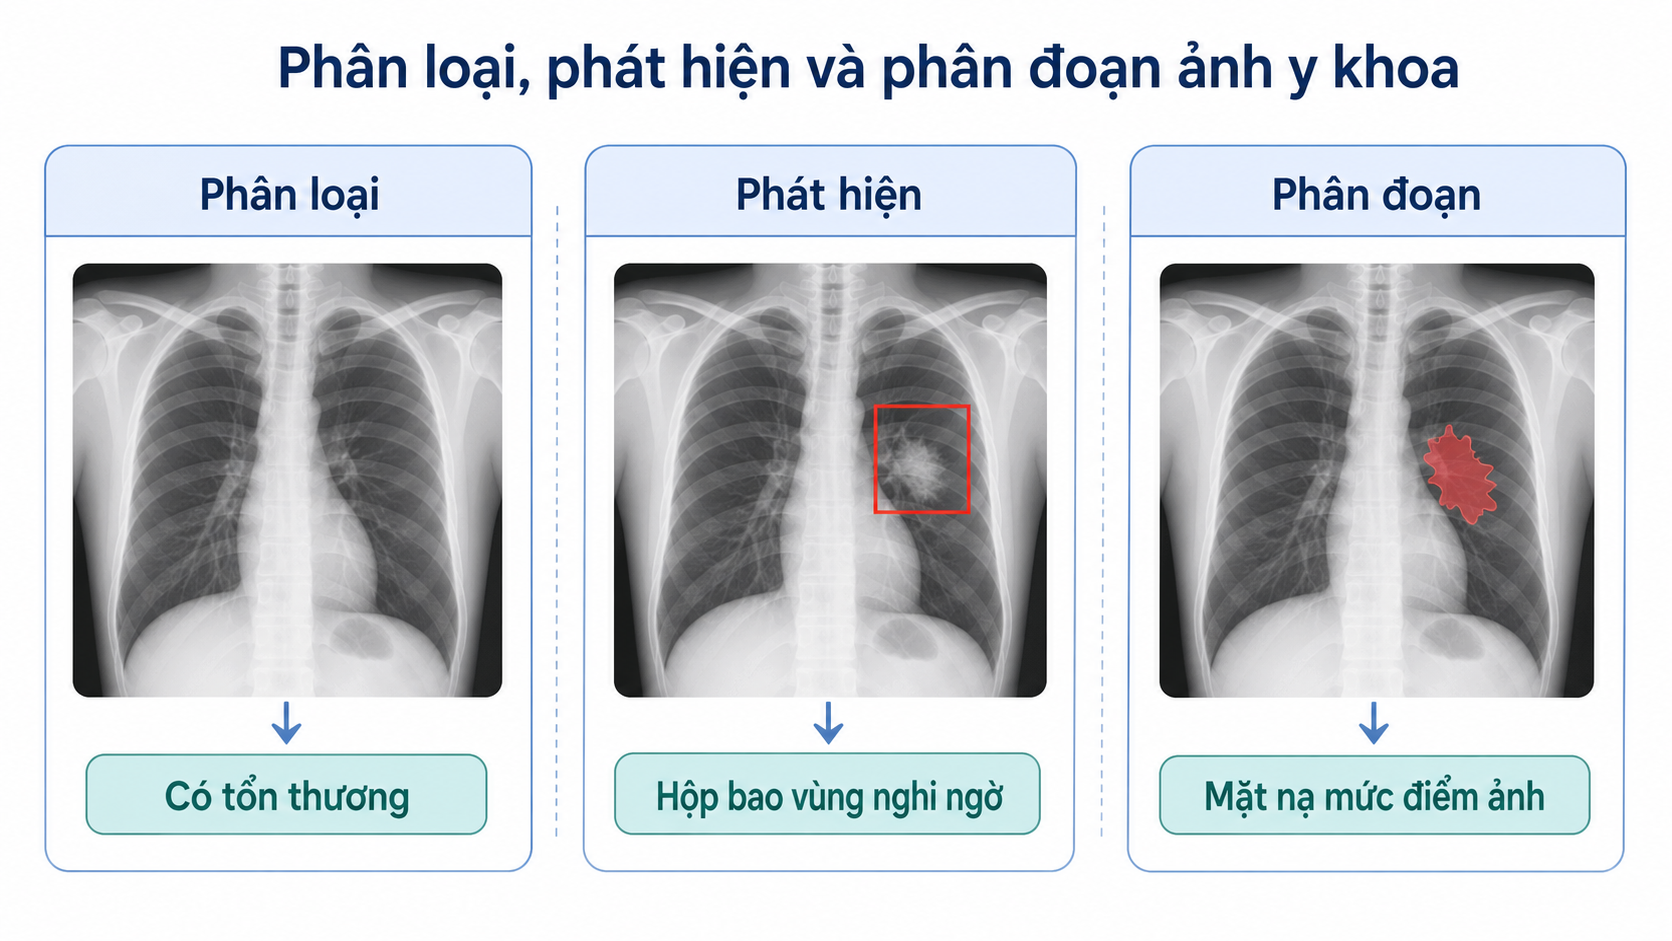
\includegraphics[width=\textwidth]{medical_segmentation_tasks_generated.png}
  \caption{Khác biệt trực quan giữa phân loại, phát hiện và phân đoạn. LViT tập trung vào phân đoạn, tức là dự đoán vùng tổn thương ở mức điểm ảnh thay vì chỉ quyết định ảnh có bệnh hay vẽ một hộp bao thô.}
  \label{fig:classification-detection-segmentation}
\end{figure}

Hình~\ref{fig:classification-detection-segmentation} cho thấy vì sao phân đoạn là một dạng dự đoán dày đặc. Với phân loại, đầu ra có thể chỉ là một nhãn như ``có tổn thương'' hoặc ``không có tổn thương''. Với phát hiện đối tượng, đầu ra thường là một hộp bao hoặc một vùng thô. Với phân đoạn, đầu ra là một bản đồ có cấu trúc không gian: mỗi điểm ảnh được dự đoán thuộc lớp nền hay lớp tổn thương/cơ quan. Độ khó vì thế tăng lên rõ rệt. Một mô hình phân đoạn sai vài điểm ảnh ở biên có thể làm thay đổi diện tích tổn thương; sai một vùng nhỏ nhưng quan trọng có thể ảnh hưởng đến đánh giá mức độ bệnh.

Trong y khoa, đầu ra dạng mặt nạ có nhiều ý nghĩa thực tế. Ở ảnh X-quang hoặc CT phổi, mặt nạ tổn thương giúp ước lượng mức độ lan tỏa của vùng bệnh, hỗ trợ theo dõi diễn tiến và cung cấp tín hiệu định lượng cho bác sĩ. Trong xạ trị, mặt nạ khối u hoặc cơ quan nguy cấp có thể liên quan trực tiếp đến kế hoạch chiếu xạ. Do đó, phân đoạn không chỉ là một bài toán kỹ thuật; nó là bước trung gian để biến ảnh thành thông tin định lượng có thể đo đạc, so sánh và theo dõi.

Tuy nhiên, ảnh y khoa có nhiều đặc điểm làm bài toán phân đoạn khó hơn ảnh tự nhiên. Thứ nhất, biên của cấu trúc bệnh lý thường mờ. Một vùng viêm phổi trên X-quang có thể chuyển tiếp dần sang mô lành, không tạo ranh giới sắc như biên của một chiếc xe hay một người trong ảnh tự nhiên. Thứ hai, độ tương phản giữa tổn thương và nền giải phẫu có thể thấp; tổn thương nhỏ dễ bị che bởi xương sườn, mạch máu, nhiễu chụp hoặc cấu trúc mô xung quanh. Thứ ba, cùng một loại bệnh có thể biểu hiện khác nhau giữa bệnh nhân, thiết bị, lát cắt, tư thế chụp và giai đoạn bệnh. Vì vậy, mô hình không thể chỉ học một mẫu hình cố định rồi áp dụng cho mọi ảnh.

Khó khăn tiếp theo nằm ở dữ liệu huấn luyện. Trong học sâu, mô hình phân đoạn cần nhiều cặp ảnh--mặt nạ để học được ánh xạ từ tín hiệu thị giác sang vùng cần khoanh. Nhưng mặt nạ mức điểm ảnh rất đắt: chuyên gia phải đọc ảnh, xác định vùng nghi ngờ, vẽ biên, kiểm tra lại các ca mơ hồ, và đôi khi cần nhiều người thống nhất nhãn. Công việc này tốn thời gian hơn nhiều so với gán nhãn cấp ảnh. Hệ quả là các bộ dữ liệu y khoa thường rơi vào tình trạng mất cân bằng: ảnh có thể tương đối nhiều, nhưng mặt nạ chất lượng cao lại ít; một số ảnh có mô tả lâm sàng nhưng chưa có vùng khoanh chi tiết.

\begin{figure}[H]
  \centering
  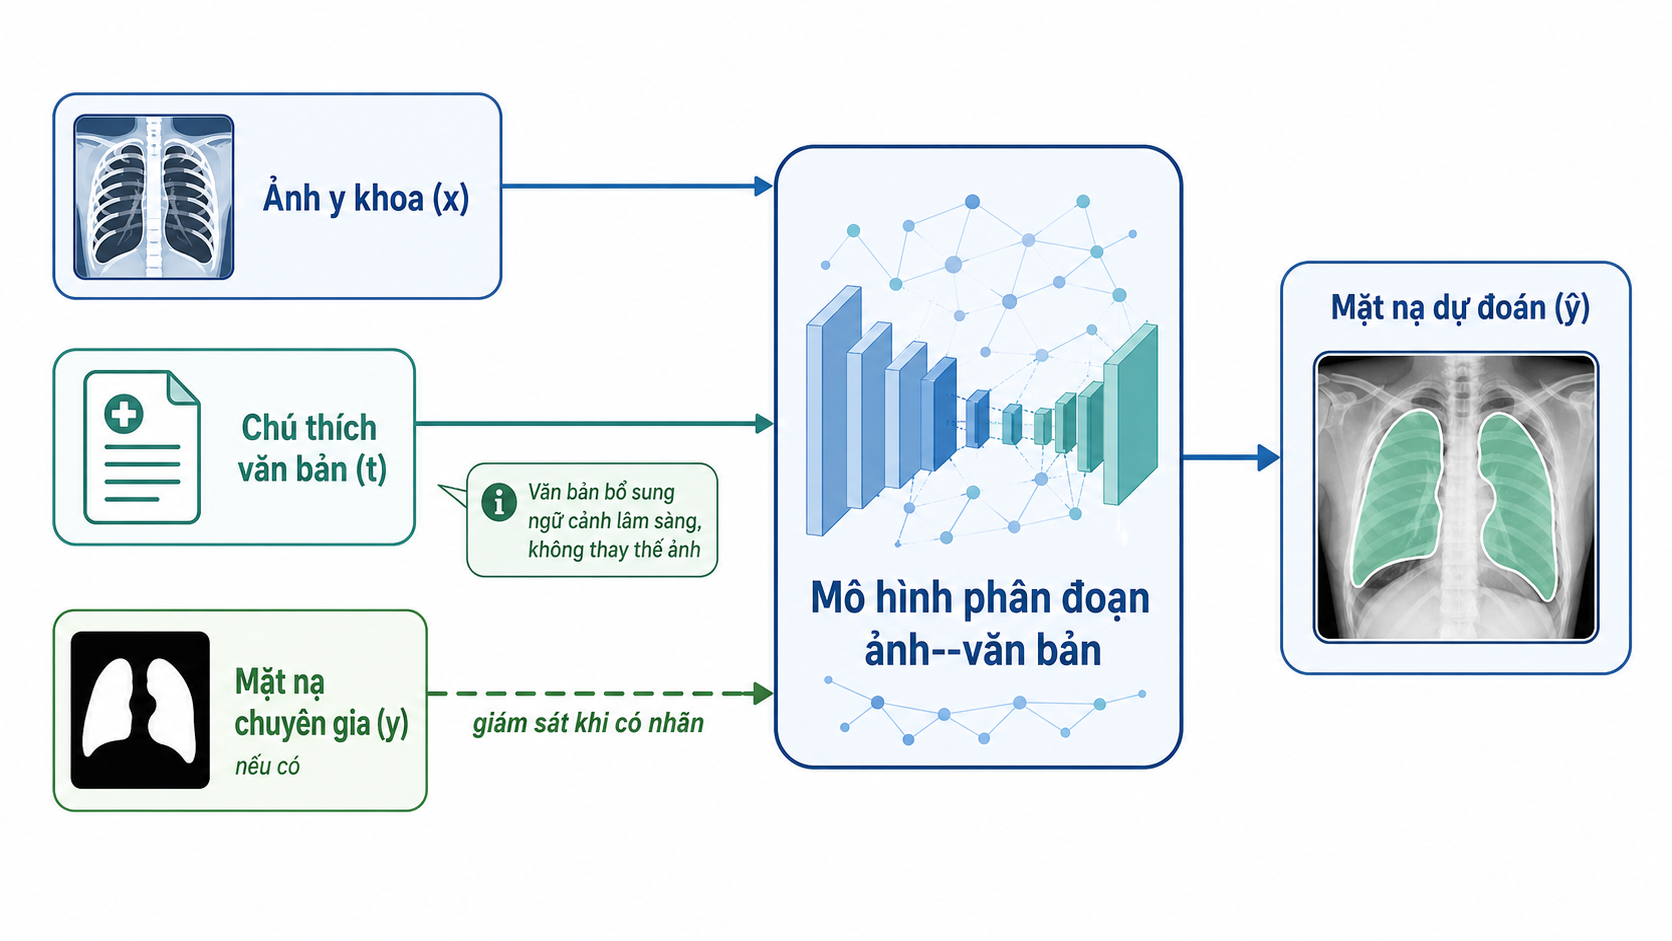
\includegraphics[width=\textwidth]{lvit_data_context_generated.png}
  \caption{Bối cảnh dữ liệu của phân đoạn y khoa có văn bản đi kèm. Ảnh là nguồn tín hiệu thị giác chính, mặt nạ là ground truth đắt đỏ, còn văn bản là nguồn thông tin bổ trợ thường sẵn có hơn mặt nạ chi tiết.}
  \label{fig:lvit-data-context}
\end{figure}

Điểm đáng chú ý trong bối cảnh của LViT là dữ liệu y khoa không chỉ có ảnh. Trong nhiều quy trình lâm sàng, khi bác sĩ đọc ảnh, họ để lại mô tả hoặc ghi chú như vị trí tổn thương, mức độ lan tỏa, vùng giải phẫu liên quan, hoặc nhận xét về tính chất bất thường. Những mô tả này không chi tiết đến mức thay thế được mặt nạ điểm ảnh, nhưng chúng có giá trị ngữ nghĩa. Ví dụ, nếu văn bản nói tổn thương nằm chủ yếu ở vùng dưới phổi trái, mô hình có thêm một gợi ý về không gian và ngữ cảnh; nếu văn bản nói tổn thương lan tỏa hai bên, mô hình có thêm tín hiệu rằng vùng dự đoán không nên chỉ tập trung vào một điểm nhỏ biệt lập.

Bài báo LViT xuất phát chính từ quan sát này. Các tác giả cho rằng hiệu năng của mô hình phân đoạn y khoa bị giới hạn bởi chi phí thu thập dữ liệu có nhãn chất lượng cao, và đề xuất đưa medical văn bản chú thích vào mô hình để bù cho phần thiếu hụt thông tin trong ảnh cũng như cải thiện chất lượng nhãn giả trong học bán giám sát \cite{li2023lvit}. Nói theo ngôn ngữ của Hình~\ref{fig:lvit-data-context}, LViT cố gắng sử dụng cả ba nguồn: ảnh \(x\), văn bản \(t\), và mặt nạ \(y\) khi có. Khi \(y\) không có, văn bản vẫn có thể giúp mô hình tạo hoặc kiểm soát tín hiệu học tạm thời.

Từ đây có thể thấy vì sao LViT không đơn thuần là một biến thể kiến trúc. Nó phản ánh một thay đổi trong cách nhìn bài toán: thay vì xem phân đoạn y khoa là bài toán chỉ dựa trên ảnh, LViT xem mỗi mẫu bệnh án/ảnh như một trường hợp đa nguồn, trong đó ảnh cung cấp hình thái, văn bản cung cấp ngữ nghĩa lâm sàng, và mặt nạ cung cấp giám sát chính xác nhưng đắt đỏ. Chính bối cảnh này dẫn đến lựa chọn phương pháp ở các chương sau: cần một mô hình vừa giữ được chi tiết không gian của ảnh, vừa có cơ chế đưa văn bản vào biểu diễn, vừa có cách học từ dữ liệu chưa nhãn một cách thận trọng.

\section{Động lực nghiên cứu}

Từ bối cảnh ở mục 1.1, động lực nghiên cứu của LViT có thể hiểu như một nỗ lực giải quyết đồng thời ba nút thắt: ảnh y khoa khó diễn giải chỉ bằng tín hiệu thị giác, mặt nạ mức điểm ảnh rất đắt, còn văn bản lâm sàng lại thường tồn tại nhưng chưa được khai thác đúng mức. Triết lý của LViT là không xem ba nguồn thông tin này tách rời nhau. Nếu ảnh cho biết hình thái, văn bản cho biết ngữ nghĩa lâm sàng, và mặt nạ cho biết vùng đúng nhưng khan hiếm, thì một mô hình phân đoạn tốt nên học cách phối hợp các nguồn đó thay vì chỉ tối ưu trên ảnh và mặt nạ.

\begin{figure}[H]
  \centering
  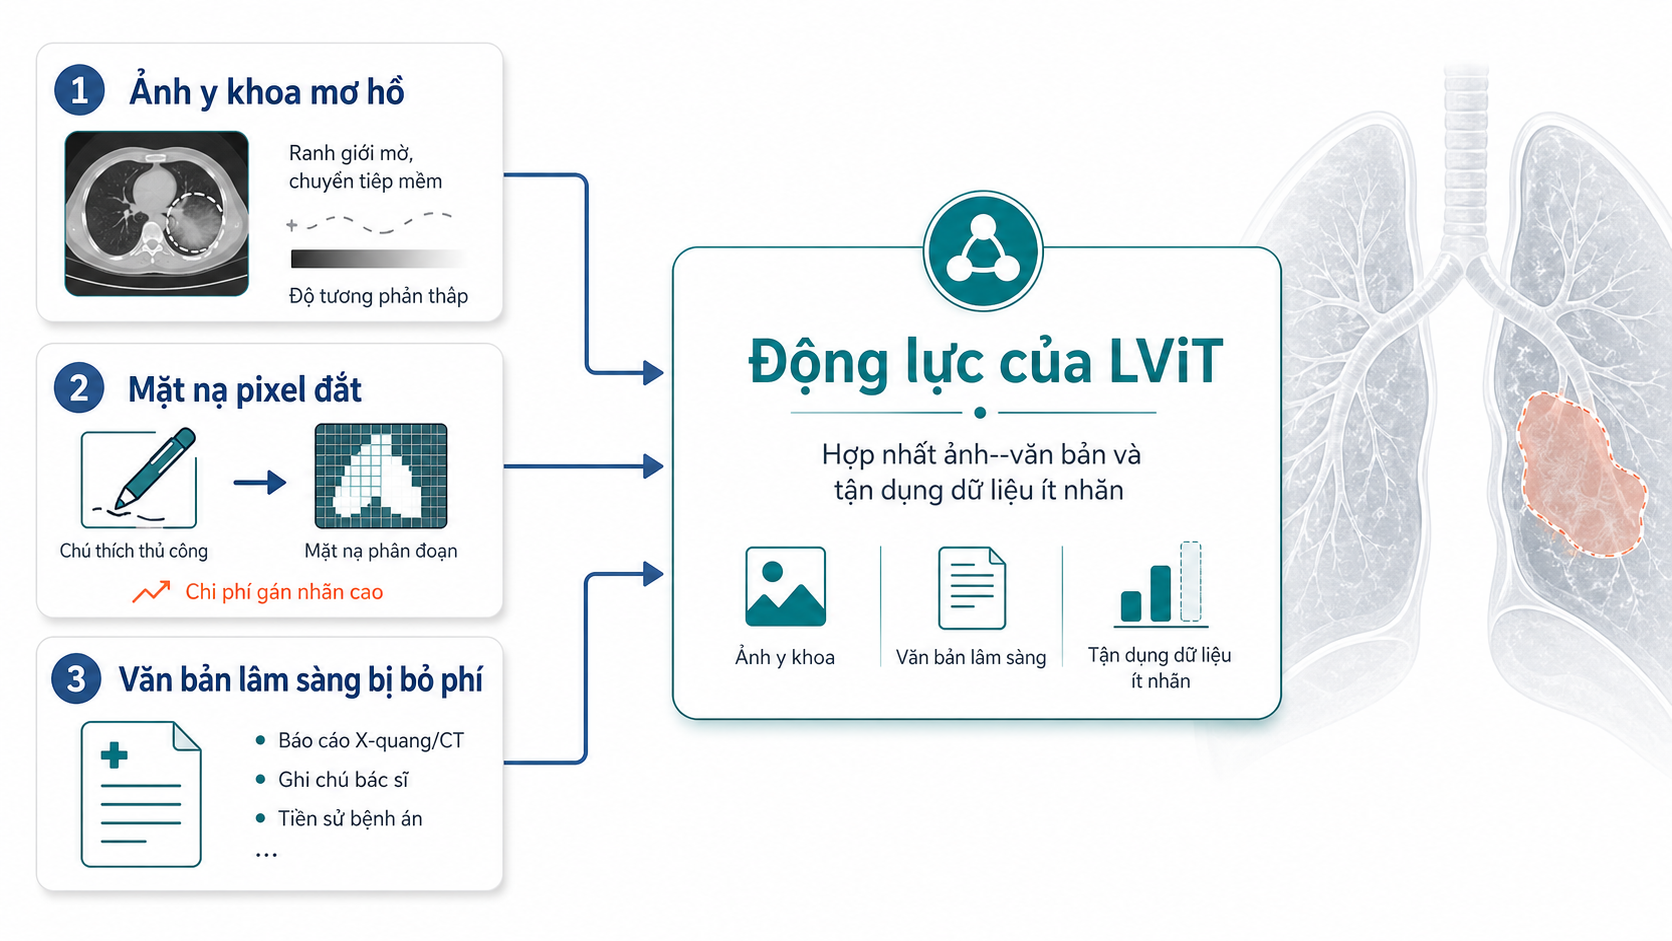
\includegraphics[width=\textwidth]{lvit_motivation_generated.png}
  \caption{Ba động lực chính dẫn đến LViT: độ mơ hồ của ảnh y khoa, chi phí mặt nạ điểm ảnh và nguồn văn bản lâm sàng chưa được khai thác đầy đủ.}
  \label{fig:lvit-motivation}
\end{figure}
\subsection{Ý nghĩa khoa học}

Về mặt khoa học, LViT đặt ra một câu hỏi sâu hơn so với việc chỉ thay backbone phân đoạn: làm thế nào để hợp nhất ảnh và văn bản trong một bài toán dự đoán dày đặc. Ở bài toán phân loại ảnh, mô hình chỉ cần tạo một quyết định cấp ảnh, ví dụ ảnh có bệnh hay không. Khi đó, văn bản có thể được dùng để học một biểu diễn chung cấp ảnh. Nhưng ở phân đoạn, đầu ra là một mặt nạ theo từng điểm ảnh; vì vậy thông tin văn bản phải ảnh hưởng đến không gian ảnh một cách tinh tế hơn. Nếu văn bản nói tổn thương nằm ở vùng dưới phổi trái, mô hình không chỉ cần hiểu câu đó, mà còn phải biến hiểu biết đó thành thay đổi trong đặc trưng không gian và xác suất điểm ảnh.

Đây chính là lý do LViT có ý nghĩa như một bài toán thị giác--ngôn ngữ chuyên biệt cho y khoa. Trước LViT, nhiều phương pháp thị giác--ngôn ngữ đã thành công trong các tác vụ như phân loại, truy hồi ảnh--văn bản hoặc phân đoạn theo mô tả tham chiếu. Tuy nhiên, văn bản y khoa khác văn bản mô tả ảnh tự nhiên. Nó thường ngắn, có tính quy ước, chứa các mô tả giải phẫu hoặc vị trí bệnh, và đôi khi không gọi tên đối tượng theo kiểu trực quan. Vì vậy, không thể chỉ lấy một mô hình thị giác--ngôn ngữ tổng quát rồi gắn vào bài toán y khoa mà không suy nghĩ lại cách văn bản đi vào đặc trưng ảnh.

LViT cũng đặt ra một câu hỏi khoa học thứ hai: khi thiếu mặt nạ thật, văn bản có thể giúp học bán giám sát như thế nào. Trong học bán giám sát, mô hình thường tạo nhãn giả cho dữ liệu chưa nhãn. Nhưng nhãn giả có rủi ro: nếu dự đoán ban đầu sai, mô hình có thể học theo chính sai lầm của nó. Bài báo LViT đề xuất Exponential Pseudo-label Iteration (EPI) để làm mượt nhãn giả qua thời gian và Language--Vision loss để dùng thông tin văn bản giám sát trực tiếp dữ liệu chưa nhãn \cite{li2023lvit}. Ý nghĩa ở đây không chỉ là thêm một loss mới, mà là đưa văn bản vào vai trò kiểm soát chất lượng học khi mặt nạ thật vắng mặt.

Nhìn theo ba hướng lớn của phân đoạn y khoa, động lực khoa học của LViT nằm ở vùng giao giữa dựa vào bản đồ đặc trưng CNN, token-based Transformer và vision-language learning. CNN có thiên kiến cục bộ tốt cho biên và cấu trúc nhỏ. Transformer có khả năng mô hình hóa quan hệ xa. Văn bản cung cấp ngữ nghĩa mà ảnh có thể không biểu hiện rõ. LViT có ý nghĩa vì nó thử kết nối ba nguồn năng lực này vào một hệ thống phân đoạn thống nhất thay vì xem chúng như các dòng nghiên cứu độc lập.

\subsection{Ý nghĩa thực tiễn}

Về mặt thực tiễn, động lực lớn nhất của LViT là giảm phụ thuộc vào mặt nạ được gán nhãn đầy đủ. Trong bệnh viện hoặc dự án dữ liệu y khoa, việc thu thập ảnh thường dễ hơn việc thu thập mặt nạ chuẩn. Ảnh có thể đã có trong hệ thống lưu trữ, báo cáo hoặc ghi chú có thể đã được tạo trong quy trình đọc ảnh, nhưng mặt nạ chi tiết lại cần thêm nhiều giờ lao động chuyên gia. Nếu một phương pháp chỉ hoạt động tốt khi có nhiều mặt nạ hoàn chỉnh, nó sẽ khó triển khai trong các bối cảnh dữ liệu nhỏ, bệnh mới hoặc cơ sở y tế chưa có đội ngũ gán nhãn lớn.

\begin{figure}[H]
  \centering
  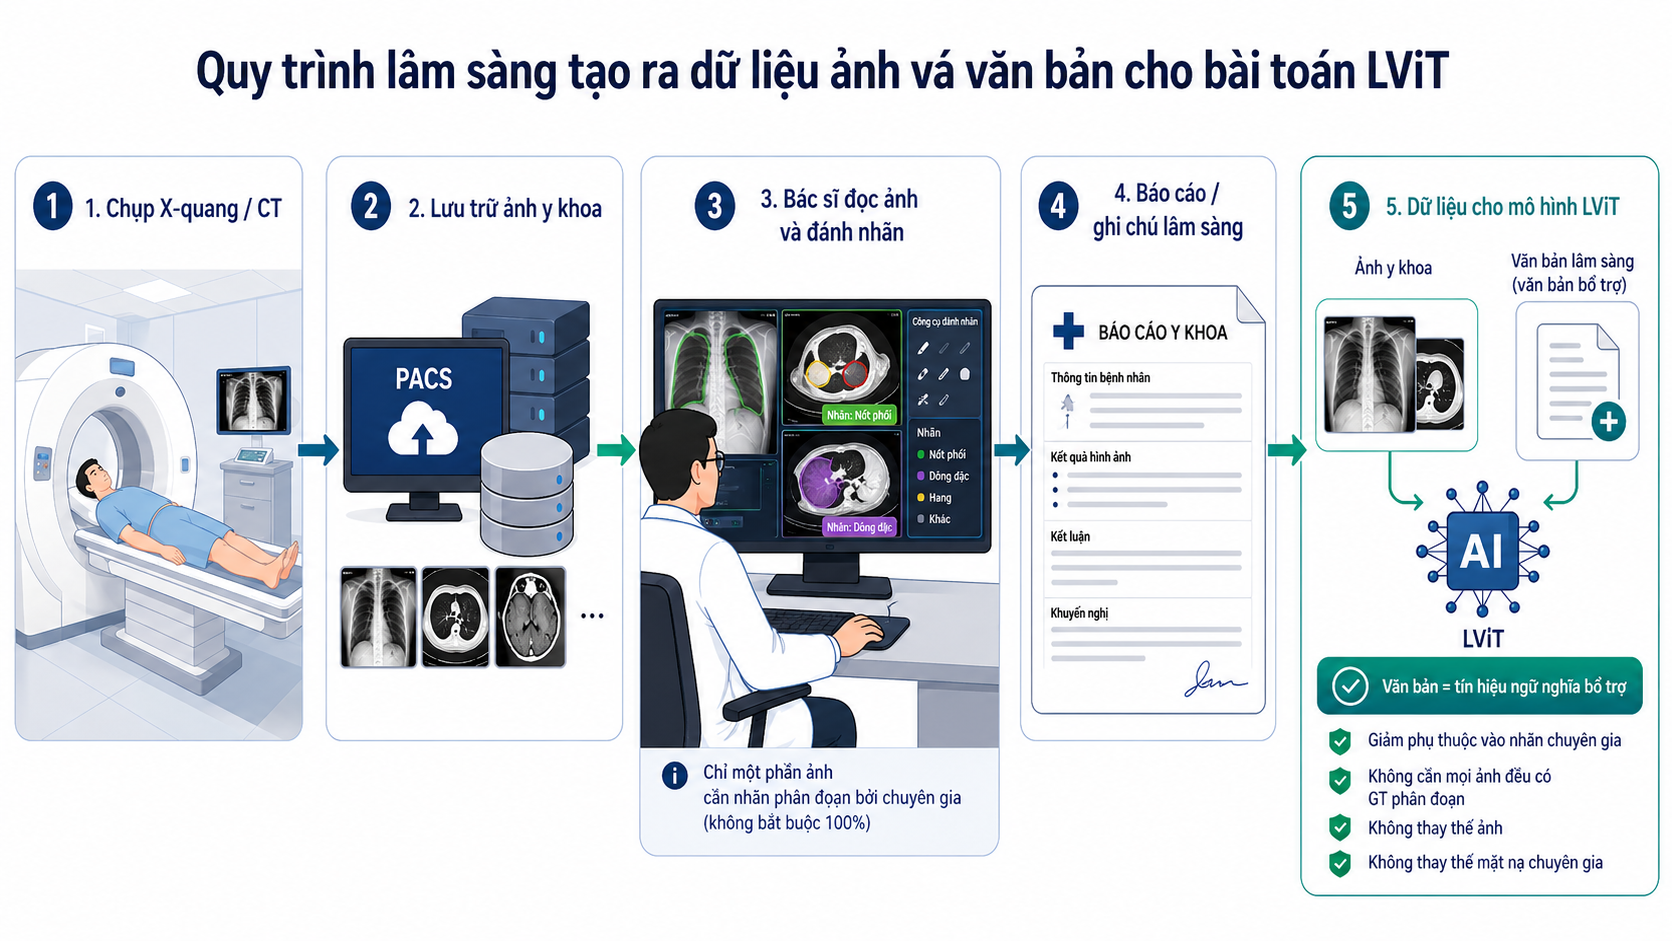
\includegraphics[width=\textwidth]{clinical_text_workflow_generated.png}
  \caption{Quy trình lâm sàng tạo ra dữ liệu ảnh và văn bản cho LViT. Ảnh y khoa được lưu trữ sau khi chụp, bác sĩ đọc ảnh và tạo báo cáo/ghi chú; phần văn bản này trở thành tín hiệu ngữ nghĩa bổ trợ cho mô hình, nhưng không thay thế ảnh đầu vào hoặc mặt nạ chuyên gia.}
  \label{fig:clinical-văn bản-workflow}
\end{figure}

LViT giải quyết vấn đề này theo một hướng thực tế: tận dụng văn bản chú thích như một loại thông tin trung gian rẻ hơn mặt nạ. Văn bản không thay thế bác sĩ và cũng không thay thế mặt nạ ground truth, nhưng nó có thể cung cấp gợi ý về vị trí, mức độ và loại bất thường. Khi được đưa vào mô hình đúng cách, văn bản có thể giúp mô hình bớt phụ thuộc vào tín hiệu ảnh thuần túy, đặc biệt trong các ca biên mờ hoặc tổn thương khó phân biệt với nền giải phẫu.

Ý nghĩa thực tiễn thứ hai là khả năng tận dụng dữ liệu chưa nhãn. Nhiều tập dữ liệu có thể chứa ảnh và báo cáo nhưng thiếu mặt nạ. Nếu mô hình có thể tạo nhãn giả ổn định hơn nhờ EPI và được văn bản hỗ trợ bằng LV loss, thì các mẫu chưa có mặt nạ vẫn có thể đóng góp vào quá trình học \cite{li2023lvit}. Điều này mở ra một hướng triển khai hợp lý hơn cho y khoa: thay vì đợi đến khi mọi ảnh đều được khoanh vùng thủ công, có thể bắt đầu từ một phần nhỏ dữ liệu có mặt nạ và một phần lớn dữ liệu có ảnh--văn bản.

Ý nghĩa thực tiễn thứ ba là làm cho hệ thống phân đoạn gần hơn với cách dữ liệu y khoa thật được sinh ra. Trong thực tế, một ca ảnh y khoa không tồn tại như một ma trận điểm ảnh trơ trọi; nó đi kèm bối cảnh bệnh nhân, mô tả của bác sĩ, chỉ định chụp, vùng nghi ngờ và nhiều thông tin bán cấu trúc khác. LViT chưa giải quyết toàn bộ bài toán hồ sơ bệnh án, nhưng nó là một bước quan trọng: đưa ít nhất một phần ngôn ngữ y khoa vào mô hình phân đoạn. Đây là lý do báo cáo chọn LViT làm phương pháp trung tâm để khảo sát.

Tóm lại, động lực nghiên cứu của LViT không chỉ là đạt thêm vài điểm Dice hoặc IoU. Động lực sâu hơn là thay đổi cách xây dựng hệ thống phân đoạn y khoa trong điều kiện dữ liệu thực tế: ít mặt nạ, ảnh khó, nhưng có văn bản giàu ngữ nghĩa. Chính động lực này sẽ dẫn sang mục 1.3, nơi bài toán được phát biểu chính thức bằng đầu vào, đầu ra, ground truth và các công đoạn chung của hệ thống.

\section{Phát biểu bài toán}

Phát biểu bài toán là bước chuyển từ động lực nghiên cứu sang một mô hình hóa rõ ràng: hệ thống nhận những dữ liệu nào, phải sinh ra kết quả gì, và trong quá trình học cần tìm những đại lượng ẩn nào. Triết lý ở đây là không mô tả ngay một kiến trúc cụ thể như một đáp án duy nhất, mà trước hết phải nhìn bài toán như một chuỗi công đoạn chung. Khi chuỗi công đoạn đã rõ, ta mới thấy LViT đóng góp vào đâu: mã hóa ảnh và văn bản, hợp nhất hai nguồn thông tin, kết hợp CNN--Transformer, kiểm soát pseudo-label trong bán giám sát và cuối cùng sinh mặt nạ phân đoạn.

\subsection{Dữ liệu đầu vào}

Dữ liệu đầu vào cần được hiểu như một ca ảnh y khoa có ngữ cảnh, không chỉ là một ma trận điểm ảnh. Với mỗi mẫu, hệ thống nhận ảnh y khoa \(x\) và mô tả văn bản đi kèm \(t\). Trong phạm vi báo cáo, ảnh \(x\) chủ yếu là X-quang ngực hoặc lát cắt CT phổi đã được đưa về kích thước chuẩn. Văn bản \(t\) là chú thích hoặc báo cáo lâm sàng ngắn, thường chứa các thông tin như bên tổn thương, số vùng bất thường, mức độ lan tỏa và vị trí giải phẫu xấp xỉ.

Trong ký hiệu của bài toán, dữ liệu có nhãn được viết là:
\[
\mathcal{D}_l=\{(x_i,t_i,y_i)\}_{i=1}^{N_l},
\]
trong đó \(y_i\) là mặt nạ phân đoạn do chuyên gia hoặc bộ dữ liệu chuẩn cung cấp. Dữ liệu chưa nhãn được viết là:
\[
\mathcal{D}_u=\{(x_j,t_j)\}_{j=1}^{N_u},
\]
tức là vẫn có ảnh và văn bản, nhưng chưa có mặt nạ \(y\). Cách viết này quan trọng vì LViT không chỉ khai thác ảnh--mặt nạ trong học có giám sát, mà còn dùng ảnh--văn bản ở phần chưa nhãn để cải thiện học bán giám sát.

\subsection{Đầu ra của hệ thống}

Đầu ra của hệ thống là mặt nạ dự đoán \(\hat{y}\) có cùng không gian với ảnh đầu vào:
\[
\hat{y}=f(x,t).
\]
Nếu bài toán là nhị phân, \(\hat{y}_{u,v}\in[0,1]\) biểu diễn xác suất điểm ảnh \((u,v)\) thuộc vùng tổn thương/cơ quan cần tách. Nếu bài toán có nhiều lớp, đầu ra có thể là một vector xác suất cho từng lớp tại mỗi điểm ảnh. Sau khi có bản đồ xác suất, hệ thống có thể áp dụng ngưỡng để tạo mặt nạ nhị phân dùng cho đánh giá hoặc hiển thị.

Khác với phân loại ảnh, đầu ra ở đây không phải một nhãn duy nhất như ``có bệnh'' hay ``không có bệnh''. Mặt nạ \(\hat{y}\) phải giữ cấu trúc không gian: vùng nào thuộc tổn thương, vùng nào là nền, biên nằm ở đâu và diện tích vùng bệnh lớn bao nhiêu. Vì vậy, độ chính xác của hệ thống không chỉ được nhìn bằng một tỉ lệ đúng/sai tổng quát, mà thường dùng Dice và IoU/mIoU để đo mức chồng lấp giữa mặt nạ dự đoán và mặt nạ chuẩn.

\subsection{Nhãn xác thực và vai trò của mặt nạ}

Nhãn xác thực, hay ground truth, là mặt nạ \(y\) được gán ở mức điểm ảnh. Với mỗi điểm ảnh, \(y_{u,v}=1\) nếu điểm đó thuộc vùng cần phân đoạn và \(y_{u,v}=0\) nếu thuộc nền trong bài toán nhị phân. Trong giai đoạn học có giám sát, mô hình tối ưu các tham số để \(\hat{y}\) gần \(y\). Các loss thường dùng như Dice loss, cross-entropy hoặc BCE đều có liên hệ trực tiếp với mục tiêu này: BCE/cross-entropy ép xác suất từng điểm ảnh đúng lớp, còn Dice loss ép vùng dự đoán chồng lấp tốt với vùng thật.

Điểm cần nhấn mạnh là \(y\) rất đắt. Nó không phải nhãn có thể lấy tự động từ báo cáo, mà thường cần chuyên gia vẽ biên và kiểm tra. Trong giai đoạn bán giám sát, khi một mẫu chỉ có \((x,t)\), hệ thống không thể tính loss trực tiếp với \(y\). Khi đó, mô hình phải tạo mục tiêu tạm thời như pseudo-label \(\tilde{y}\), hoặc dùng ràng buộc từ văn bản để kiểm soát dự đoán. Đây là lý do bài toán của LViT không chỉ là ``ảnh cộng văn bản ra mặt nạ'', mà còn là bài toán học trong điều kiện mặt nạ thật không luôn sẵn có.

\subsection{Các bộ dữ liệu LViT quan tâm}

Các bộ dữ liệu là nơi làm rõ đầu vào, đầu ra và nhãn xác thực ở trên. Báo cáo này tập trung vào hai bộ dữ liệu đa phương thức ảnh--văn bản gắn trực tiếp với bài toán COVID-19 trong LViT: QaTa-COV19 và MosMedData+ \cite{li2023lvit,lvitOfficialRepo}. Hai tập này giúp nhìn bài toán ở hai miền ảnh phổi khác nhau: X-quang ngực và CT phổi. Điểm chung cần chú ý là mỗi mẫu nên được hiểu theo bộ ba \((x,t,y)\): ảnh \(x\), mô tả văn bản \(t\), và mặt nạ \(y\) nếu có. Riêng \(t\) trong các gói dữ liệu LViT không nên hiểu là toàn bộ bệnh án thô; nó là \textit{văn bản chú thích} dạng câu ngắn, có cấu trúc, được nhóm LViT phát hành kèm dữ liệu để mô hình có tín hiệu ngữ nghĩa ổn định.

\begin{table}[H]
  \centering
  \caption{Quy mô và vai trò của hai bộ dữ liệu được dùng để phân tích trong báo cáo.}
  \label{tab:lvit-dataset-splits}
  \small
  \renewcommand{\arraystretch}{1.12}
  \setlength{\tabcolsep}{5pt}
  \begin{tabularx}{\textwidth}{@{}l Y Y Y Y@{}}
    \toprule
    Bộ dữ liệu & Train & Validation & Test & Ghi chú \\
    \midrule
    QaTa-COV19 & 5716 & 1429 & 2113 & 9258 ảnh X-quang COVID-19 trong paper LViT \\
    MosMedData+ & 2183 & 273 & 273 & 2729 lát CT COVID-19 trong paper LViT \\
    \bottomrule
  \end{tabularx}
\end{table}
\FloatBarrier

\textbf{QaTa-COV19} là bộ dữ liệu X-quang ngực COVID-19 gồm 9258 ảnh có manual chú thích vùng tổn thương \cite{degerli2022qatacov19}. Đây là bộ dữ liệu rất phù hợp để kiểm tra ý tưởng của LViT vì X-quang ngực có vị trí giải phẫu tương đối cố định, nhưng tổn thương COVID-19 có biên mờ, độ tương phản thấp và mức lan tỏa khác nhau. văn bản chú thích trong LViT mô tả ba nhóm thông tin chính. Nhóm thứ nhất là \textit{kiểu lan tổn thương}: unilateral hoặc bilateral pulmonary infection. Nhóm thứ hai là \textit{số vùng nhiễm}: one, two, three, ... infected areas. Nhóm thứ ba là \textit{vị trí giải phẫu tương đối}: phổi trái/phải và vùng upper, middle, lower hoặc all lung. Ví dụ câu ``Bilateral pulmonary infection, two infected areas, all left lung and middle lower right lung'' có thể tách thành: nhiễm hai bên, hai vùng nhiễm, toàn bộ phổi trái và vùng giữa--dưới phổi phải. Vì vậy, \(t\) ở đây không thay thế \(y\), nhưng nó cho mô hình một bản mô tả có cấu trúc về nơi nên chú ý.

\begin{figure}[H]
  \centering
  \IfFileExists{figures/dataset_examples_qatacov19.png}{%
    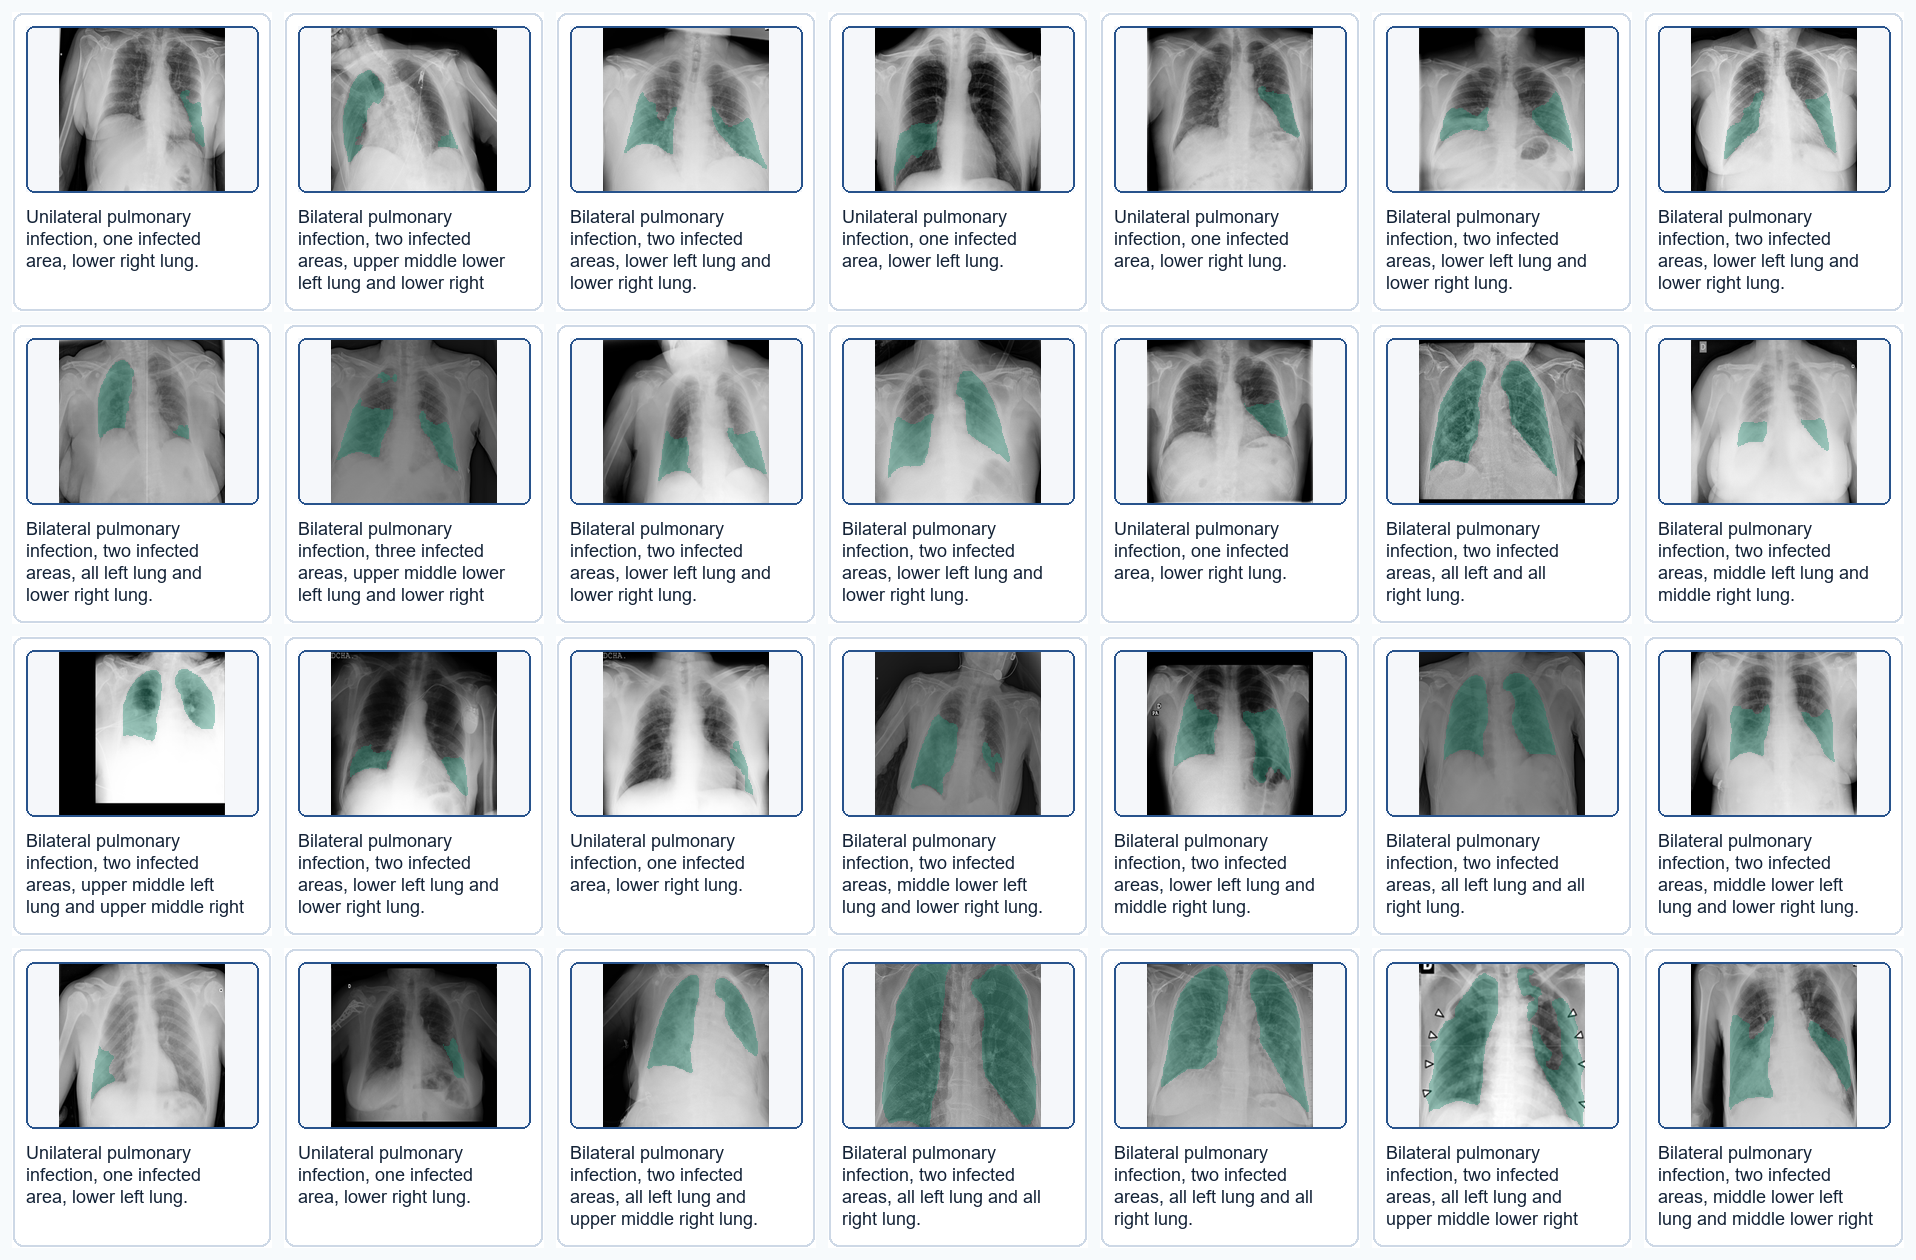
\includegraphics[width=\textwidth]{figures/dataset_examples_qatacov19.png}%
  }{%
    \fbox{\parbox[c][4.2cm][c]{0.92\textwidth}{\centering Hình minh họa 4x7 cặp ảnh--văn bản của QaTa-COV19.}}%
  }
  \caption{Các cặp ảnh--văn bản mẫu của QaTa-COV19. Hình nên thể hiện khoảng 4x7 mẫu để thấy sự đa dạng về vị trí, số vùng và mức độ tổn thương.}
  \label{fig:dataset-examples-qatacov19}
\end{figure}

Phân tích EDA trên toàn bộ 9258 văn bản annotations của QaTa-COV19 cho thấy cấu trúc này xuất hiện rất đều. Có 7338 mẫu bilateral và 1920 mẫu unilateral; phần lớn câu mô tả hai vùng nhiễm, với 6862 mẫu thuộc nhóm này. Ở trường vị trí, các từ khóa left/right lung và upper/middle/lower/all lung xuất hiện lặp lại theo một ngữ pháp gần như cố định. Đây chính là lý do LViT có thể dùng embedding văn bản và LV loss: nếu câu mô tả có cấu trúc ổn định, độ tương đồng giữa văn bản annotations sẽ phản ánh tương đối tốt sự gần nhau về vùng tổn thương.

\begin{figure}[H]
  \centering
  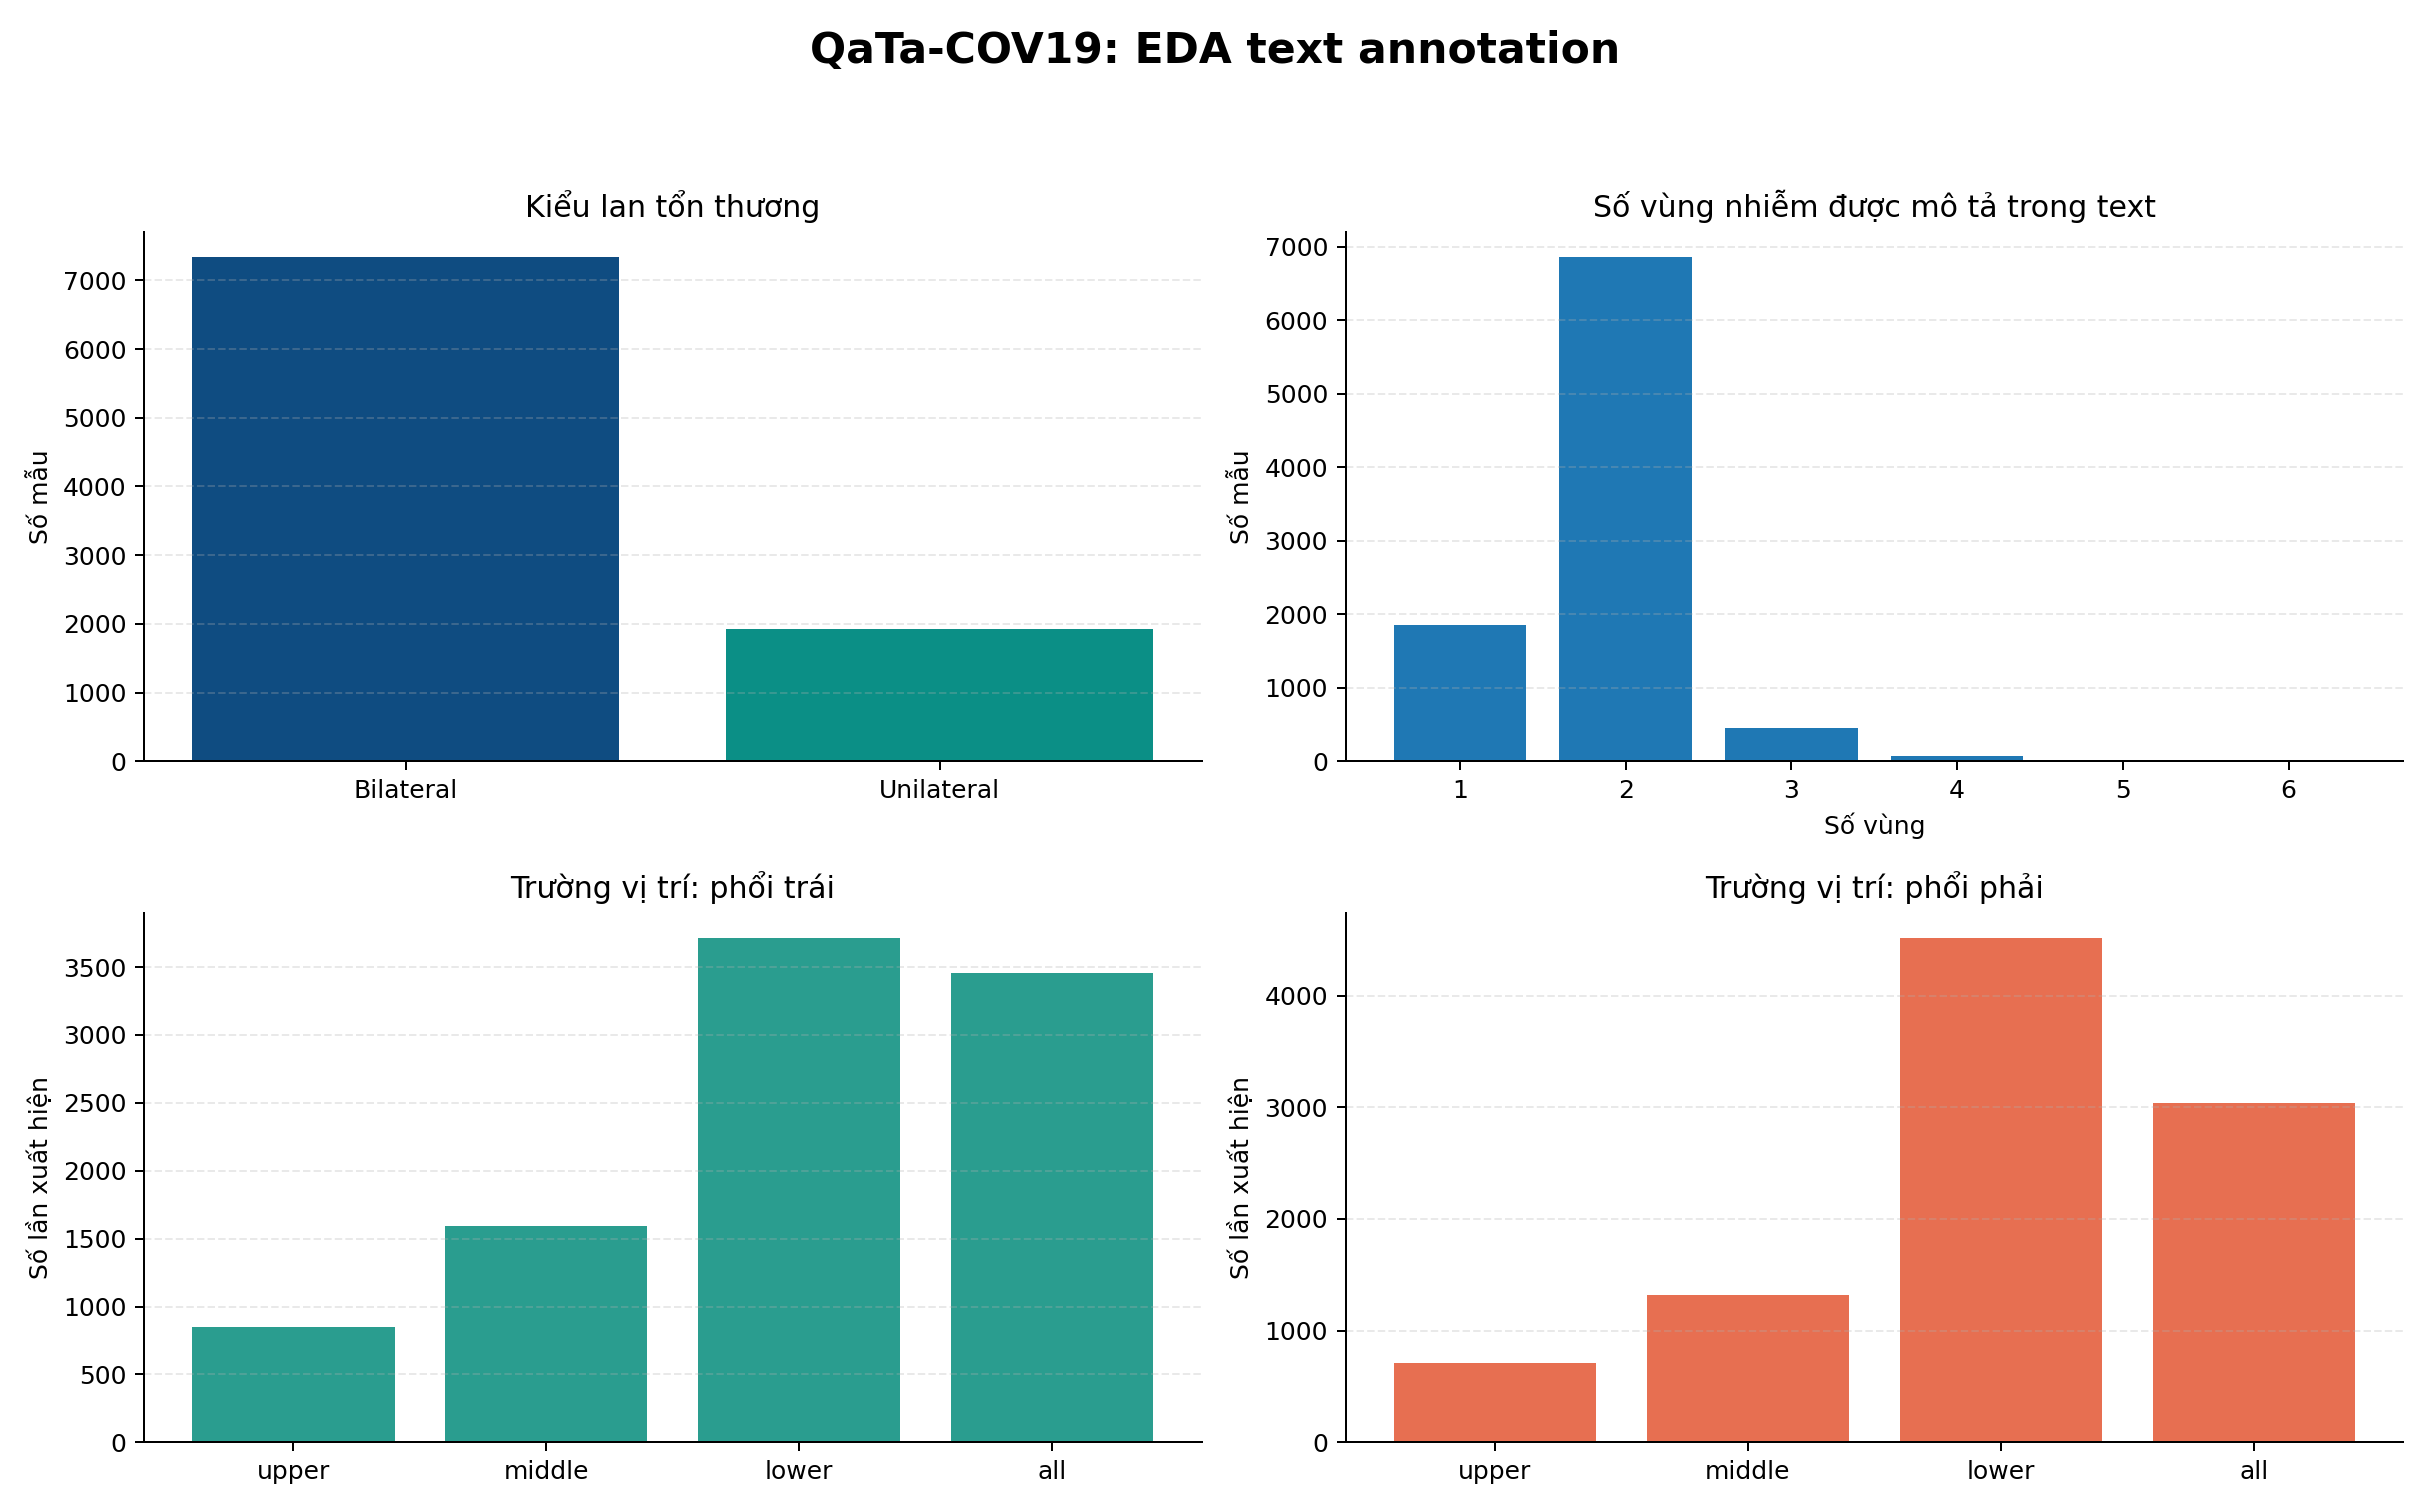
\includegraphics[width=\textwidth]{figures/dataset_text_eda_qatacov19.png}
  \caption{EDA văn bản chú thích của QaTa-COV19. Các biểu đồ cho thấy văn bản có cấu trúc rõ theo kiểu lan tổn thương, số vùng nhiễm và vị trí trái/phải theo vùng phổi.}
  \label{fig:dataset-văn bản-eda-qatacov19}
\end{figure}

\textbf{MosMedData+} là bộ dữ liệu CT phổi COVID-19, trong paper LViT gồm 2729 lát CT có vùng nhiễm trùng phổi \cite{morozov2020mosmeddata,li2023lvit}. Dấu ``+'' ở đây quan trọng: gói MosMedData+ dùng trong LViT không chỉ là MosMedData gốc, mà là một tập CT segmentation được tổng hợp từ nhiều nguồn công khai. Theo cách định danh dữ liệu của nhóm LViT, tập này gồm ba nhóm nguồn chính: nhóm Morozov/MosMedData, nhóm Jun/Coronacases--Radiopaedia, và nhóm Bjørke/MedSeg CT \cite{morozov2020mosmeddata,medicalsegmentationCovid19,lvitOfficialRepo}. Việc gộp nguồn làm dữ liệu đa dạng hơn về bệnh nhân, lát cắt và cách thu nhận ảnh; đổi lại, phân bố tổn thương và chất lượng ảnh cũng không đồng nhất như một bộ dữ liệu đơn nguồn.

\begin{figure}[H]
  \centering
  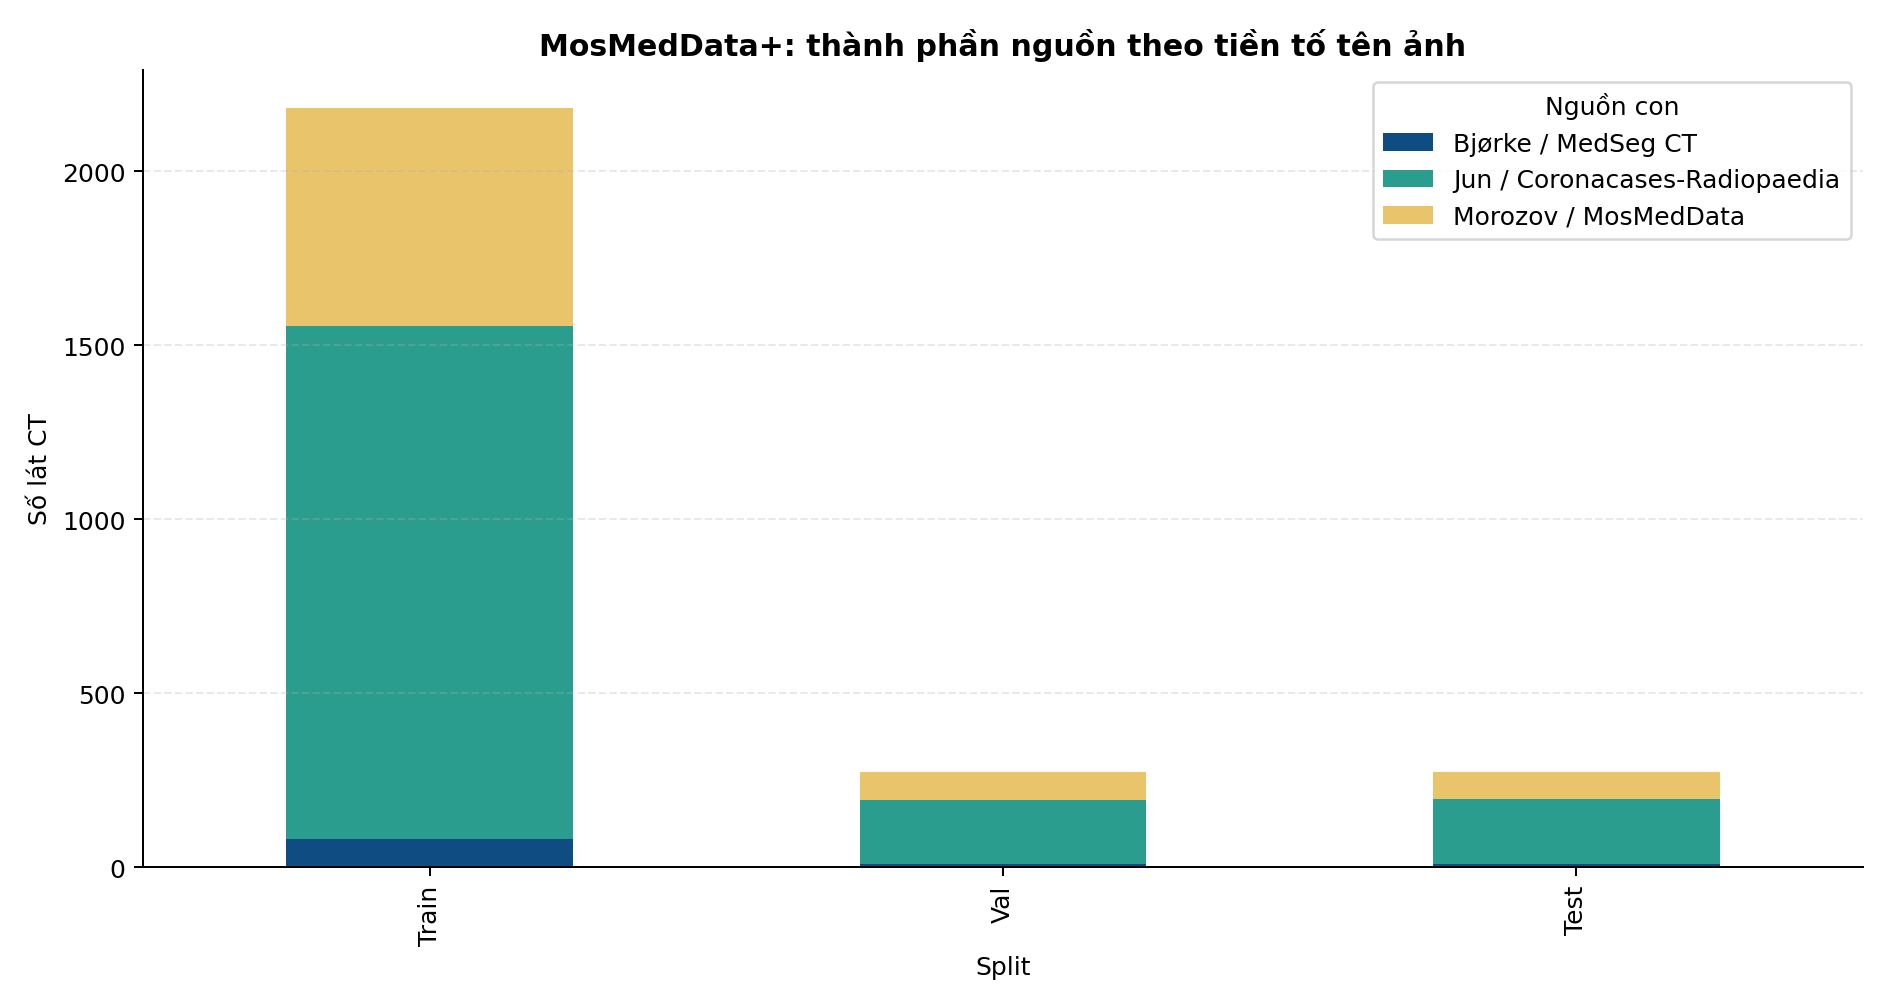
\includegraphics[width=0.92\textwidth]{figures/dataset_sources_mosmeddata.png}
  \caption{Thành phần nguồn của MosMedData+. Nhóm Jun bao gồm các ảnh có nguồn Coronacases/Radiopaedia, nhóm Morozov tương ứng MosMedData, và nhóm Bjørke tương ứng tập CT segmentation trên Medical Segmentation.}
  \label{fig:dataset-sources-mosmeddata}
\end{figure}

So với X-quang, CT chứa thông tin lát cắt chi tiết hơn nhưng cũng tạo ra thách thức khác: tổn thương có thể nhỏ, phân bố rải rác, cường độ thay đổi theo lát cắt và dễ bị ảnh hưởng bởi tiền xử lý vùng phổi. văn bản chú thích của MosMedData+ không phải văn bản lâm sàng nguyên thủy đi kèm từng bệnh nhân, mà là chú thích dạng cấu trúc được phát hành cùng LViT. Nó dùng cùng ngữ pháp với QaTa-COV19: kiểu lan tổn thương, số vùng nhiễm, và vị trí tương đối trên phổi trái/phải. Ví dụ ``Unilateral pulmonary infection, two infected areas, middle lower left lung'' cho biết tổn thương một bên, có hai vùng, nằm ở vùng giữa--dưới phổi trái. Bộ dữ liệu này quan trọng vì nó kiểm tra xem LViT có còn hữu ích khi chuyển từ X-quang 2D sang CT slice hay không.

\begin{figure}[H]
  \centering
  \IfFileExists{figures/dataset_examples_mosmeddata.png}{%
    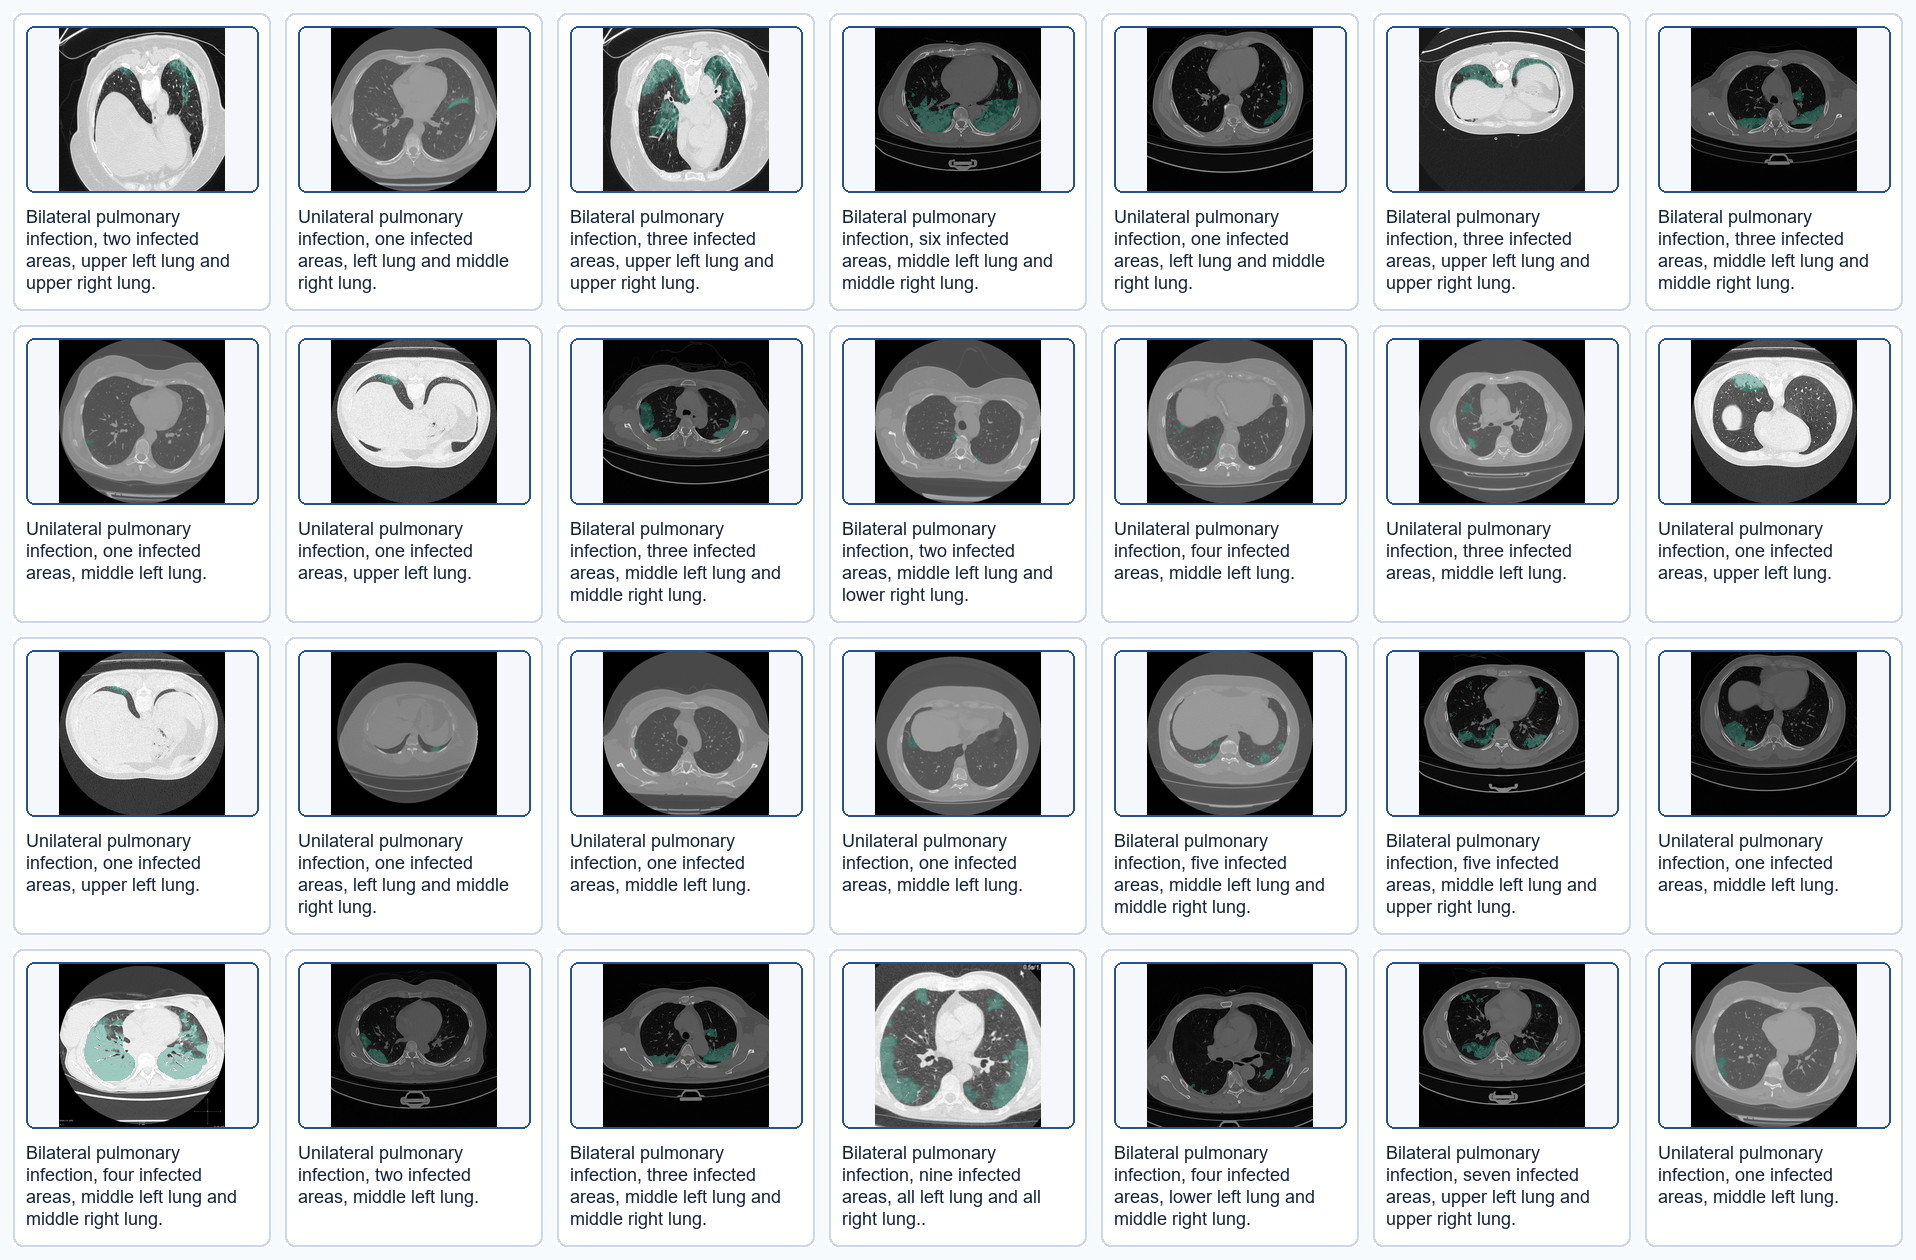
\includegraphics[width=\textwidth]{figures/dataset_examples_mosmeddata.png}%
  }{%
    \fbox{\parbox[c][4.2cm][c]{0.92\textwidth}{\centering Hình minh họa 4x7 cặp ảnh--văn bản của MosMedData+.}}%
  }
  \caption{Các cặp ảnh--văn bản mẫu của MosMedData+. Hình nên cho thấy các lát CT với vùng tổn thương khác nhau và mô tả văn bản tương ứng.}
  \label{fig:dataset-examples-mosmeddata}
\end{figure}

EDA trên 2729 mô tả của MosMedData+ cho thấy văn bản vẫn có cấu trúc, nhưng phân bố khác QaTa-COV19. Số mẫu bilateral và unilateral gần cân bằng: 1342 bilateral, 1340 unilateral, còn 47 mô tả không rơi vào mẫu parse chuẩn. Trường số vùng nhiễm trải rộng hơn, từ một đến chín vùng, cho thấy CT có thể biểu diễn tổn thương rải rác hơn X-quang. Ở trường vị trí, ``middle left lung'' và ``middle right lung'' xuất hiện nhiều, trong khi các mô tả ``all lung'' ít hơn. Điều này làm rõ ý nghĩa của văn bản chú thích: nó không chỉ nói có bệnh hay không, mà mã hóa vị trí tương đối và mức phân mảnh của tổn thương.

\begin{figure}[H]
  \centering
  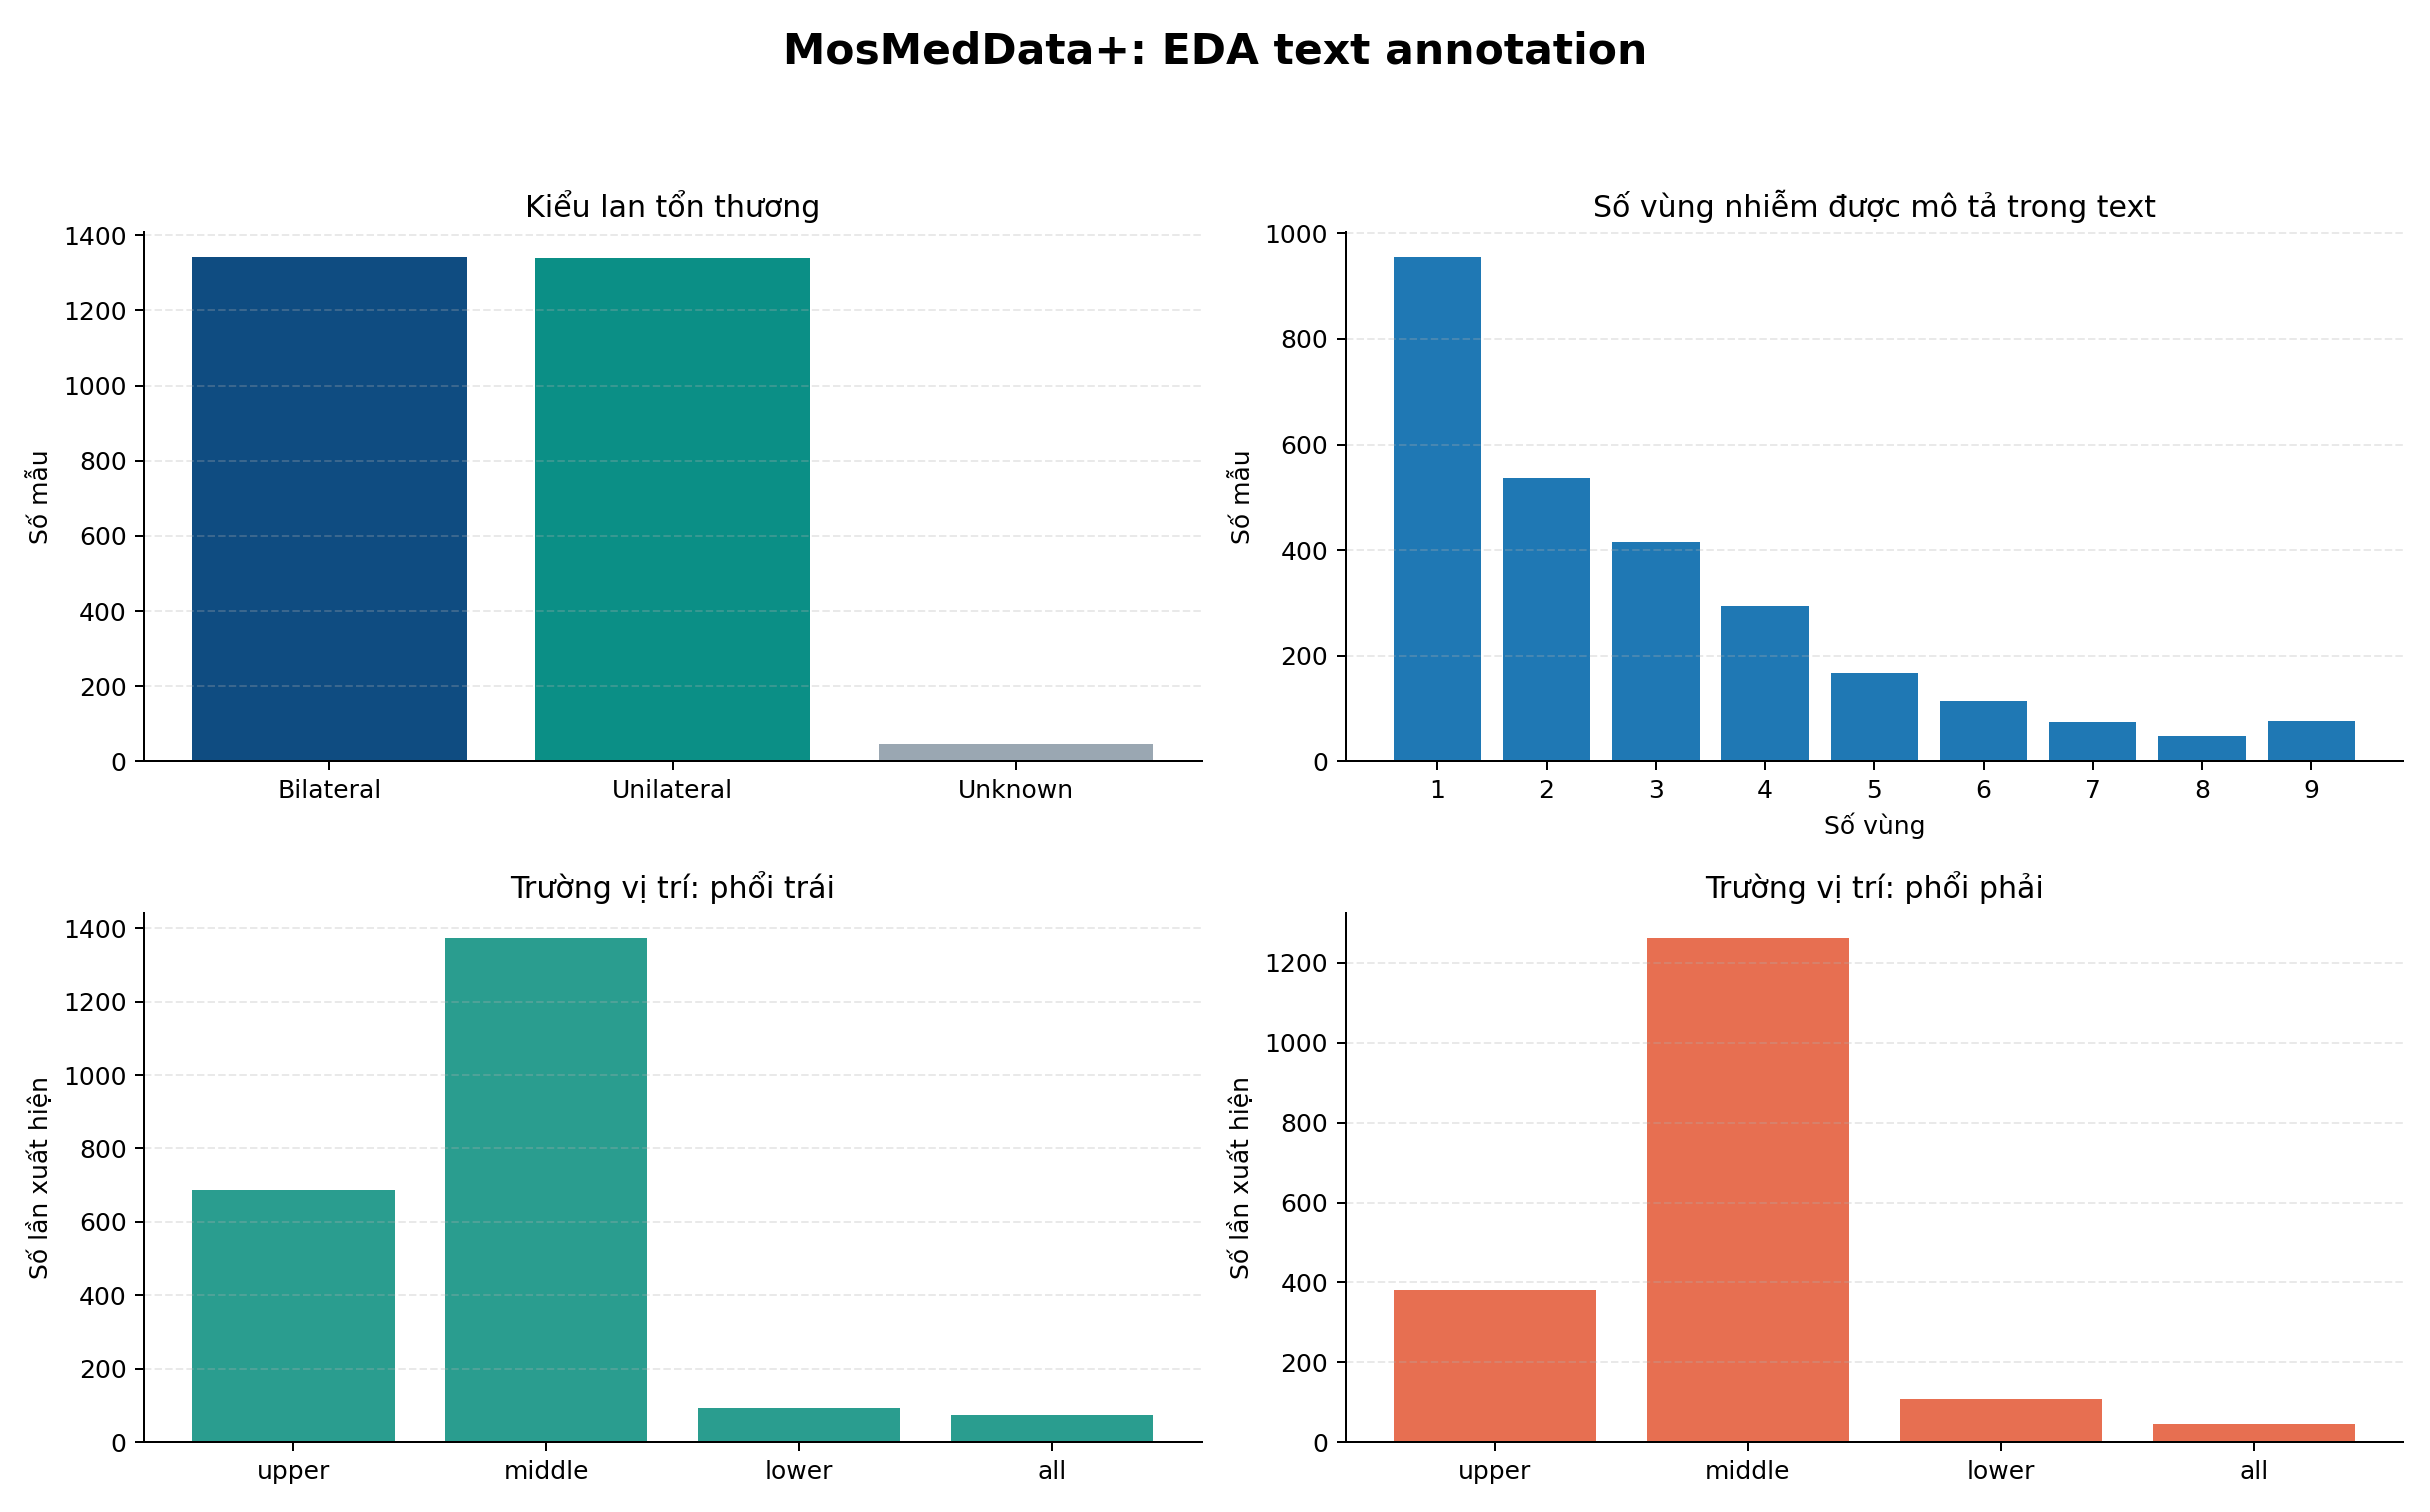
\includegraphics[width=\textwidth]{figures/dataset_text_eda_mosmeddata.png}
  \caption{EDA văn bản chú thích của MosMedData+. So với QaTa-COV19, số vùng nhiễm đa dạng hơn và phân bố unilateral/bilateral gần cân bằng hơn.}
  \label{fig:dataset-văn bản-eda-mosmeddata}
\end{figure}

\begin{table}[H]
  \centering
  \caption{Các trường thông tin có thể tách từ văn bản chú thích của hai bộ dữ liệu.}
  \label{tab:văn bản-chú thích-fields}
  \small
  \renewcommand{\arraystretch}{1.15}
  \setlength{\tabcolsep}{4pt}
  \begin{tabularx}{\textwidth}{@{}p{0.18\textwidth} p{0.22\textwidth} X@{}}
    \toprule
    Bộ dữ liệu & Trường thông tin & Giá trị/ý nghĩa thường gặp \\
    \midrule
    QaTa-COV19 & Kiểu lan tổn thương & Unilateral hoặc bilateral pulmonary infection; cho biết tổn thương một bên hay hai bên phổi. \\
    QaTa-COV19 & Số vùng nhiễm & One đến six infected areas trong gói dữ liệu phân tích; đa số là two infected areas. \\
    QaTa-COV19 & Vị trí trái/phải & Left lung, right lung kết hợp với upper, middle, lower, all; mô tả vị trí tương đối trên X-quang. \\
    MosMedData+ & Nguồn ảnh & Morozov/MosMedData, Jun/Coronacases--Radiopaedia, Bjørke/MedSeg CT; phản ánh dữ liệu CT được gộp từ nhiều nguồn. \\
    MosMedData+ & Kiểu lan và số vùng & Unilateral/bilateral và one đến nine infected areas; số vùng đa dạng hơn QaTa-COV19. \\
    MosMedData+ & Vị trí trái/phải & Upper/middle/lower/all left/right lung; thường tập trung vào middle lung trong gói phân tích. \\
    \bottomrule
  \end{tabularx}
\end{table}
\FloatBarrier

Trong phần thực nghiệm, các thử nghiệm tập trung vào QaTa-COV19 ở các tỉ lệ nhãn 25\%, 50\%, 100\%, và mở rộng sang MosMedData+ ở 50\% nhãn. Dữ liệu được tổ chức theo dạng LViT: mỗi split có ảnh, mặt nạ và bảng văn bản chứa định danh mẫu cùng mô tả tương ứng. Cách tổ chức này giúp báo cáo vừa bám paper gốc, vừa giải thích được cách hệ thống dùng \(x,t,y\) khi tái hiện hoặc mở rộng.

\subsection{Framework chung của hệ thống}

Framework chung của một hệ thống kiểu LViT có thể chia thành sáu khối xử lý chính. Các khối này chưa bắt buộc phải dùng đúng module cụ thể của LViT; chúng mô tả những việc mô hình phải làm sau khi dữ liệu đã được chuẩn bị theo dạng \((x,t,y)\) hoặc \((x,t)\). Vì vậy, phần chuẩn bị dữ liệu như đồng bộ định danh mẫu, resize ảnh, đọc bảng văn bản hay chia tập có nhãn/chưa nhãn được xem là tiền xử lý dữ liệu, không phải một module trong khung hệ thống mô hình.

\begin{figure}[H]
  \centering
  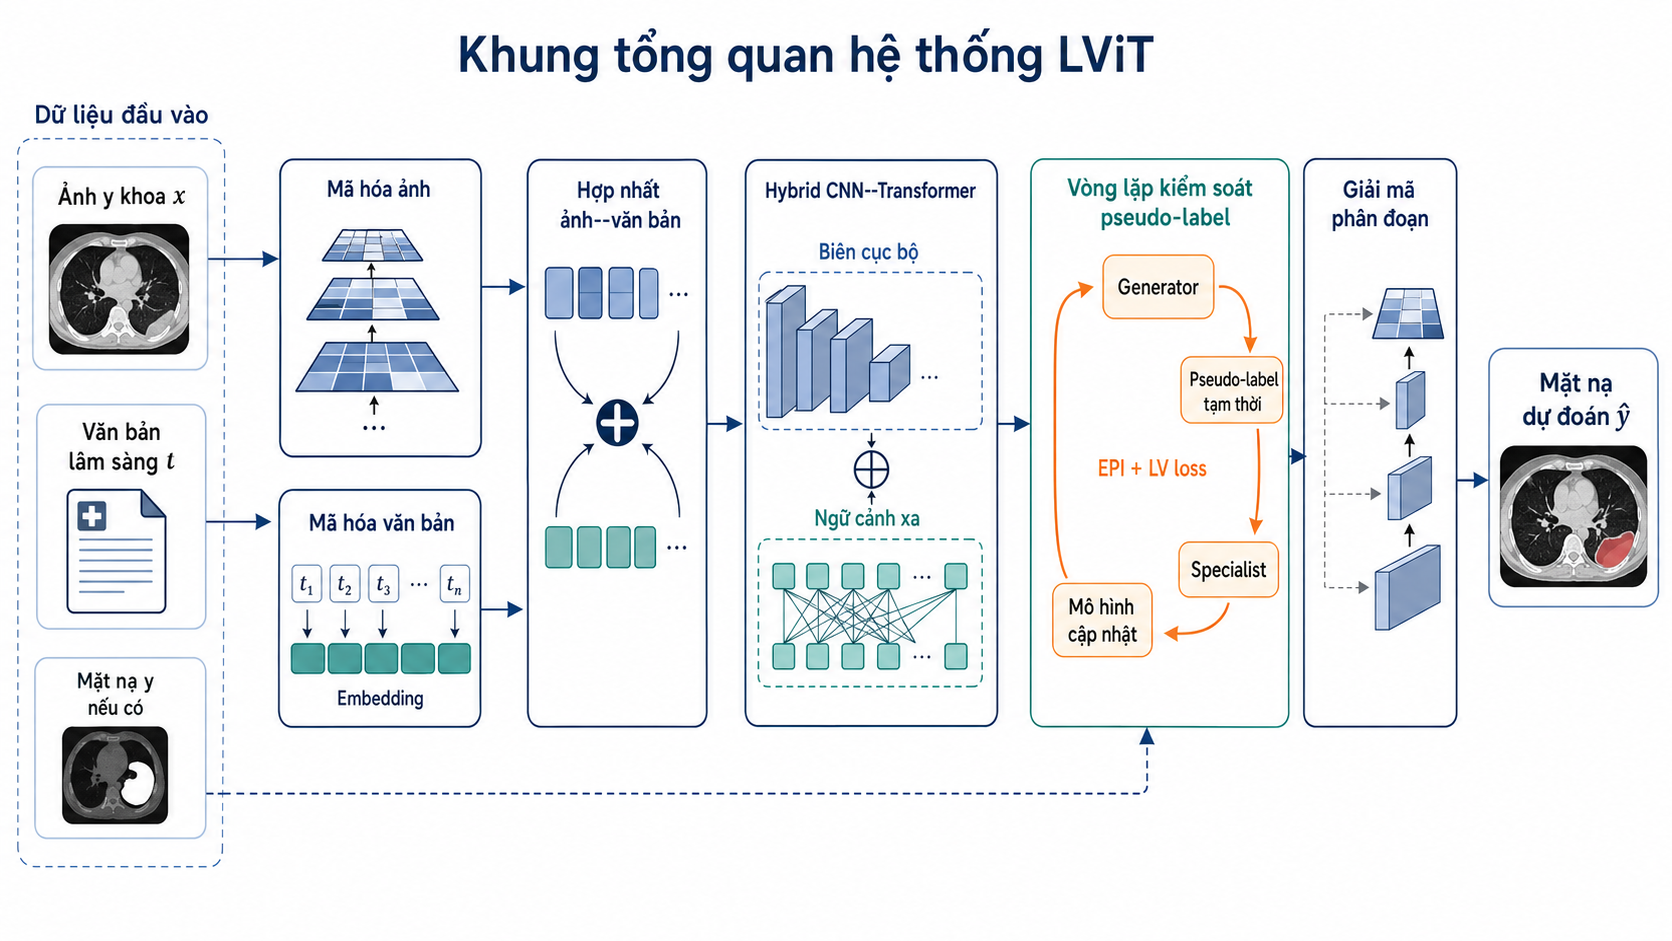
\includegraphics[width=\textwidth]{figures/lvit_system_overview_generated.png}
  \caption{Khung tổng quan hệ thống LViT ở mức module. Dữ liệu đầu vào gồm ảnh, văn bản và mặt nạ nếu có; các khối xử lý chính gồm mã hóa ảnh, mã hóa văn bản, hợp nhất ảnh--văn bản, khối lai CNN--Transformer, vòng lặp kiểm soát pseudo-label và giải mã phân đoạn.}
  \label{fig:lvit-system-overview}
\end{figure}

Hình \ref{fig:lvit-system-overview} cần được đọc từ trái sang phải. Khối dữ liệu đầu vào chỉ mô tả các nguồn thông tin có thể có của một mẫu, không phải một bước xử lý trong mô hình. Ảnh \(x\) đi vào nhánh xử lý ảnh để rút trích thông tin không gian; văn bản \(t\) đi vào nhánh xử lý ngôn ngữ để rút trích ngữ nghĩa mô tả; mặt nạ \(y\), nếu có, chỉ đóng vai trò nhãn xác thực trong học có giám sát hoặc làm chuẩn đối chiếu khi đánh giá. Sau đó, thông tin ảnh và văn bản được đưa vào cùng một pipeline để hình thành mặt nạ dự đoán \(\hat{y}\).

Ở mức khung bài toán, phần ``Hybrid CNN--Transformer'' trong hình không nên được hiểu như một kiến trúc bắt buộc, mà như một công đoạn mô hình hóa đặc trưng. Bản chất của công đoạn này là hệ thống phải đồng thời giữ được chi tiết cục bộ của ảnh và nắm được ngữ cảnh xa hoặc ngữ nghĩa toàn cục. Một số phương pháp giải quyết bằng CNN thuần, một số bằng Transformer thuần, và một số bằng mô hình lai. Vì vậy, ở Chương 1 chỉ cần xác định rằng bài toán cần một cơ chế học biểu diễn vừa nhạy với biên, vừa đủ mạnh để khai thác bối cảnh rộng và tín hiệu văn bản.

Tương tự, khối ``kiểm soát pseudo-label'' trong hình không nên bị đồng nhất với một kỹ thuật cụ thể. Về bản chất, đây là công đoạn dành cho dữ liệu chưa có mặt nạ thật: hệ thống phải tự tạo ra mục tiêu tạm thời từ dự đoán hiện tại, đồng thời có cơ chế kiểm soát độ tin cậy của mục tiêu đó trước khi học tiếp. Công đoạn này có thể được hiện thực bằng nhiều hướng như nhãn giả, consistency regularization, teacher--student, hoặc ràng buộc phụ từ văn bản. Điểm quan trọng ở mức framework là phải chỉ ra sự tồn tại của vòng lặp ``dự đoán tạm thời -- kiểm soát -- học lại'', chứ chưa khóa vào một công thức cụ thể.

\begin{enumerate}
  \item \textbf{Mã hóa ảnh.} Ảnh đầu vào cần được chuyển thành các bản đồ đặc trưng đa mức: tầng nông giữ biên, texture và chi tiết cục bộ; tầng sâu giữ ngữ nghĩa và bối cảnh rộng hơn. Ẩn số cần học ở đây là các tham số của bộ trích đặc trưng ảnh.

  \item \textbf{Mã hóa văn bản.} Văn bản lâm sàng cần được biến thành token, vector hoặc embedding để có thể được máy học xử lý. Ẩn số cần học ở công đoạn này là các tham số của bộ mã hóa ngôn ngữ hoặc các phép chiếu đưa văn bản về không gian biểu diễn phù hợp với ảnh.

  \item \textbf{Hợp nhất ảnh--văn bản.} Sau khi có đặc trưng ảnh và đặc trưng văn bản, hệ thống phải quyết định văn bản sẽ tác động lên biểu diễn ảnh ở đâu và bằng cách nào. Ẩn số cần học ở đây là các tham số của cơ chế fusion, chẳng hạn trọng số chú ý, phép chiếu, cổng điều biến hoặc hàm tổng hợp biểu diễn chung.

  \item \textbf{Mô hình hóa đặc trưng cục bộ và ngữ cảnh xa.} Công đoạn này giúp hệ thống vừa giữ được chi tiết không gian ở mức biên, vừa học được quan hệ xa hoặc bối cảnh toàn cục. Ẩn số cần học là các tham số mô hình hóa ngữ cảnh và truyền thông tin giữa các mức đặc trưng.

  \item \textbf{Tạo và kiểm soát mục tiêu tạm thời cho dữ liệu chưa nhãn.} Khi mẫu chưa có \(y\), hệ thống cần tạo ra một mục tiêu học tạm thời như pseudo-label hoặc tín hiệu consistency, rồi kiểm soát độ tin cậy của nó trước khi dùng để cập nhật mô hình. Ẩn số cần tìm ở đây gồm pseudo-label \(\tilde{y}\), độ tin cậy của pseudo-label hoặc trọng số gán cho các vùng dự đoán.

  \item \textbf{Giải mã và sinh mặt nạ phân đoạn.} Công đoạn cuối cùng biến đặc trưng đã hợp nhất thành bản đồ xác suất mức điểm ảnh, rồi tạo mặt nạ dự đoán \(\hat{y}\). Ẩn số cần học là các tham số của bộ giải mã và lớp dự đoán cuối.
\end{enumerate}

\begin{table}[H]
  \centering
  \caption{Các công đoạn trong khung hệ thống và vai trò của LViT.}
  \label{tab:problem-khung hệ thống}
  \small
  \renewcommand{\arraystretch}{1.15}
  \setlength{\tabcolsep}{3pt}
  \begin{tabularx}{\textwidth}{@{}p{0.24\textwidth} X X@{}}
    \toprule
    Công đoạn & Ẩn số/đầu ra trung gian cần tìm & Cách LViT hiện thực \\
    \midrule
    Mã hóa ảnh & bản đồ đặc trưng cục bộ và đa mức & CNN, U-Net hoặc backbone thị giác khác \\
    Mã hóa văn bản & Token/vector văn bản & embedding, RNN, Transformer encoder hoặc bộ mã hóa ngôn ngữ khác \\
    Fusion ảnh--văn bản & Biểu diễn chung ảnh--văn bản & attention, cross-attention, gating, concatenation hoặc phép chiếu chung \\
    Mô hình hóa cục bộ và ngữ cảnh xa & Đặc trưng vừa giữ biên vừa có bối cảnh rộng & CNN thuần, Transformer thuần hoặc mô hình lai \\
    Kiểm soát mục tiêu tạm thời & Pseudo-label \(\tilde{y}\), độ tin cậy, trọng số học trên mẫu chưa nhãn & pseudo-label, consistency, teacher--student hoặc ràng buộc phụ từ văn bản \\
    Phân đoạn & Mặt nạ xác suất \(\hat{y}\) & bộ giải mã phân đoạn và lớp dự đoán cuối \\
    \bottomrule
  \end{tabularx}
\end{table}
\FloatBarrier

\subsection{Phần dùng pretrained và phần học từ đầu}

Một điểm dễ nhầm trong bài toán này là xem mọi thành phần đều được pretrained. Thực tế cần tách rõ. Trong LViT gốc, thành phần văn bản dùng BERT-Embed pretrained để có vector từ 768 chiều; đây là tri thức ngôn ngữ học được từ tập văn bản lớn trước đó. Tuy nhiên, LViT không lấy nguyên một mô hình vision-language lớn đã học sẵn để phân đoạn y khoa. Các khối CNN, ViT đa mức, PLAM, bộ giải mã và cơ chế tương tác ảnh--văn bản vẫn được huấn luyện cho nhiệm vụ phân đoạn trên các tập đích.

Trong phần mở rộng, nếu dùng BiomedBERT thì phần bộ mã hóa văn bản được lấy từ mô hình pretrained trên văn bản y sinh và có thể lưu trước đặc trưng để tiết kiệm thời gian chạy. Phần này giúp biến báo cáo thành embedding có ngữ cảnh y sinh tốt hơn. Nhưng những khối quyết định mặt nạ như fusion, bộ giải mã, pseudo-label control và loss vẫn phải học từ dữ liệu phân đoạn cụ thể như QaTa-COV19 hoặc MosMedData+. Nói cách khác, pretrained bộ mã hóa văn bản cung cấp ngôn ngữ nền; còn năng lực khoanh vùng tổn thương không tự xuất hiện từ pretrained, mà được học nhờ ảnh, mask và quá trình tối ưu.

Các ẩn số phải tìm trong toàn bộ khung hệ thống gồm: tham số mã hóa ảnh, tham số chuyển đổi/mã hóa văn bản, trọng số fusion ảnh--văn bản, trọng số của khối CNN--Transformer, tham số bộ giải mã sinh mặt nạ, và trong bán giám sát là pseudo-label hoặc độ tin cậy của pseudo-label. Cách xác định các ẩn số này có thể khác nhau giữa CNN thuần, Transformer thuần, mô hình lai hoặc mô hình vision-language; LViT là một lời giải cụ thể trong không gian đó, nổi bật vì nó đưa văn bản vào cả biểu diễn đặc trưng lẫn kiểm soát pseudo-label.

\section{Đóng góp của báo cáo}

Đóng góp của báo cáo cần được hiểu theo hai lớp. Lớp thứ nhất, và cũng là trọng tâm chính, là khảo sát LViT như một phương pháp đã công bố: đọc paper, đối chiếu với triển khai chính thức, giải thích lại bài toán và phương pháp theo cách tự đủ hiểu. Lớp thứ hai là phần thực hành mở rộng: tái hiện, đặc tả, phân tích dữ liệu và thử nghiệm một số cải tiến có kiểm soát. Điểm cần nhấn mạnh ngay từ đầu là các cải tiến này không chỉ dừng ở mức ý tưởng kiến trúc, mà đã được kiểm tra sơ bộ trên QaTa-COV19: khi tăng tỉ lệ dữ liệu có nhãn từ 25\%, 50\% đến 100\%, mô hình cải tiến đạt Dice kiểm thử lần lượt khoảng \(82.22\%\), \(84.03\%\) và \(85.28\%\); IoU kiểm thử lần lượt khoảng \(73.35\%\), \(75.62\%\) và \(77.25\%\). Vì vậy, báo cáo vừa giải thích LViT gốc, vừa dùng kết quả cải tiến để cho thấy hướng mở rộng ảnh--văn bản và bán giám sát là có cơ sở thực nghiệm. Cách tách này quan trọng vì báo cáo vẫn tập trung vào LViT của Li et al.; các cải tiến được trình bày như phần đóng góp bổ sung để hiểu và kiểm chứng phương pháp, không thay thế đóng góp gốc của bài báo.

Cụ thể, báo cáo đóng góp các nội dung sau:
\begin{itemize}
  \item \textbf{Đặc tả bài toán phân đoạn ảnh--văn bản theo khung hệ thống chung.} Báo cáo tách rõ dữ liệu đầu vào, đầu ra, ground truth và các ẩn số cần học. Khung hệ thống được trình bày ở mức công đoạn thay vì nhảy ngay vào kiến trúc LViT, giúp người đọc thấy nhiều lựa chọn phương pháp có thể tồn tại trong từng công đoạn: mã hóa ảnh, mã hóa văn bản, fusion, học ngữ cảnh xa, kiểm soát pseudo-label và giải mã phân đoạn.

  \item \textbf{Giải thích LViT theo hướng tự đủ hiểu.} Báo cáo không chỉ liệt kê tên module, mà giải thích vì sao LViT cần Double-U, vì sao CNN giữ tốt chi tiết cục bộ, vì sao Transformer/self-attention học được ngữ cảnh xa, vì sao văn bản có thể hỗ trợ phân đoạn và vì sao pseudo-label cần được kiểm soát lặp lại bằng EPI và LV loss \cite{li2023lvit}. Mục tiêu là người đọc không cần biết sâu trước về CNN, Transformer hay vision-language model vẫn có thể theo được logic chính.

  \item \textbf{Phân tích dữ liệu và văn bản chú thích của LViT.} Báo cáo khảo sát hai bộ dữ liệu chính gồm QaTa-COV19 và MosMedData+; tạo lưới cặp ảnh--văn bản; phân tích cấu trúc văn bản chú thích; và vẽ EDA cho các trường như kiểu lan tổn thương, số vùng nhiễm, vị trí trái/phải, vùng upper/middle/lower/all và nguồn con của MosMedData+. Phần này làm rõ văn bản trong LViT là tín hiệu có cấu trúc chứ không phải một chuỗi tự do hoàn toàn.

  \item \textbf{Tổng hợp related works theo cùng tiêu chí so sánh.} Các hướng CNN, Transformer, mô hình lai CNN--Transformer, vision-language learning và học bán giám sát sẽ được đặt vào cùng các tiêu chí gắn với khung hệ thống ở mục 1.3. Nhờ đó, chương 2 không trình bày mỗi công trình theo một dàn bài riêng, mà trả lời được hai câu hỏi: người ta đã làm gì rồi, và LViT muốn giải quyết phần nào còn thiếu.

  \item \textbf{Đối chiếu paper với triển khai chính thức.} Báo cáo sử dụng triển khai chính thức của HUANGLIZI/LViT để mô tả cách hệ thống tổ chức dữ liệu, mô hình, huấn luyện và đánh giá \cite{lvitOfficialRepo}. Phần này giúp người đọc hiểu LViT không chỉ ở mức sơ đồ paper, mà còn ở mức vận hành: dữ liệu ảnh--văn bản--mask được đưa vào mô hình như thế nào, module nào tương ứng với kiến trúc, và quá trình học/kiểm thử đi qua các bước nào.

  \item \textbf{Thực hiện phần cải tiến và mở rộng, đồng thời báo cáo kết quả đạt được.} Bên cạnh việc bám LViT gốc, báo cáo thử nghiệm các cải tiến nhằm khảo sát hướng phát triển của LViT. Về kết quả, mô hình cải tiến cho xu hướng tăng ổn định khi có thêm dữ liệu có nhãn: trên QaTa-COV19, cấu hình 25\% nhãn đạt khoảng \(80.11\%\) Dice validation và \(82.22\%\) Dice test; cấu hình 50\% nhãn đạt khoảng \(81.56\%\) Dice validation và \(84.03\%\) Dice test; cấu hình 100\% nhãn đạt khoảng \(82.95\%\) Dice validation và \(85.28\%\) Dice test. IoU test cũng tăng tương ứng từ \(73.35\%\) lên \(75.62\%\) và \(77.25\%\). Điều này cho thấy cải tiến không chỉ nhằm làm mô hình phức tạp hơn, mà hướng đến ba hiệu quả cụ thể: biểu diễn văn bản y sinh tốt hơn, hợp nhất ảnh--văn bản rõ hơn, và kiểm soát nhãn giả ổn định hơn trong bối cảnh ít nhãn.

  Về kỹ thuật, các cải tiến gồm: dùng BiomedBERT/cache embedding để tăng chất lượng biểu diễn văn bản y sinh; bổ sung bottleneck cross-attention để tạo tương tác ảnh--văn bản rõ hơn ở tầng ngữ nghĩa; dùng văn bản spatial prior để biến tóm tắt văn bản thành gợi ý không gian thô; thêm cross-modal skip adapter để điều chỉnh skip features khi giải mã; dùng prototype memory/fallback khi văn bản thiếu hoặc kém tin cậy; và tổ chức lại phần huấn luyện bán giám sát với cơ chế fusion pseudo-label có xét độ không chắc chắn, consistency loss, boundary consistency và prototype alignment. Các cải tiến này được trình bày như phần mở rộng thực nghiệm của báo cáo, cần được so sánh công bằng với LViT gốc ở chương cài đặt/thử nghiệm.
\end{itemize}

Tóm lại, đóng góp của báo cáo không phải là ``phát minh lại'' LViT, mà là làm cho LViT trở nên có thể đọc, có thể hiểu, có thể tái hiện và có thể phân tích tiếp. Phần cải tiến đóng vai trò điểm cộng kỹ thuật: nó cho thấy từ khung hệ thống của LViT có thể đặt ra các hướng mở rộng cụ thể, nhưng trọng tâm học thuật của báo cáo vẫn là phương pháp LViT và ý nghĩa của việc đưa văn bản vào phân đoạn ảnh y khoa.

\chapter{Các công trình nghiên cứu liên quan}
\label{sec:related}

Chương này trả lời hai câu hỏi: người ta đã làm gì rồi, và vì sao LViT là một hướng đáng khảo sát. Cách trình bày không đi theo từng bài một cách rời rạc, mà đi theo quá trình phát triển của các công đoạn trong khung hệ thống: biểu diễn ảnh, biểu diễn ngữ cảnh xa, hợp nhất văn bản và học khi ít nhãn. Nhờ vậy, mỗi công trình được đặt vào đúng vai trò của nó trong hệ thống phân đoạn.

\section{Các phương thức tiếp cận trong phân đoạn ảnh y khoa có văn bản}

Trước khi đi vào từng công trình cụ thể, cần xác định bản đồ các hướng tiếp cận. Một chương related works tốt không chỉ kể tên mô hình, mà phải cho thấy các mô hình đó trả lời phần nào của bài toán. Với LViT, bài toán không còn là phân đoạn ảnh đơn thuần; nó nằm ở giao điểm của phân đoạn y khoa, học ngữ cảnh xa, học đa phương thức ảnh--văn bản và học bán giám sát. Vì vậy, mục này đóng vai trò như phần ``định trục'': phân loại các hướng chính, nêu tiêu chí đánh giá, và chỉ ra những thách thức dữ liệu làm cho LViT trở nên có ý nghĩa.

\begin{figure}[H]
  \centering
  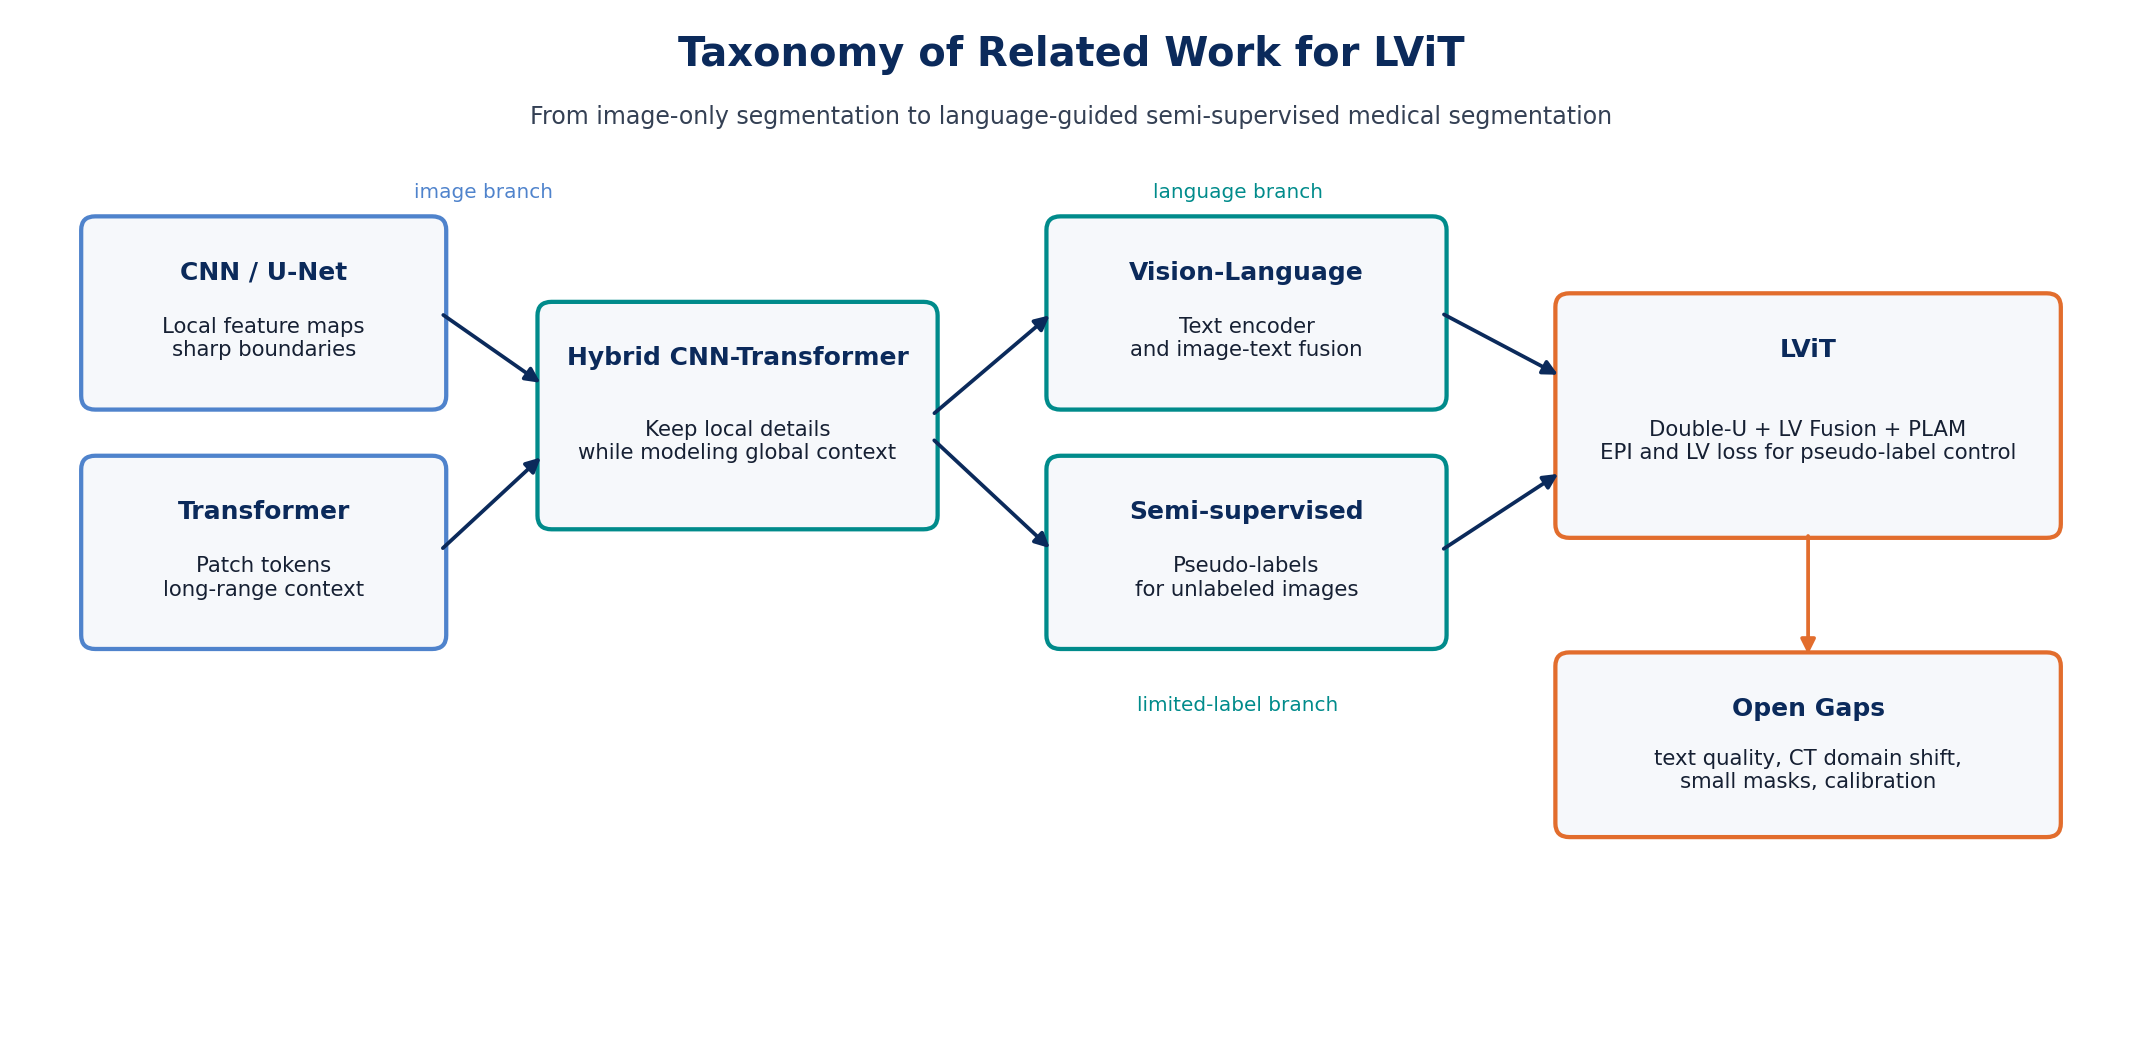
\includegraphics[width=0.95\textwidth]{figures/related_taxonomy_lvit.png}
  \caption{Bản đồ các nhóm công trình liên quan đến LViT. CNN/U-Net giải quyết đặc trưng cục bộ và biên; Transformer giải quyết ngữ cảnh xa; vision-language đưa văn bản vào biểu diễn; học bán giám sát xử lý thiếu mask; LViT kết nối các nhánh này trong một pipeline phân đoạn ảnh y khoa.}
  \label{fig:related-taxonomy-lvit}
\end{figure}

\subsection{Phân loại các hướng phương pháp}

Có thể chia các phương pháp liên quan đến LViT thành năm nhóm. Nhóm thứ nhất là \textbf{CNN/bộ mã hóa--bộ giải mã}, tiêu biểu bởi FCN, U-Net, DeepLab và các biến thể U-Net. Nhóm này xem ảnh như bản đồ đặc trưng, dùng convolution để học đặc trưng cục bộ và bộ giải mã để khôi phục mặt nạ. Đây là nền tảng quan trọng nhất cho biên và cấu trúc không gian.

Nhóm thứ hai là \textbf{attention và Transformer}. Nhóm này xem ảnh hoặc bản đồ đặc trưng như tập token, dùng self-attention để học quan hệ xa giữa các vùng. Điểm mạnh là ngữ cảnh toàn cục; điểm yếu là chi phí tính toán và nguy cơ làm yếu thiên kiến cục bộ nếu dùng Transformer thuần.

Nhóm thứ ba là \textbf{mô hình lai CNN--Transformer}. Nhóm này cố giữ cả hai lợi thế: CNN giữ cục bộ đặc trưng, Transformer học long-range context. Đây là hướng trực tiếp dẫn đến Double-U của LViT.

Nhóm thứ tư là \textbf{vision-language learning}. Nhóm này đưa văn bản vào pipeline thị giác, từ căn chỉnh ảnh--văn bản toàn cục đến văn bản-guided segmentation. Với LViT, văn bản không chỉ là metadata, mà là tín hiệu ngữ nghĩa đi vào đặc trưng/fusion và loss bán giám sát.

Nhóm thứ năm là \textbf{học bán giám sát/pseudo-label}. Nhóm này xử lý tình huống rất phổ biến trong y khoa: có ảnh và có thể có văn bản, nhưng thiếu mask mức điểm ảnh. LViT thuộc nhóm này vì nó dùng EPI và LV loss để kiểm soát nhãn giả trên dữ liệu chưa nhãn.

\begin{table*}[!t]
  \centering
  \caption{Phân loại các hướng tiếp cận liên quan đến LViT theo công đoạn của khung hệ thống.}
  \label{tab:approach-taxonomy}
  \scriptsize
  \renewcommand{\arraystretch}{1.15}
  \setlength{\tabcolsep}{5pt}
  \begin{tabularx}{\textwidth}{@{}l L L L@{}}
    \toprule
    Hướng tiếp cận & Công đoạn chính & Tóm tắt & Thiếu hụt dẫn đến LViT \\
    \midrule
    CNN/U-Net & Mã hóa ảnh, bộ giải mã & bản đồ đặc trưng cục bộ, giữ biên & Thiếu ngữ cảnh xa/văn bản \\
    Transformer & Ngữ cảnh xa & Token và self-attention & Dễ tốn chi phí, yếu cục bộ \\
    CNN--Transformer & Hybrid đặc trưng/token & Kết hợp biên và ngữ cảnh & Chưa khai thác văn bản \\
    Vision-language & bộ mã hóa văn bản, fusion & Đưa ngữ nghĩa vào ảnh & Cần mask mức điểm ảnh \\
    Semi-supervised & Pseudo-label & Học từ ảnh ít mask & Cần kiểm soát nhãn giả \\
    LViT & Toàn pipeline & Ảnh + văn bản + SSL & Phụ thuộc chất lượng văn bản \\
    \bottomrule
  \end{tabularx}
\end{table*}
\FloatBarrier

\subsection{Benchmark và độ đo đánh giá}

Trong phân đoạn y khoa, đánh giá không thể chỉ nhìn loss huấn luyện. Loss là hàm tối ưu trong quá trình học; hiệu suất là cách đo chất lượng mặt nạ sau khi mô hình dự đoán. Hai khái niệm này liên quan nhưng không đồng nhất. Một mô hình có thể tối ưu BCE tốt nhưng vẫn cho biên kém; hoặc Dice loss tốt nhưng vùng nhỏ vẫn bị bỏ sót. Vì vậy, related works cần so sánh bằng cùng nhóm độ đo, tránh việc mỗi công trình được kể bằng một tiêu chí khác nhau.

Các độ đo thường gặp gồm Dice, IoU/mIoU, precision, recall và đôi khi có Hausdorff distance hoặc boundary-based metric. Dice đo mức chồng lấn giữa mặt nạ dự đoán và ground truth, rất phổ biến khi foreground nhỏ. IoU cũng đo chồng lấn nhưng thường nghiêm hơn Dice vì mẫu số tính theo hợp hai vùng. Precision cho biết vùng dự đoán dương có bao nhiêu phần đúng; recall cho biết vùng thật được bắt lại bao nhiêu. Với ảnh y khoa, recall thấp có thể nguy hiểm vì bỏ sót tổn thương, còn precision thấp làm mask nhiễu và có thể gây hiểu nhầm.

Bên cạnh độ chính xác, cần xem \textbf{độ phức tạp tính toán}. Một mô hình dùng Transformer và văn bản branch thường có nhiều tham số, FLOPs và bộ nhớ hơn U-Net thuần. Vì vậy, khi nói LViT cải thiện Dice/IoU, báo cáo cũng cần bàn luận chi phí đổi lại: bộ mã hóa văn bản, attention đa mức, PLAM, pseudo-label loop và thời gian huấn luyện. Đây là điểm dàn ý mẫu nhấn mạnh rất đúng: hiệu suất không chỉ là accuracy, mà còn là chi phí để đạt accuracy đó.

\subsection{Công tác dữ liệu và challenges}

Trong phân đoạn y khoa, dữ liệu quyết định rất mạnh giá trị của kết quả. Nếu tập dữ liệu ít ca khó, ít biến thiên, hoặc ground truth được đánh nhãn không nhất quán, hiệu suất cao chưa chắc chứng minh phương pháp tốt. Với LViT, công tác dữ liệu còn phức tạp hơn vì mỗi mẫu có thể gồm ba phần: ảnh \(x\), văn bản \(t\) và mặt nạ \(y\). Ba phần này phải khớp nhau về định danh mẫu, ca bệnh, lát cắt và ý nghĩa lâm sàng.

\subsubsection{Tính chủ quan của ground truth}

Mask y khoa thường cần bác sĩ hoặc chuyên gia vẽ thủ công. Biên tổn thương có thể mờ, vùng bất thường có thể chuyển tiếp mềm, và hai chuyên gia có thể vẽ hơi khác nhau. Điều này làm ground truth không phải một chân lý tuyệt đối, mà là chuẩn xác thực tốt nhất có được trong điều kiện thực tế. Khi đọc kết quả Dice/IoU, cần nhớ rằng một phần sai khác ở biên có thể đến từ chính độ mơ hồ khi đánh nhãn, không chỉ do mô hình kém.

\subsubsection{Phương pháp thu thập ground truth và văn bản chú thích}

Ground truth \(y\) được thu thập bằng cách khoanh vùng mức điểm ảnh, trong khi văn bản chú thích \(t\) thường được chuẩn hóa từ mô tả lâm sàng hoặc chú thích đi kèm ảnh. Hai loại nhãn này khác bản chất: \(y\) là giám sát không gian chi tiết, còn \(t\) là giám sát ngữ nghĩa thô hơn. Văn bản có thể ghi vùng tổn thương, mức độ hoặc kết luận, nhưng nó thường không chỉ ra ranh giới điểm ảnh. Vì vậy, văn bản hữu ích để bổ sung ngữ nghĩa, nhưng không thể thay thế \(y\). Đây là lý do LViT cần fusion và LV loss thay vì chỉ dùng văn bản như nhãn phân loại.

\subsubsection{Challenges trong data quality}

QaTa-COV19 là X-quang ngực, còn MosMedData+ là CT ngực. Hai loại ảnh này khác nhau về cường độ, cấu trúc không gian, trường nhìn, mức nhiễu và cách đánh nhãn. Một phương pháp tốt cần được hiểu trong bối cảnh từng tập, không nên gộp mọi kết quả thành một nhận xét chung chung. Ngoài ra, khi chỉ một phần dữ liệu có mask, mô hình phải học từ tập chưa nhãn. Nhưng pseudo-label có thể sai, và sai số có thể tự khuếch đại qua nhiều vòng huấn luyện. Vì vậy, challenges dữ liệu không chỉ nằm ở việc có bao nhiêu ảnh, mà còn ở việc ảnh--văn bản--mask có khớp nhau không, pseudo-label được tạo ra sao, và độ tin cậy của từng nguồn thông tin được kiểm soát như thế nào.

\section{State-of-the-Art Methods}

Phần này chọn các nhóm công trình tiêu biểu để trình bày theo cùng một logic: nguyên lý cốt lõi, cách thực hiện, công tác dữ liệu/ground truth, hiệu suất hoặc đóng góp, và hạn chế. Cách viết này giúp so sánh các phương pháp theo cùng tiêu chí, thay vì mỗi bài được kể bằng một dàn ý khác nhau. Các phương pháp được chọn không nhằm bao phủ toàn bộ lịch sử segmentation, mà nhằm dẫn dắt trực tiếp đến câu hỏi của LViT: vì sao cần vừa giữ chi tiết cục bộ, vừa học ngữ cảnh xa, vừa khai thác văn bản, vừa kiểm soát nhãn giả khi thiếu mask.

\begin{table*}[!t]
  \centering
  \caption{Bảng đọc nhanh các công trình tiêu biểu dẫn đến LViT.}
  \label{tab:sota-quick-map}
  \scriptsize
  \renewcommand{\arraystretch}{1.15}
  \setlength{\tabcolsep}{5pt}
  \begin{tabularx}{\textwidth}{@{}l L L L@{}}
    \toprule
    Công trình & Vai trò trong luồng & Đóng góp/hiệu suất & Hạn chế \\ 
    \midrule
    U-Net \cite{ronneberger2015unet} & Mã hóa--giải mã ảnh & Chuẩn mạnh cho segmentation y khoa ít dữ liệu & Thiếu ngữ cảnh xa/văn bản \\
    nnU-Net \cite{isensee2021nnunet} & Pipeline thực nghiệm & Tự cấu hình tiền xử lý, train, hậu xử lý & Không khai thác văn bản \\
    TransUNet \cite{chen2021transunet} & CNN + Transformer & Kết hợp chi tiết cục bộ và ngữ cảnh xa & Đơn phương thức ảnh \\
    Swin-Unet \cite{cao2021swinunet} & Window attention & Giảm chi phí attention trong segmentation & Phụ thuộc thiết kế cửa sổ \\
    ConVIRT/GLoRIA \cite{zhang2020convirt,huang2021gloria} & Ảnh--báo cáo y khoa & Chứng minh văn bản hỗ trợ học biểu diễn y khoa & Chưa trực tiếp sinh mask \\
    Mean Teacher/DTC \cite{tarvainen2017meanteacher,luo2021dtc} & Học bán giám sát & Tận dụng dữ liệu chưa có mask & Pseudo-label dễ nhiễu \\
    LViT \cite{li2023lvit} & Ảnh + văn bản + SSL & Double-U, PLAM, LV Fusion, EPI/LV loss & Phụ thuộc chất lượng văn bản \\
    \bottomrule
  \end{tabularx}
\end{table*}
\FloatBarrier

\subsection{U-Net như đại diện nhóm CNN encoder--decoder}

Trong nhóm phương pháp dựa trên CNN, báo cáo chọn U-Net làm công trình đại diện chính vì đây là kiến trúc có ảnh hưởng sâu nhất đến phân đoạn y khoa hiện đại. FCN và DeepLab vẫn được nhắc đến như các mốc nền tảng dẫn đường, còn UNet++, Attention U-Net và nnU-Net được xem là các nhánh mở rộng xoay quanh cùng một triết lý bộ mã hóa--bộ giải mã.

\subsubsection{Nguyên lý}

Hướng CNN có thể xem là nền móng của phân đoạn ảnh y khoa hiện đại. Triết lý của nhóm phương pháp này là ảnh chứa nhiều mẫu cục bộ có ý nghĩa: cạnh mô, vùng sáng/tối bất thường, texture của tổn thương, ranh giới giữa cơ quan và nền. Convolution khai thác giả định đó bằng cách dùng cùng một kernel trượt trên toàn ảnh, nhờ vậy mô hình học được các bộ phát hiện đặc trưng lặp lại ở nhiều vị trí. Với ảnh y khoa, giả định cục bộ này rất quan trọng vì mặt nạ phân đoạn thường được quyết định bởi biên giải phẫu và thay đổi cường độ tại vùng lân cận. Tuy nhiên, chỉ nhìn cục bộ là chưa đủ: một vùng mờ nhỏ trong phổi hoặc một tổn thương sát biên cơ quan thường cần được hiểu trong ngữ cảnh rộng hơn.

Trong khung hệ thống ở mục 1.3, nhóm CNN chủ yếu giải quyết hai công đoạn: \textit{mã hóa ảnh} và \textit{giải mã phân đoạn}. Đầu vào là ảnh \(x\), đầu ra là mặt nạ dự đoán \(\hat{y}\), còn ground truth \(y\) được dùng để tối ưu loss theo điểm ảnh. Nhóm này thường không dùng văn bản \(t\), không có module fusion ảnh--văn bản và cũng không trực tiếp kiểm soát pseudo-label bằng ngôn ngữ. Vì vậy, CNN là điểm xuất phát tốt để hiểu LViT: LViT không phủ nhận CNN, mà giữ CNN như phần học đặc trưng cục bộ rồi bổ sung Transformer và văn bản chú thích để xử lý những phần CNN còn yếu.

\subsubsection{Phương pháp}

\textbf{FCN: chuyển phân loại ảnh thành dự đoán dày đặc.} Fully Convolutional Network (FCN) là một bước ngoặt vì nó thay các tầng fully-connected của mạng phân loại bằng các tầng convolution, cho phép mô hình sinh bản đồ dự đoán theo từng điểm ảnh thay vì chỉ sinh một nhãn ảnh \cite{long2015fcn}. Nói cách khác, FCN biến bài toán từ ``ảnh này thuộc lớp nào'' thành ``mỗi điểm ảnh trong ảnh thuộc lớp nào''. Nguyên lý này rất gần với phân đoạn y khoa: mô hình phải quyết định từng điểm ảnh là tổn thương, cơ quan hay nền. FCN cũng dùng upsampling để đưa bản đồ đặc trưng độ phân giải thấp trở lại kích thước gần với ảnh gốc. Đóng góp chính của FCN là đặt nền cho semantic segmentation bằng mạng học sâu end-to-end; hạn chế là kết quả biên thường thô vì nhiều lần pooling làm mất chi tiết không gian.

\textbf{DeepLab: mở rộng trường nhìn và làm sắc biên.} DeepLab cải thiện phân đoạn bằng atrous convolution/dilated convolution, tức là mở rộng khoảng cách lấy mẫu trong kernel để tăng receptive field mà không phải giảm thêm độ phân giải bản đồ đặc trưng \cite{chen2018deeplab}. Điều này có ý nghĩa với ảnh y khoa vì tổn thương có thể cần được nhận biết trong bối cảnh của toàn cơ quan. Một số biến thể DeepLab còn dùng cơ chế tổng hợp đa tỉ lệ và hậu xử lý biên để làm mặt nạ sắc hơn. Đóng góp của DeepLab là cho thấy không chỉ kiến trúc bộ mã hóa--bộ giải mã, mà cách kiểm soát trường nhìn và đa tỉ lệ cũng ảnh hưởng mạnh đến phân đoạn. Hạn chế là phương pháp vẫn dựa chủ yếu vào đặc trưng ảnh, chưa khai thác được thông tin ngoài ảnh như ghi chú lâm sàng.

\textbf{U-Net: bộ mã hóa--bộ giải mã và skip connection cho dữ liệu y khoa ít nhãn.} Trong ảnh y khoa, U-Net trở thành kiến trúc kinh điển vì nó phù hợp với đặc điểm dữ liệu: số lượng mẫu thường ít, nhưng cần dự đoán mặt nạ chính xác ở mức điểm ảnh \cite{ronneberger2015unet}. U-Net có hai nhánh đối xứng. Nhánh bộ mã hóa giảm dần kích thước không gian để học đặc trưng ngữ nghĩa, ví dụ vùng nào có khả năng là phổi, tổn thương hoặc nền giải phẫu. Nhánh bộ giải mã tăng dần kích thước để khôi phục mặt nạ. Điểm quan trọng là skip connection nối bản đồ đặc trưng cùng mức giữa bộ mã hóa và bộ giải mã. Nhờ skip connection, bộ giải mã không phải tự khôi phục chi tiết biên từ bản đồ đặc trưng quá thô, mà nhận lại thông tin cục bộ đã học ở các tầng nông. Đây là lý do U-Net thường giữ biên tốt hơn FCN cơ bản.

Nếu đặt U-Net vào ngôn ngữ của bài toán, bộ mã hóa học ánh xạ \(f_\theta(x)\) từ ảnh sang đặc trưng nhiều mức; bộ giải mã học ánh xạ \(g_\theta(f_\theta(x))\) từ đặc trưng sang mặt nạ \(\hat{y}\). Trong giai đoạn học, \(\hat{y}\) được so với mask \(y\) bằng các loss như cross-entropy, Dice loss hoặc biến thể kết hợp. Loss không phải độ đo đánh giá, nhưng có liên hệ trực tiếp: Dice loss thường được dùng vì Dice score là độ đo phổ biến trong phân đoạn y khoa, đặc biệt khi vùng tổn thương nhỏ hơn nền rất nhiều. Như vậy, U-Net giải quyết tốt phần dựa vào bản đồ đặc trưng của bài toán, nhưng chưa có cơ chế để hiểu câu mô tả lâm sàng hoặc quan hệ xa giữa các vùng ảnh.

\subsubsection{Công tác lựa chọn và làm dữ liệu}

Khi dùng nhóm CNN/U-Net, dữ liệu cần được chuẩn hóa thành cặp ảnh--mặt nạ có cùng kích thước và đúng định danh mẫu. Ảnh thường được đưa về một kích thước cố định, chuẩn hóa cường độ và tăng cường bằng các phép biến đổi không làm sai cấu trúc giải phẫu. Mặt nạ \(y\) là nguồn giám sát chính, nên chất lượng biên và tính nhất quán giữa chuyên gia ảnh hưởng trực tiếp đến Dice/IoU. Nhóm phương pháp này không yêu cầu văn bản, vì vậy nếu tập dữ liệu có văn bản chú thích thì nguồn thông tin đó chưa được khai thác.

\subsubsection{Hiệu suất}

\textbf{Các biến thể của U-Net: cải thiện skip, attention và quy trình huấn luyện.} UNet++ nhận thấy skip connection của U-Net còn tạo ra khoảng cách ngữ nghĩa giữa đặc trưng nông và đặc trưng sâu, nên dùng các skip path lồng nhau để làm giàu đặc trưng trước khi ghép vào bộ giải mã \cite{zhou2018unetpp}. Attention U-Net thêm attention gate để bộ giải mã tập trung hơn vào vùng liên quan và giảm nhiễu từ vùng nền \cite{oktay2018attention}. nnU-Net đi theo hướng khác: thay vì chỉ đề xuất một kiến trúc mới, nó chuẩn hóa toàn bộ pipeline từ tiền xử lý, chọn cấu hình mạng, augmentation, huấn luyện đến hậu xử lý theo từng bộ dữ liệu \cite{isensee2021nnunet}. Đây là đóng góp quan trọng vì trong thực nghiệm y khoa, hiệu suất không chỉ đến từ backbone mà còn đến từ cách chuẩn hóa ảnh, chia dữ liệu, chọn patch size, batch size và chiến lược hậu xử lý.

\begin{table*}[!t]
  \centering
  \caption{Các phương pháp CNN tiêu biểu trong phân đoạn y khoa và liên hệ với khung hệ thống ở mục 1.3.}
  \label{tab:cnn-related-works}
  \scriptsize
  \renewcommand{\arraystretch}{1.15}
  \setlength{\tabcolsep}{5pt}
  \begin{tabularx}{\textwidth}{@{}l L L L@{}}
    \toprule
    Công trình & Trọng tâm & Tóm tắt & Hạn chế \\
    \midrule
    FCN \cite{long2015fcn} & Dense prediction & Dự đoán nhãn từng điểm ảnh end-to-end & Biên thô, thiếu văn bản \\
    DeepLab \cite{chen2018deeplab} & Đa tỉ lệ & Mở rộng receptive field bằng atrous convolution & Vẫn đơn phương thức \\
    U-Net \cite{ronneberger2015unet} & bộ mã hóa--bộ giải mã & Skip connection giữ chi tiết biên & Ngữ cảnh xa gián tiếp \\
    UNet++ \cite{zhou2018unetpp} & Skip cải tiến & Làm giàu đặc trưng trước khi giải mã & Phức tạp hơn U-Net \\
    Attention U-Net \cite{oktay2018attention} & Attention gate & Lọc nhiễu nền khi ghép skip & Attention nội bộ ảnh \\
    nnU-Net \cite{isensee2021nnunet} & Pipeline tự cấu hình & Chuẩn hóa tiền xử lý, train, hậu xử lý & Không khai thác văn bản \\
    \bottomrule
  \end{tabularx}
\end{table*}
\FloatBarrier

\subsubsection{Đóng góp}

Tóm lại, nhóm CNN/U-Net trả lời tốt câu hỏi ``làm thế nào biến ảnh thành mặt nạ mức điểm ảnh''. Nhóm này đặt nền cho cách tư duy mã hóa--giải mã, kết nối tắt, học đặc trưng đa mức và tối ưu trực tiếp bằng mask điểm ảnh. Đối với LViT, đây là phần di sản quan trọng nhất: nhánh CNN trong Double-U vẫn cần giữ lại khả năng bảo toàn biên, texture và cấu trúc không gian mà các mạng tích chập đã chứng minh là phù hợp với ảnh y khoa.

\subsubsection{Hạn chế}

Hiệu suất của nhóm CNN/U-Net mạnh vì CNN có thiên kiến cục bộ phù hợp với ảnh y khoa: tính lân cận, dùng chung trọng số và bản đồ đặc trưng giữ cấu trúc không gian. Nhưng chính các giả định này cũng tạo giới hạn. Quan hệ xa giữa hai vùng trong cùng cơ quan không được mô hình hóa trực tiếp như self-attention; thông tin văn bản từ báo cáo/chú thích lâm sàng bị bỏ ngoài hệ thống; và khi mask chuyên gia ít, mô hình dễ phụ thuộc vào dữ liệu có nhãn. Những hạn chế này mở đường cho các hướng ở phần sau: Transformer để học ngữ cảnh xa, vision-language learning để khai thác văn bản chú thích, và học bán giám sát để tận dụng ảnh chưa có mask.

\subsection{TransUNet như đại diện hướng lai CNN--Transformer}

Trong nhóm phương pháp đưa attention và Transformer vào phân đoạn, báo cáo chọn TransUNet làm đại diện trung tâm vì nó thể hiện rõ nhất tư tưởng lai giữa CNN giữ chi tiết cục bộ và Transformer học ngữ cảnh xa. ViT, SETR, Swin-Unet và UCTransNet vẫn được dùng như các mốc bổ trợ để làm rõ quá trình tiến hóa của hướng này.

\subsubsection{Nguyên lý}

Nếu mục 2.1 xem CNN như cách học đặc trưng dựa trên giả định cục bộ của điểm ảnh, thì Transformer đại diện cho cách nhìn khác: thay vì chỉ hỏi ``vùng lân cận quanh điểm ảnh này có gì'', mô hình hỏi ``vùng này liên hệ với những vùng nào khác trong toàn ảnh''. Triết lý của self-attention là một phần tử không được hiểu độc lập, mà được hiểu thông qua quan hệ của nó với các phần tử còn lại. Trong phân đoạn y khoa, điều này có ý nghĩa trực tiếp: một tổn thương nhỏ hoặc một vùng mờ có thể khó nhận ra nếu chỉ nhìn cục bộ, nhưng trở nên hợp lý hơn khi đặt trong ngữ cảnh toàn phổi hoặc toàn lát cắt.

\subsubsection{Phương pháp}

Trong khung hệ thống ở mục 1.3, Transformer chủ yếu bổ sung năng lực cho công đoạn \textit{học ngữ cảnh xa}. Khi ảnh được chia thành các patch hoặc khi bản đồ đặc trưng được biến thành token, self-attention cho phép mỗi token tính trọng số liên hệ với các token khác. Nếu CNN là dựa vào bản đồ đặc trưng, giữ cấu trúc lưới không gian và rất mạnh ở biên cục bộ, thì Transformer là token-based, mạnh ở việc mô hình hóa quan hệ xa và phụ thuộc toàn cục. Hai hướng này không loại trừ nhau. Ngược lại, trong ảnh y khoa, chúng thường cần đi cùng nhau: CNN giúp không mất chi tiết biên, còn Transformer giúp vùng nghi ngờ được diễn giải theo bối cảnh rộng.

\textbf{Transformer và self-attention: học quan hệ thay vì chỉ học mẫu cục bộ.} Transformer ban đầu được đề xuất cho xử lý ngôn ngữ tự nhiên, nơi mỗi từ trong câu cần được hiểu dựa trên các từ khác \cite{vaswani2017attention}. Cơ chế self-attention có thể hiểu đơn giản như sau: với mỗi token, mô hình tạo ra truy vấn, khóa và giá trị; truy vấn của token hiện tại so với khóa của các token khác để tính mức liên quan; sau đó các giá trị được tổng hợp theo trọng số liên quan đó. Nhờ vậy, một token có thể nhận thông tin từ token ở rất xa mà không cần đi qua nhiều tầng convolution/pooling. Khi chuyển sang ảnh, ``token'' có thể là một patch ảnh hoặc một vector đặc trưng tại một vùng không gian.

\textbf{ViT: biến ảnh thành chuỗi patch token.} Vision Transformer (ViT) chứng minh rằng ảnh có thể được chia thành các patch cố định, mỗi patch được nhúng thành token, rồi đưa vào Transformer gần giống cách xử lý chuỗi từ \cite{dosovitskiy2020vit}. Đây là bước quan trọng vì nó tách ảnh khỏi cách nhìn thuần lưới điểm ảnh của CNN. Tuy nhiên, ViT cũng cho thấy một đánh đổi: khi giảm bớt thiên kiến cục bộ của CNN, mô hình thường cần dữ liệu lớn hoặc tiền huấn luyện mạnh để học được cấu trúc ảnh. Với ảnh y khoa, dữ liệu có nhãn thường ít, nên Transformer thuần không phải lúc nào cũng là lựa chọn tự nhiên nhất.

\subsubsection{Công tác lựa chọn và làm dữ liệu}

Khi áp dụng Transformer cho phân đoạn, công tác dữ liệu phải quan tâm trực tiếp đến kích thước ảnh, kích thước patch, số token và mức giảm độ phân giải. Nếu patch quá lớn, token mang nhiều ngữ nghĩa nhưng mất chi tiết biên; nếu patch quá nhỏ, số token tăng làm chi phí chú ý tăng mạnh. Với ảnh y khoa ít nhãn, các phương pháp lai thường chọn CNN làm bộ trích xuất đặc trưng trước, sau đó mới đưa đặc trưng vào Transformer để giảm số token và giữ lại cấu trúc cục bộ.

\subsubsection{Hiệu suất}

\textbf{SETR: phân đoạn như bài toán chuỗi sang chuỗi.} SETR đưa tư tưởng Transformer vào semantic segmentation bằng cách xem ảnh như một chuỗi patch token và dùng Transformer bộ mã hóa để học biểu diễn toàn cục \cite{zheng2021setr}. Sau đó, bộ giải mã khôi phục biểu diễn token về bản đồ phân đoạn. Đóng góp của SETR là chỉ ra rằng phân đoạn không nhất thiết phải dựa trên bộ mã hóa CNN truyền thống; nó có thể được mô hình hóa như một bài toán sequence-to-sequence ở mức patch. Hạn chế của hướng này là chi phí attention tăng theo số token và chi tiết biên nhỏ có thể bị yếu nếu patch quá lớn hoặc bộ giải mã không đủ tốt.

\textbf{TransUNet: kết hợp CNN cục bộ với Transformer toàn cục.} TransUNet là một công trình rất gần với logic dẫn đến LViT vì nó không chọn CNN hoặc Transformer một cách tuyệt đối, mà kết hợp cả hai \cite{chen2021transunet}. CNN được dùng để trích xuất đặc trưng ảnh cục bộ và giảm độ phức tạp không gian; Transformer tiếp tục xử lý các đặc trưng đó để học quan hệ xa; bộ giải mã kiểu U-Net dùng skip connection để khôi phục mặt nạ. Cách làm này đặc biệt hợp với y khoa: vùng biên và texture vẫn cần CNN, nhưng vị trí tổn thương và cấu trúc cơ quan cần ngữ cảnh rộng. LViT kế thừa tinh thần lai này, nhưng đi xa hơn bằng cách đưa thêm văn bản vào hệ thống.

\textbf{Swin-Unet: attention theo cửa sổ để giảm chi phí.} Một khó khăn của self-attention toàn cục là chi phí tính toán tăng mạnh khi số token lớn. Swin Transformer giải quyết bằng shifted window attention: attention được tính trong các cửa sổ cục bộ, sau đó cửa sổ được dịch để thông tin lan truyền giữa các vùng. Swin-Unet áp dụng ý tưởng này cho phân đoạn theo cấu trúc U-Net \cite{cao2021swinunet}. Điểm mạnh là mô hình giữ được khả năng học quan hệ trong ảnh với chi phí hợp lý hơn Transformer toàn cục. Hạn chế là attention bị ràng buộc theo cửa sổ, nên thiết kế cửa sổ và cách dịch cửa sổ ảnh hưởng đến mức độ nắm bắt quan hệ xa.

\textbf{UCTransNet: nhìn lại skip connection bằng Transformer.} Trong U-Net, skip connection đưa đặc trưng nông sang bộ giải mã để giữ chi tiết. Nhưng đặc trưng nông thường giàu chi tiết cục bộ và nghèo ngữ nghĩa, còn đặc trưng sâu giàu ngữ nghĩa nhưng thô hơn. UCTransNet đặt câu hỏi: làm sao để skip đặc trưng truyền sang bộ giải mã có chọn lọc và giàu thông tin hơn? Phương pháp này dùng Transformer theo chiều channel để mô hình hóa quan hệ giữa các kênh đặc trưng trong skip connection \cite{wang2021uctransnet}. Đóng góp của UCTransNet là cho thấy Transformer không chỉ dùng ở bottleneck hay bộ mã hóa, mà còn có thể cải thiện chính luồng truyền đặc trưng giữa bộ mã hóa và bộ giải mã.

\begin{table*}[!t]
  \centering
  \caption{Các hướng Transformer và lai CNN--Transformer liên quan đến LViT.}
  \label{tab:transformer-related-works}
  \scriptsize
  \renewcommand{\arraystretch}{1.15}
  \setlength{\tabcolsep}{5pt}
  \begin{tabularx}{\textwidth}{@{}l L L L@{}}
    \toprule
    Công trình & Trọng tâm & Tóm tắt & Hạn chế/gợi mở \\
    \midrule
    Transformer \cite{vaswani2017attention} & Self-attention & Học quan hệ xa giữa token & Chưa chuyên cho ảnh \\
    ViT \cite{dosovitskiy2020vit} & Patch token & Xử lý ảnh như chuỗi token & Cần dữ liệu lớn \\
    SETR \cite{zheng2021setr} & Segmentation token & Phân đoạn như sequence-to-sequence & Biên phụ thuộc bộ giải mã \\
    TransUNet \cite{chen2021transunet} & CNN + Transformer & Giữ cục bộ, thêm ngữ cảnh xa & Chưa dùng văn bản \\
    Swin-Unet \cite{cao2021swinunet} & Window attention & Giảm chi phí attention & Phụ thuộc cửa sổ \\
    UCTransNet \cite{wang2021uctransnet} & Skip Transformer & Cải thiện skip connection & Đơn phương thức \\
    LViT \cite{li2023lvit} & Lai ảnh--văn bản & Double-U, PLAM, văn bản chú thích & Cần văn bản đáng tin \\
    \bottomrule
  \end{tabularx}
\end{table*}
\FloatBarrier

\subsubsection{Đóng góp}

Từ chuỗi phát triển này có thể thấy vì sao LViT không nên được hiểu đơn giản là ``thêm Transformer vào U-Net''. Điểm đóng góp của hướng Transformer và lai CNN--Transformer là đưa quan hệ xa vào phân đoạn, giúp mô hình không chỉ dựa vào lân cận điểm ảnh mà còn học được phụ thuộc toàn cục giữa các vùng ảnh. Đối với LViT, hướng này tạo nền cho Double-U: một nhánh giữ chi tiết bằng CNN, một nhánh học ngữ cảnh bằng token và chú ý.

\subsubsection{Hạn chế}

Hướng Transformer thuần giải quyết tốt quan hệ xa nhưng có thể thiếu thiên kiến cục bộ; hướng CNN thuần giữ biên tốt nhưng khó nhìn toàn cục; còn hướng lai CNN--Transformer tạo nền hợp lý để LViT tiếp tục thêm nhánh văn bản và cơ chế bán giám sát. Hạn chế còn lại là đa số công trình trong nhóm này vẫn chỉ nhìn ảnh, chưa khai thác văn bản chú thích và chưa giải quyết trực tiếp bài toán thiếu mask chuyên gia.

\subsection{GLoRIA và dòng thị giác--ngôn ngữ cho ảnh y khoa}

Trong nhánh thị giác--ngôn ngữ, báo cáo chọn GLoRIA như một đại diện gần với bài toán y khoa hơn cả vì công trình này học căn chỉnh giữa ảnh y khoa và báo cáo ở cả mức toàn cục lẫn cục bộ. CLIP và ViLT đóng vai trò nền tảng đa phương thức tổng quát, còn VLT/LAVT giúp nối sang bài toán phân đoạn được dẫn hướng bằng văn bản.

\subsubsection{Nguyên lý}

Sau khi đã có CNN để giữ chi tiết cục bộ và Transformer để học ngữ cảnh xa, câu hỏi tiếp theo là: liệu hệ thống phân đoạn có nên chỉ nhìn ảnh hay không. Trong y khoa, mỗi ảnh thường không tồn tại một mình. Ảnh X-quang, CT hoặc tiêu bản mô học thường đi kèm mô tả của bác sĩ, báo cáo hình ảnh, ghi chú bệnh án hoặc ít nhất là chú thích dạng văn bản. Văn bản không thay thế ảnh, nhưng nó có thể nói những điều ảnh khó biểu diễn trực tiếp: vùng tổn thương nằm ở phổi trái hay phải, mức độ lan rộng, loại bất thường, hoặc bối cảnh lâm sàng của ca bệnh. Vì vậy, hướng thị giác--ngôn ngữ không chỉ là ghép thêm một modality cho đẹp, mà là cách tận dụng một nguồn tri thức đã có sẵn trong quy trình lâm sàng.

\subsubsection{Phương pháp}

Trong khung hệ thống ở mục 1.3, nhóm phương pháp này liên quan trực tiếp đến ba công đoạn: \textit{mã hóa văn bản}, \textit{hợp nhất ảnh--văn bản}, và \textit{sử dụng văn bản để hỗ trợ phân đoạn hoặc học bán giám sát}. Khác với bài toán phân loại ảnh--văn bản toàn cục, phân đoạn yêu cầu đầu ra ở mức điểm ảnh. Do đó, một mô hình tốt không chỉ cần biết ảnh và câu mô tả có khớp nhau hay không, mà cần biến thông tin ngôn ngữ thành tín hiệu không gian: vùng nào nên được nhấn mạnh, đặc trưng nào nên được tăng/giảm, và pseudo-label nào đáng tin hơn.

\textbf{CLIP: học căn chỉnh ảnh--văn bản ở mức toàn cục.} CLIP là một mốc quan trọng vì nó cho thấy ngôn ngữ tự nhiên có thể đóng vai trò giám sát cho học biểu diễn thị giác ở quy mô lớn \cite{radford2021clip}. Mô hình có một bộ mã hóa ảnh và một bộ mã hóa văn bản; ảnh đúng và mô tả đúng được kéo gần nhau trong không gian embedding, còn cặp không khớp bị đẩy xa. Cách học này tạo ra biểu diễn có khả năng tổng quát tốt vì nhãn không còn bị giới hạn trong một danh sách lớp cố định. Tuy nhiên, CLIP chủ yếu học sự khớp toàn ảnh--toàn câu. Với phân đoạn y khoa, câu hỏi khó hơn là ``trong ảnh, điểm ảnh nào tương ứng với thông tin trong văn bản''. Vì vậy, CLIP cung cấp nền tảng căn chỉnh modality, nhưng chưa trực tiếp giải quyết segmentation mask.

\textbf{ViLT: đơn giản hóa fusion bằng token ảnh và token chữ.} Một hướng khác là cho token ảnh và token văn bản đi vào cùng Transformer. ViLT giảm chi phí so với nhiều mô hình vision-language trước đó bằng cách xử lý trực tiếp patch embedding và word embedding trong cùng kiến trúc Transformer, thay vì dùng một detector ảnh nặng trước đó \cite{kim2021vilt}. Ý nghĩa của ViLT đối với LViT nằm ở tư tưởng fusion: khi ảnh và chữ cùng tồn tại trong không gian token, attention có thể học quan hệ giữa vùng ảnh và từ/cụm từ. Nhưng ViLT được thiết kế cho các tác vụ thị giác--ngôn ngữ tổng quát, chưa tối ưu cho yêu cầu khôi phục mặt nạ mức điểm ảnh và giữ biên y khoa.

\subsubsection{Công tác lựa chọn và làm dữ liệu}

Khác với dữ liệu ảnh đơn, dữ liệu thị giác--ngôn ngữ phải đảm bảo cặp ảnh và văn bản thật sự nói về cùng một mẫu. Ở ảnh tự nhiên, văn bản thường là caption hoặc câu truy vấn chỉ rõ đối tượng. Ở y khoa, văn bản có thể là báo cáo toàn ảnh, ghi chú ngắn hoặc văn bản chú thích được chuẩn hóa từ trường lâm sàng. Vì vậy, khi chọn dữ liệu cho hướng này cần kiểm tra ba điểm: văn bản có khớp đúng ảnh/lát cắt không, văn bản có chứa thông tin liên quan đến vùng cần phân đoạn không, và văn bản có quá mơ hồ để biến thành tín hiệu không gian hay không.

\subsubsection{Hiệu suất}

\textbf{Referring segmentation: văn bản như truy vấn để tìm vùng trong ảnh.} Với referring image segmentation, đầu vào là ảnh và một câu mô tả đối tượng, ví dụ ``người mặc áo đỏ bên trái'', còn đầu ra là mặt nạ của đối tượng được nhắc đến. VLT và LAVT là các đại diện cho hướng này: văn bản không chỉ dùng để phân loại hay caption, mà trực tiếp điều khiển quá trình định vị/phân đoạn vùng mục tiêu \cite{ding2021vlt,yang2022lavt}. Đây là nhánh rất gần với ý tưởng của LViT ở mức nguyên lý: văn bản có thể làm tín hiệu hướng sự chú ý của mô hình đến vùng cần phân đoạn. Tuy nhiên, ảnh tự nhiên và ảnh y khoa khác nhau đáng kể. Trong ảnh tự nhiên, câu mô tả thường chỉ rõ đối tượng bằng thuộc tính hình học/màu sắc/vị trí; trong y khoa, văn bản thường mô tả bệnh học, vùng giải phẫu, mức độ tổn thương và có thể không chỉ ra ranh giới điểm ảnh chính xác.

\textbf{Vision-language trong y khoa: ảnh--báo cáo như nguồn học biểu diễn.} Trong y khoa, nhiều nghiên cứu tận dụng cặp ảnh và báo cáo để học biểu diễn tốt hơn khi nhãn chuyên gia hạn chế. ConVIRT dùng học tương phản giữa ảnh y khoa và văn bản report để học representation hữu ích cho các tác vụ downstream \cite{zhang2020convirt}. GLoRIA đi sâu hơn bằng cách căn chỉnh biểu diễn toàn cục và cục bộ giữa ảnh và báo cáo, giúp mô hình học được liên hệ giữa vùng ảnh và cụm từ y khoa \cite{huang2021gloria}. Các công trình này chứng minh một luận điểm quan trọng: báo cáo y khoa chứa tín hiệu ngữ nghĩa có thể cải thiện mô hình thị giác, đặc biệt khi dữ liệu gán nhãn thủ công ít.

Tuy nhiên, khoảng cách giữa ``học biểu diễn ảnh--báo cáo'' và ``phân đoạn mặt nạ'' vẫn còn lớn. Nếu mô hình chỉ học embedding tốt hơn, nó có thể hỗ trợ classification hoặc retrieval, nhưng chưa chắc sinh được mask sắc biên. Nếu mô hình chỉ căn chỉnh toàn cục, nó biết ảnh và báo cáo có liên quan, nhưng chưa biết vùng nào trong ảnh cần được tô. Vì vậy, đối với bài toán của LViT, văn bản phải đi vào pipeline phân đoạn ở mức sâu hơn: nó cần ảnh hưởng đến đặc trưng ảnh, đến attention/fusion, và đến quá trình học khi thiếu mask chuyên gia.

\begin{table*}[!t]
  \centering
  \caption{Các hướng thị giác--ngôn ngữ liên quan đến phân đoạn có văn bản.}
  \label{tab:vl-related-works}
  \scriptsize
  \renewcommand{\arraystretch}{1.15}
  \setlength{\tabcolsep}{5pt}
  \begin{tabularx}{\textwidth}{@{}l L L L@{}}
    \toprule
    Công trình & Văn bản & Tóm tắt & Hạn chế/gợi mở \\
    \midrule
    CLIP \cite{radford2021clip} & Giám sát ảnh & Căn chỉnh ảnh--câu toàn cục & Chưa sinh mask \\
    ViLT \cite{kim2021vilt} & Token chữ & Fusion token ảnh--văn bản gọn hơn & Chưa chuyên cho y khoa \\
    VLT/LAVT \cite{ding2021vlt,yang2022lavt} & Truy vấn vùng & văn bản điều khiển referring segmentation & Khác báo cáo y khoa \\
    ConVIRT \cite{zhang2020convirt} & Báo cáo y khoa & Học biểu diễn ảnh--báo cáo & Chưa là pipeline mask \\
    GLoRIA \cite{huang2021gloria} & Báo cáo y khoa & Căn chỉnh toàn cục/cục bộ & Cần bộ giải mã phân đoạn \\
    LViT \cite{li2023lvit} & văn bản chú thích & văn bản vào đặc trưng và LV loss & Phụ thuộc chất lượng văn bản \\
    \bottomrule
  \end{tabularx}
\end{table*}
\FloatBarrier

\subsubsection{Đóng góp}

Từ các công trình trên có thể thấy LViT nằm ở một vị trí khá đặc biệt. Nó không chỉ học embedding ảnh--văn bản như CLIP/ConVIRT, không chỉ dùng văn bản như câu truy vấn đối tượng trong ảnh tự nhiên như VLT/LAVT, và cũng không chỉ dùng báo cáo để tiền huấn luyện. Đóng góp chính của nhánh thị giác--ngôn ngữ là chứng minh văn bản có thể trở thành nguồn giám sát hoặc ngữ cảnh bổ sung cho mô hình thị giác. LViT kế thừa luận điểm này bằng cách đưa văn bản chú thích vào trực tiếp mô hình phân đoạn và vào LV loss.

\subsubsection{Hạn chế}

Khoảng cách giữa ``học biểu diễn ảnh--báo cáo'' và ``phân đoạn mặt nạ'' vẫn còn lớn. Nếu mô hình chỉ học embedding tốt hơn, nó có thể hỗ trợ classification hoặc retrieval, nhưng chưa chắc sinh được mask sắc biên. Nếu mô hình chỉ căn chỉnh toàn cục, nó biết ảnh và báo cáo có liên quan, nhưng chưa biết vùng nào trong ảnh cần được tô. Điều này trả lời đúng khoảng trống đã hình thành từ các mục trước: CNN mạnh ở biên nhưng thiếu ngữ cảnh xa; Transformer mạnh ở quan hệ xa nhưng vẫn chỉ nhìn ảnh; còn vision-language learning cho thấy văn bản có giá trị nhưng cần được biến thành tín hiệu mức điểm ảnh. LViT chính là một cách kết nối ba hướng đó trong bài toán phân đoạn ảnh y khoa ít nhãn.

\subsection{Mean Teacher/DTC và học bán giám sát bằng nhãn giả}

Trong nhánh học bán giám sát, báo cáo chọn Mean Teacher và DTC như hai đại diện tiêu biểu cho tư tưởng dùng dữ liệu chưa nhãn thông qua mục tiêu tạm thời và ràng buộc nhất quán. Pseudo-labeling được xem là ý tưởng nền, còn LViT là bước mở rộng khi đưa thêm văn bản vào quá trình kiểm soát nhãn giả.

\subsubsection{Nguyên lý}

Học bán giám sát xuất phát từ một thực tế rất gần với ảnh y khoa: ảnh và ghi chú có thể thu thập tương đối nhiều, nhưng mặt nạ mức điểm ảnh do chuyên gia vẽ thì ít và đắt. Nếu chỉ học trên tập có mask, mô hình bỏ phí nhiều ảnh chưa nhãn; nếu dùng ảnh chưa nhãn một cách tùy tiện, mô hình có thể học theo dự đoán sai của chính nó. Vì vậy, triết lý của học bán giám sát là khai thác dữ liệu chưa nhãn nhưng phải có cơ chế kiểm soát. Trong LViT, vấn đề này càng quan trọng vì mô hình không chỉ có ảnh \(x\), mà còn có văn bản chú thích \(t\), tức là dữ liệu chưa nhãn vẫn có thể chứa tín hiệu ngữ nghĩa hữu ích.

\subsubsection{Phương pháp}

Về ký hiệu, tập có nhãn được viết là \(\mathcal{D}_l=\{(x_i,t_i,y_i)\}_{i=1}^{N_l}\), trong đó \(x_i\) là ảnh, \(t_i\) là văn bản và \(y_i\) là mặt nạ ground truth do chuyên gia cung cấp. Tập chưa nhãn được viết là \(\mathcal{D}_u=\{(x_j,t_j)\}_{j=1}^{N_u}\), không có \(y_j\). Trong giai đoạn học có giám sát, mô hình dự đoán \(\hat{y}_i=f_\theta(x_i,t_i)\), sau đó tối ưu loss giữa \(\hat{y}_i\) và \(y_i\). Trong giai đoạn học bán giám sát, mô hình phải tự tạo một mục tiêu tạm thời \(\tilde{y}_j\) cho ảnh chưa nhãn. Mục tiêu tạm thời này gọi là pseudo-label, tức nhãn giả.

\textbf{Pseudo-label: biến dự đoán thành tín hiệu học tạm thời.} Pseudo-label có thể hiểu đơn giản là mặt nạ do mô hình tạo ra cho mẫu chưa có ground truth. Nếu mô hình đủ tự tin, pseudo-label có thể được dùng như một nhãn xấp xỉ để tiếp tục huấn luyện. Trong phân đoạn, pseudo-label không phải một số lớp duy nhất như classification, mà là cả bản đồ điểm ảnh. Điều này làm bài toán khó hơn: một vùng dự đoán sai nhỏ ở biên, một cụm nhiễu trong nền hoặc một vùng tổn thương bị bỏ sót đều có thể trở thành tín hiệu sai khi huấn luyện. Vì vậy, pseudo-label cần đi kèm ngưỡng tin cậy, làm mượt theo thời gian, hoặc một cơ chế kiểm tra bổ sung.

\subsubsection{Công tác lựa chọn và làm dữ liệu}

Với học bán giám sát, cách chia dữ liệu có nhãn và chưa nhãn quyết định trực tiếp ý nghĩa của kết quả. Tập có nhãn phải có mặt nạ đủ tin cậy để neo quá trình học; tập chưa nhãn phải cùng miền dữ liệu hoặc ít nhất không lệch quá mạnh so với tập có nhãn. Trong bài toán LViT, dữ liệu chưa nhãn vẫn cần có ảnh và văn bản khớp nhau. Nếu văn bản sai mẫu hoặc mô tả quá lệch vùng ảnh, LV loss có thể kiểm soát nhãn giả theo hướng sai.

\subsubsection{Hiệu suất}

\textbf{Consistency regularization: cùng một mẫu nên cho dự đoán nhất quán.} Một ý tưởng phổ biến trong học bán giám sát là nếu cùng một ảnh được biến đổi nhẹ, ví dụ augmentation khác nhau, nhiễu khác nhau hoặc dropout khác nhau, mô hình vẫn nên dự đoán mặt nạ gần giống nhau. Đây là ràng buộc nhất quán. Với dữ liệu chưa nhãn, ta không biết mask đúng, nhưng ta vẫn có thể yêu cầu mô hình ổn định trước các biến đổi không làm thay đổi ý nghĩa y khoa của ảnh. Trong phân đoạn y khoa, consistency hữu ích vì nó ép mô hình học cấu trúc bền vững thay vì chỉ ghi nhớ nhiễu cục bộ.

\textbf{Teacher--student và Mean Teacher: làm mục tiêu ổn định hơn.} Mean Teacher dùng hai mô hình: student được cập nhật trực tiếp bằng gradient, còn teacher là trung bình trượt theo thời gian của student \cite{tarvainen2017meanteacher}. Teacher thường tạo dự đoán ổn định hơn vì không thay đổi quá nhanh sau từng batch. Student học từ ground truth ở dữ liệu có nhãn và học theo dự đoán teacher ở dữ liệu chưa nhãn. Cách này giảm dao động của pseudo-label so với việc dùng ngay dự đoán mới nhất của student. Tuy nhiên, nếu teacher sai có hệ thống, student vẫn có thể học theo sai.

\textbf{Rủi ro tự khuếch đại sai số.} Hạn chế lớn nhất của pseudo-label là error amplification. Nếu pseudo-label sai nhưng vẫn được coi như thật, mô hình sẽ tối ưu để khớp với sai số đó. Ở vòng sau, mô hình đã học sai lại tạo pseudo-label mới lệch hơn. Đây là lỗi nguy hiểm trong y khoa vì vùng tổn thương nhỏ hoặc biên mờ rất dễ bị bỏ sót nhưng vẫn tạo ra loss có vẻ hợp lệ. Vì vậy, một phương pháp bán giám sát tốt không chỉ cần tạo pseudo-label, mà còn cần trả lời ba câu hỏi: pseudo-label lấy từ đâu, khi nào đủ tin để học, và có tín hiệu nào ngoài ảnh giúp kiểm tra nó không.

\textbf{DTC và các ràng buộc trong phân đoạn y khoa.} Trong phân đoạn y khoa, các phương pháp như DTC khai thác ràng buộc nhất quán giữa các biểu diễn/dự đoán khác nhau để tận dụng dữ liệu chưa nhãn \cite{luo2021dtc}. Ý nghĩa chung của nhóm này là không xem dữ liệu chưa nhãn là vô dụng; thay vào đó, dữ liệu chưa nhãn được dùng để định hình không gian quyết định của mô hình. Tuy nhiên, phần lớn các phương pháp bán giám sát truyền thống vẫn chủ yếu nhìn ảnh, nên khi ảnh mơ hồ, chúng thiếu một nguồn ngữ nghĩa bên ngoài để kiểm tra pseudo-label.

\begin{table*}[!t]
  \centering
  \caption{Các ý tưởng học bán giám sát liên quan đến pseudo-label trong phân đoạn y khoa.}
  \label{tab:ssl-related-works}
  \scriptsize
  \renewcommand{\arraystretch}{1.15}
  \setlength{\tabcolsep}{5pt}
  \begin{tabularx}{\textwidth}{@{}l L L L@{}}
    \toprule
    Hướng/công trình & Dữ liệu thêm & Tóm tắt & Hạn chế/gợi mở \\
    \midrule
    Pseudo-labeling & Ảnh chưa mask & Dùng dự đoán tự tin làm nhãn tạm & Dễ khuếch đại sai \\
    Consistency regularization & Ảnh biến đổi & Ép dự đoán ổn định & Thiếu tín hiệu ngoài ảnh \\
    Mean Teacher \cite{tarvainen2017meanteacher} & Ảnh chưa mask & Teacher EMA tạo mục tiêu ổn định & Teacher vẫn có thể sai \\
    DTC \cite{luo2021dtc} & Ảnh y khoa & Ràng buộc nhất quán cho segmentation & Chưa dùng văn bản \\
    LViT \cite{li2023lvit} & Ảnh + văn bản & EPI và LV loss hỗ trợ nhãn giả & Phụ thuộc văn bản/pseudo-label \\
    \bottomrule
  \end{tabularx}
\end{table*}
\FloatBarrier

\subsubsection{Đóng góp}

Trong LViT, EPI và LV loss được đưa vào đúng khoảng trống này \cite{li2023lvit}. EPI làm mượt pseudo-label qua thời gian, tránh việc mô hình học quá mạnh từ một dự đoán tức thời còn nhiễu. LV loss đưa thông tin văn bản vào quá trình học trên dữ liệu chưa nhãn, tức là văn bản chú thích không chỉ là đầu vào phụ của forward pass, mà còn tham gia vào cách mô hình học từ mẫu không có mask. Như vậy, LViT khác với một mô hình lai CNN--Transformer thông thường ở chỗ nó có cơ chế xử lý cả hai thiếu hụt cùng lúc: thiếu ngữ cảnh ảnh và thiếu mặt nạ chuyên gia.

\subsubsection{Hạn chế}

Tóm lại, học bán giám sát trả lời câu hỏi ``làm gì khi không có đủ \(y\)'', còn nhánh thị giác--ngôn ngữ ở mục 2.2.3 trả lời câu hỏi ``làm gì với \(t\)''. LViT ghép hai câu trả lời này: với mẫu có nhãn, mô hình học từ mask chuyên gia; với mẫu chưa nhãn, mô hình dùng pseudo-label được kiểm soát và văn bản làm tín hiệu bổ trợ. Hạn chế chính là nhãn giả vẫn có thể sai, đặc biệt khi ảnh mơ hồ, mask nhỏ, hoặc văn bản không khớp đúng vùng ảnh. Đây là cầu nối trực tiếp từ related works sang chương 3, nơi EPI, LV loss và kiến trúc LViT sẽ được trình bày như một phương pháp cụ thể thay vì chỉ là hướng nghiên cứu.

\begin{table*}[!t]
  \centering
  \caption{So sánh các hướng liên quan theo công đoạn của khung hệ thống phân đoạn.}
  \label{tab:related-comparison}
  \scriptsize
  \renewcommand{\arraystretch}{1.15}
  \setlength{\tabcolsep}{5pt}
  \begin{tabularx}{\textwidth}{@{}l L L L@{}}
    \toprule
    Hướng/công trình & Văn bản & Tóm tắt & Hạn chế chính \\
    \midrule
    U-Net \cite{ronneberger2015unet} & Không dùng & CNN bộ mã hóa--bộ giải mã, mạnh ở biên & Thiếu ngữ cảnh xa \\
    Attention U-Net/UNet++ \cite{oktay2018attention,zhou2018unetpp} & Không dùng & Cải thiện attention/skip của U-Net & Vẫn phụ thuộc ảnh \\
    TransUNet/Swin-Unet \cite{chen2021transunet,cao2021swinunet} & Không dùng & Lai CNN--Transformer cho ngữ cảnh xa & Chưa tận dụng văn bản \\
    VLT/LAVT \cite{ding2021vlt,yang2022lavt} & Truy vấn vùng & văn bản điều khiển referring segmentation & Thiên về ảnh tự nhiên \\
    Mean Teacher/DTC \cite{tarvainen2017meanteacher,luo2021dtc} & Thường không dùng & Tận dụng dữ liệu chưa nhãn & Nhãn giả dễ nhiễu \\
    LViT \cite{li2023lvit} & văn bản chú thích & Double-U, PLAM, EPI, LV loss; 83.66 Dice trên QaTa-COV19 & Phụ thuộc chất lượng văn bản \\
    \bottomrule
  \end{tabularx}
\end{table*}
\FloatBarrier

Từ bảng so sánh, có thể thấy ba hướng chính: CNN là dựa vào bản đồ đặc trưng, Transformer là token-based, còn mô hình lai cố gắng giữ ưu điểm của cả hai. Bài toán LViT thân thiện nhất với hướng lai CNN--Transformer có bổ sung văn bản: ảnh y khoa vẫn cần bản đồ đặc trưng để giữ biên, nhưng mô tả y khoa và ngữ cảnh xa lại cần token/attention để được khai thác hiệu quả.

\section{Tổng kết và khoảng trống nghiên cứu}

Sau khi đi qua các hướng CNN, Transformer, vision-language learning và học bán giám sát, có thể thấy LViT không xuất hiện một cách rời rạc. Nó là kết quả của nhiều khoảng trống tích lũy trong phân đoạn y khoa: mô hình cần vừa chính xác ở biên, vừa hiểu ngữ cảnh xa, vừa tận dụng văn bản lâm sàng, vừa học được trong điều kiện thiếu mask. Mục này tổng hợp lại các khoảng trống đó để dẫn sang Chương 3, nơi LViT được trình bày như một giải pháp cụ thể.

\subsection{Gap 1: Đánh đổi giữa chi tiết cục bộ và ngữ cảnh xa}

CNN/U-Net mạnh ở chi tiết cục bộ vì convolution nhìn tốt lân cận điểm ảnh và skip connection giữ biên. Tuy nhiên, tổn thương y khoa không phải lúc nào cũng được quyết định bởi một vùng nhỏ; nhiều trường hợp cần nhìn quan hệ giữa vùng nghi ngờ với toàn cơ quan hoặc nhiều lát/cụm mô xung quanh. Transformer giải quyết ngữ cảnh xa bằng self-attention, nhưng nếu dùng quá thuần token-based thì có thể mất thiên kiến cục bộ quan trọng của ảnh y khoa. Khoảng trống đầu tiên vì vậy là cần một kiến trúc lai giữ được cả cục bộ đặc trưng và toàn cục context.

\subsection{Gap 2: Văn bản y khoa chưa được đưa sâu vào phân đoạn mức điểm ảnh}

Các mô hình vision-language như CLIP, ConVIRT hoặc GLoRIA cho thấy văn bản có giá trị trong học biểu diễn ảnh y khoa, nhưng nhiều phương pháp dừng ở căn chỉnh toàn cục hoặc representation learning. Với phân đoạn, yêu cầu khó hơn: văn bản phải ảnh hưởng đến đặc trưng không gian để giúp sinh mask. Nếu chỉ ghép văn bản ở cuối, mô hình khó tận dụng văn bản cho biên và vùng nhỏ; nếu dùng văn bản quá mạnh, mô hình có thể lệch khỏi bằng chứng ảnh. Khoảng trống thứ hai là cần một cơ chế đưa văn bản vào pipeline phân đoạn một cách có kiểm soát.

\subsection{Gap 3: Thiếu mask chuyên gia và rủi ro nhãn giả}

Dữ liệu y khoa thường thiếu \(y\) vì mask mức điểm ảnh tốn công. Học bán giám sát và pseudo-label là hướng hợp lý, nhưng nhãn giả sai có thể tự khuếch đại qua nhiều epoch. Các phương pháp consistency hoặc teacher--student giúp ổn định dự đoán, nhưng phần lớn vẫn chỉ nhìn ảnh. Khi ảnh mơ hồ, thiếu một nguồn ngữ nghĩa ngoài ảnh để kiểm tra hoặc ràng buộc pseudo-label. Khoảng trống thứ ba là cần tận dụng văn bản chú thích trong chính quá trình học trên dữ liệu chưa nhãn.

\subsection{Gap 4: Chất lượng dữ liệu và khả năng tổng quát qua miền}

QaTa-COV19 và MosMedData+ khác nhau mạnh về modality, cấu trúc ảnh và cách biểu hiện tổn thương: một bên là X-quang chiếu toàn lồng ngực, một bên là lát CT. Một mô hình chỉ tốt trên một miền ảnh chưa đủ chứng minh khả năng tổng quát. Ngoài ra, văn bản chú thích có thể khác nhau về mức chi tiết và độ khớp với ảnh, nhất là khi chuyển từ ảnh X-quang sang từng lát CT. Khoảng trống thứ tư là cần đánh giá phương pháp trên nhiều miền ảnh phổi, đồng thời phân tích rõ văn bản có cấu trúc ra sao và được dùng ở mức nào.

\subsection{Dẫn dắt sang LViT}

Từ bốn khoảng trống trên, LViT có thể được xem là một lời giải có định hướng rõ: dùng Double-U để kết hợp CNN và Transformer, dùng văn bản chú thích trong biểu diễn ảnh--văn bản, dùng PLAM để giữ thông tin mức điểm ảnh, và dùng EPI/LV loss để kiểm soát học bán giám sát. Nói cách khác, LViT không chỉ cải tiến một module đơn lẻ, mà cố gắng nối các công đoạn còn rời rạc trong related works thành một pipeline phân đoạn ảnh y khoa có văn bản. Chương 3 vì vậy sẽ đi vào LViT như một phương pháp cụ thể, trình bày từng khối theo nguyên lý, cách thực hiện và giải thuật.

\chapter{Phương pháp}
\label{sec:method}

Chương này chọn LViT làm giải pháp tiên tiến để trình bày theo đúng trình tự hệ thống: trước hết nêu tổng quan, sau đó đi vào nguyên lý, phương pháp thực hiện và giải thuật của từng khối chính. Nếu Chương 1 phát biểu bài toán ở mức khung hệ thống chung, và Chương 2 đặt LViT vào dòng phát triển của CNN, Transformer, vision-language learning và học bán giám sát, thì Chương 3 đi vào chính phương pháp LViT. Mục tiêu không chỉ là kể tên module, mà phải giải thích bản chất từng khối: nó giải quyết ẩn số nào, nhận đầu vào gì, biến đổi dữ liệu ra sao, và vì sao cần khối đó trong hệ thống phân đoạn ảnh--văn bản.

Nhắc lại khung hệ thống đã xây dựng ở mục 1.3, hệ thống phân đoạn ảnh y khoa có văn bản đi qua sáu khối chính ở mức mô hình: mã hóa ảnh, mã hóa văn bản, hợp nhất ảnh--văn bản, học đặc trưng lai CNN--Transformer, kiểm soát pseudo-label trong bán giám sát và giải mã mặt nạ phân đoạn. LViT cụ thể hóa khung hệ thống này bằng Double-U CNN--Transformer để giữ cả chi tiết cục bộ lẫn ngữ cảnh xa, bằng các module đưa văn bản chú thích vào token ảnh, bằng PLAM để giữ tín hiệu mức điểm ảnh, và bằng EPI/LV loss để dùng văn bản trong nhánh chưa nhãn.

\section{Tổng quan LViT}

Mục 3.1 chỉ đặt bức tranh chung của LViT trước khi các mục sau đi vào từng khối cụ thể. Ở mức tổng quan, LViT là một mô hình phân đoạn ảnh y khoa có tăng cường văn bản: đầu vào gồm ảnh y khoa \(x\) và văn bản chú thích \(t\), đầu ra là mặt nạ xác suất \(\hat{y}\). Nếu mẫu có nhãn, mặt nạ chuyên gia \(y\) được dùng để tính loss có giám sát; nếu mẫu chưa nhãn, LViT dùng pseudo-label được kiểm soát bằng EPI và LV loss. Vì vậy, có thể xem LViT như một ánh xạ:
\[
f_\theta:(x,t)\mapsto \hat{y},
\]
trong đó \(\theta\) gồm tham số của nhánh ảnh, nhánh văn bản, khối hợp nhất, Transformer, PLAM và bộ giải mã.

Điểm khác biệt của LViT so với mô hình phân đoạn ảnh thuần là văn bản không được ghép vào cuối như một nhãn phụ, mà đi vào quá trình hình thành đặc trưng. Ảnh \(x\) cung cấp bằng chứng thị giác như biên, texture, cường độ và hình thái tổn thương; văn bản \(t\) cung cấp ngữ nghĩa bổ trợ như vùng nghi ngờ, kiểu bất thường hoặc mô tả lâm sàng ngắn. Mặt nạ \(\hat{y}\) vẫn là kết quả mức điểm ảnh, nên văn bản không thay thế ảnh và cũng không thay thế ground truth; nó chỉ giúp mô hình diễn giải ảnh tốt hơn trong các vùng mơ hồ hoặc khi dữ liệu có nhãn ít.

\begin{figure*}[!t]
  \centering
  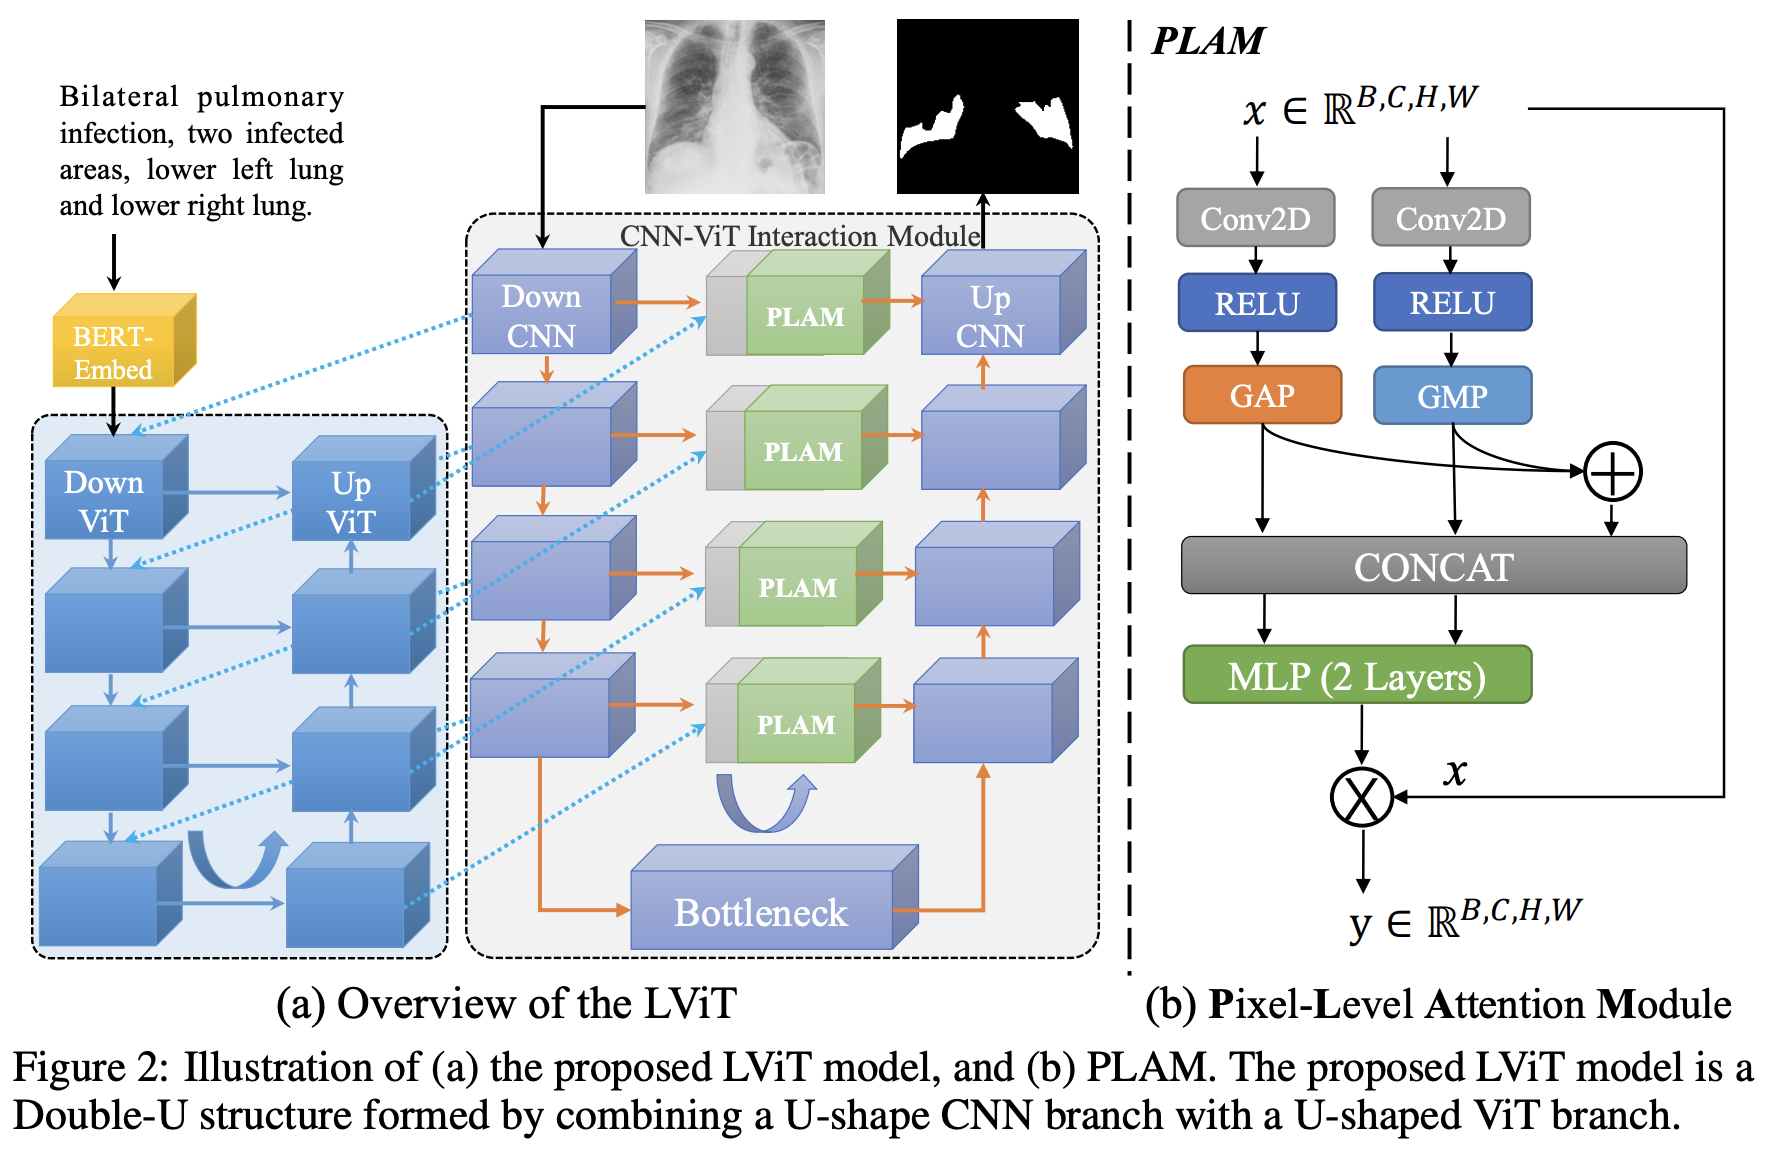
\includegraphics[width=0.92\textwidth]{lvit_original_architecture.png}
  \caption{Kiến trúc tổng quan của LViT.}
  \label{fig:lvit-arch}
\end{figure*}

Hình~\ref{fig:lvit-arch} cho thấy LViT gồm bốn nhóm thành phần chính. Thứ nhất là nhánh CNN dạng U-Net, có nhiệm vụ giữ cấu trúc không gian, biên và chi tiết cục bộ của ảnh. Thứ hai là nhánh Vision Transformer đa mức, chuyển bản đồ đặc trưng thành token để học quan hệ xa giữa các vùng ảnh. Thứ ba là nhánh văn bản, mã hóa văn bản chú thích rồi chiếu biểu diễn văn bản về các mức kênh phù hợp để đưa vào token ảnh. Thứ tư là PLAM và bộ giải mã, giúp nhấn mạnh lại thông tin mức điểm ảnh khi khôi phục mặt nạ.

Có thể đọc LViT theo hai lớp. Lớp hệ thống đã được mô tả ở Hình~\ref{fig:lvit-system-overview}: ảnh, văn bản và mặt nạ nếu có đi vào các công đoạn mã hóa, hợp nhất, học ngữ cảnh, kiểm soát pseudo-label và giải mã phân đoạn. Lớp kiến trúc ở Hình~\ref{fig:lvit-arch} cụ thể hóa các công đoạn đó bằng Double-U CNN--Transformer. CNN dựa trên giả định cục bộ của điểm ảnh nên phù hợp để giữ biên và texture; self-attention trong Transformer học quan hệ xa nên giúp mô hình hiểu bối cảnh toàn ảnh; văn bản branch bổ sung ngữ nghĩa; còn pseudo-label chỉ là nhãn tạm, phải được kiểm soát trong học bán giám sát.

Từ mục 3.2 trở đi, báo cáo mới đi vào từng khối theo trình tự chi tiết hơn: luồng học/kiểm thử, Double-U và Transformer đa mức, biểu diễn văn bản và hợp nhất ảnh--văn bản, PLAM, EPI/LV loss, cuối cùng là loss và metric. Cách tách này giúp 3.1 giữ đúng vai trò tổng quan, còn các mục sau chịu trách nhiệm giải thích nguyên lý, phương pháp và giải thuật của từng thành phần.

\section{Luồng xử lý trong giai đoạn học và kiểm thử}

Mục 3.1 đã mô tả LViT ở mức kiến trúc tổng quan. Mục này chuyển sang luồng hoạt động: cùng một mô hình được dùng như thế nào trong giai đoạn học có nhãn, học bán giám sát và kiểm thử. Đây là phần quan trọng vì một kiến trúc chỉ là ``bản vẽ tĩnh''; để hiểu phương pháp, cần biết dữ liệu đi qua hệ thống ra sao, đầu ra nào được so với ground truth, đầu ra nào chỉ là pseudo-label, và lúc nào mô hình được cập nhật.

\subsection*{Nguyên lý}

Nguyên lý của luồng học/kiểm thử trong LViT là tách rõ ba loại tín hiệu. Tín hiệu thứ nhất là đầu vào luôn có: ảnh \(x\) và văn bản chú thích \(t\). Tín hiệu thứ hai là ground truth \(y\), chỉ tồn tại ở tập có nhãn và được dùng như chuẩn xác thực trong huấn luyện/đánh giá. Tín hiệu thứ ba là pseudo-label \(\tilde{y}\), chỉ là nhãn tạm do mô hình sinh ra cho dữ liệu chưa nhãn. Ba tín hiệu này không được dùng lẫn lộn: ground truth là nhãn chuyên gia, pseudo-label là dự đoán được kiểm soát, còn văn bản là ngữ nghĩa bổ trợ chứ không thay thế mask.

Về bản chất, giai đoạn học là quá trình tìm tham số \(\theta\) sao cho ánh xạ \(f_\theta(x,t)=\hat{y}\) ngày càng gần mặt nạ đúng. Với mẫu có nhãn, ``đúng'' được định nghĩa bằng ground truth \(y\). Với mẫu chưa nhãn, ``đúng tạm thời'' được xấp xỉ bằng pseudo-label đã làm mượt và được ràng buộc thêm bằng văn bản. Giai đoạn kiểm thử thì khác: mô hình không học nữa, không cập nhật tham số nữa, mà chỉ dùng \(x,t\) để sinh \(\hat{y}\). Ground truth của test, nếu có, chỉ dùng để tính Dice và IoU.

\subsection*{Phương pháp}

Trong giai đoạn học có giám sát, mỗi mẫu gồm bộ ba \((x,t,y)\). Ảnh được resize và chuẩn hóa; mặt nạ được đưa về cùng kích thước với ảnh và thường được nhị phân hóa cho bài toán foreground/background; văn bản được chuyển thành embedding. Mô hình sinh mặt nạ xác suất \(\hat{y}\). Sau đó, supervised loss so sánh \(\hat{y}\) với \(y\), ví dụ bằng BCE và Dice loss. Gradient từ loss này cập nhật các tham số của bộ mã hóa ảnh, nhánh Transformer, nhánh văn bản, fusion và bộ giải mã.

Trong giai đoạn học bán giám sát, mẫu chỉ có \((x,t)\), không có mặt nạ \(y\). LViT vẫn forward ảnh và văn bản để sinh \(\hat{y}\), nhưng không thể so trực tiếp với ground truth. Thay vào đó, dự đoán qua các epoch được dùng để tạo pseudo-label. EPI làm mượt pseudo-label theo thời gian để tránh học theo dự đoán nhiễu ở một epoch đơn lẻ. LV loss đưa văn bản vào vai trò kiểm soát ngữ nghĩa cho nhánh chưa nhãn. Vì vậy, dữ liệu chưa nhãn vẫn đóng góp vào quá trình học, nhưng không được đối xử như dữ liệu có ground truth thật.

Trong giai đoạn kiểm thử, hệ thống nhận \((x,t)\), đưa qua cùng forward pass của LViT và sinh \(\hat{y}\). Mặt nạ xác suất này được ngưỡng hóa thành mặt nạ nhị phân. Nếu tập test có ground truth, \(y\) chỉ xuất hiện sau khi dự đoán đã hoàn tất để tính độ đo. Điều này cần nhấn mạnh để tránh hiểu nhầm rằng ground truth được đưa vào mô hình trong lúc kiểm thử.

\subsection*{Giải thuật}

Luồng học và kiểm thử có thể mô tả bằng ba pseudo code sau.

\begin{algorithm}[H]
\caption{Một bước học có giám sát với mẫu có nhãn}
\label{alg:lvit-supervised-step}
\begin{algorithmic}[1]
\Require Mẫu có nhãn \((x,t,y)\), tham số LViT \(\theta\), bộ tối ưu \(\mathrm{Opt}\)
\Ensure Tham số cập nhật \(\theta\), loss có giám sát \(\mathcal{L}_{sup}\)
\State \(\mathrm{SetTrainMode}(\theta)\) \Comment{Bật chế độ học để BatchNorm/Dropout hoạt động đúng trong huấn luyện.}
\State \(x_p \gets \mathrm{PreprocessImage}(x)\) \Comment{Resize, chuẩn hóa cường độ và đưa ảnh về tensor cùng kích thước đầu vào.}
\State \(y_p \gets \mathrm{PreprocessMask}(y)\) \Comment{Đưa mặt nạ thật về cùng kích thước với ảnh; với bài toán nhị phân, mask là foreground/background.}
\State \(e_t \gets \mathrm{EncodeText}(t)\) \Comment{Token hóa văn bản và biến thành embedding; đây là tín hiệu ngữ nghĩa bổ trợ.}
\State \(\mathrm{Opt.zero\_grad}()\) \Comment{Xóa gradient cũ để bước cập nhật hiện tại không bị cộng dồn sai.}
\State \(\{F_x^l\}_{l=1}^{4} \gets \mathrm{ImageEncoder}(x_p;\theta)\) \Comment{CNN trích xuất bản đồ đặc trưng đa mức, giữ cấu trúc không gian và chi tiết cục bộ.}
\State \(\{Z_{mix}^l\}_{l=1}^{4} \gets \mathrm{LVFusion}(\{F_x^l\},e_t;\theta)\) \Comment{Đưa embedding văn bản vào token ảnh ở các mức phù hợp.}
\State \(H \gets \mathrm{HybridCNNTransformer}(\{Z_{mix}^l\};\theta)\) \Comment{Học đồng thời thông tin cục bộ của CNN và quan hệ xa của Transformer.}
\State \(\hat{y} \gets \mathrm{bộ giải mã}(H;\theta)\) \Comment{Khôi phục không gian ảnh và sinh mặt nạ xác suất theo từng điểm ảnh.}
\State \(\mathcal{L}_{BCE} \gets \mathrm{BCELoss}(\hat{y},y_p)\) \Comment{Phạt sai khác xác suất điểm ảnh-wise giữa dự đoán và ground truth.}
\State \(\mathcal{L}_{Dice} \gets \mathrm{DiceLoss}(\hat{y},y_p)\) \Comment{Tối ưu trực tiếp mức chồng lấn vùng, phù hợp khi foreground nhỏ.}
\State \(\mathcal{L}_{sup} \gets \mathcal{L}_{BCE}+\mathcal{L}_{Dice}\) \Comment{Loss có giám sát dùng mặt nạ thật làm đầu ra xác thực.}
\State \(\mathcal{L}_{sup}.\mathrm{backward}()\) \Comment{Lan truyền gradient qua bộ giải mã, Transformer, fusion, văn bản branch và CNN bộ mã hóa.}
\State \(\mathrm{Opt.step}()\) \Comment{Cập nhật tham số \(\theta\) theo gradient của loss có giám sát.}
\State \Return \(\theta,\mathcal{L}_{sup}\) \Comment{Trả về mô hình sau cập nhật và giá trị loss để theo dõi quá trình học.}
\end{algorithmic}
\end{algorithm}

\begin{algorithm}[H]
\caption{Một bước học bán giám sát với mẫu chưa nhãn}
\label{alg:lvit-semisup-step}
\begin{algorithmic}[1]
\Require Mẫu chưa nhãn \((x,t)\), tham số \(\theta\) ở epoch \(k\), pseudo-label cũ \(P_{prev}\), hệ số EPI \(\alpha\), trọng số LV \(\gamma\), bộ tối ưu \(\mathrm{Opt}\)
\Ensure Tham số cập nhật \(\theta\), pseudo-label mới \(P_{curr}\), loss bán giám sát \(\mathcal{L}_{unsup}\)
\State \(\mathrm{SetTrainMode}(\theta)\) \Comment{Vẫn huấn luyện mô hình, nhưng mẫu hiện tại không có mặt nạ thật.}
\State \(x_p \gets \mathrm{PreprocessImage}(x)\) \Comment{Chuẩn hóa ảnh giống nhánh có nhãn để phân bố đầu vào nhất quán.}
\State \(e_t \gets \mathrm{EncodeText}(t)\) \Comment{Văn bản vẫn được dùng vì mẫu chưa nhãn vẫn có văn bản chú thích.}
\State \(\mathrm{Opt.zero\_grad}()\) \Comment{Bắt đầu một bước cập nhật mới cho nhánh chưa nhãn.}
\State \(\hat{y}^{(k)} \gets \mathrm{LViTForward}(x_p,e_t;\theta)\) \Comment{Sinh mặt nạ xác suất hiện tại; đây chưa phải ground truth.}
\State \(\hat{y}_{stop}^{(k)} \gets \mathrm{StopGradient}(\hat{y}^{(k)})\) \Comment{Tách dự đoán dùng làm pseudo-label khỏi đồ thị gradient để tránh tự kéo mục tiêu.}
\If{\(P_{prev}\) chưa tồn tại}
  \State \(P_{curr} \gets \hat{y}_{stop}^{(k)}\) \Comment{Ở lần đầu, pseudo-label tạm thời chính là dự đoán hiện tại.}
\Else
  \State \(P_{curr} \gets \alpha P_{prev} + (1-\alpha)\hat{y}_{stop}^{(k)}\) \Comment{EPI làm mượt pseudo-label qua thời gian, giảm nhiễu của một epoch đơn lẻ.}
\EndIf
\State \(P_{bin} \gets \mathrm{OptionalThreshold}(P_{curr})\) \Comment{Có thể chuyển pseudo-label thành mục tiêu rõ hơn tùy cấu hình; vẫn không phải nhãn chuyên gia.}
\State \(\mathcal{L}_{pseudo} \gets \mathrm{BCEDiceLoss}(\hat{y}^{(k)},P_{bin})\) \Comment{Buộc dự đoán hiện tại nhất quán với pseudo-label đã làm mượt.}
\State \(\mathcal{L}_{LV} \gets \mathrm{LVLoss}(e_t,\hat{y}^{(k)},P_{curr})\) \Comment{Dùng tín hiệu văn bản để kiểm soát ngữ nghĩa của nhánh chưa nhãn.}
\State \(\mathcal{L}_{unsup} \gets \mathcal{L}_{pseudo}+\gamma\mathcal{L}_{LV}\) \Comment{Tổng loss chưa giám sát gồm ràng buộc pseudo-mask và ràng buộc ảnh--văn bản.}
\State \(\mathcal{L}_{unsup}.\mathrm{backward}()\) \Comment{Gradient chỉ cập nhật mô hình, không cập nhật pseudo-label đã stop-gradient.}
\State \(\mathrm{Opt.step}()\) \Comment{Cập nhật \(\theta\) bằng tín hiệu từ mẫu chưa nhãn đã được kiểm soát.}
\State \Return \(\theta,P_{curr},\mathcal{L}_{unsup}\) \Comment{Lưu \(P_{curr}\) để dùng làm pseudo-label cũ ở epoch hoặc vòng lặp sau.}
\end{algorithmic}
\end{algorithm}

\begin{algorithm}[H]
\caption{Suy luận và đánh giá trên tập kiểm thử}
\label{alg:lvit-inference}
\begin{algorithmic}[1]
\Require Mẫu kiểm thử \((x,t)\), tham số đã huấn luyện \(\theta\), mặt nạ \(y\) nếu có, ngưỡng \(\tau\)
\Ensure Mặt nạ nhị phân \(\hat{y}_{bin}\), độ đo Dice/IoU nếu có \(y\)
\State \(\mathrm{SetEvalMode}(\theta)\) \Comment{Tắt hành vi ngẫu nhiên của Dropout và dùng thống kê cố định của BatchNorm.}
\State \(\mathrm{DisableGradient}()\) \Comment{Không tính gradient vì suy luận không cập nhật mô hình.}
\State \(x_p \gets \mathrm{PreprocessImage}(x)\) \Comment{Áp dụng đúng chuẩn hóa như lúc học để tránh lệch phân bố.}
\State \(e_t \gets \mathrm{EncodeText}(t)\) \Comment{Mã hóa văn bản đi kèm; văn bản là đầu vào của mô hình, không phải ground truth.}
\State \(\{F_x^l\}_{l=1}^{4} \gets \mathrm{ImageEncoder}(x_p;\theta)\) \Comment{Trích xuất đặc trưng ảnh đa mức.}
\State \(\{Z_{mix}^l\}_{l=1}^{4} \gets \mathrm{LVFusion}(\{F_x^l\},e_t;\theta)\) \Comment{Hợp nhất thông tin ảnh và văn bản trước các khối Transformer.}
\State \(H \gets \mathrm{HybridCNNTransformer}(\{Z_{mix}^l\};\theta)\) \Comment{Tạo biểu diễn đã học cả chi tiết cục bộ và ngữ cảnh xa.}
\State \(\hat{y} \gets \mathrm{bộ giải mã}(H;\theta)\) \Comment{Sinh mặt nạ xác suất, mỗi điểm ảnh có giá trị thuộc \([0,1]\).}
\State \(\hat{y}_{bin} \gets \mathrm{Threshold}(\hat{y},\tau)\) \Comment{Ngưỡng hóa xác suất để tạo mặt nạ foreground/background cuối cùng.}
\If{\(y\) tồn tại}
  \State \(y_p \gets \mathrm{PreprocessMask}(y)\) \Comment{Ground truth chỉ dùng sau khi dự đoán xong để đánh giá, không đưa vào mô hình.}
  \State \(\mathrm{metrics} \gets \mathrm{ComputeDiceIoU}(\hat{y}_{bin},y_p)\) \Comment{Tính Dice/IoU dựa trên mặt nạ dự đoán và mặt nạ thật.}
\Else
  \State \(\mathrm{metrics} \gets \varnothing\) \Comment{Nếu không có ground truth, chỉ xuất mặt nạ dự đoán để quan sát hoặc hậu xử lý.}
\EndIf
\State \Return \(\hat{y}_{bin},\mathrm{metrics}\) \Comment{Không có backpropagation và không có optimizer step trong giai đoạn suy luận.}
\end{algorithmic}
\end{algorithm}

\begin{figure}[H]
    \centering
    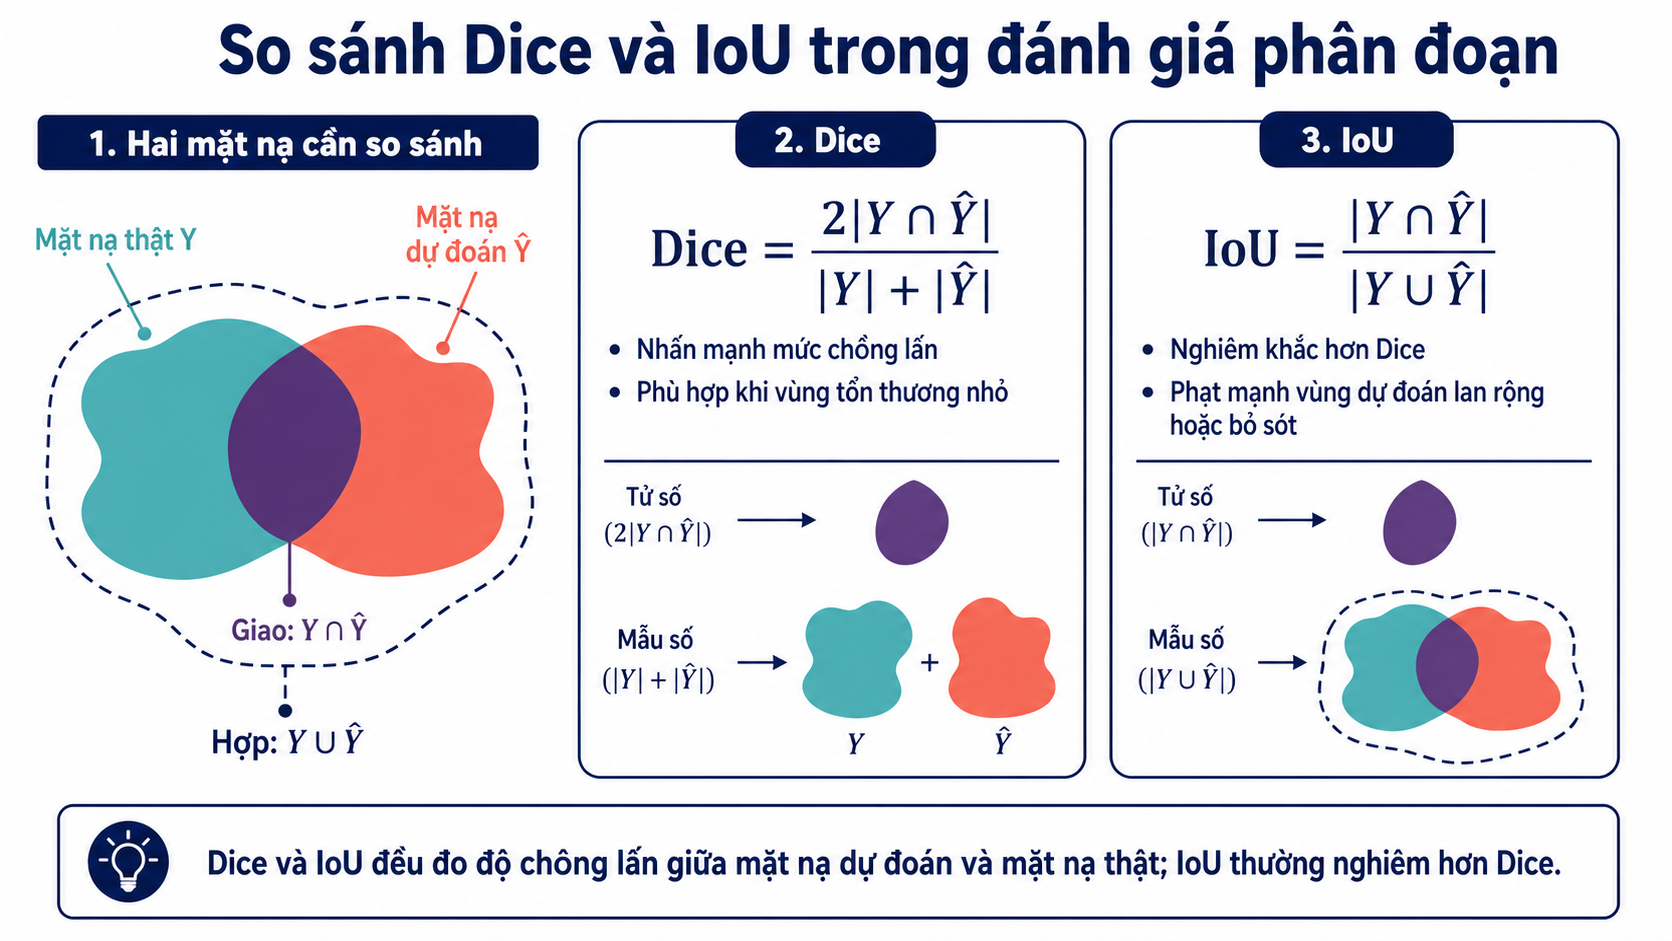
\includegraphics[width=0.92\textwidth]{figures/dice_iou_comparison_generated.png}
    \caption{Diễn giải Dice và IoU trong đánh giá phân đoạn. Cả hai độ đo đều dựa trên phần giao giữa mặt nạ dự đoán \(\hat{Y}\) và mặt nạ thật \(Y\), nhưng Dice chuẩn hóa theo tổng diện tích hai mặt nạ, còn IoU chuẩn hóa theo phần hợp nên thường nghiêm khắc hơn khi dự đoán lan rộng hoặc bỏ sót vùng tổn thương.}
    \label{fig:ch3-dice-iou-comparison}
\end{figure}

Hình~\ref{fig:ch3-dice-iou-comparison} làm rõ vì sao trong pseudo code đánh giá cần tính cả Dice và IoU. Dice nhấn mạnh mức chồng lấn và thường dễ đọc khi vùng tổn thương nhỏ, vì phần giao được nhân đôi trong tử số. IoU thì so phần giao với toàn bộ phần hợp, nên nếu mô hình dự đoán quá rộng ra nền phổi hoặc bỏ sót nhiều vùng tổn thương, điểm IoU giảm mạnh hơn. Vì vậy, trong LViT, loss có thể dùng BCE/Dice để tối ưu quá trình học, nhưng phần đánh giá vẫn cần báo cáo cả Dice và IoU để nhìn được cả độ phủ và mức false positive của mặt nạ cuối.

\begin{figure}[H]
    \centering
    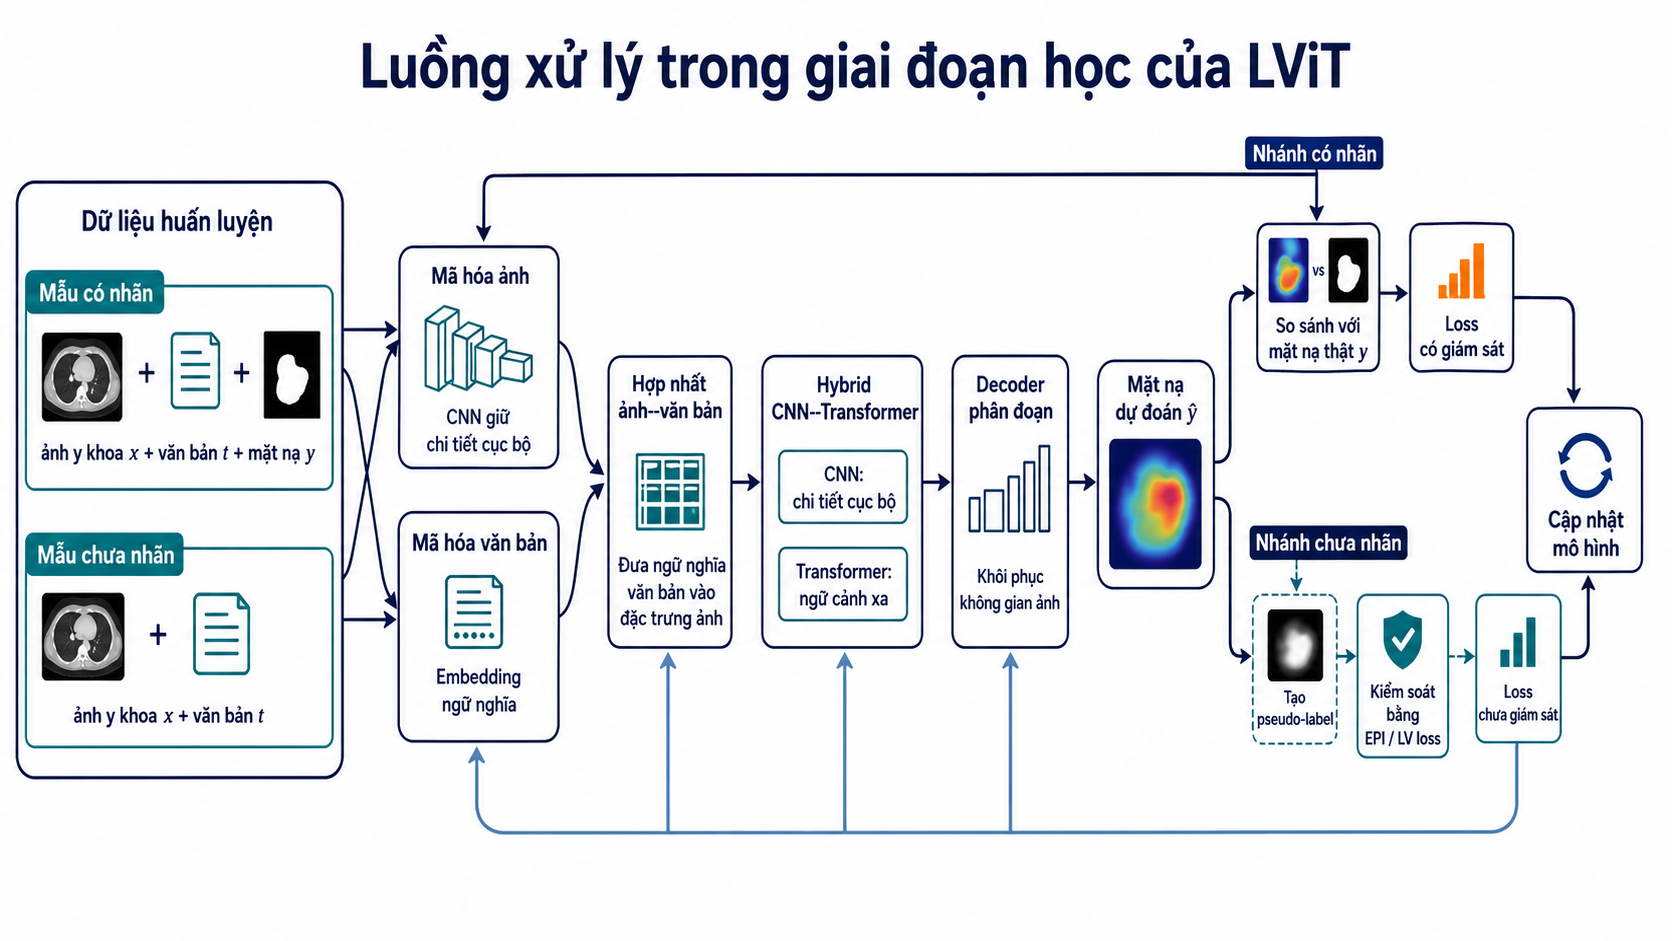
\includegraphics[width=\textwidth]{figures/lvit_training_flow_generated.png}
    \caption{Luồng xử lý trong giai đoạn học của LViT ở mức tổng quan. Mẫu có nhãn dùng mặt nạ thật để tạo loss có giám sát; mẫu chưa nhãn dùng pseudo-label và cơ chế EPI/LV loss để tạo loss chưa giám sát. Sơ đồ giản lược các tầng chi tiết để nhấn mạnh đường đi của dữ liệu và tín hiệu cập nhật mô hình.}
    \label{fig:lvit-training-flow-generated}
\end{figure}

\begin{figure}[H]
    \centering
    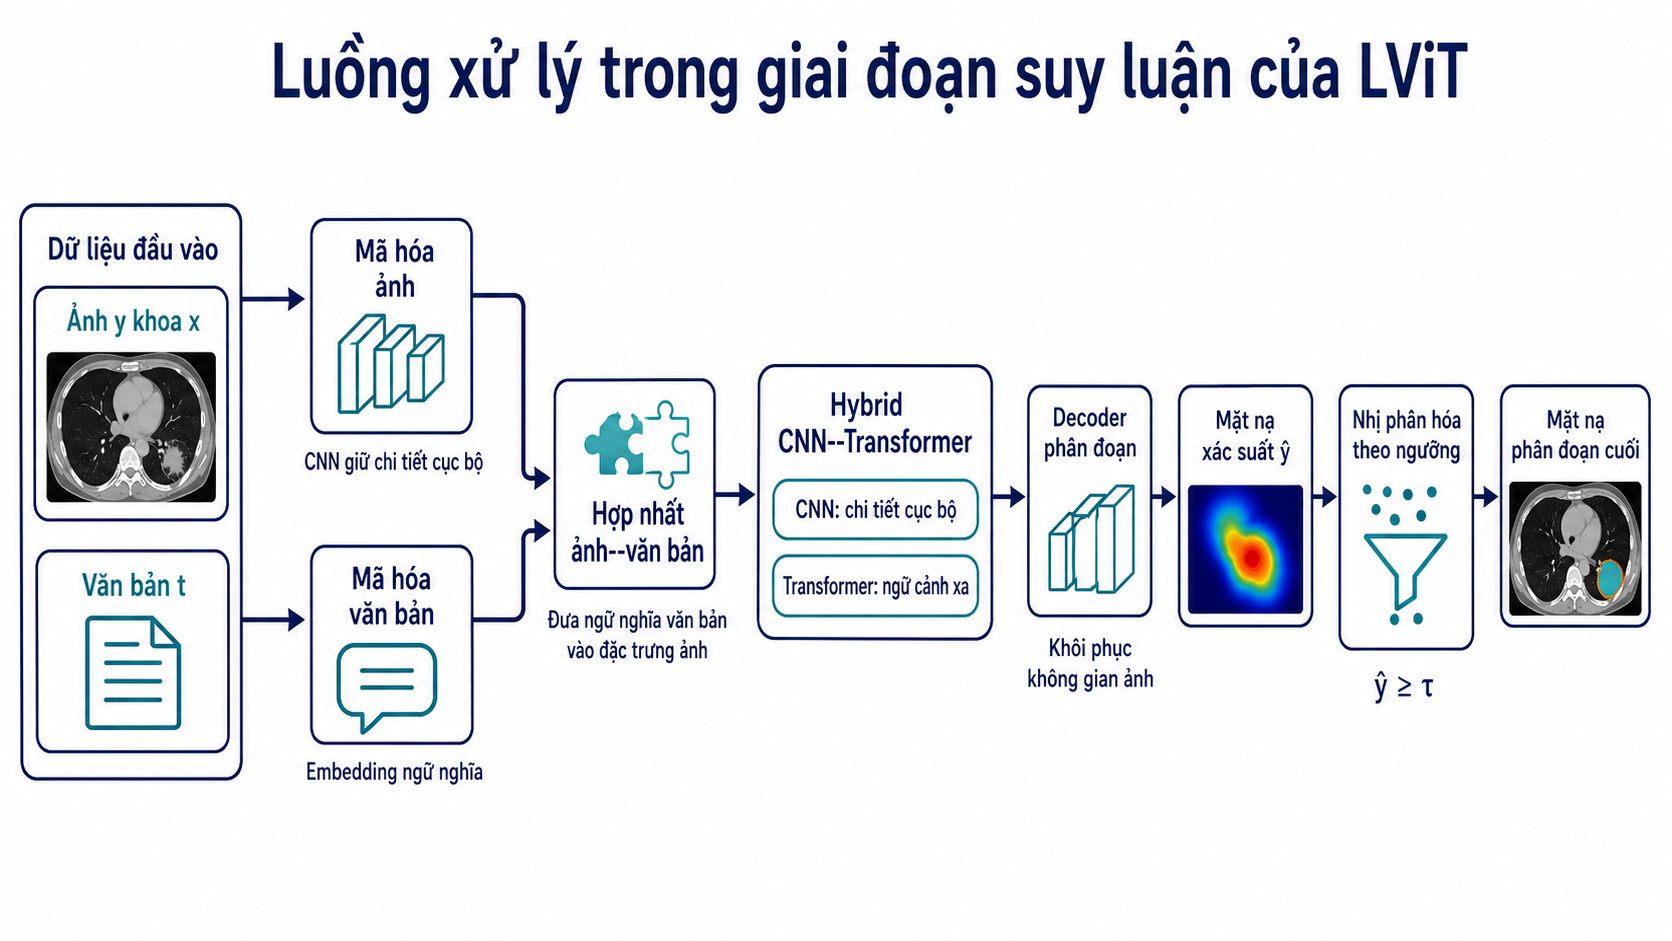
\includegraphics[width=\textwidth]{figures/lvit_inference_flow_generated.png}
    \caption{Luồng xử lý trong giai đoạn suy luận của LViT ở mức tổng quan. Ở giai đoạn này, mô hình chỉ nhận ảnh y khoa và văn bản lâm sàng, sinh mặt nạ xác suất, rồi nhị phân hóa theo ngưỡng để tạo mặt nạ phân đoạn cuối; không có ground truth, loss hay cập nhật trọng số.}
    \label{fig:lvit-inference-flow-generated}
\end{figure}

Có thể hình dung luồng xử lý bằng hai đường song song như Hình~\ref{fig:lvit-training-flow-generated} và Hình~\ref{fig:lvit-inference-flow-generated}. Đường có nhãn đi từ \((x,t,y)\) đến \(\hat{y}\), rồi loss so sánh trực tiếp \(\hat{y}\) với \(y\). Đường chưa nhãn đi từ \((x,t)\) đến \(\hat{y}\), sau đó \(\hat{y}\) được biến thành pseudo-label và được EPI/LV loss kiểm soát trước khi dùng để học. Khi kiểm thử, chỉ còn đường \((x,t)\rightarrow\hat{y}\rightarrow\) mặt nạ nhị phân. Các chi tiết kiến trúc cụ thể có thể đọc từ hình tổng quan LViT ở Hình~\ref{fig:lvit-arch}.

\section{Kiến trúc Double-U và Vision Transformer đa mức}

Mục 3.1 đã nói LViT cần đồng thời giữ chi tiết cục bộ và học ngữ cảnh xa. Mục này đi vào cách LViT hiện thực hóa yêu cầu đó bằng kiến trúc Double-U: một nhánh U-shaped CNN xử lý bản đồ đặc trưng không gian, và một nhánh U-shaped Vision Transformer xử lý token đa mức. Đây là khối trả lời trực tiếp Gap 1 ở Chương 2: nếu chỉ dùng CNN thì thiếu quan hệ xa; nếu chỉ dùng Transformer thì dễ làm yếu cấu trúc cục bộ và tốn dữ liệu. Double-U là cách để hai thiên kiến này bổ sung cho nhau.

\begin{figure}[H]
    \centering
    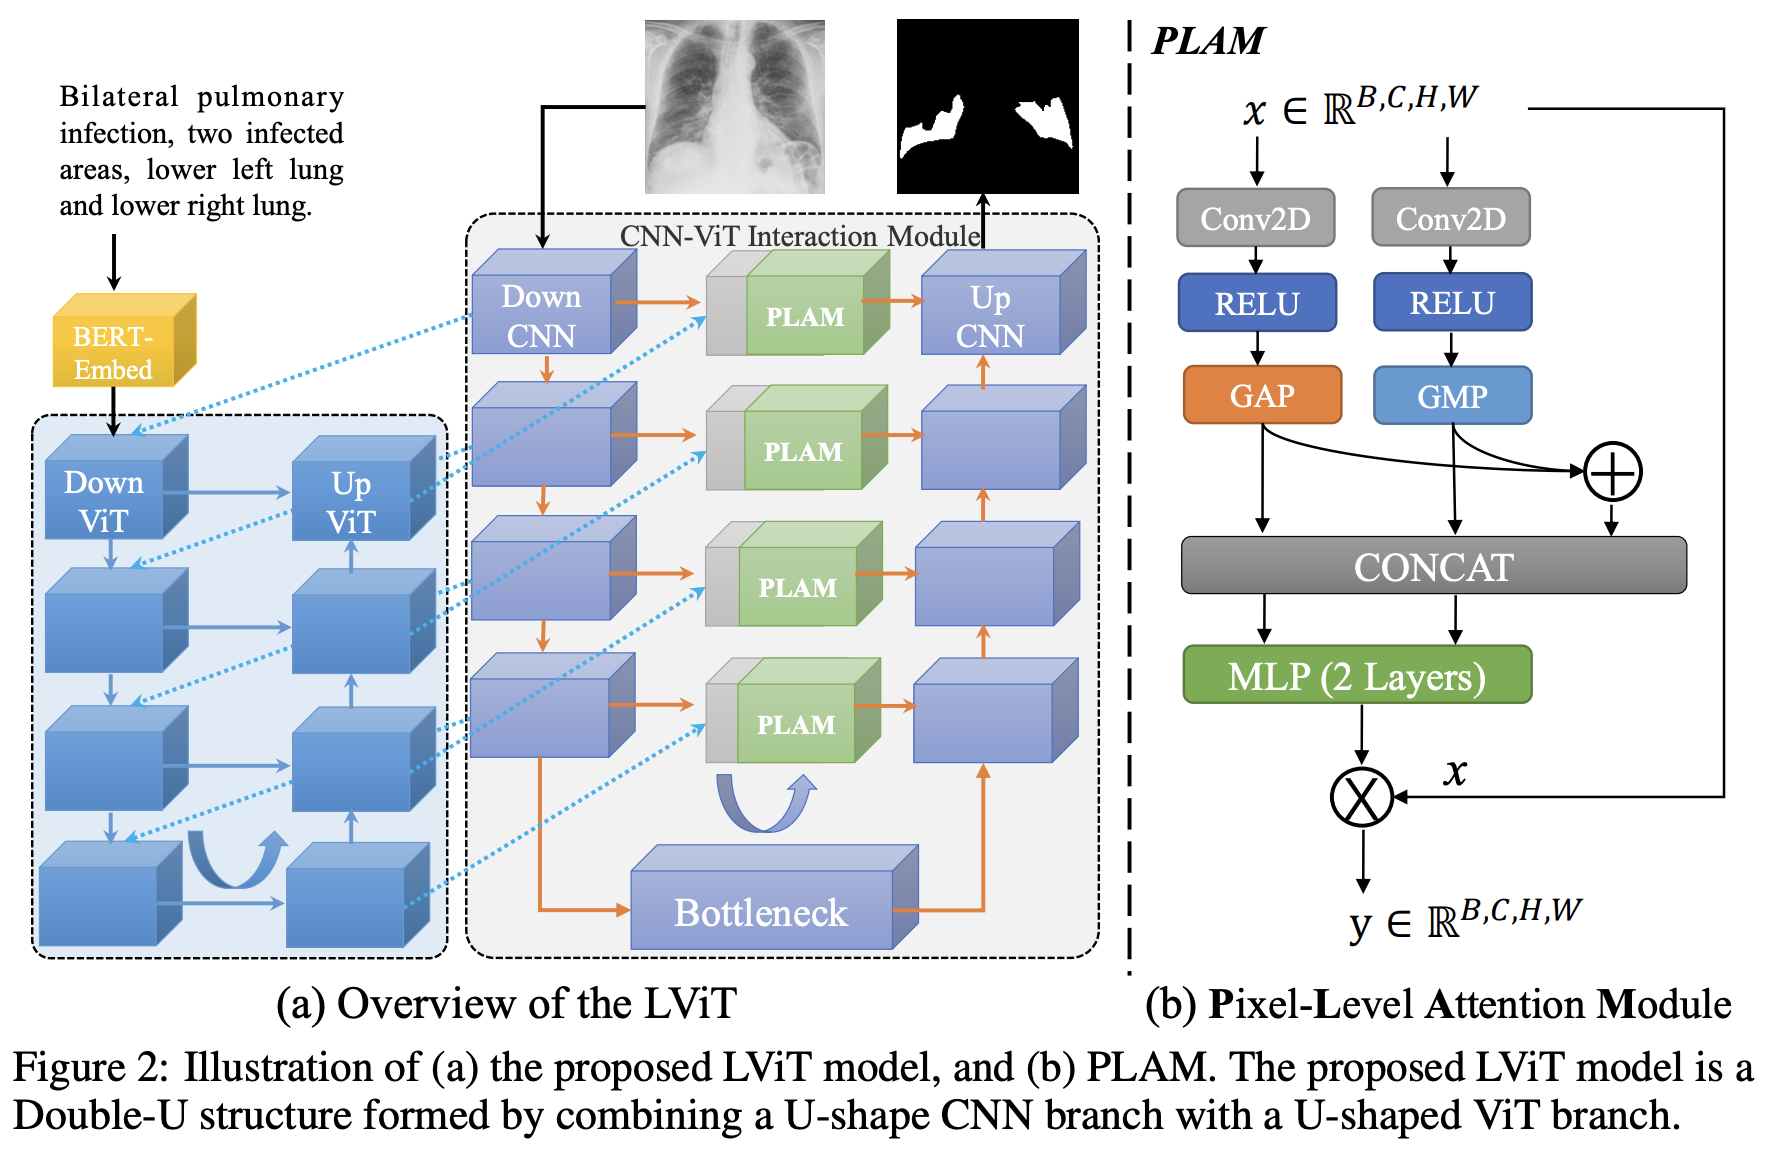
\includegraphics[width=\textwidth]{lvit_original_architecture.png}
    \caption{Kiến trúc Double-U của LViT trong bài báo gốc \cite{li2023lvit}. Phần bên trái thể hiện nhánh U-shaped ViT xử lý token đa mức; phần giữa thể hiện nhánh U-shaped CNN giữ bản đồ đặc trưng không gian và bộ giải mã phân đoạn; các đường nối giữa hai nhánh cho thấy đặc trưng ảnh được chuyển qua lại giữa không gian điểm ảnh và không gian token. Hình này cần được đọc như một mô hình lai: CNN bảo vệ chi tiết cục bộ, còn Transformer học ngữ cảnh xa.}
    \label{fig:lvit-double-u-original}
\end{figure}

\subsection*{Nguyên lý}

Nguyên lý của Double-U là tách hai loại tri thức thị giác nhưng không để chúng rời nhau. CNN học theo lân cận điểm ảnh:
\[
F_x^{l}=I_l(F_x^{l-1}),
\]
trong đó \(F_x^l\) là bản đồ đặc trưng ở mức \(l\), còn \(I_l\) là khối convolution/downsample. Vì convolution dùng kernel cục bộ, nó phù hợp để học biên, texture và cấu trúc nhỏ. Tuy nhiên, convolution phải chồng nhiều lớp mới có trường nhìn rộng, nên việc học quan hệ xa không trực tiếp.

Transformer xử lý bản đồ đặc trưng bằng cách biến từng vùng ảnh thành token. Nếu gọi \(Z^l\in\mathbb{R}^{N_l\times d_l}\) là tập token ở mức \(l\), self-attention học quan hệ giữa các token bằng:
\[
\mathrm{Attention}(Q,K,V)
=\mathrm{softmax}\left(\frac{QK^\top}{\sqrt{d}}\right)V.
\]
Công thức này có nghĩa là mỗi token không chỉ nhìn các token lân cận, mà có thể gán trọng số cho mọi token khác trong cùng bản đồ đặc trưng. Đây là lý do attention phù hợp để học ngữ cảnh xa: một vùng nghi ngờ ở ảnh y khoa có thể được diễn giải dựa trên toàn cơ quan, không chỉ vài điểm ảnh bên cạnh.

Kết luận nguyên lý của Double-U là: CNN giữ bản đồ không gian và chi tiết cục bộ, Transformer học quan hệ xa trên token, còn kết nối giữa hai nhánh giúp thông tin không bị chia thành hai thế giới độc lập.

\subsection*{Phương pháp}

Trong triển khai LViT, nhánh CNN có dạng U-Net: khối đầu tạo đặc trưng ban đầu, các khối downsampling giảm dần độ phân giải và tăng số kênh, sau đó các khối upsampling khôi phục độ phân giải bằng skip connection. Đây là đường giữ cấu trúc ảnh, vì các bản đồ đặc trưng vẫn có dạng \((C,H,W)\).

Song song, LViT đặt các Vision Transformer ở bốn mức đặc trưng. Với ảnh vào kích thước \(224\times224\), các mức đặc trưng có kích thước \(224,112,56,28\), patch size tương ứng \(16,8,4,2\), và embedding dimension \(64,128,256,512\). Điểm đáng chú ý là các lựa chọn này đều tạo số patch \(14\times14=196\) ở mỗi mức. Như vậy, mỗi mức có cùng số token nhưng khác kênh/ngữ nghĩa: mức nông giữ chi tiết hơn, mức sâu chứa ngữ nghĩa mạnh hơn.

\begin{table*}[!t]
  \centering
  \caption{Các mức Vision Transformer trong LViT.}
  \label{tab:lvit-vit-levels}
  \scriptsize
  \renewcommand{\arraystretch}{1.12}
  \setlength{\tabcolsep}{5pt}
  \begin{tabularx}{\textwidth}{@{}l Y Y Y Y@{}}
    \toprule
    Mức & Kích thước đặc trưng & Patch size & Số token & Embedding dim \\
    \midrule
    Level 1 & \(224\times224\) & \(16\times16\) & 196 & 64 \\
    Level 2 & \(112\times112\) & \(8\times8\) & 196 & 128 \\
    Level 3 & \(56\times56\) & \(4\times4\) & 196 & 256 \\
    Level 4 & \(28\times28\) & \(2\times2\) & 196 & 512 \\
    \bottomrule
  \end{tabularx}
\end{table*}
\FloatBarrier

Trong nhánh Transformer, khối embedding biến bản đồ đặc trưng thành token; block Transformer gồm attention, MLP, residual và normalization; khối tái dựng chuyển token trở lại bản đồ đặc trưng khi cần. Ở một số nhánh, token hiện tại còn được ghép hoặc cộng với token skip từ mức trước/sau để tạo luồng U-shaped trong Transformer. Vì vậy, chữ ``Double-U'' không chỉ nghĩa là có U-Net CNN, mà còn có một trục U-shaped ở phía token.

\subsection*{Giải thuật}

Trình tự xử lý của Double-U có thể mô tả bằng pseudo code như sau:

\begin{algorithm}[H]
\caption{Forward của kiến trúc Double-U CNN--ViT}
\label{alg:double-u-forward}
\begin{algorithmic}[1]
\Require Ảnh \(x\), đặc trưng văn bản đã chiếu \(\{E_t^l\}_{l=1}^{4}\), tham số kiến trúc \(\theta\)
\Ensure Mặt nạ xác suất \(\hat{y}\)
\State \(x_1 \gets \mathrm{InitialConv}(x)\) \Comment{Tạo bản đồ đặc trưng nông nhất; mức này còn giữ nhiều biên và texture.}
\State \(y_1 \gets \mathrm{DownViT}_{1}(x_1,\mathrm{skip}=x_1,\mathrm{văn bản}=E_t^1)\) \Comment{Đưa đặc trưng mức 1 thành token và hợp nhất với văn bản cùng chiều.}
\State \(x_2 \gets \mathrm{DownBlock}_{1}(x_1)\) \Comment{Giảm độ phân giải ảnh để tăng trường nhìn và số kênh.}
\State \(y_2 \gets \mathrm{DownViT}_{2}(x_2,\mathrm{skip}=y_1,\mathrm{văn bản}=E_t^2)\) \Comment{Mức 2 nhận thêm token skip từ mức trước để tạo nhánh ViT dạng U.}
\State \(x_3 \gets \mathrm{DownBlock}_{2}(x_2)\) \Comment{đặc trưng sâu hơn chứa ít chi tiết điểm ảnh hơn nhưng giàu ngữ nghĩa hơn.}
\State \(y_3 \gets \mathrm{DownViT}_{3}(x_3,\mathrm{skip}=y_2,\mathrm{văn bản}=E_t^3)\) \Comment{Transformer tiếp tục học quan hệ xa trên token đa mức.}
\State \(x_4 \gets \mathrm{DownBlock}_{3}(x_3)\) \Comment{Mức sâu gần bottleneck, phù hợp để gom bối cảnh toàn ảnh.}
\State \(y_4 \gets \mathrm{DownViT}_{4}(x_4,\mathrm{skip}=y_3,\mathrm{văn bản}=E_t^4)\) \Comment{Mức văn bản sâu nhất được dùng để điều kiện hóa token có ngữ nghĩa cao.}
\State \(x_5 \gets \mathrm{DownBlock}_{4}(x_4)\) \Comment{Bottleneck CNN lưu biểu diễn cô đọng trước khi bộ giải mã phục hồi không gian.}
\State \(y_4 \gets \mathrm{UpViT}_{4}(y_4,\mathrm{skip}=y_4,\mathrm{văn bản}=E_t^4)\) \Comment{Bắt đầu nhánh ViT đi lên, xử lý lại token sâu trước khi tái dựng.}
\State \(y_3 \gets \mathrm{UpViT}_{3}(y_3,\mathrm{skip}=y_4,\mathrm{văn bản}=E_t^3)\) \Comment{Kết hợp token mức 3 với thông tin đã đi qua mức sâu hơn.}
\State \(y_2 \gets \mathrm{UpViT}_{2}(y_2,\mathrm{skip}=y_3,\mathrm{văn bản}=E_t^2)\) \Comment{Dòng token đi lên dần trở lại các mức có độ phân giải cao hơn.}
\State \(y_1 \gets \mathrm{UpViT}_{1}(y_1,\mathrm{skip}=y_2,\mathrm{văn bản}=E_t^1)\) \Comment{Token mức nông nhận cả văn bản và ngữ cảnh từ các mức sâu.}
\State \(x_{4}^{mix} \gets \mathrm{Reconstruct}(y_4)+x_4\) \Comment{Đổi token sâu về bản đồ đặc trưng rồi cộng với đặc trưng CNN cùng mức.}
\State \(x_{3}^{mix} \gets \mathrm{Reconstruct}(y_3)+x_3\) \Comment{Trả ngữ cảnh Transformer về không gian ảnh ở mức 3.}
\State \(x_{2}^{mix} \gets \mathrm{Reconstruct}(y_2)+x_2\) \Comment{Giữ song song cục bộ đặc trưng của CNN và toàn cục context của ViT.}
\State \(x_{1}^{mix} \gets \mathrm{Reconstruct}(y_1)+x_1\) \Comment{Mức nông nhất giúp bộ giải mã khôi phục biên và vùng nhỏ.}
\State \(d_4 \gets \mathrm{UpBlockAttention}(x_5,x_{4}^{mix})\) \Comment{bộ giải mã bắt đầu phục hồi từ bottleneck và skip đặc trưng đã trộn.}
\State \(d_3 \gets \mathrm{UpBlockAttention}(d_4,x_{3}^{mix})\) \Comment{Tăng độ phân giải, đồng thời bổ sung chi tiết ở mức trung gian.}
\State \(d_2 \gets \mathrm{UpBlockAttention}(d_3,x_{2}^{mix})\) \Comment{Tiếp tục khôi phục cấu trúc không gian của vùng cần phân đoạn.}
\State \(d_1 \gets \mathrm{UpBlockAttention}(d_2,x_{1}^{mix})\) \Comment{Mức cuối ưu tiên biên, texture và tín hiệu mức điểm ảnh.}
\State \(\hat{y} \gets \mathrm{OutputConv}(d_1)\) \Comment{Chuyển đặc trưng bộ giải mã thành bản đồ xác suất foreground/background.}
\State \Return \(\hat{y}\) \Comment{Đầu ra vẫn là xác suất; loss/threshold sẽ được xử lý ở các bước sau.}
\end{algorithmic}
\end{algorithm}



Trong Hình~\ref{fig:lvit-arch}, trục CNN có thể đọc như đường giữ hình học ảnh: xuống để lấy ngữ nghĩa, lên để phục hồi mặt nạ. Các khối Transformer nằm song song có thể đọc như đường học ngữ cảnh: bản đồ đặc trưng được tách thành patch/token, qua attention, rồi trả lại cho không gian ảnh. Cách đọc đúng là không xem Transformer thay thế CNN, mà xem Transformer như một nhánh bổ sung ngữ cảnh xa cho bản đồ đặc trưng CNN. Vì vậy, nếu CNN là phần trả lời ``vùng biên và texture nằm ở đâu'', thì Vision Transformer là phần trả lời ``vùng này liên hệ với toàn ảnh như thế nào''.

\section{Biểu diễn văn bản và hợp nhất ảnh--văn bản}

Nếu mục trước giải thích cách LViT học ảnh, mục này giải thích cách LViT đưa văn bản vào ảnh. Đây là phần dễ bị hiểu sai nhất: văn bản chú thích không phải nhãn phân loại thay cho mask, cũng không phải câu lệnh để mô hình tô vùng tùy ý. Trong LViT, văn bản là tín hiệu ngữ nghĩa bổ trợ, được biến thành vector rồi đưa vào biểu diễn ảnh để giúp mô hình diễn giải vùng mơ hồ tốt hơn.

\begin{figure}[H]
    \centering
    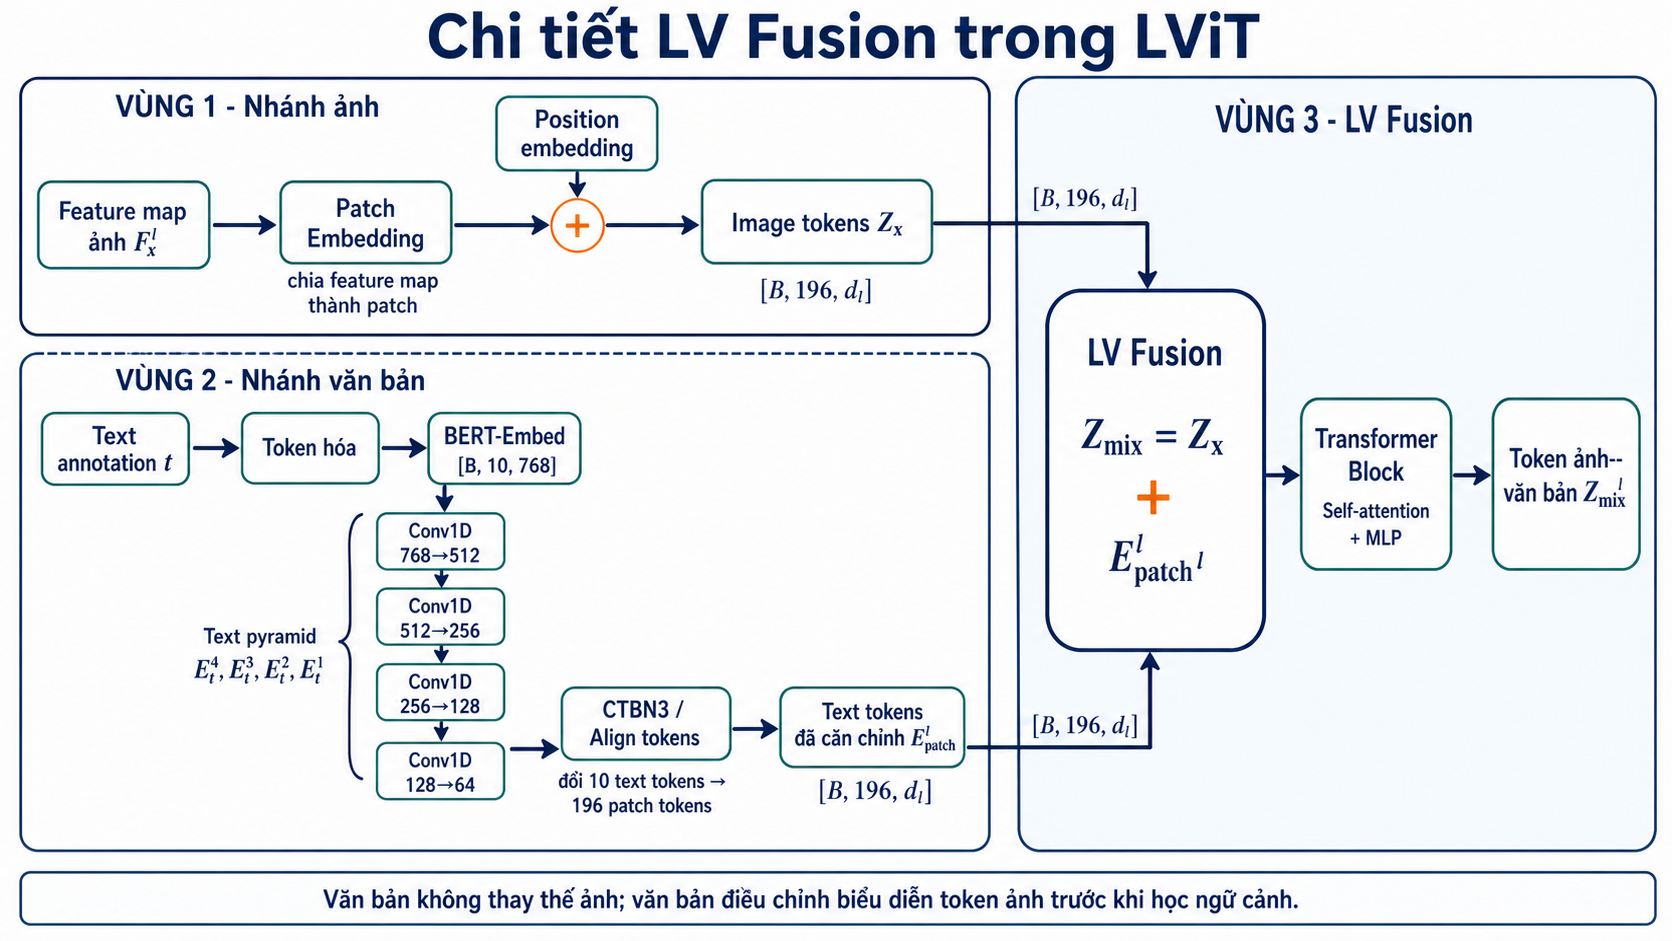
\includegraphics[width=\textwidth]{figures/lvit_lv_fusion_generated.png}
    \caption{Chi tiết LV Fusion trong LViT. Nhánh ảnh chuyển bản đồ đặc trưng thành image tokens và cộng position embedding; nhánh văn bản token hóa văn bản chú thích, mã hóa bằng BERT-Embed, tạo văn bản pyramid qua các lớp Conv1D, rồi căn chỉnh số token từ văn bản tokens sang patch tokens. Khi image tokens và văn bản tokens đã cùng dạng \([B,196,d_l]\), LV Fusion cộng hai biểu diễn để tạo token ảnh--văn bản trước Transformer block.}
    \label{fig:lvit-lv-fusion-generated}
\end{figure}

\subsection*{Nguyên lý}

Văn bản \(t=(w_1,\ldots,w_L)\) ban đầu là chuỗi từ, không thể cộng trực tiếp với ảnh. Do đó cần một bộ mã hóa:
\[
E_t = T(t)\in\mathbb{R}^{L\times d_t},
\]
trong đó \(E_t\) là embedding văn bản. Nếu ảnh ở mức \(l\) có token/đặc trưng chiều \(d_l\), thì văn bản phải được chiếu về cùng không gian:
\[
E_t^l = P_l(E_t), \qquad F_{xt}^l=\Phi_l(F_x^l,E_t^l).
\]
Ý nghĩa của công thức là văn bản không tồn tại như thông tin phụ nằm ngoài mô hình, mà được biến thành đặc trưng cùng ngôn ngữ với ảnh. Phép \(\Phi_l\) có thể là cộng, ghép, attention hoặc một phép biến đổi học được. Điểm quan trọng là sau fusion, đặc trưng \(F_{xt}^l\) vẫn phải sinh mask trên ảnh, nên văn bản chỉ định hướng biểu diễn chứ không thay bằng chứng thị giác.

\subsection*{Phương pháp}

Paper LViT dùng BERT-Embed để thu embedding văn bản 768 chiều \cite{li2023lvit}. Sau bước token hóa, văn bản được đưa qua lớp embedding BERT, rồi qua các lớp chiếu một chiều để giảm dần chiều biểu diễn:
\[
768 \rightarrow 512 \rightarrow 256 \rightarrow 128 \rightarrow 64.
\]
Các mức này tương ứng với bốn mức đặc trưng của LViT, giúp văn bản có thể được đưa vào nhánh Transformer theo đúng kích thước kênh.

Ở nhánh có embedding dimension 64, thao tác hợp nhất có thể diễn giải bằng phép cộng token ảnh--văn bản:
\[
Z = Z_x + \mathrm{CTBN3}(E_t^1),
\]
Ở đây, khối chuyển đổi văn bản đưa biểu diễn văn bản sang cùng số token với token ảnh, rồi cộng vào token ảnh trước khi qua Transformer block. Các mức văn bản khác vẫn được tính và truyền vào các Vision Transformer tương ứng; đồng thời nhánh token đa mức tiếp tục truyền thông tin qua các skip/cộng/ghép trong Transformer. Vì vậy, khi mô tả LViT, cách nói thận trọng là: văn bản được mã hóa, chiếu theo nhiều mức và được dùng trong luồng Vision Transformer; phép cộng trực tiếp văn bản--image token là một cách hiện thực cụ thể của ý tưởng này.

\subsection*{Giải thuật}

Quy trình biểu diễn và hợp nhất văn bản có thể viết bằng pseudo code như sau:

\begin{algorithm}[H]
\caption{Mã hóa văn bản và hợp nhất ảnh--văn bản}
\label{alg:văn bản-fusion}
\begin{algorithmic}[1]
\Require văn bản chú thích \(t\), token ảnh \(\{Z_{img}^{l}\}_{l=1}^{4}\)
\Ensure Token ảnh--văn bản \(\{Z_{mix}^{l}\}_{l=1}^{4}\), đặc trưng văn bản \(\{E_t^l\}_{l=1}^{4}\)
\State \(\mathrm{token\_ids} \gets \mathrm{Tokenize}(t)\) \Comment{Biến câu mô tả lâm sàng thành chuỗi chỉ số từ/token.}
\State \(E_{768} \gets \mathrm{BERTEmbedding}(\mathrm{token\_ids})\) \Comment{Thu embedding ngữ nghĩa 768 chiều cho từng token văn bản.}
\State \(E_t^4 \gets \mathrm{Conv1D}_{768\rightarrow512}(E_{768})\) \Comment{Chiếu văn bản về chiều 512 để khớp mức đặc trưng sâu nhất.}
\State \(E_t^3 \gets \mathrm{Conv1D}_{512\rightarrow256}(E_t^4)\) \Comment{Tạo văn bản đặc trưng cho mức ViT có embedding dimension 256.}
\State \(E_t^2 \gets \mathrm{Conv1D}_{256\rightarrow128}(E_t^3)\) \Comment{Tạo văn bản đặc trưng cho mức trung gian 128 kênh.}
\State \(E_t^1 \gets \mathrm{Conv1D}_{128\rightarrow64}(E_t^2)\) \Comment{Tạo văn bản đặc trưng cho mức nông nhất, nơi token ảnh có 64 chiều.}
\For{\(l \gets 1\) \textbf{to} \(4\)}
  \State \(N_l \gets \mathrm{NumTokens}(Z_{img}^{l})\) \Comment{Lấy số patch token ảnh ở mức \(l\), thường là \(14\times14=196\).}
  \State \(E_{patch}^{l} \gets \mathrm{AlignTextTokens}(E_t^l,N_l)\) \Comment{Đổi văn bản tokens sang cùng số token với ảnh để hai tensor có thể tương tác.}
  \If{\(l\) là mức dùng phép cộng văn bản--image token}
    \State \(Z_{mix}^{l} \gets Z_{img}^{l}+E_{patch}^{l}\) \Comment{Cộng trực tiếp văn bản token đã căn chỉnh vào image token cùng chiều.}
  \Else
    \State \(Z_{mix}^{l} \gets \mathrm{PassTextCondition}(Z_{img}^{l},E_{patch}^{l})\) \Comment{Truyền văn bản như điều kiện cho khối ViT ở mức tương ứng.}
  \EndIf
  \State \(Z_{mix}^{l} \gets \mathrm{TransformerBlock}(Z_{mix}^{l})\) \Comment{Self-attention học quan hệ xa trên token đã mang thông tin ảnh--văn bản.}
\EndFor
\State \Return \(\{Z_{mix}^{l}\}_{l=1}^{4}, \{E_t^l\}_{l=1}^{4}\) \Comment{Trả về token đã fusion và văn bản pyramid để các mức sau tiếp tục sử dụng.}
\end{algorithmic}
\end{algorithm}



Có thể hình dung văn bản branch như một đường ``phiên dịch ngữ nghĩa''. Câu văn ban đầu như ``infection in the left lung'' không cho ta tọa độ điểm ảnh, nhưng sau khi mã hóa thành embedding, nó trở thành vector có thể tác động đến token ảnh. Nếu ảnh có nhiều vùng mờ tương tự nhau, văn bản giúp mô hình ưu tiên cách diễn giải phù hợp với mô tả. Tuy nhiên, nếu ảnh không có bằng chứng thị giác tương ứng, văn bản không nên tự tạo mask. Đây là ranh giới quan trọng để hiểu LViT đúng: văn bản hỗ trợ phân đoạn, chứ không thay thế phân đoạn.

\section{Module chú ý mức điểm ảnh (PLAM)}

PLAM là module nhỏ nhưng quan trọng vì nó giữ báo cáo khỏi một hiểu nhầm phổ biến: Transformer học ngữ cảnh xa không có nghĩa là ta có thể bỏ qua chi tiết điểm ảnh. Trong phân đoạn y khoa, biên mờ, vùng tổn thương nhỏ và cấu trúc cục bộ vẫn quyết định chất lượng mask. PLAM được đặt ở skip/bộ giải mã để nhấn mạnh lại thông tin mức điểm ảnh trước khi đặc trưng bộ mã hóa được ghép với đặc trưng bộ giải mã.

\begin{figure}[H]
    \centering
    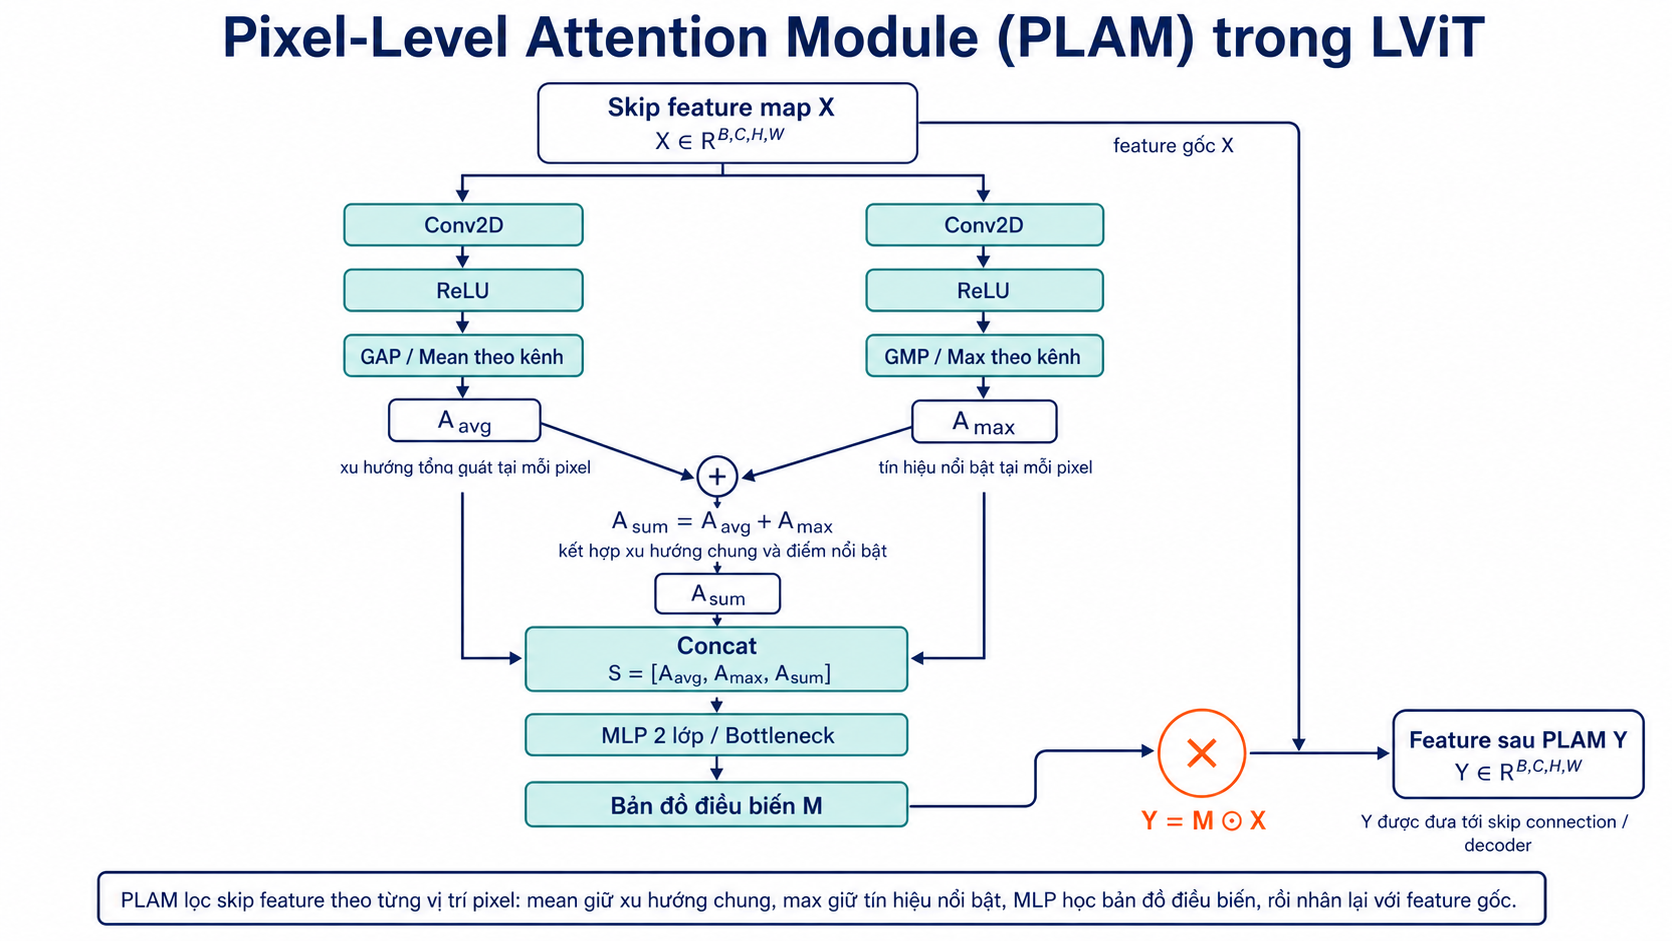
\includegraphics[width=\textwidth]{figures/lvit_plam_generated.png}
    \caption{Chi tiết mức điểm ảnh Attention Module (PLAM). Từ skip bản đồ đặc trưng \(X\), PLAM tạo hai nhánh thống kê theo kênh: trung bình để giữ xu hướng tổng quát và cực đại để giữ tín hiệu nổi bật. Ba bản đồ \(A_{avg}\), \(A_{max}\) và \(A_{sum}\) được ghép lại, đưa qua bottleneck/MLP để sinh bản đồ điều biến \(M\), sau đó nhân lại với đặc trưng gốc \(X\) để tạo đặc trưng đã điều biến \(Y\).}
    \label{fig:lvit-plam-generated}
\end{figure}

\subsection*{Nguyên lý}

Nguyên lý của PLAM là tạo một bản đồ điều biến theo vị trí từ chính bản đồ đặc trưng. Cho bản đồ đặc trưng:
\[
X\in\mathbb{R}^{B\times C\times H\times W}.
\]
Tại mỗi vị trí \((u,v)\), PLAM gom thông tin theo kênh bằng hai thống kê:
\[
A_{avg}(u,v)=\frac{1}{C}\sum_{c=1}^{C}X_{c,u,v},
\qquad
A_{max}(u,v)=\max_{c}X_{c,u,v}.
\]
Average phản ánh xu hướng tổng quát của các kênh, còn max phản ánh kênh nổi bật nhất tại vị trí đó. PLAM ghép thêm tổng của hai thống kê:
\[
S(u,v)=[A_{avg}(u,v), A_{max}(u,v), A_{avg}(u,v)+A_{max}(u,v)].
\]
Sau đó một bottleneck nhỏ học hàm \(g\) để tạo map điều biến \(M=g(S)\), rồi nhân lại với đặc trưng gốc:
\[
Y = M \odot X.
\]
Về trực giác, nếu một vị trí có tín hiệu cục bộ quan trọng, PLAM có thể tăng ảnh hưởng của nó trong skip connection; nếu vị trí ít liên quan, nó có thể bị giảm vai trò.

\subsection*{Phương pháp}

PLAM tạo hai nhánh xử lý cục bộ, sau đó lấy mean/max theo chiều kênh. Ba bản đồ \(\text{avg}\), \(\text{max}\), và \(\text{avg}+\text{max}\) được concatenate, chuyển chiều để đưa qua bottleneck tuyến tính, rồi kết quả được nhân với bản đồ đặc trưng gốc. Vì đầu ra được dùng như map điều biến theo điểm ảnh, báo cáo gọi nó là map điều biến/attention theo điểm ảnh thay vì khẳng định nó luôn là gate xác suất trong \([0,1]\).

Trong nhánh bộ giải mã, PLAM được dùng trước khi concatenate skip đặc trưng với đặc trưng đã upsample. Như vậy skip connection không còn là đường sao chép đặc trưng thô, mà là đường đặc trưng đã được lọc/điều biến theo mức quan trọng mức điểm ảnh.

\subsection*{Giải thuật}

Quy trình PLAM có thể viết bằng pseudo code như sau:

\begin{algorithm}[H]
\caption{Thuật toán Module chú ý mức điểm ảnh (PLAM)}
\label{alg:plam}
\begin{algorithmic}[1]
\Require Skip bản đồ đặc trưng \(X\in\mathbb{R}^{B\times C\times H\times W}\)
\Ensure bản đồ đặc trưng đã điều biến \(Y\)
\State \(X_{avg} \gets \mathrm{ReLU}(\mathrm{Conv1x1}_{avg}(X))\) \Comment{Nhánh thứ nhất học phép biến đổi cục bộ trước khi lấy thống kê trung bình.}
\State \(A_{avg} \gets \mathrm{MeanOverChannels}(X_{avg})\) \Comment{Tóm tắt mức kích hoạt trung bình tại mỗi điểm ảnh, phản ánh xu hướng chung của các kênh.}
\State \(A_{avg} \gets \mathrm{UnsqueezeChannel}(A_{avg})\) \Comment{Đưa bản đồ về dạng có chiều kênh để ghép với các bản đồ khác.}
\State \(X_{max} \gets \mathrm{ReLU}(\mathrm{Conv1x1}_{max}(X))\) \Comment{Nhánh thứ hai học phép biến đổi cục bộ trước khi lấy đáp ứng nổi bật nhất.}
\State \(A_{max} \gets \mathrm{MaxOverChannels}(X_{max})\) \Comment{Giữ tín hiệu mạnh nhất tại từng vị trí, hữu ích cho biên hoặc vùng nhỏ.}
\State \(A_{max} \gets \mathrm{UnsqueezeChannel}(A_{max})\) \Comment{Chuẩn hóa shape để có thể concatenate theo chiều kênh.}
\State \(A_{sum} \gets A_{avg}+A_{max}\) \Comment{Kết hợp xu hướng chung và tín hiệu nổi bật thành một bản đồ bổ sung.}
\State \(S \gets \mathrm{ConcatChannel}(A_{avg},A_{max},A_{sum})\) \Comment{Tạo mô tả mức điểm ảnh gồm ba góc nhìn: trung bình, cực đại và tổng.}
\State \(S \gets \mathrm{TransposeForLinear}(S)\) \Comment{Đổi trục tensor để bottleneck tuyến tính xử lý đúng chiều đặc trưng.}
\State \(M \gets \mathrm{BottleneckMLP}(S)\) \Comment{Học bản đồ điều biến theo vị trí từ ba thống kê mức điểm ảnh.}
\State \(M \gets \mathrm{TransposeBack}(M)\) \Comment{Đưa map điều biến trở lại cùng bố cục không gian với đặc trưng gốc.}
\State \(Y \gets M \odot X\) \Comment{Nhân theo từng vị trí/kênh để nhấn mạnh hoặc làm yếu skip đặc trưng trước bộ giải mã.}
\State \Return \(Y\) \Comment{đặc trưng sau PLAM vẫn giữ kích thước không gian, nhưng đã được điều biến theo mức quan trọng điểm ảnh.}
\end{algorithmic}
\end{algorithm}



Nếu xem skip connection là đường chuyển chi tiết từ bộ mã hóa sang bộ giải mã, PLAM giống một bộ lọc đặt trên đường đó. Với ảnh y khoa, mọi chi tiết cục bộ không quan trọng như nhau: có vùng nền, vùng giải phẫu bình thường, vùng nhiễu và vùng tổn thương. PLAM giúp bộ giải mã nhận được skip đặc trưng đã được nhấn mạnh theo vị trí, nhờ đó mặt nạ phục hồi tốt hơn ở biên và vùng nhỏ. Đây là lý do PLAM bổ sung hợp lý cho Transformer: attention lo quan hệ xa, còn PLAM bảo vệ tín hiệu mức điểm ảnh.

\section{EPI và LV loss trong học bán giám sát}

Mục này là phần nối giữa kiến trúc và bài toán ít nhãn. Nếu chỉ có dữ liệu có nhãn, LViT có thể học như một mô hình segmentation thông thường. Nhưng động lực lớn của LViT là ảnh y khoa thường thiếu mask chuyên gia. Vì vậy, mô hình cần học từ dữ liệu chưa nhãn mà không để nhãn giả sai làm hỏng quá trình học. EPI và LV loss là hai cơ chế của LViT cho mục tiêu đó: EPI làm ổn định pseudo-label theo thời gian, còn LV loss đưa văn bản vào quá trình kiểm soát học chưa nhãn.

\begin{figure}[H]
    \centering
    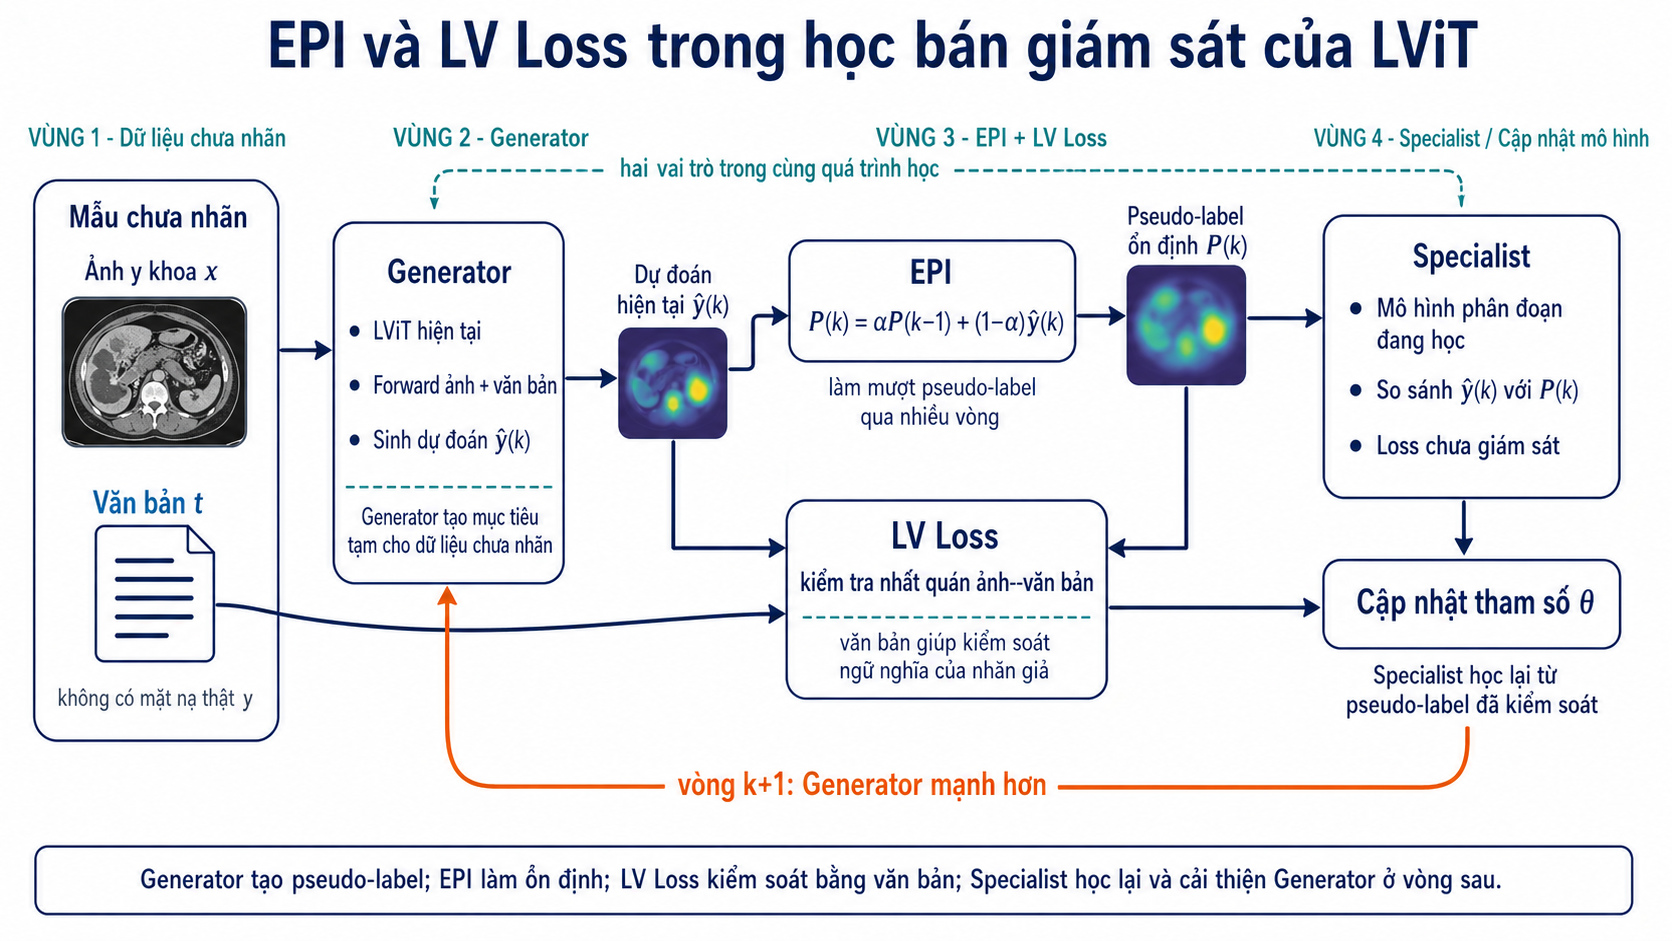
\includegraphics[width=\textwidth]{figures/lvit_epi_lv_loss_generated.png}
    \caption{Sự phối hợp giữa Generator và Specialist trong học bán giám sát của LViT. Generator là vai trò sinh pseudo-label từ mô hình hiện tại trên mẫu chưa nhãn; EPI làm ổn định pseudo-label qua nhiều vòng; LV loss dùng văn bản để kiểm soát tính nhất quán ảnh--văn bản; Specialist học lại từ pseudo-label đã kiểm soát để cập nhật tham số, làm Generator ở vòng sau mạnh hơn.}
    \label{fig:lvit-epi-lv-loss-generated}
\end{figure}

\begin{figure}[H]
    \centering
    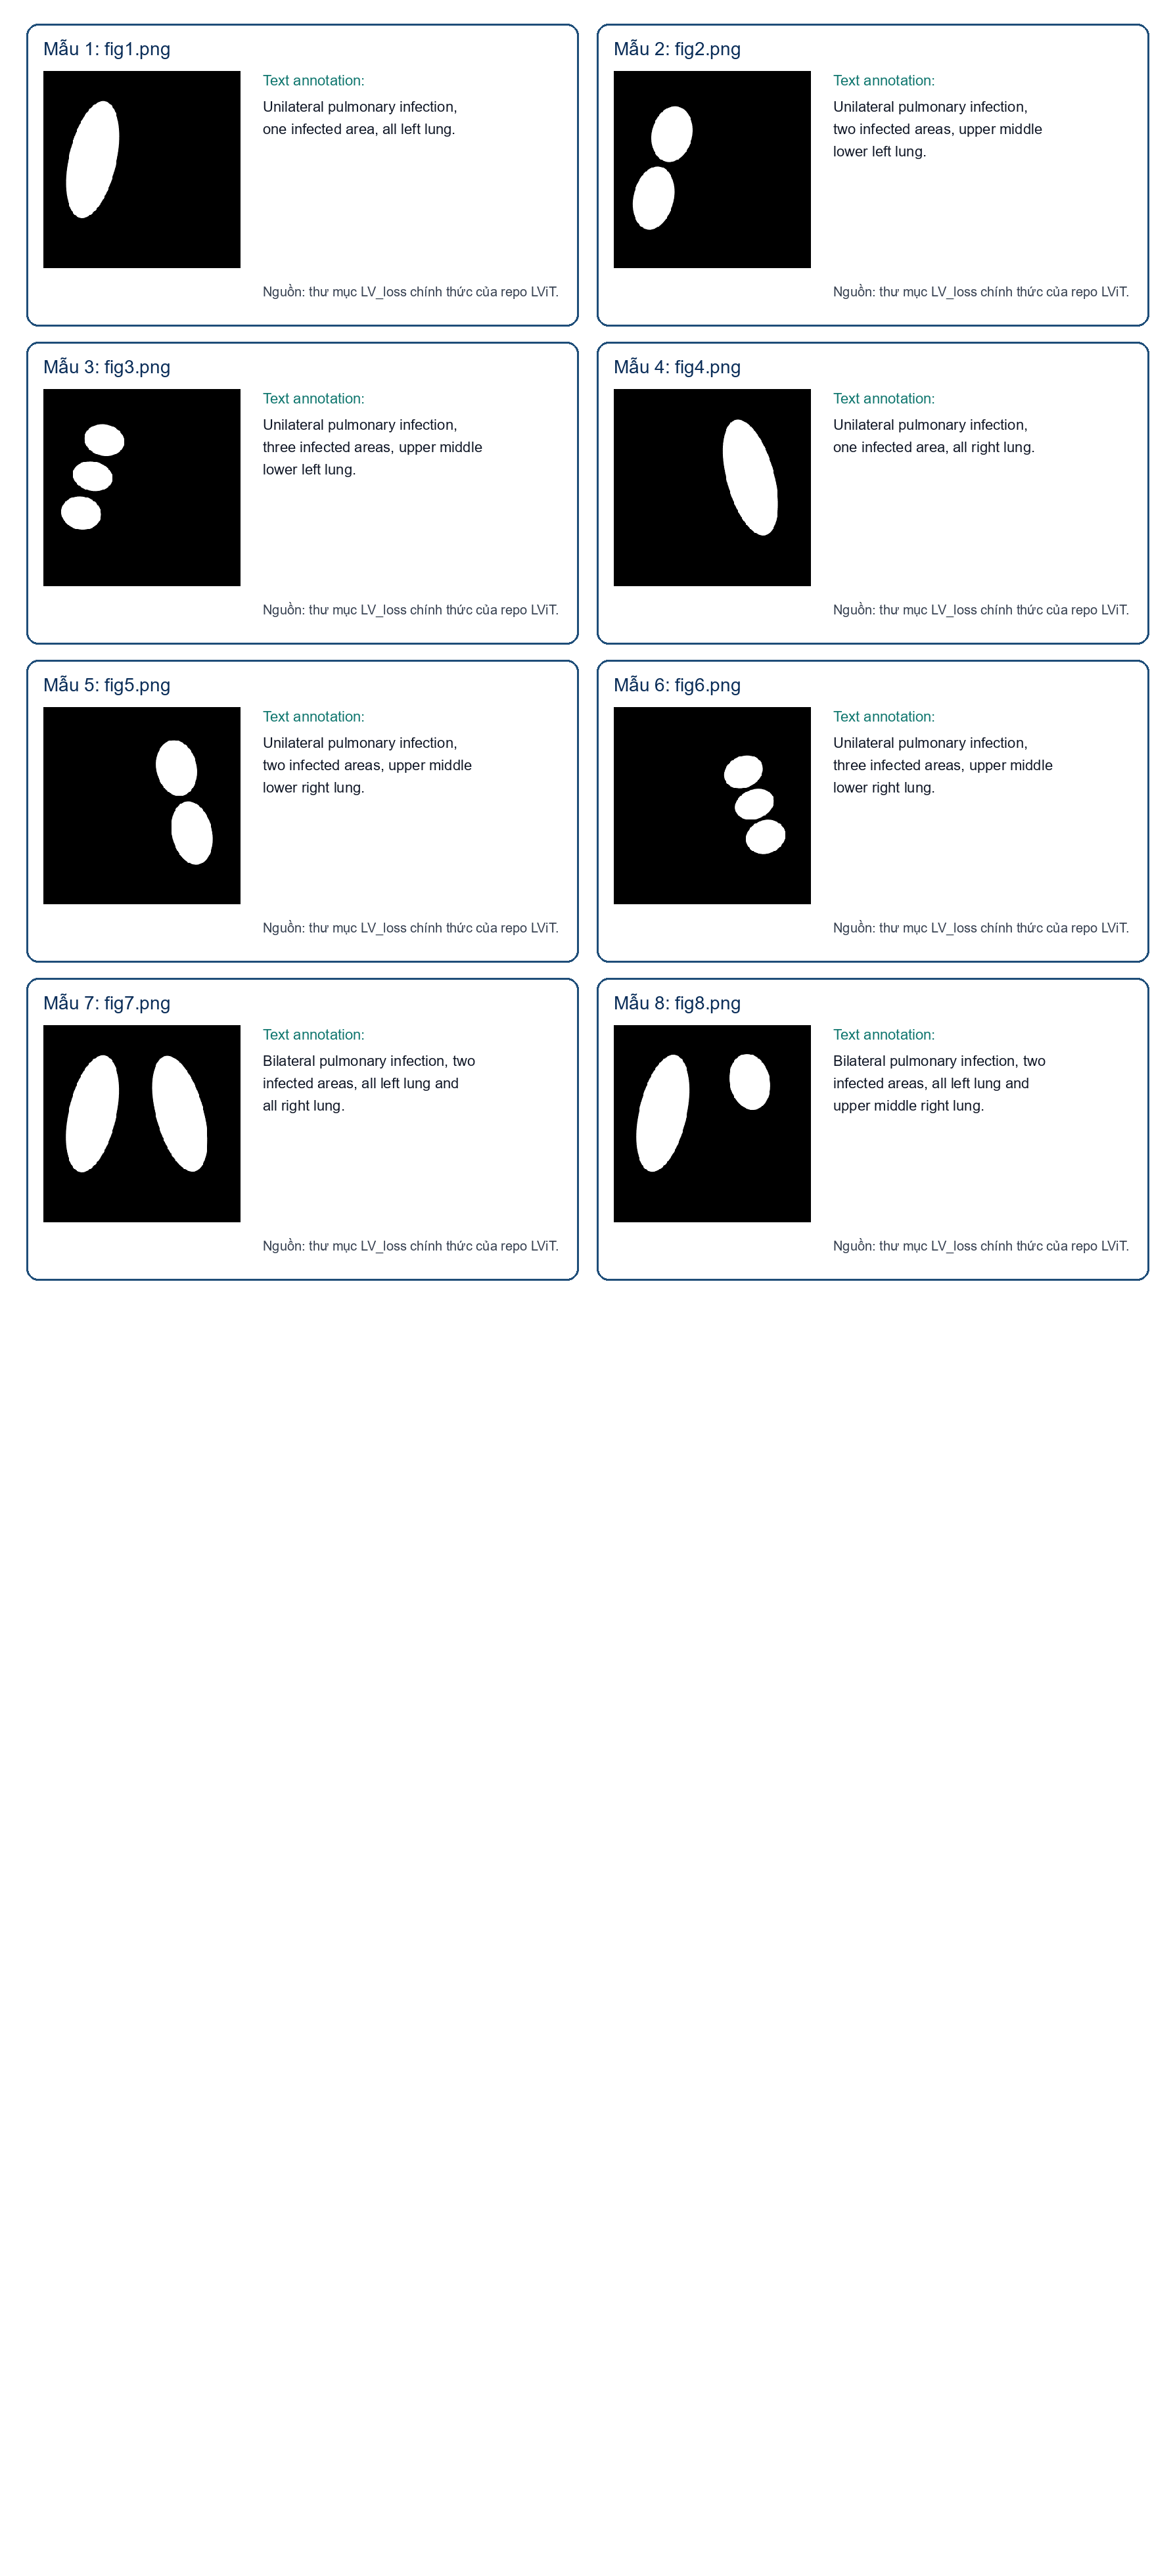
\includegraphics[width=0.95\textwidth]{figures/lvit_lvloss_prior_gallery_page1.png}
    \caption{Tám cặp \textit{contrastive label} đầu tiên do tác giả LViT công bố trong thư mục \texttt{LV\_loss/}. Mỗi cặp gồm một mask quy ước và một câu mô tả có cấu trúc, ví dụ phân biệt nhiễm một bên/hai bên, số vùng nhiễm, và vị trí thùy phổi trái/phải.}
    \label{fig:lvit-lvloss-prior-page1}
\end{figure}

\begin{figure}[H]
    \centering
    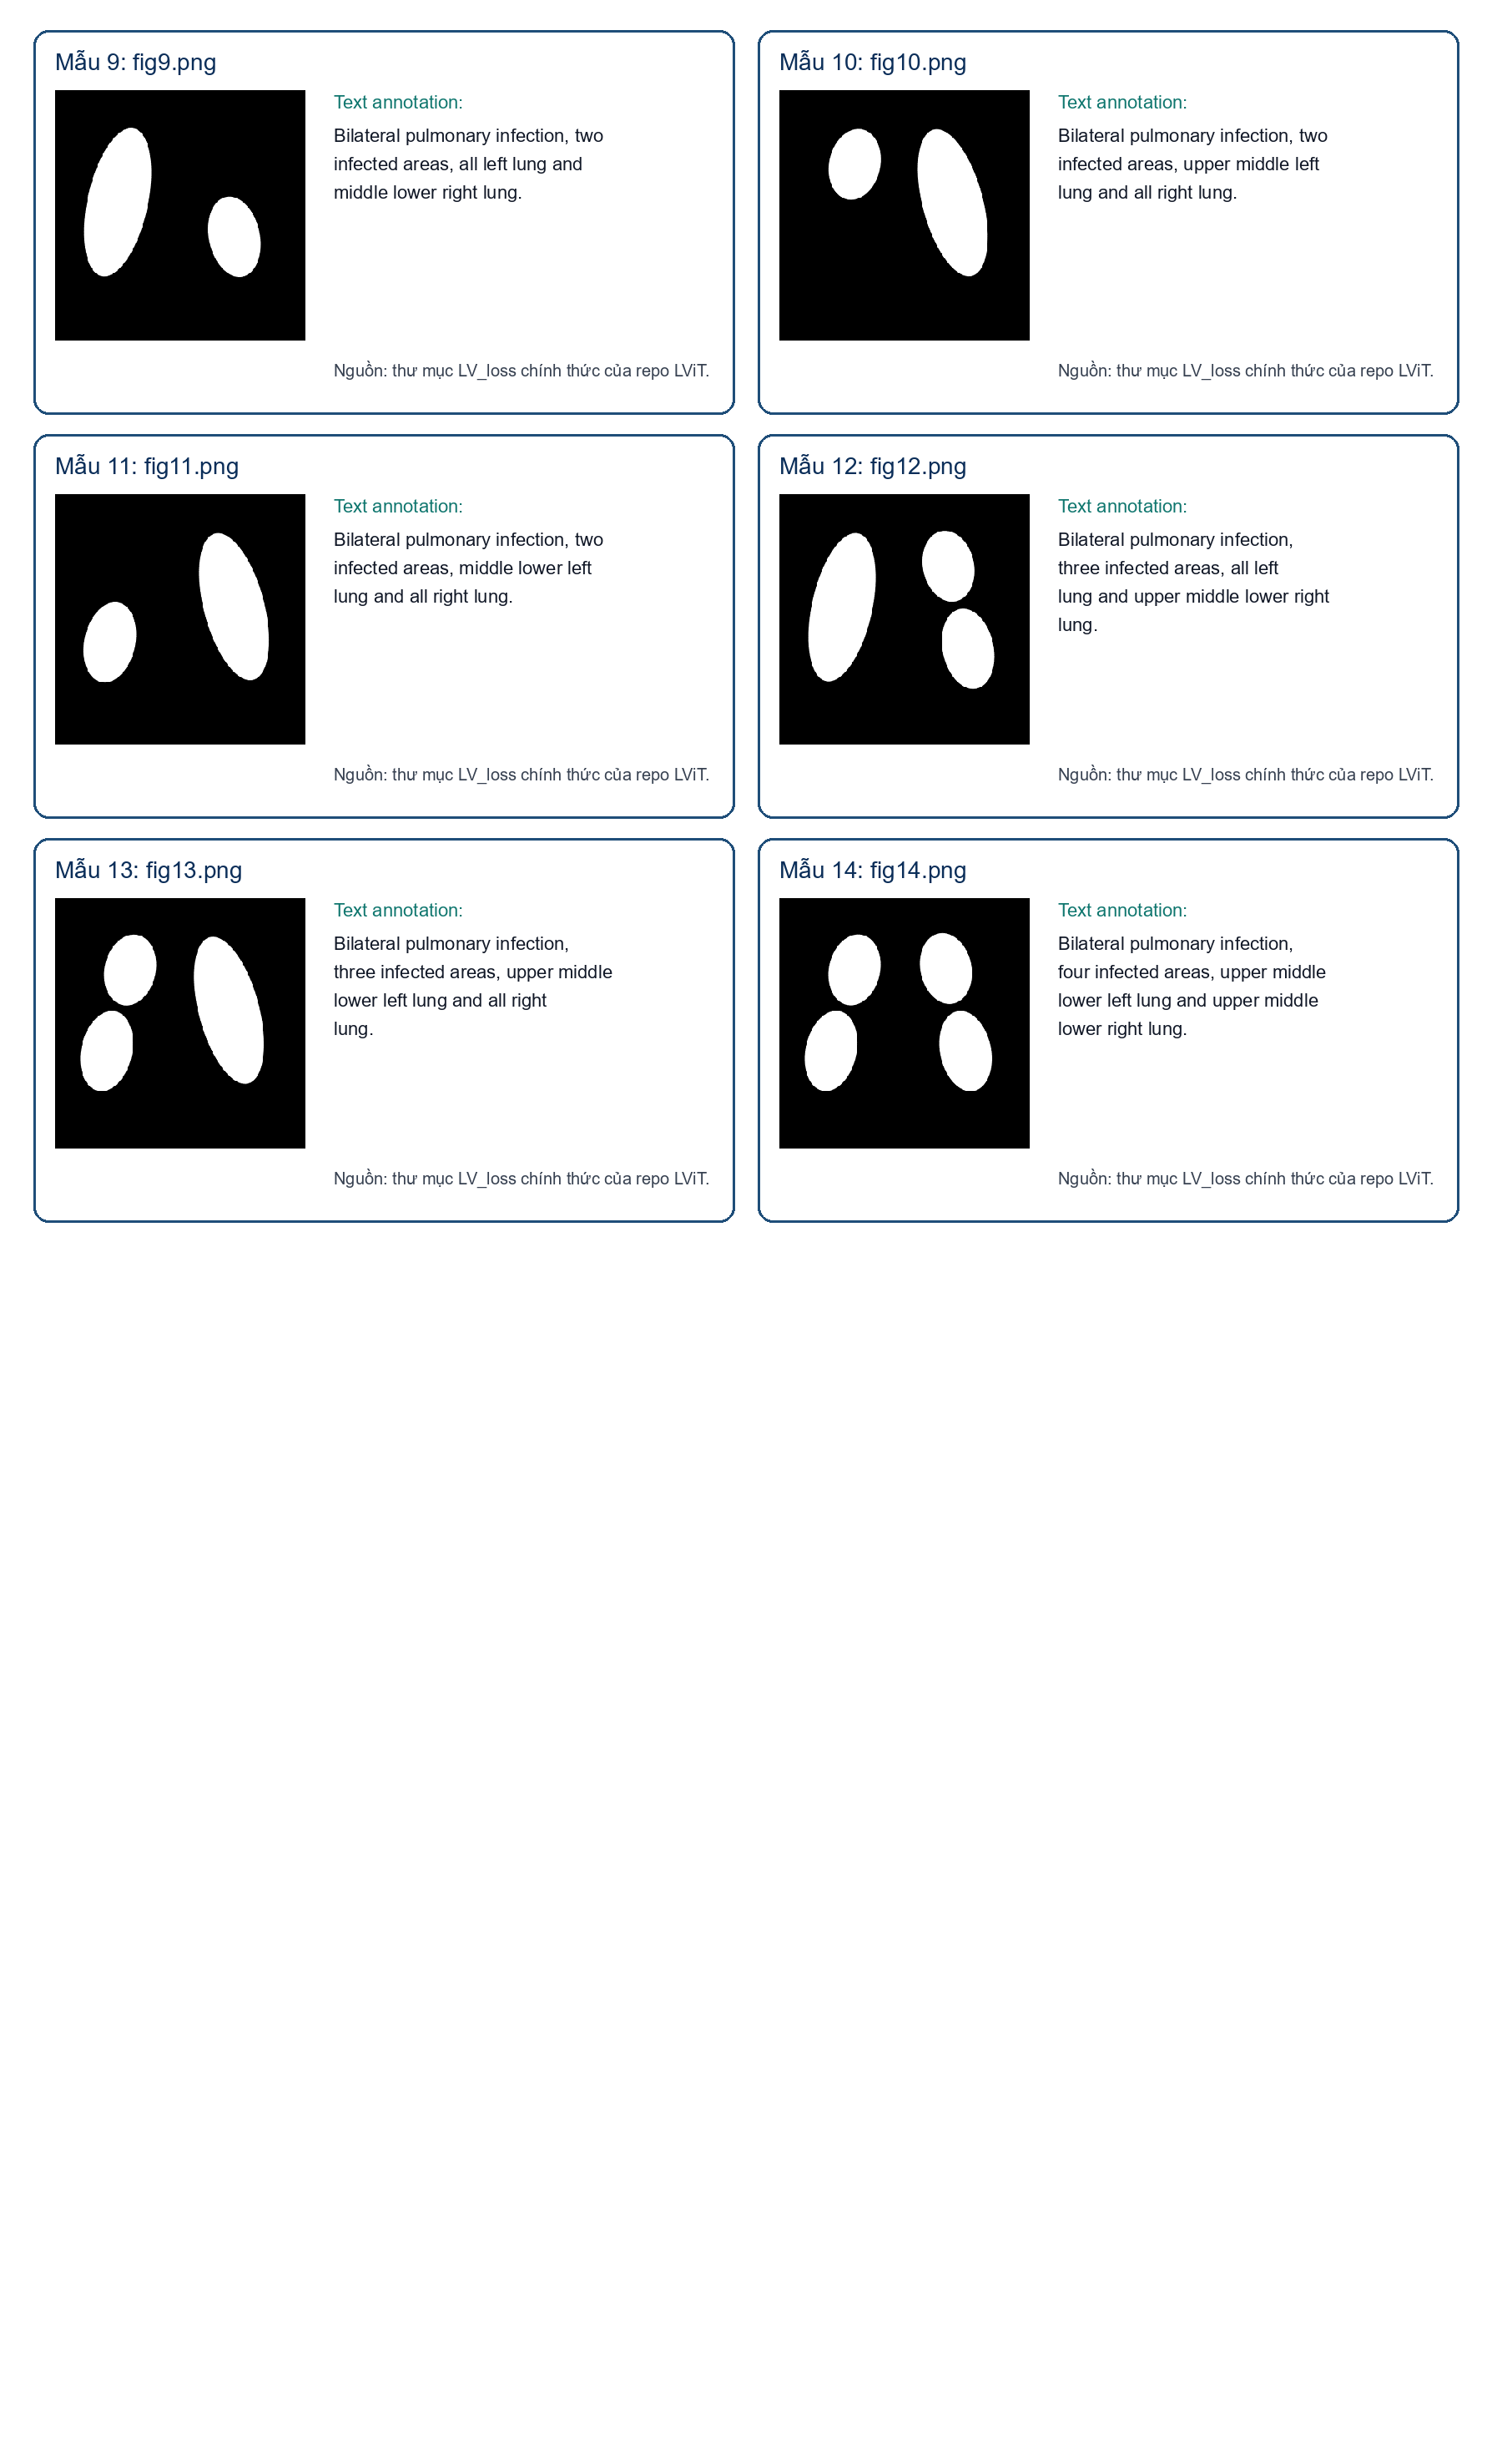
\includegraphics[width=0.95\textwidth]{figures/lvit_lvloss_prior_gallery_page2.png}
    \caption{Sáu cặp \textit{contrastive label} còn lại trong bộ prior knowledge của \texttt{LV\_loss/}. Hai hình này cộng lại hiển thị toàn bộ 14 cặp ảnh--text mà nhóm tác giả LViT phát hành để phục vụ LV loss.}
    \label{fig:lvit-lvloss-prior-page2}
\end{figure}

\subsection*{Nguyên lý}

Với mẫu chưa nhãn \((x,t)\), không tồn tại \(y\) để so sánh trực tiếp. Mô hình chỉ có thể tạo dự đoán:
\[
\hat{Y}^{(k)} = f_{\theta^{(k)}}(x,t),
\]
tại epoch hoặc vòng lặp \(k\). Nếu dùng ngay \(\hat{Y}^{(k)}\) làm nhãn giả, mô hình có thể học theo nhiễu tức thời. EPI giải quyết bằng cách dùng trung bình mũ theo thời gian:
\[
P^{(k)}=\alpha P^{(k-1)} + (1-\alpha)\hat{Y}^{(k)}.
\]
Trong đó \(P^{(k)}\) là pseudo-label tích lũy, \(\alpha\) là hệ số giữ lại thông tin quá khứ. Paper LViT mô tả hệ số lớn, ví dụ \(\alpha=0.99\), để pseudo-label thay đổi chậm hơn dự đoán từng epoch \cite{li2023lvit}. EPI vì thế là cơ chế làm mượt theo \emph{thời gian}: nó lấy lịch sử dự đoán của chính mẫu hiện tại để giảm tác động của nhiễu nhất thời.

LV loss của LViT lại giải một việc khác. Tác giả không chỉ nói chung rằng ``văn bản nên hướng dẫn mask'', mà xây sẵn một bộ \emph{prior knowledge} hữu hạn trong thư mục \texttt{LV\_loss/}. Bộ này gồm 14 cặp \((t_c,Y_c)\), trong đó \(t_c\) là một câu mô tả có cấu trúc và \(Y_c\) là mask quy ước đi kèm. Các câu mô tả xoay quanh ba trục ngữ nghĩa ổn định: nhiễm một bên hay hai bên, có bao nhiêu vùng nhiễm, và các vùng đó nằm ở bên trái/phải hay ở mức trên--giữa--dưới của phổi. Hai Hình~\ref{fig:lvit-lvloss-prior-page1} và~\ref{fig:lvit-lvloss-prior-page2} hiển thị toàn bộ 14 cặp mà tác giả công bố.

Từ bank prior này, LViT dùng \emph{hai tầng cosine similarity}. Tầng thứ nhất đo độ giống nhau giữa văn bản của mẫu chưa nhãn và các câu prior:
\[
\mathrm{TextSim}(t_p,t_c)=
\frac{x_{text,p}\cdot x_{text,c}}
{\|x_{text,p}\|\,\|x_{text,c}\|}.
\]
Prior có \(\mathrm{TextSim}\) lớn nhất được chọn làm \emph{contrastive label}. Tầng thứ hai không so văn bản nữa mà so chính pseudo-label hiện tại với mask prior tương ứng:
\[
\mathrm{ImgSim}(\hat{Y}^{(k)},Y_c)=
\frac{x_{img,p}\cdot x_{img,c}}
{\|x_{img,p}\|\,\|x_{img,c}\|},
\qquad
\mathcal{L}_{LV}=1-\mathrm{ImgSim}.
\]
Nói ngắn gọn, EPI ổn định pseudo-label theo thời gian, còn LV loss kiểm tra xem pseudo-label đó có còn nhất quán với một cấu hình nhiễm phổi gần nghĩa nhất trong bank prior hay không.

\subsection*{Phương pháp}

Ở mức phương pháp, học bán giám sát của LViT gồm hai đường song song nhưng không đồng nhất. Đường thứ nhất là đường thị giác theo thời gian: mô hình forward ảnh--văn bản để tạo \(\hat{Y}^{(k)}\), rồi EPI cập nhật pseudo-label \(P^{(k)}\) bằng trung bình mũ qua các vòng lặp. Đường thứ hai là đường đối chiếu ảnh--văn bản: văn bản chú thích của mẫu chưa nhãn được so với 14 câu prior để chọn ra \emph{contrastive text} gần nhất; sau đó mô hình lấy mask prior tương ứng làm \emph{contrastive label} và so nó với pseudo-label hiện tại bằng cosine similarity ở không gian ảnh.

Loss chưa nhãn có thể được diễn giải ở dạng tổng quát:
\[
\mathcal{L}_{u}
=
\mathcal{L}_{seg}(\hat{Y},P)
+ \gamma \mathcal{L}_{LV}(t,\hat{Y},P),
\]
trong đó \(\mathcal{L}_{seg}\) là loss phân đoạn giữa dự đoán và pseudo-label đã được EPI làm mượt, còn \(\mathcal{L}_{LV}\) là thành phần đối chiếu với contrastive label lấy từ bank prior. Paper nhấn mạnh rằng contrastive label chủ yếu cung cấp thông tin vị trí gần đúng, không tinh chỉnh biên chi tiết, nên LV loss chỉ nên đóng vai trò \emph{bổ sung} để tránh các ca lệch ngữ nghĩa lớn, chứ không thay thế BCE/Dice. Trong triển khai gốc, loss chưa nhãn vì thế được viết thành BCE có trọng số \(+\) Dice có trọng số \(+\;0.1\times LV\_loss\).

\subsection*{Giải thuật}

Quy trình EPI/LV loss cho dữ liệu chưa nhãn có thể viết bằng pseudo code như sau:

\begin{algorithm}[H]
\caption{EPI và LV loss cho mẫu chưa nhãn}
\label{alg:epi-lv}
\begin{algorithmic}[1]
\Require Mẫu chưa nhãn \((x,t)\), tham số \(\theta\), pseudo-label cũ \(P_{prev}\), bank prior \(\mathcal{B}=\{(t_c,Y_c)\}_{c=1}^{14}\), hệ số \(\alpha\), trọng số \(\gamma\)
\Ensure Pseudo-label mới \(P_{curr}\), contrastive label \(Y_{c^\star}\), loss chưa nhãn \(\mathcal{L}_{u}\)
\State \(x_p \gets \mathrm{PreprocessImage}(x)\) \Comment{Chuẩn hóa ảnh chưa nhãn giống ảnh có nhãn để mô hình nhận cùng phân bố.}
\State \(e_t \gets \mathrm{EncodeText}(t)\) \Comment{Văn bản là tín hiệu ngữ nghĩa duy nhất còn lại khi không có mask chuyên gia.}
\State \(\hat{Y} \gets \mathrm{LViT}(x_p,e_t;\theta)\) \Comment{Dự đoán hiện tại của mô hình, dùng làm nguồn tạo pseudo-label.}
\State \(\hat{Y}_{stop} \gets \mathrm{Detach}(\hat{Y})\) \Comment{Ngắt gradient để pseudo-label đóng vai trò mục tiêu tạm thời, không bị cập nhật trực tiếp.}
\If{\(P_{prev}=\varnothing\)}
  \State \(P_{curr} \gets \hat{Y}_{stop}\) \Comment{Nếu chưa có bộ nhớ trước đó, dùng dự đoán hiện tại làm pseudo-label khởi tạo.}
\Else
  \State \(P_{curr} \gets \alpha P_{prev} + (1-\alpha)\hat{Y}_{stop}\) \Comment{EPI lấy trung bình mũ để pseudo-label biến đổi chậm và ổn định hơn.}
\EndIf
\For{mỗi cặp prior \((t_c,Y_c)\in\mathcal{B}\)}
  \State \(s_c \gets \mathrm{CosineSim}(\mathrm{EncodeText}(t),\mathrm{EncodeText}(t_c))\) \Comment{So văn bản mẫu hiện tại với từng mô tả prior để tìm ca gần nghĩa nhất.}
\EndFor
\State \(c^\star \gets \arg\max_c s_c\) \Comment{Chọn prior có cosine similarity lớn nhất trong không gian văn bản.}
\State \(Y_{c^\star} \gets \mathrm{MaskPrior}(c^\star)\) \Comment{Lấy contrastive label đi kèm với mô tả prior gần nhất.}
\State \(P_{target} \gets \mathrm{PreparePseudoTarget}(P_{curr})\) \Comment{Có thể giữ dạng xác suất mềm hoặc ngưỡng hóa tùy thiết lập huấn luyện.}
\State \(\mathcal{L}_{BCE} \gets \mathrm{BCELoss}(\hat{Y},P_{target})\) \Comment{Ép xác suất điểm ảnh hiện tại nhất quán với pseudo-label.}
\State \(\mathcal{L}_{Dice} \gets \mathrm{DiceLoss}(\hat{Y},P_{target})\) \Comment{Giữ ràng buộc mức vùng để pseudo-mask không chỉ đúng từng điểm ảnh rời rạc.}
\State \(\mathcal{L}_{seg} \gets \mathcal{L}_{BCE}+\mathcal{L}_{Dice}\) \Comment{Loss phân đoạn chưa nhãn dùng pseudo-label thay cho mask thật.}
\State \(v_p \gets \mathrm{Vectorize}(P_{curr})\), \(v_c \gets \mathrm{Vectorize}(Y_{c^\star})\) \Comment{Biến pseudo-label và contrastive label thành vector để so tương đồng bố cục nhiễm.}
\State \(\mathrm{ImgSim} \gets \mathrm{CosineSim}(v_p,v_c)\) \Comment{Độ giống nhau cosine giữa pseudo-label hiện tại và mask prior đã chọn.}
\State \(\mathcal{L}_{LV} \gets 1-\mathrm{ImgSim}\) \Comment{Nếu pseudo-label lệch xa prior gần nghĩa nhất, LV loss tăng để phạt.}
\State \(\mathcal{L}_{u} \gets \mathcal{L}_{seg}+\gamma\mathcal{L}_{LV}\) \Comment{Tín hiệu học chưa nhãn gồm nhất quán mask giả và ràng buộc ảnh--văn bản.}
\State \Return \(P_{curr},Y_{c^\star},\mathcal{L}_{u}\) \Comment{Pseudo-label mới được lưu cho vòng lặp sau; contrastive label và loss dùng để giám sát nhánh chưa nhãn.}
\end{algorithmic}
\end{algorithm}



Có thể hiểu EPI như một bộ nhớ chậm của pseudo-label: một dự đoán nhiễu ở epoch hiện tại không lập tức trở thành mục tiêu huấn luyện mạnh, vì nó chỉ chiếm tỉ lệ nhỏ trong \(P^{(k)}\). Còn LV loss là một cơ chế kiểm tra \emph{đối chiếu}: nó không hỏi ``mask này có đúng tuyệt đối không'', mà hỏi ``mask này có còn hợp với một mẫu prior có mô tả văn bản gần nhất hay không''. Vì bộ prior knowledge của LViT chỉ mã hóa bố cục nhiễm ở mức gần đúng, LV loss chủ yếu ngăn các trường hợp lệch lớn về phía trái/phải, một bên/hai bên, hoặc số vùng nhiễm; nó không thay thế loss biên mịn của phân đoạn. Hai cơ chế này vì thế bổ sung cho nhau: EPI làm ổn định theo thời gian, LV loss làm nhất quán theo ngữ nghĩa ảnh--văn bản.

\section{Hàm mất mát và độ đo}

Mục cuối của Chương 3 làm rõ mô hình học bằng gì và được đánh giá bằng gì. Đây là điểm thường bị viết thiếu trong báo cáo: nếu chỉ mô tả kiến trúc mà không nói đầu ra xác thực, loss và metric, người đọc không biết tham số mạng được tối ưu theo tín hiệu nào. Với LViT, loss phải xử lý hai mức: mức điểm ảnh foreground/background và vùng phân đoạn tổng thể.

\subsection*{Nguyên lý}

Trong phân đoạn nhị phân, mỗi điểm ảnh có xác suất thuộc foreground. Về bản chất, BCE đo sai số từng điểm ảnh:
\[
\mathcal{L}_{BCE}
=-\frac{1}{N}\sum_{p}
\left[
y_p\log(\hat{y}_p)
+(1-y_p)\log(1-\hat{y}_p)
\right].
\]
BCE phù hợp để học xác suất điểm ảnh, nhưng nếu foreground nhỏ, mô hình có thể đạt loss thấp bằng cách dự đoán nhiều nền. Dice loss bổ sung góc nhìn theo vùng:
\[
\mathcal{L}_{Dice}
=1-\frac{2\sum_p y_p\hat{y}_p+\epsilon}
{\sum_p y_p+\sum_p\hat{y}_p+\epsilon}.
\]
Dice loss trực tiếp khuyến khích vùng dự đoán chồng lên vùng thật, nên gần hơn với mục tiêu đánh giá segmentation. Tuy nhiên, triển khai chính thức của LViT không dùng đúng hai công thức cơ sở này theo dạng thuần, mà chuyển chúng thành \emph{weighted BCE} và \emph{weighted Dice} để giảm ảnh hưởng của mất cân bằng foreground/background trong ảnh y khoa.

\subsection*{Phương pháp}

Các thành phần loss chính gồm BCE có trọng số, Dice loss có trọng số, loss kết hợp cho dữ liệu có nhãn và loss kết hợp cho dữ liệu chưa nhãn. Trong mã nguồn chính thức, lớp \texttt{WeightedDiceBCE} kết hợp \texttt{WeightedBCE(weights=[0.5,0.5])} và \texttt{WeightedDiceLoss(weights=[0.5,0.5])}; còn lớp \texttt{WeightedDiceBCE\_unsup} giữ nguyên hai thành phần này và cộng thêm \(0.1\times LV\_loss\). Vì vậy, ở mức triển khai, với dữ liệu có nhãn ta có:
\[
\mathcal{L}_{sup}
=w_D\mathcal{L}_{Dice}
+w_B\mathcal{L}_{BCE}.
\]
Cấu hình huấn luyện thường dùng trọng số Dice và BCE bằng nhau, cụ thể \(w_D=w_B=0.5\). Với dữ liệu chưa nhãn, loss bổ sung thêm \(0.1\times LV\_loss\):
\[
\mathcal{L}_{unsup}
=w_D\mathcal{L}_{Dice}
+w_B\mathcal{L}_{BCE}
+0.1\mathcal{L}_{LV}.
\]
Cách kết hợp này làm rõ vai trò từng thành phần: weighted BCE giữ tín hiệu điểm ảnh-wise, weighted Dice giữ tín hiệu chồng lấn vùng, còn LV loss chỉ đóng vai trò ràng buộc ngữ nghĩa bổ sung trên nhánh chưa nhãn.

\subsection*{Giải thuật}

Quy trình tính loss và metric có thể viết bằng pseudo code như sau:

\begin{algorithm}[H]
\caption{Tính loss huấn luyện và metric đánh giá}
\label{alg:loss-metrics}
\begin{algorithmic}[1]
\Require Dự đoán \(\hat{y}\), mask chuyên gia \(y\) nếu có, pseudo-label \(P\) nếu có, LV loss nếu có, ngưỡng \(\tau\), chế độ \(\mathrm{mode}\)
\Ensure Loss huấn luyện \(\mathcal{L}\) nếu có, metric Dice/IoU nếu đánh giá
\State \(\mathcal{L} \gets \varnothing,\; \mathrm{metrics} \gets \varnothing\) \Comment{Khởi tạo rỗng vì không phải chế độ nào cũng cần cả loss và metric.}
\If{\(\mathrm{mode}=\mathrm{labeled}\)}
  \State \(y_p \gets \mathrm{PreprocessMask}(y)\) \Comment{Mặt nạ chuyên gia là đầu ra xác thực dùng cho học có giám sát.}
  \State \(bce \gets \mathrm{WeightedBCE}(\hat{y},y_p)\) \Comment{Đo sai khác xác suất theo từng điểm ảnh.}
  \State \(dice \gets \mathrm{WeightedDiceLoss}(\hat{y},y_p)\) \Comment{Đo sai khác theo mức chồng lấn vùng phân đoạn.}
  \State \(\mathcal{L} \gets w_{bce}bce+w_{dice}dice\) \Comment{Loss có giám sát kết hợp điểm ảnh-wise và region-wise objectives.}
\EndIf
\If{\(\mathrm{mode}=\mathrm{unlabeled}\)}
  \State \(P_t \gets \mathrm{PreparePseudoTarget}(P)\) \Comment{Pseudo-label là mục tiêu tạm, được tạo từ dự đoán/EPI chứ không phải mask chuyên gia.}
  \State \(bce \gets \mathrm{WeightedBCE}(\hat{y},P_t)\) \Comment{Khuyến khích dự đoán nhất quán với pseudo-label ở từng điểm ảnh.}
  \State \(dice \gets \mathrm{WeightedDiceLoss}(\hat{y},P_t)\) \Comment{Giữ hình dạng vùng dự đoán gần pseudo-mask đã ổn định.}
  \State \(\mathcal{L} \gets w_{bce}bce+w_{dice}dice+\gamma\mathcal{L}_{LV}\) \Comment{Bổ sung LV loss để văn bản kiểm soát học chưa nhãn.}
\EndIf
\If{\(\mathrm{mode}=\mathrm{evaluation}\)}
  \State \(\hat{y}_{bin} \gets \mathrm{Threshold}(\hat{y},\tau)\) \Comment{Chuyển xác suất thành mặt nạ nhị phân để so với ground truth.}
  \State \(y_p \gets \mathrm{PreprocessMask}(y)\) \Comment{Ground truth chỉ dùng cho đánh giá sau khi dự đoán đã hoàn tất.}
  \State \(dice_m \gets \mathrm{DiceMetric}(\hat{y}_{bin},y_p)\) \Comment{Dice đo mức chồng lấn, nhạy với foreground nhỏ trong ảnh y khoa.}
  \State \(iou_m \gets \mathrm{IoUMetric}(\hat{y}_{bin},y_p)\) \Comment{IoU nghiêm hơn Dice vì mẫu số là hợp của vùng dự đoán và vùng thật.}
  \State \(\mathrm{metrics} \gets \{\mathrm{Dice}:dice_m,\mathrm{IoU}:iou_m\}\) \Comment{Metric dùng để báo cáo hiệu suất, không dùng để cập nhật tham số.}
\EndIf
\State \Return \(\mathcal{L},\mathrm{metrics}\) \Comment{Ở chế độ học trả về loss; ở chế độ đánh giá trả về Dice/IoU.}
\end{algorithmic}
\end{algorithm}



Dice và IoU được tính như sau:
\[
\mathrm{Dice}=\frac{2|Y\cap \hat{Y}|}{|Y|+|\hat{Y}|},
\qquad
\mathrm{IoU}=\frac{|Y\cap \hat{Y}|}{|Y\cup \hat{Y}|}.
\]
Dice thường dễ đọc hơn trong y khoa vì nó nhấn mạnh phần chồng lấn giữa hai vùng, đặc biệt khi foreground nhỏ. IoU nghiêm khắc hơn vì mẫu số là hợp của vùng thật và vùng dự đoán. Nếu một mô hình dự đoán lan quá rộng, IoU giảm rõ; nếu bỏ sót vùng thật, cả Dice và IoU đều giảm. Vì vậy, khi đọc kết quả LViT, cần nhìn cả Dice, IoU và chi phí tính toán. LViT có nhiều khối hơn U-Net do thêm Transformer, văn bản branch, PLAM và học bán giám sát; phần tăng chi phí này là đánh đổi để nhận lại ngữ cảnh xa và tín hiệu văn bản.

\chapter{Cài đặt và thử nghiệm}
\label{sec:experiment}

Chương này chuyển phần phương pháp ở Chương 3 thành một quy trình cài đặt và thử nghiệm có thể kiểm tra được. Tinh thần của chương là không chỉ nói mô hình gồm những khối nào, mà phải trả lời bốn câu hỏi thực nghiệm: thử nghiệm nhằm kiểm chứng điều gì, chạy trong điều kiện nào, dữ liệu và ground truth được dùng ra sao, và kết quả đo bằng tiêu chí nào. Phần cải tiến được chốt kết quả trước, sau đó mới đi vào môi trường, dữ liệu, quy trình và ablation để người đọc thấy rõ cải tiến có tạo ra thay đổi đo được hay không.

\section{Mục đích thử nghiệm}

Phần thực nghiệm có vai trò nối Chương 3 với bằng chứng đo được. Nếu Chương 3 giải thích LViT hoạt động bằng các khối ảnh--văn bản, Double-U, PLAM, EPI và LV loss, thì Chương 4 trả lời câu hỏi thực tế hơn: khi đặt các khối đó vào dữ liệu thật, mô hình có phân đoạn tốt hơn không, tốt hơn trong điều kiện nào, và phần cải tiến có tạo ra thay đổi ổn định hay chỉ là một cấu hình may mắn. Triết lý của phần thử nghiệm vì vậy là đặt kết quả định lượng lên trước, sau đó mới phân tích môi trường, dữ liệu, quy trình và ablation để giải thích vì sao kết quả đó đáng tin.

Kết quả chính cần chốt ngay là: trên QaTa-COV19, cấu hình cải tiến \textbf{QaTaLViT} vượt baseline trong cả ba mức tỉ lệ nhãn 25\%, 50\% và 100\%. Test Dice/IoU lần lượt đạt \(82.22/73.35\), \(84.03/75.62\) và \(85.28/77.25\). So với baseline trong bảng ablation, mức tăng Dice lần lượt là \(+3.80\), \(+3.71\) và \(+2.52\) điểm phần trăm; mức tăng IoU lần lượt là \(+4.92\), \(+5.02\) và \(+3.47\) điểm phần trăm. Đây là tín hiệu quan trọng vì cải tiến có hiệu quả mạnh nhất ở 25\% và 50\% nhãn, đúng với động lực ban đầu của LViT: khi mask chuyên gia ít, văn bản, pseudo-label và cơ chế kiểm soát nhãn giả có giá trị hơn.

Mục tiêu thứ nhất của thử nghiệm là \textbf{tái hiện vai trò của LViT như một mô hình phân đoạn ảnh--văn bản}. Báo cáo không chỉ muốn chạy một mô hình segmentation bất kỳ, mà muốn kiểm tra đúng tinh thần LViT: ảnh cung cấp bằng chứng thị giác, văn bản cung cấp ngữ nghĩa lâm sàng, còn mặt nạ chuyên gia cung cấp giám sát mức điểm ảnh khi có. Vì vậy, các thử nghiệm phải luôn theo dõi ba phần: dữ liệu ảnh, văn bản chú thích và ground truth mask.

Mục tiêu thứ hai là \textbf{đánh giá trong điều kiện nhãn hạn chế}. Đây là bối cảnh gần với y khoa thực tế hơn so với giả định mọi ảnh đều có mask đầy đủ. Khi chỉ dùng 25\% hoặc 50\% nhãn, mô hình phải tận dụng tốt hơn các mẫu chưa nhãn và thông tin văn bản. Nếu cải tiến chỉ tốt ở 100\% nhãn thì đóng góp về bán giám sát chưa thật thuyết phục; ngược lại, kết quả tăng rõ ở 25\% và 50\% nhãn cho thấy hướng cải tiến đi đúng vấn đề mà LViT đặt ra.

Mục tiêu thứ ba là \textbf{phân tích từng nhóm thay đổi bằng ablation}. Một kết quả cuối cùng cao hơn baseline chưa đủ để kết luận vì không biết phần nào tạo ra cải thiện. Do đó, Chương 4 tách các nhóm yếu tố như chuẩn hóa prompt, biểu diễn văn bản, prior không gian, fusion, kiểm soát pseudo-label, learning rate và augmentation. Cách làm này giúp phân biệt giữa cải tiến phương pháp và thay đổi do cấu hình huấn luyện.

Mục tiêu thứ tư là \textbf{kiểm tra khả năng chuyển miền dữ liệu}. QaTa-COV19 là dữ liệu X-quang, còn MosMedData+ là dữ liệu CT. Hai miền ảnh này khác nhau về cấu trúc không gian, độ tương phản, hình thái tổn thương và cách văn bản chú thích phản ánh bệnh. Vì vậy, MosMedData+ được dùng như một phép kiểm tra khó hơn: cùng triết lý ảnh--văn bản của LViT có còn hợp lý khi chuyển từ X-quang 2D sang lát CT hay không.

Từ các mục tiêu trên, phần thử nghiệm tập trung trả lời bốn câu hỏi:
\begin{enumerate}[label=(\arabic*)]
  \item LViT và biến thể cải tiến có cải thiện Dice/IoU so với baseline trong cùng điều kiện dữ liệu hay không?
  \item Cải thiện có rõ hơn khi tỉ lệ nhãn giảm xuống 25\% và 50\% hay không?
  \item văn bản chú thích, pseudo-label và các bước kiểm soát nhãn giả đóng góp thế nào vào hiệu quả cuối?
  \item Khi chuyển sang MosMedData+, yếu tố nào trở thành nút thắt: bộ mã hóa văn bản, tiền xử lý ảnh, augmentation, threshold hay cơ chế học chưa nhãn?
\end{enumerate}

\begin{table}[H]
  \centering
  \caption{Kết quả chính của cải tiến QaTaLViT trên QaTa-COV19. Giá trị là test Dice/IoU, đơn vị phần trăm.}
  \label{tab:qatalvit-main-results}
  \scriptsize
  \renewcommand{\arraystretch}{1.12}
  \setlength{\tabcolsep}{5pt}
  \begin{tabularx}{\textwidth}{@{}l Y Y Y@{}}
    \toprule
    Mô hình & 25\% nhãn & 50\% nhãn & 100\% nhãn \\
    \midrule
    Baseline trong ablation & 78.42 / 68.43 & 80.32 / 70.60 & 82.76 / 73.78 \\
    QaTaLViT cải tiến & 82.22 / 73.35 & 84.03 / 75.62 & 85.28 / 77.25 \\
    Mức tăng Dice & \(+3.80\) & \(+3.71\) & \(+2.52\) \\
    Mức tăng IoU & \(+4.92\) & \(+5.02\) & \(+3.47\) \\
    \bottomrule
  \end{tabularx}
\end{table}
\FloatBarrier

Bảng~\ref{tab:qatalvit-main-results} cho thấy xu hướng chính của phần cải tiến. Ở 25\% nhãn, Dice tăng từ 78.42 lên 82.22; đây là mức tăng lớn và phù hợp với giả thuyết rằng văn bản/pseudo-label hữu ích nhất khi dữ liệu gán nhãn khan hiếm. Ở 50\% nhãn, Dice tăng từ 80.32 lên 84.03 và IoU tăng hơn 5 điểm phần trăm, cho thấy cải tiến không chỉ làm mượt dự đoán mà còn tăng mức chồng lấn vùng. Ở 100\% nhãn, mức tăng nhỏ hơn nhưng vẫn tồn tại, nghĩa là cải tiến không chỉ bù cho thiếu nhãn mà còn cải thiện biểu diễn ảnh--văn bản khi có đủ mặt nạ.

Cần nhấn mạnh rằng báo cáo không xem các cải tiến này là thay thế cho đóng góp gốc của LViT. LViT của Li et al. vẫn là phương pháp trung tâm được khảo sát. Phần cải tiến đóng vai trò thực nghiệm mở rộng: kiểm tra xem các khoảng trống đã phân tích ở Chương 2 và các module ở Chương 3 có thể được điều chỉnh như thế nào khi tái hiện trong một quy trình thực nghiệm cụ thể. Vì vậy, các kết quả ở Chương 4 phải được đọc theo hai lớp: lớp thứ nhất là xác nhận giá trị của hướng LViT; lớp thứ hai là phân tích xem một số điều chỉnh trong pipeline có thể cải thiện kết quả đến mức nào.

\section{Môi trường cài đặt}

Môi trường cài đặt không chỉ là phần ghi lại máy chạy thí nghiệm, mà là điều kiện nền để hiểu và đọc đúng kết quả. Với một mô hình như LViT, chi phí tính toán đến từ nhiều nguồn cùng lúc: bộ mã hóa ảnh CNN, nhánh Vision Transformer đa mức, nhánh mã hóa văn bản, cơ chế fusion ảnh--văn bản, bộ giải mã phân đoạn và vòng lặp pseudo-label trong bán giám sát. Vì vậy, cùng một ý tưởng phương pháp nhưng nếu thay đổi GPU, batch size, độ phân giải ảnh, learning rate hoặc cách mã hóa văn bản thì kết quả có thể thay đổi đáng kể.

Triết lý của phần cài đặt là giữ môi trường đủ ổn định để các thí nghiệm so sánh được với nhau. Khi đánh giá một cải tiến, điều quan trọng là không để cải thiện bị nhầm với khác biệt do phần cứng, batch size hoặc tiền xử lý. Do đó, các cấu hình được mô tả theo nhóm: phần cứng dùng để chạy mô hình, phần mềm dùng để xây dựng pipeline, và các ràng buộc thực nghiệm cần giữ nhất quán khi đọc bảng kết quả.

\subsection{Phần cứng}

Các thử nghiệm chính được thực hiện trong môi trường notebook GPU trên Kaggle, với phần lớn cấu hình huấn luyện chính chạy trên NVIDIA Tesla T4 \(16\,\mathrm{GB}\) và các lượt ablation nhẹ hơn có thể dùng một GPU CUDA tương đương. Đây là mức phần cứng phù hợp cho đồ án vì đủ để huấn luyện mô hình phân đoạn 2D ở kích thước \(224\times224\), nhưng vẫn đặt ra ràng buộc thực tế về bộ nhớ. Ràng buộc này quan trọng vì LViT không phải U-Net thuần: ngoài bản đồ đặc trưng CNN, mô hình còn phải lưu token Transformer, embedding văn bản và các tensor trung gian của fusion. Trong giai đoạn học bán giám sát, bộ nhớ và thời gian còn tăng thêm do cần xử lý cả mẫu có nhãn và mẫu chưa nhãn, đồng thời lưu hoặc cập nhật pseudo-label.

GPU đảm nhiệm forward, backward, cập nhật trọng số và suy luận. CPU và RAM đảm nhiệm đọc ảnh, đọc mask, đọc văn bản chú thích, tiền xử lý, tạo batch, tính thống kê dữ liệu và gom kết quả metric. Lưu trữ được dùng cho ảnh, mask, văn bản chú thích, embedding văn bản đã mã hóa, checkpoint mô hình, log huấn luyện và mặt nạ dự đoán. Trong các thử nghiệm có bộ mã hóa văn bản pretrained, việc cache embedding giúp giảm chi phí lặp lại ở mỗi epoch; nếu không cache, cùng một câu văn có thể bị mã hóa lại nhiều lần và làm thời gian huấn luyện tăng không cần thiết.

Về mặt thực nghiệm, giới hạn phần cứng dẫn đến ba lựa chọn quan trọng. Thứ nhất, ảnh được đưa về kích thước cố định để batch có shape ổn định. Thứ hai, batch size vật lý được giữ ở 4 rồi dùng gradient accumulation 4 bước để đạt batch hiệu dụng 16 mà không vượt bộ nhớ GPU. Thứ ba, augmentation cần vừa đủ: nếu quá nặng, thời gian đọc dữ liệu và tiền xử lý có thể trở thành nút thắt; nếu quá nhẹ, mô hình dễ kém robust khi chuyển miền dữ liệu.

\begin{table}[H]
  \centering
  \caption{Tóm tắt môi trường phần cứng dùng cho thử nghiệm.}
  \label{tab:hardware-env}
  \small
  \renewcommand{\arraystretch}{1.12}
  \setlength{\tabcolsep}{5pt}
  \begin{tabularx}{\textwidth}{@{}p{0.28\textwidth} X@{}}
    \toprule
    Thành phần & Mô tả \\
    \midrule
    Nền tảng chạy & Notebook GPU trên Kaggle cho các lượt huấn luyện/chạy lại chính. \\
    GPU & Chủ yếu NVIDIA Tesla T4 \(16\,\mathrm{GB}\); một số lượt ablation nhẹ có thể dùng GPU CUDA tương đương. \\
    CPU/RAM & Dùng cho đọc dữ liệu, tiền xử lý, tạo batch, thống kê EDA và tính metric. \\
    Lưu trữ & Chứa ảnh, mask, văn bản chú thích, embedding văn bản, checkpoint, log huấn luyện và mặt nạ dự đoán. \\
    Ràng buộc chính & Bộ nhớ GPU, thời gian huấn luyện và chi phí tăng thêm khi bật bộ mã hóa văn bản/pseudo-label. \\
    \bottomrule
  \end{tabularx}
\end{table}
\FloatBarrier

\subsection{Phần mềm}

Hệ thống được cài đặt theo phong cách PyTorch trực tiếp. Python đóng vai trò điều phối toàn bộ pipeline; PyTorch xây dựng mô hình, tính gradient và chạy trên GPU CUDA; các thư viện xử lý ảnh dùng để đọc ảnh, resize, chuẩn hóa cường độ và xử lý mask; các thư viện xử lý bảng dùng để đọc văn bản chú thích và tổ chức split dữ liệu; các thư viện tính toán số dùng để tính Dice, IoU, loss, thống kê EDA và trực quan hóa kết quả. Trong các lượt huấn luyện cải tiến, pipeline bật AMP mixed precision để giảm chi phí bộ nhớ, dùng 2 worker đọc dữ liệu và cố định seed 666 để giữ khả năng lặp lại giữa các cấu hình.

Nhánh văn bản có hai kiểu triển khai cần phân biệt. Kiểu thứ nhất dùng bộ mã hóa pretrained y sinh để khai thác tri thức ngôn ngữ từ văn bản y khoa. Cách này có lợi khi văn bản chú thích chứa thuật ngữ hoặc cấu trúc mô tả bệnh học, nhưng làm pipeline nặng hơn và cần kiểm soát cache embedding. Kiểu thứ hai dùng bộ mã hóa nhẹ học từ đầu, ví dụ embedding kết hợp mạng tuần tự nhỏ. Cách này rẻ hơn về tài nguyên, nhưng có thể kém hơn nếu dữ liệu văn bản ít hoặc ngôn ngữ có nhiều biến thể. Việc so sánh hai kiểu bộ mã hóa này xuất hiện trong phần ablation, nên môi trường phần mềm phải hỗ trợ cả hai hướng.

Ngoài mô hình, phần mềm còn phải đảm bảo cách tính metric nhất quán. Dice và IoU chỉ có ý nghĩa khi dự đoán và ground truth được đưa về cùng kích thước, cùng quy ước foreground/background và cùng ngưỡng nhị phân hóa. Vì vậy, pipeline đánh giá cần cố định cách threshold, cách tính giao/hợp và cách tổng hợp metric theo tập test. Nếu thay đổi ngưỡng hoặc hậu xử lý, kết quả phải được ghi rõ để tránh so sánh không công bằng. Báo cáo cũng dùng thêm thư viện đo độ phức tạp suy luận để ước lượng số tham số và FLOPs trên cùng kích thước đầu vào; nhờ đó, phần kết quả không chỉ dừng ở Dice/IoU mà còn cho thấy chi phí tính toán tương đối giữa baseline và mô hình cải tiến.

\begin{table}[H]
  \centering
  \caption{Tóm tắt môi trường phần mềm dùng cho thử nghiệm.}
  \label{tab:software-env}
  \small
  \renewcommand{\arraystretch}{1.12}
  \setlength{\tabcolsep}{5pt}
  \begin{tabularx}{\textwidth}{@{}p{0.28\textwidth} X@{}}
    \toprule
    Nhóm phần mềm & Vai trò \\
    \midrule
    Python và PyTorch & Xây dựng mô hình, huấn luyện, suy luận, tính gradient và chạy trên GPU CUDA; các lượt cải tiến bật AMP mixed precision. \\
    NumPy/Pandas & Xử lý số liệu, đọc bảng chú thích, tổng hợp kết quả và thống kê EDA. \\
    OpenCV/Pillow & Đọc ảnh, resize, chuẩn hóa cường độ và xử lý mask. \\
    Transformers/bộ mã hóa văn bản & Mã hóa văn bản chú thích bằng bộ mã hóa pretrained hoặc bộ mã hóa nhẹ học từ đầu. \\
    DataLoader & Dùng 2 worker trong thiết lập huấn luyện chính để cân bằng tốc độ đọc dữ liệu và ổn định notebook GPU. \\
    Matplotlib/Seaborn & Vẽ biểu đồ phân tích dữ liệu và trực quan hóa kết quả. \\
    THOP & Ước lượng số tham số và FLOPs cho baseline LViT và mô hình cải tiến trên cùng giao thức đo. \\
    \bottomrule
  \end{tabularx}
\end{table}
\FloatBarrier

\subsection{Nguyên tắc kiểm soát thực nghiệm}

Để các kết quả trong Chương 4 có thể so sánh được, quá trình chạy thử nghiệm tuân theo ba nguyên tắc. Thứ nhất, cùng một nhóm thí nghiệm phải dùng cùng quy trình tiền xử lý ảnh, mask và văn bản. Nếu thay đổi tiền xử lý, thay đổi đó được xem như một cấu hình riêng trong ablation thay vì trộn vào baseline. Thứ hai, khi so sánh mô hình hoặc biến thể, metric được tính trên cùng tập validation/test và cùng quy ước Dice/IoU. Thứ ba, các kết quả chính được báo cáo theo cấu hình đã khóa, không chọn ngẫu nhiên một epoch hoặc một threshold thuận lợi nếu không ghi rõ. Trên QaTa-COV19, tất cả bảng chính dùng ngưỡng nhị phân hóa cố định \(\tau=0.5\). Trên MosMedData+, báo cáo tách rõ hai kiểu đánh giá: \textit{fixed-threshold} dùng \(\tau=0.5\) cho mọi cấu hình và \textit{validation-threshold} dùng một ngưỡng duy nhất được khóa theo validation rồi áp nguyên vẹn cho test.

Nguyên tắc này đặc biệt quan trọng với MosMedData+. Trên CT, lựa chọn crop vùng phổi, augmentation và threshold có thể làm metric thay đổi đáng kể. Vì vậy, kết quả MosMedData+ trong báo cáo được đọc như phân tích xu hướng cải tiến theo cấu hình, không nên hiểu là thay thế hoàn toàn benchmark chính thức của LViT. Với QaTa-COV19, nơi kết quả chính được báo cáo ở 25\%, 50\% và 100\% nhãn, việc giữ cùng split, cùng quy trình đánh giá và cùng ngưỡng \(\tau=0.5\) giúp bảng ablation phản ánh đúng tác động của từng nhóm thay đổi hơn.

\section{Mô tả và phân tích EDA tập dữ liệu}

Phần dữ liệu là nền của toàn bộ thử nghiệm. Trong phân đoạn ảnh y khoa, một con số Dice hoặc IoU cao chỉ có ý nghĩa khi người đọc hiểu dữ liệu gồm những gì, ground truth được hiểu ra sao, tập dữ liệu có chứa các thách thức thật của bài toán hay không, và các quyết định cài đặt được rút ra từ những quan sát nào. Với LViT, yêu cầu này còn quan trọng hơn vì mỗi mẫu không chỉ gồm ảnh và mask, mà còn có văn bản chú thích. Nếu ảnh, văn bản và mask không khớp nhau về ca bệnh, lát cắt hoặc ý nghĩa lâm sàng, mô hình có thể học sai quan hệ ảnh--văn bản dù metric cuối nhìn có vẻ tốt.

Trong Chương 4, báo cáo chỉ dùng hai bộ dữ liệu cho phần cài đặt/thử nghiệm: QaTa-COV19 và MosMedData+. QaTa-COV19 là tập chính để đánh giá cải tiến theo tỉ lệ nhãn 25\%, 50\% và 100\%. MosMedData+ là tập mở rộng để kiểm tra khả năng chuyển miền từ ảnh X-quang sang CT. Hai tập này cùng thuộc bối cảnh COVID-19 và đều có ảnh, mask, văn bản chú thích, nhưng khác nhau mạnh về bản chất ảnh: X-quang là ảnh chiếu 2D toàn lồng ngực, còn CT là lát cắt theo thể tích. Vì vậy, phần EDA không chỉ thống kê số lượng mẫu, mà còn phân tích bốn câu hỏi: ảnh có phân bố hình học/cường độ ra sao, mask biểu diễn loại foreground nào, văn bản có cấu trúc đến mức nào, và các quan sát đó dẫn đến lựa chọn augmentation, bộ mã hóa văn bản, pseudo-label và threshold như thế nào.

\begin{table}[H]
  \centering
  \caption{Tóm tắt hai bộ dữ liệu dùng trong phần thử nghiệm.}
  \label{tab:experiment-datasets}
  \small
  \renewcommand{\arraystretch}{1.12}
  \setlength{\tabcolsep}{4pt}
  \begin{tabularx}{\textwidth}{@{}l Y Y Y Y@{}}
    \toprule
    Bộ dữ liệu & Miền ảnh & Train/Val/Test & Ground truth & Vai trò trong thử nghiệm \\
    \midrule
    QaTa-COV19 & X-quang ngực & 5716 / 1429 / 2113 & Mask tổn thương COVID-19 & Tập chính cho 25\%, 50\%, 100\% nhãn \\
    MosMedData+ & CT ngực & 2183 / 273 / 273 & Mask vùng nhiễm trùng trên lát CT & Tập mở rộng kiểm tra chuyển miền CT \\
    \bottomrule
  \end{tabularx}
\end{table}
\FloatBarrier

\subsection{QaTa-COV19}

\textbf{Tổng quan và vai trò trong thử nghiệm.} QaTa-COV19 là bộ X-quang ngực COVID-19 có ảnh, mask tổn thương và văn bản chú thích \cite{degerli2022qatacov19}. Đây là tập dữ liệu chính vì nó khớp trực tiếp với động lực của LViT: ảnh X-quang có tổn thương mờ, mask mức điểm ảnh tốn công gán nhãn, còn văn bản chú thích mô tả được vị trí và mức lan tổn thương. Theo tổ chức dữ liệu dùng trong LViT, tập này gồm 5716 mẫu train, 1429 mẫu validation và 2113 mẫu test. Các mức 25\%, 50\% và 100\% nhãn tạo ra ba bối cảnh học khác nhau: rất ít mask, trung bình mask và đủ mask. Nhờ đó, QaTa-COV19 không chỉ kiểm tra mô hình có phân đoạn tốt hay không, mà còn kiểm tra hệ thống có tận dụng văn bản và pseudo-label khi thiếu mask thật hay không.

\begin{figure}[H]
  \centering
  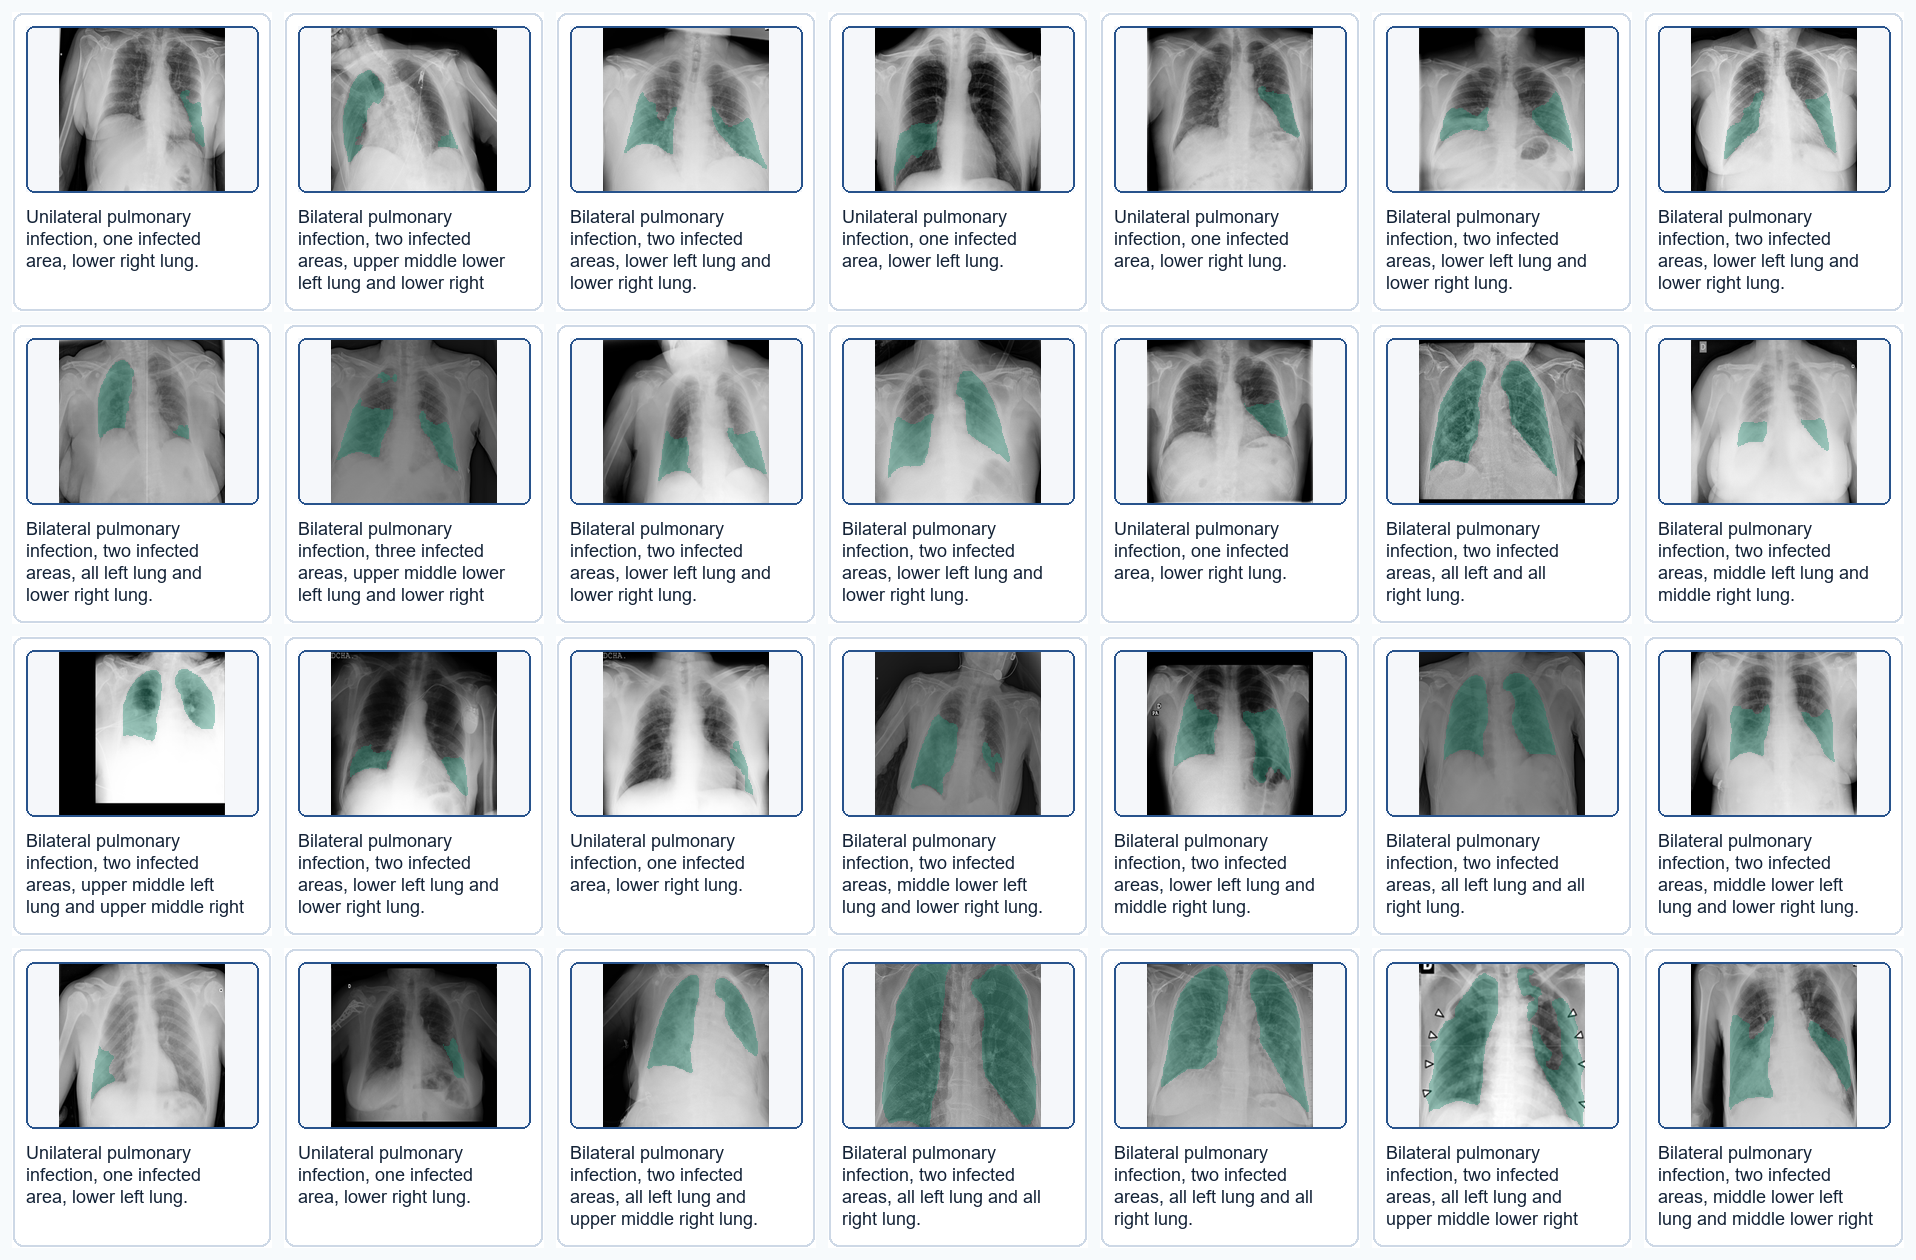
\includegraphics[width=0.96\textwidth]{figures/dataset_examples_qatacov19.png}
  \caption{Ví dụ ảnh, mask và văn bản chú thích của QaTa-COV19.}
  \label{fig:ch4-qata-examples}
\end{figure}

\textbf{EDA ảnh X-quang.} Ảnh trong QaTa-COV19 là ảnh X-quang ngực 2D, tức toàn bộ lồng ngực được chiếu lên một mặt phẳng. Đây là thuận lợi vì mô hình luôn nhìn thấy cấu trúc giải phẫu toàn cục như hai phổi, tim và cơ hoành; nhưng cũng là khó khăn vì xương sườn, mạch máu và mô mềm bị chồng lấp lên vùng tổn thương. Quan sát lưới mẫu cho thấy tổn thương COVID-19 thường không có biên sắc như vật thể tự nhiên; nhiều vùng chỉ là đám mờ cường độ thấp, lan dần ở đáy phổi hoặc vùng ngoại vi. Do đó, giả định ``biên rõ thì phân đoạn dễ'' không còn đúng. Mô hình cần vừa giữ chi tiết cục bộ của CNN, vừa dùng ngữ cảnh xa để nhận biết vùng mờ nằm trong cấu trúc phổi.

Từ EDA ảnh, có ba hệ quả cài đặt quan trọng. Thứ nhất, augmentation hình học phải tôn trọng giải phẫu. Xoay quá mạnh hoặc crop quá sát có thể làm mất quan hệ giữa mô tả ``left/right'', ``upper/lower'' và vị trí thật trên ảnh. Đặc biệt, lật ngang chỉ hợp lý nếu đồng thời hoán đổi thông tin trái/phải trong văn bản; nếu không, augmentation này tạo ra cặp ảnh--văn bản mâu thuẫn. Thứ hai, augmentation cường độ nên ở mức vừa phải vì ảnh X-quang có khác biệt độ sáng/độ tương phản giữa bệnh nhân và thiết bị, nhưng biến đổi quá mạnh có thể làm mất tín hiệu tổn thương mờ. Thứ ba, resize và chuẩn hóa cần giữ bố cục toàn phổi, bởi văn bản của QaTa-COV19 thường nói về vùng giải phẫu tương đối chứ không chỉ nói có/không có bệnh.

\textbf{EDA mask và ground truth.} Ground truth \(y\) là mask mức điểm ảnh biểu diễn vùng tổn thương COVID-19. Mask này vừa là đầu ra xác thực trong huấn luyện có giám sát, vừa là chuẩn để tính Dice/IoU. Khác với classification, một mask đúng phải trả lời câu hỏi ``tổn thương nằm ở đâu'' chứ không chỉ ``ảnh có bệnh hay không''. Các mask trong QaTa-COV19 có độ lớn rất khác nhau: có mẫu vùng tổn thương lan rộng hai phổi, nhưng cũng có mẫu chỉ gồm một cụm mờ nhỏ. Điều này tạo ra mất cân bằng foreground/background rất mạnh. Nếu mô hình dự đoán quá bảo thủ, Dice có thể giảm vì bỏ sót vùng mờ; nếu dự đoán quá rộng, IoU bị phạt nặng do false positive trên nền phổi. Vì vậy, báo cáo dùng đồng thời Dice và IoU thay vì chỉ dùng một metric.

Về mặt học bán giám sát, sự không đồng đều của mask làm pseudo-label trở thành con dao hai lưỡi. Ở mức 25\% nhãn, pseudo-label giúp mở rộng tín hiệu học, nhưng pseudo-label nhiễu ở vùng biên mờ có thể kéo mô hình về dự đoán sai. Đây là lý do EPI và LV loss cần được đọc như cơ chế kiểm soát chất lượng nhãn tạm: EPI làm mượt dự đoán qua nhiều vòng, còn LV loss dùng văn bản để ràng buộc nhãn giả không đi lệch ngữ nghĩa ảnh--văn bản.

\begin{figure}[H]
  \centering
  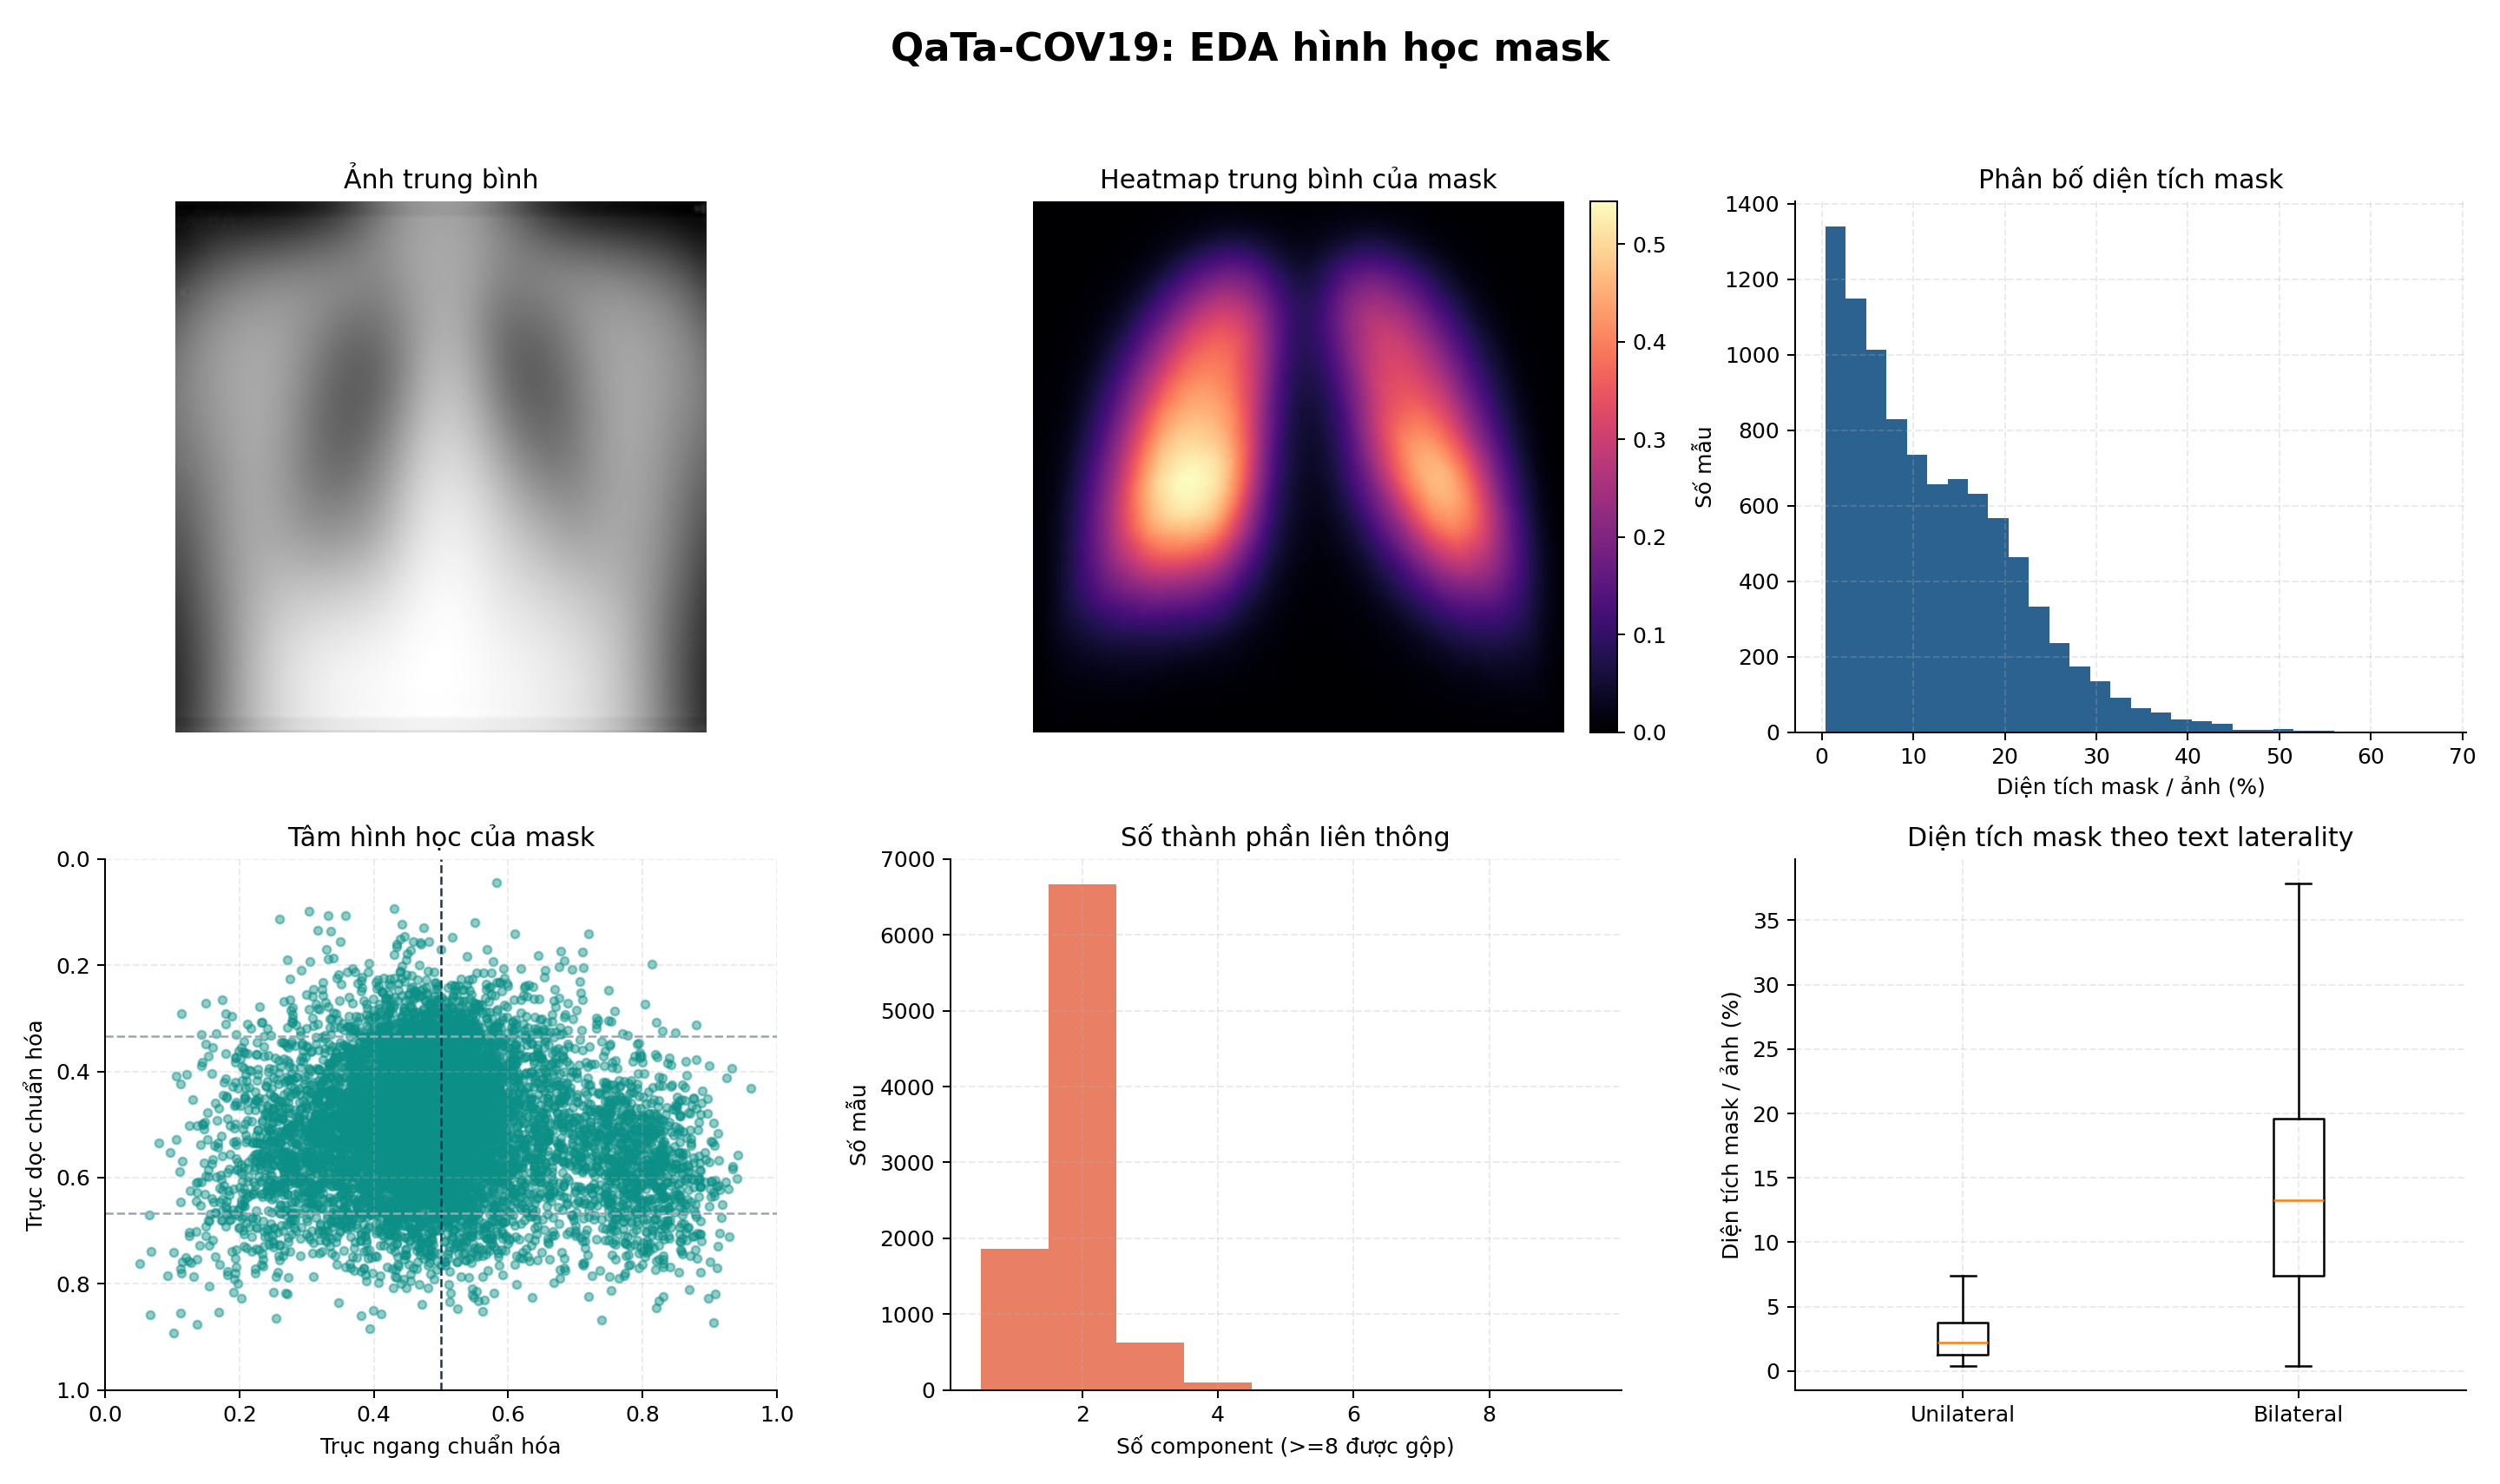
\includegraphics[width=0.96\textwidth]{figures/qata_mask_geometry_eda.png}
  \caption{EDA hình học mask của QaTa-COV19: phân bố diện tích foreground, ảnh trung bình, heatmap mask trung bình, tâm tổn thương và số thành phần liên thông.}
  \label{fig:ch4-qata-mask-geometry}
\end{figure}

Kết quả EDA hình học cho thấy toàn bộ 9258 mẫu QaTa-COV19 đều có mask khác rỗng. Diện tích tổn thương trung vị chiếm khoảng 10.15\% ảnh, trung bình 12.10\%, với tứ phân vị 25\%--75\% là 4.49\%--17.92\%. Chỉ khoảng 3.75\% mẫu có foreground nhỏ hơn 1\%, nên QaTa-COV19 không phải tập mà vật thể luôn cực nhỏ; khó khăn chính nằm ở biên mờ, độ lan không đều và sự chồng lấp giải phẫu trên X-quang. Số thành phần liên thông trung vị là 2; riêng 6667/9258 mẫu có đúng 2 thành phần, phù hợp với trực giác tổn thương hai phổi. Tâm mask trung bình gần giữa ảnh \((x \approx 0.497, y \approx 0.500)\), cho thấy bố cục hai phổi khá cân bằng. Từ đó, augmentation nên giữ toàn bộ cấu trúc lồng ngực và không được tùy tiện lật trái/phải nếu văn bản không được cập nhật tương ứng. Với pseudo-label, yêu cầu quan trọng không chỉ là dự đoán có foreground, mà còn phải giữ được cấu trúc hai bên và tránh gom các vùng mờ thành một blob sai hình thái.

\textbf{EDA văn bản chú thích.} văn bản chú thích của QaTa-COV19 là văn bản ngắn có cấu trúc, không phải toàn bộ bệnh án tự do. Trong 9258 mô tả, có 7338 mẫu hai bên và 1920 mẫu một bên; số vùng nhiễm thường gặp nhất là hai vùng với 6862 mẫu. Các cụm vị trí được lặp lại nhiều gồm phổi trái/phải, upper, middle, lower và all lung. Điều này cho thấy văn bản trong QaTa-COV19 giống một mô tả giải phẫu có quy tắc hơn là ngôn ngữ tự nhiên mở. Văn bản không thể thay thế mask vì nó không chứa biên mức điểm ảnh, nhưng nó chỉ ra ``nên chú ý vùng nào'' và ``tổn thương lan theo kiểu gì''.

\begin{figure}[H]
  \centering
  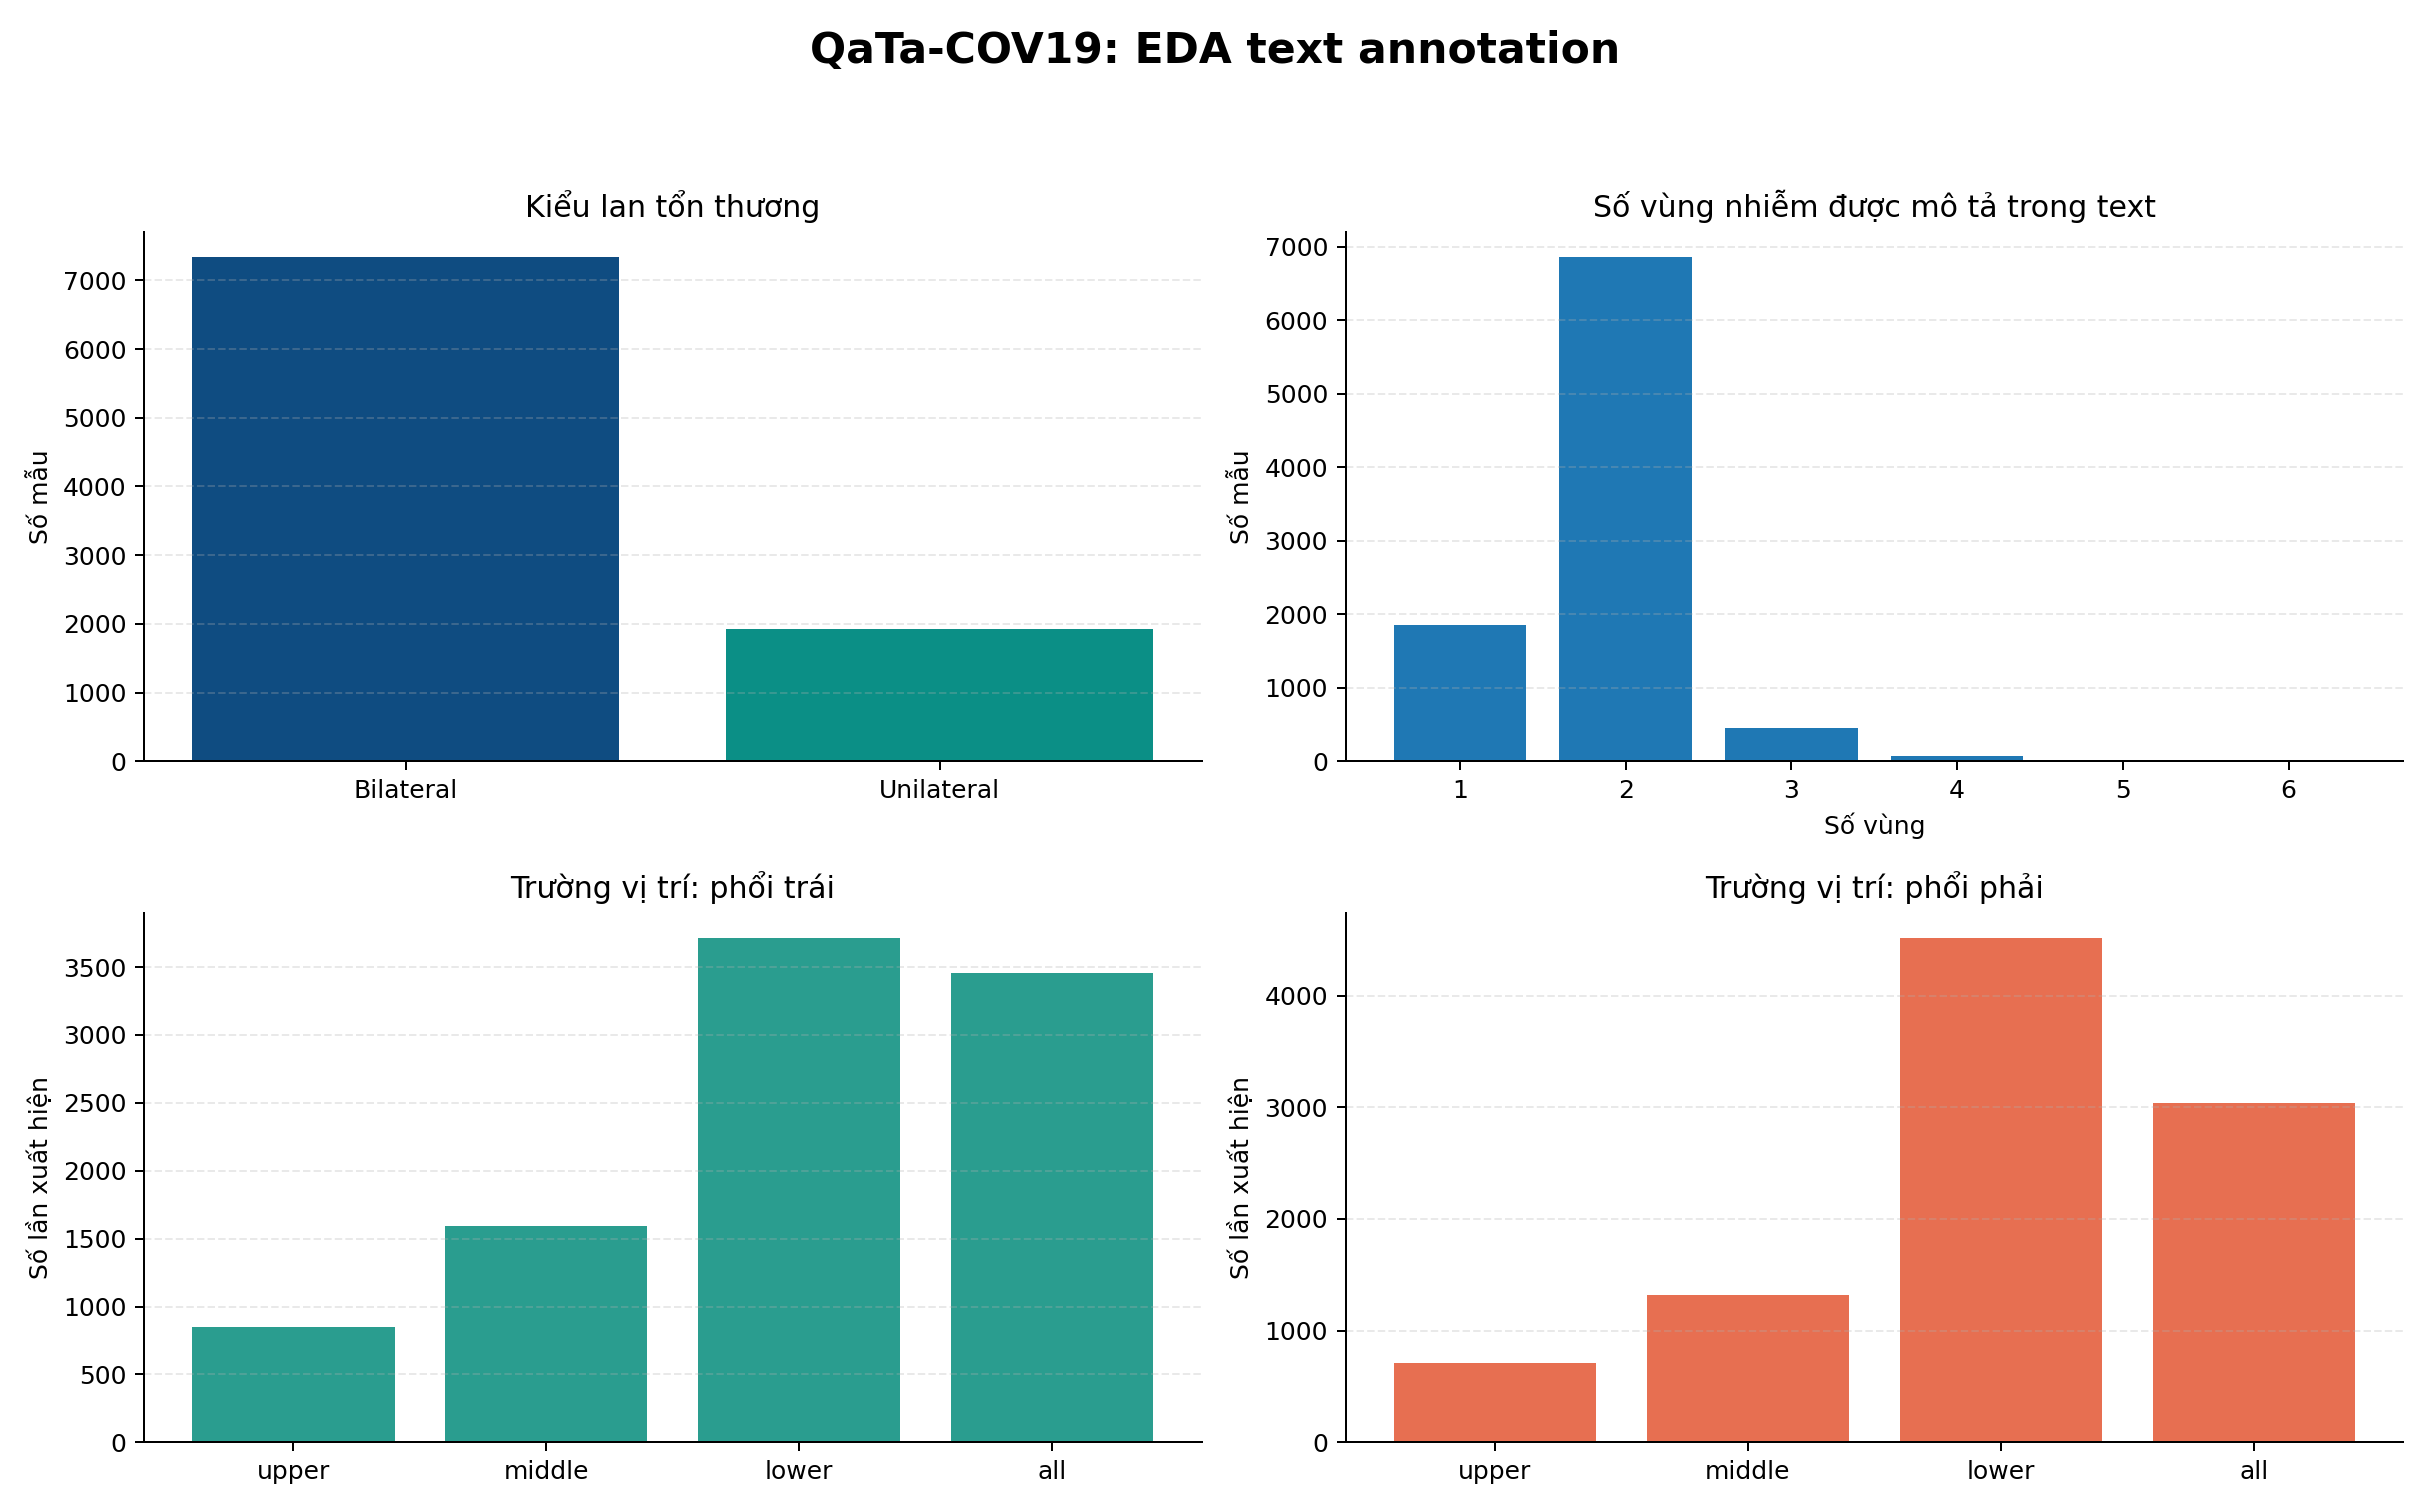
\includegraphics[width=0.96\textwidth]{figures/dataset_text_eda_qatacov19.png}
  \caption{EDA cấu trúc văn bản chú thích của QaTa-COV19.}
  \label{fig:ch4-qata-văn bản-eda}
\end{figure}

\begin{figure}[H]
  \centering
  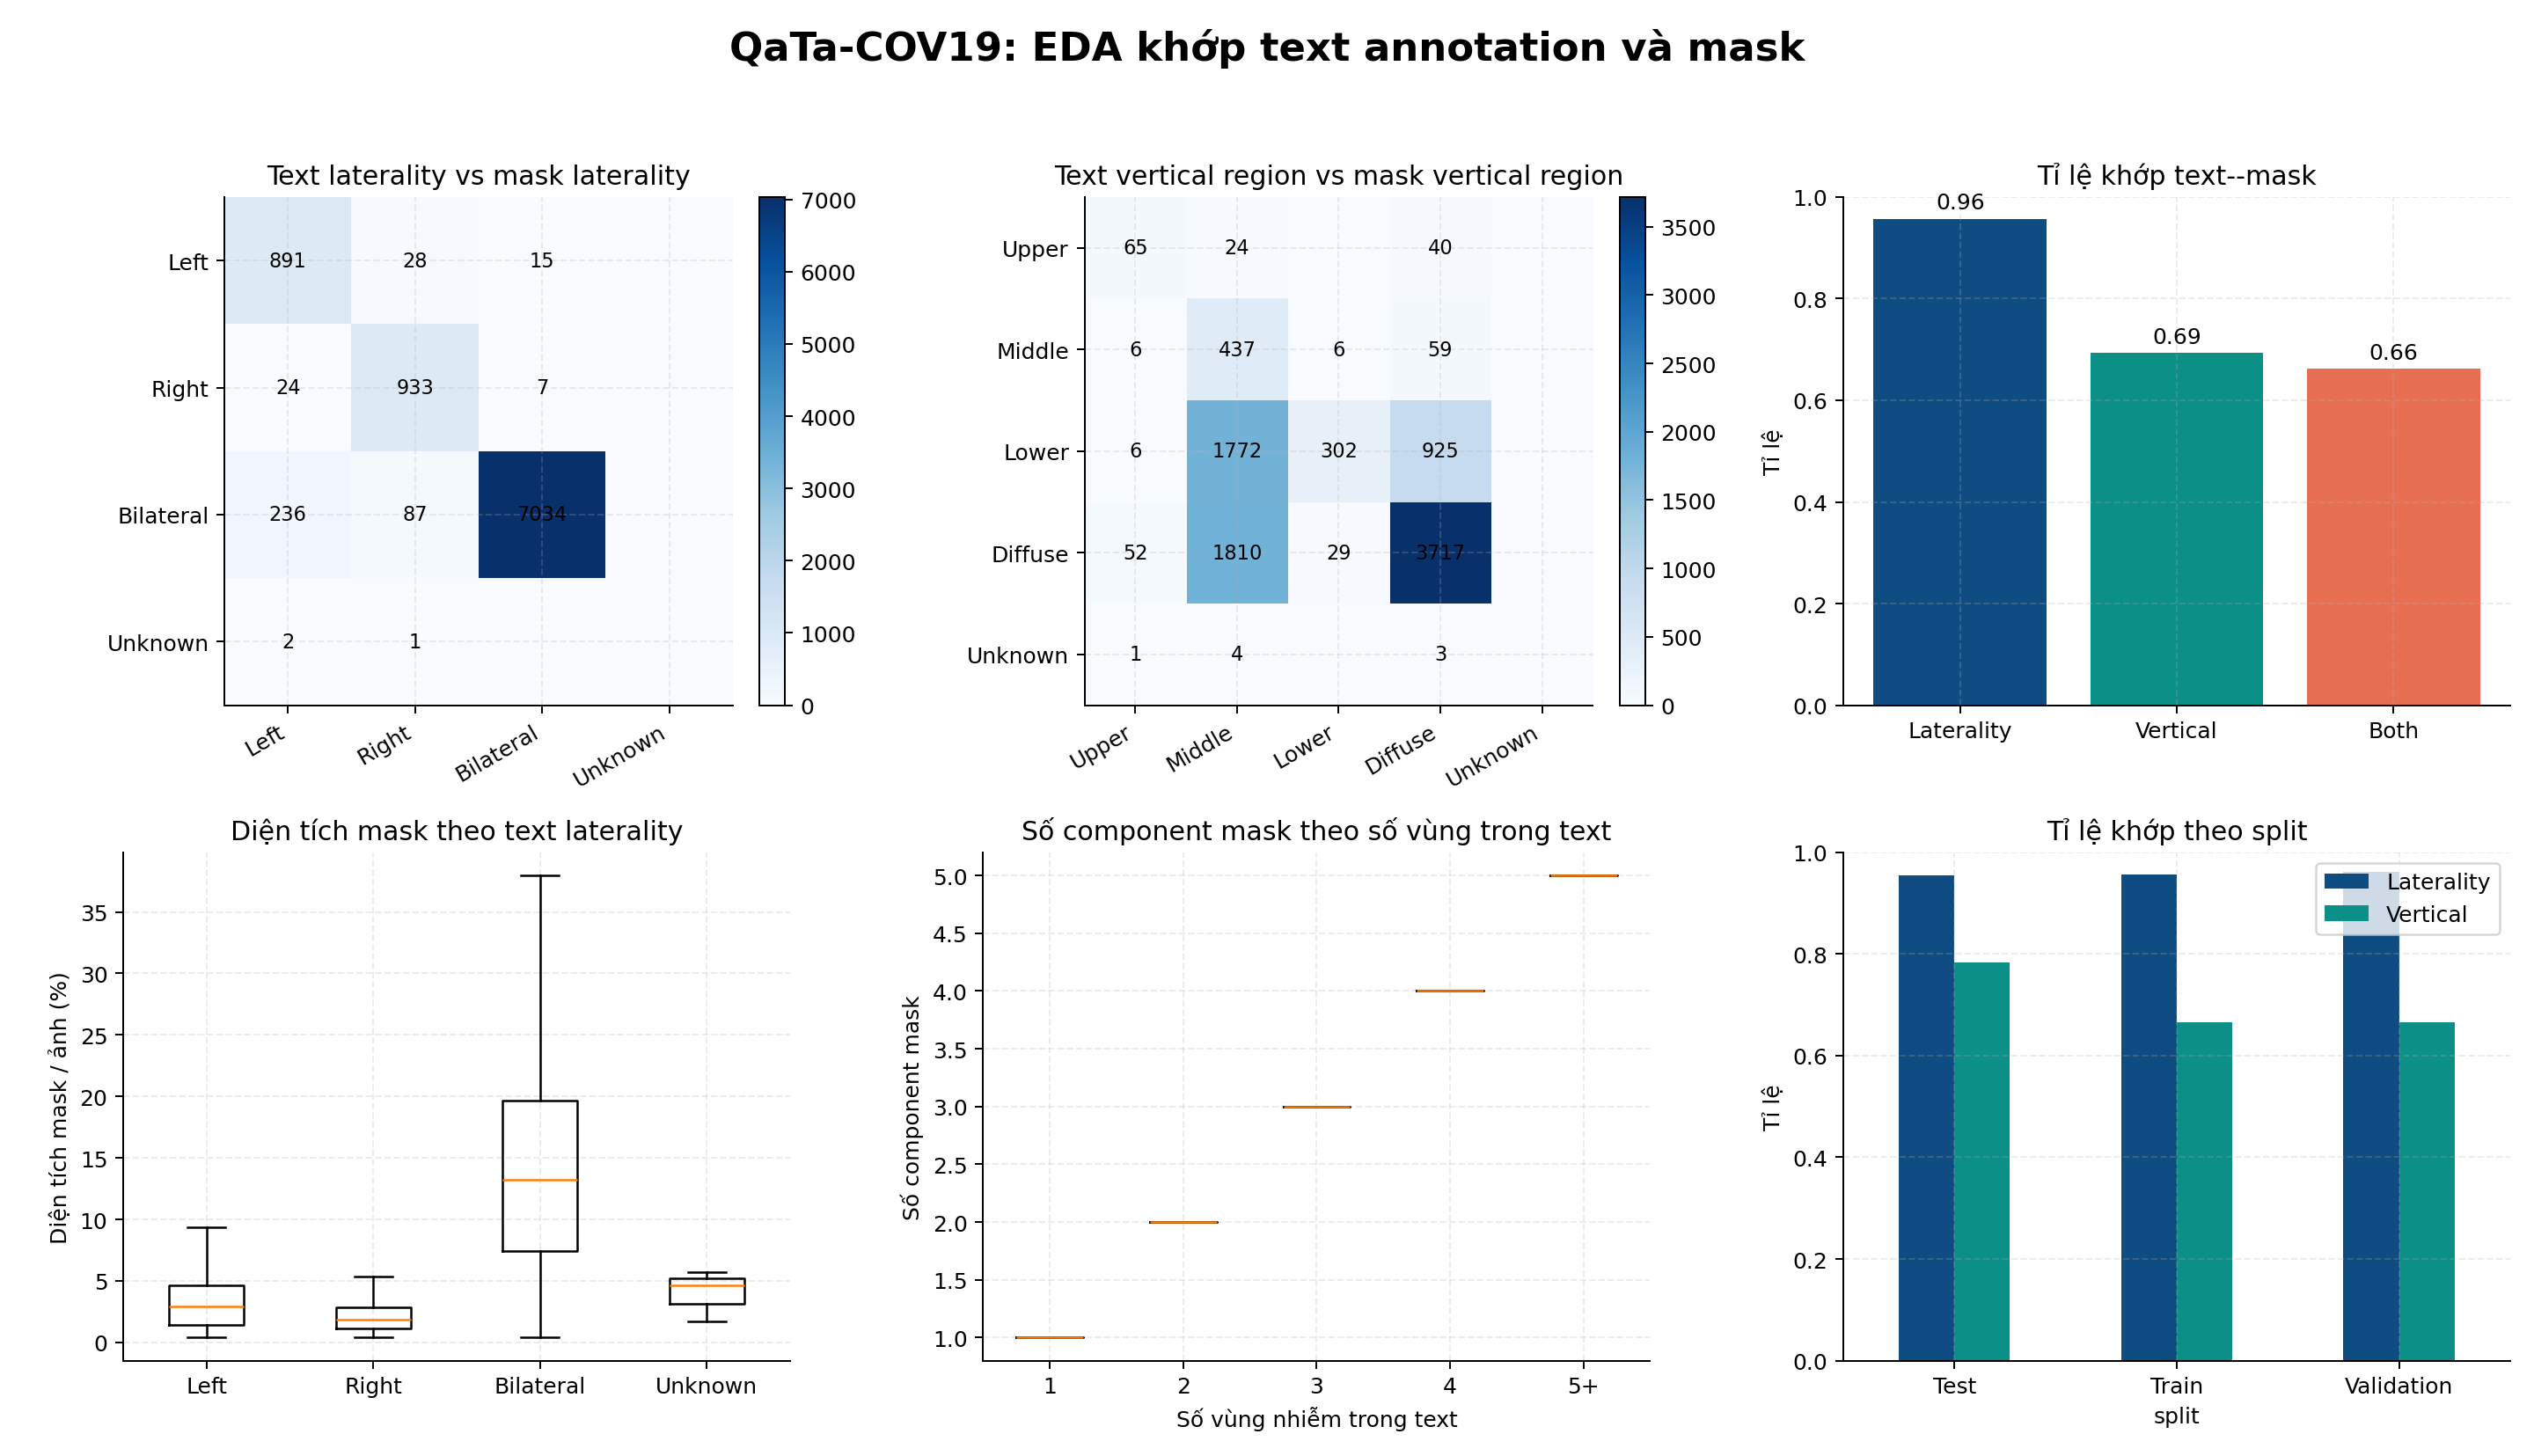
\includegraphics[width=0.96\textwidth]{figures/qata_text_mask_alignment.png}
  \caption{Đối sánh văn bản chú thích và mask của QaTa-COV19 theo trái/phải, tầng giải phẫu và số vùng nhiễm.}
  \label{fig:ch4-qata-văn bản-mask-alignment}
\end{figure}

Đối sánh văn bản--mask cho thấy văn bản của QaTa-COV19 có quan hệ hình học rõ với mask. Tỉ lệ khớp trái/phải đạt 95.68\%, nghĩa là khi văn bản nói tổn thương trái, phải hoặc hai bên, mask thường nằm đúng phía tương ứng. Tỉ lệ khớp tầng giải phẫu upper/middle/lower/diffuse thấp hơn, đạt 69.26\%, và tỉ lệ khớp đồng thời cả trái/phải lẫn tầng giải phẫu đạt 66.17\%. Điều này hợp lý vì ảnh X-quang là ảnh chiếu 2D: vùng lower trong mô tả lâm sàng có thể trải lên vùng giữa ảnh sau chiếu, hoặc tổn thương lan mờ khiến ranh giới tầng không sắc. Đáng chú ý, tương quan giữa số vùng nhiễm trong văn bản và số thành phần liên thông của mask đạt 0.911. Vì vậy, văn bản chú thích không phải phần trang trí; nó thật sự chứa tín hiệu vị trí, mức lan và số vùng tổn thương. Tuy nhiên, vì văn bản không mô tả biên điểm ảnh, nó nên được dùng như prior ngữ nghĩa trong LV Fusion/LV loss, không được xem như ground truth thay thế mask.

\textbf{Insight từ bộ mã hóa văn bản.} Một insight quan trọng từ LViT là văn bản y khoa trong bài toán này không nhất thiết cần một language bộ mã hóa quá sâu để có ích cho phân đoạn. LViT khai thác biểu diễn ở mức embedding và đưa ngữ nghĩa vào đặc trưng ảnh qua LV Fusion, thay vì biến bài toán thành hiểu bệnh án dài. Kết quả này phù hợp với EDA của QaTa-COV19: văn bản chú thích có ngữ pháp khá cố định, nhiều token vị trí lặp lại và ít câu văn tự do; đồng thời các thống kê đối sánh cho thấy trái/phải và số vùng nhiễm có tương quan mạnh với mask thật. Vì vậy, giả thuyết hợp lý là chất lượng chuẩn hóa prompt và cách đưa embedding vào ảnh có thể quan trọng không kém, thậm chí quan trọng hơn, việc dùng một bộ mã hóa ngôn ngữ ngày càng nặng. Đây là cơ sở để phần sau thử prompt normalization, BiomedBERT và cấu hình NoBERT/BiGRU: không phủ nhận vai trò của văn bản, mà kiểm tra văn bản cần được mã hóa sâu đến mức nào trong một tập văn bản có cấu trúc mạnh.

\textbf{Insight dẫn sang thiết kế thử nghiệm.} Từ các quan sát trên, QaTa-COV19 được dùng để kiểm tra bốn nhóm quyết định. Nhóm thứ nhất là tỉ lệ nhãn 25\%, 50\%, 100\%, nhằm xem cải tiến còn hữu ích khi lượng mask thật thay đổi. Nhóm thứ hai là chuẩn hóa prompt, vì các mô tả cùng nghĩa có thể khác hình thức và cần được đưa về biểu diễn ổn định hơn. Nhóm thứ ba là ablation bộ mã hóa văn bản, nhằm kiểm tra liệu embedding có cấu trúc thấp hơn có đủ cạnh tranh với bộ mã hóa y sinh mạnh hơn hay không. Nhóm thứ tư là pseudo-label/EPI/LV loss, vì vùng tổn thương mờ và thiếu nhãn khiến nhãn giả phải được kiểm soát thay vì dùng trực tiếp.

\subsection{MosMedData+}

\textbf{Tổng quan và nguồn dữ liệu.} MosMedData+ là bộ CT ngực COVID-19 được dùng trong LViT để đánh giá trên miền ảnh CT \cite{morozov2020mosmeddata,hofmanninger2020automatic}. Tập này gồm 2183 mẫu train, 273 mẫu validation và 273 mẫu test. Khác với QaTa-COV19, mỗi mẫu là một lát CT thay vì ảnh chiếu X-quang. MosMedData+ được xây dựng từ nhiều nguồn, bao gồm nhóm dữ liệu MosMedData, Coronacases--Radiopaedia và MedSeg CT. Vì vậy, đây không chỉ là một tập CT đơn thuần, mà là một bài kiểm tra chuyển miền: mô hình phải xử lý sự khác nhau về nguồn ảnh, trường nhìn, cường độ và kiểu tổn thương.

\begin{figure}[H]
  \centering
  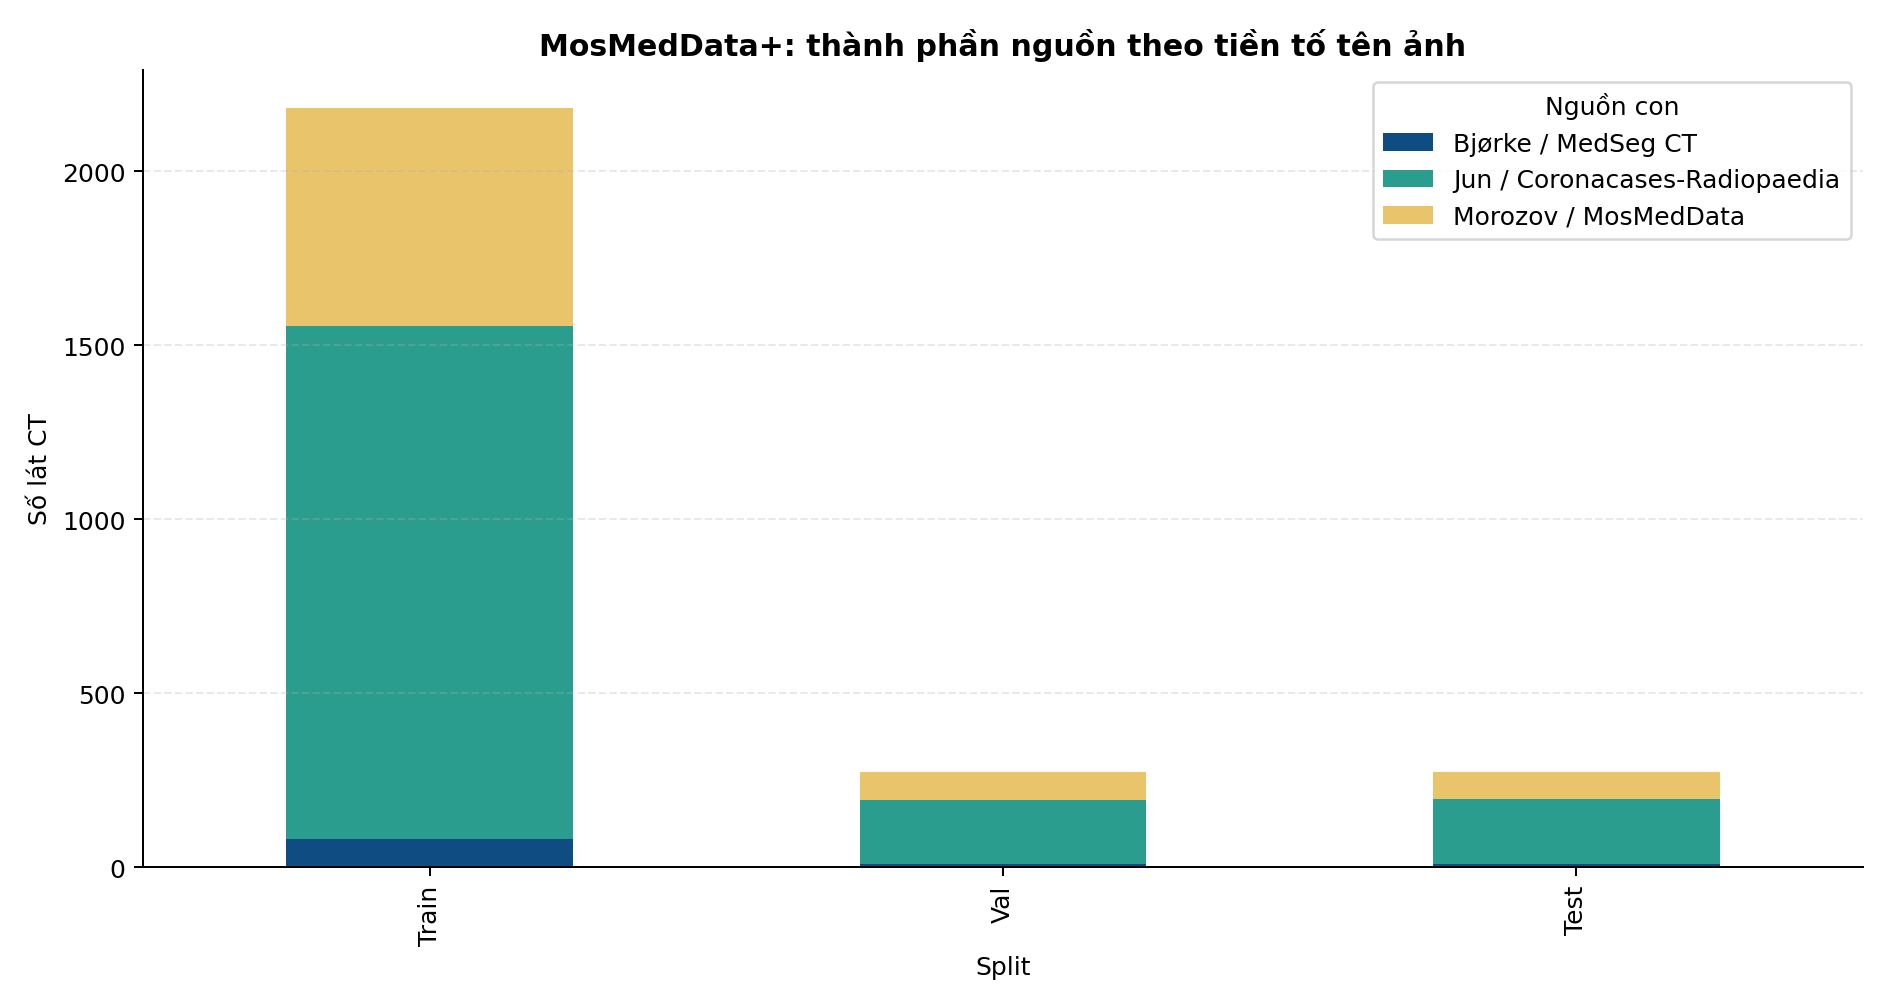
\includegraphics[width=0.96\textwidth]{figures/dataset_sources_mosmeddata.png}
  \caption{Thành phần nguồn dữ liệu trong MosMedData+.}
  \label{fig:ch4-mosmed-sources}
\end{figure}

\begin{figure}[H]
  \centering
  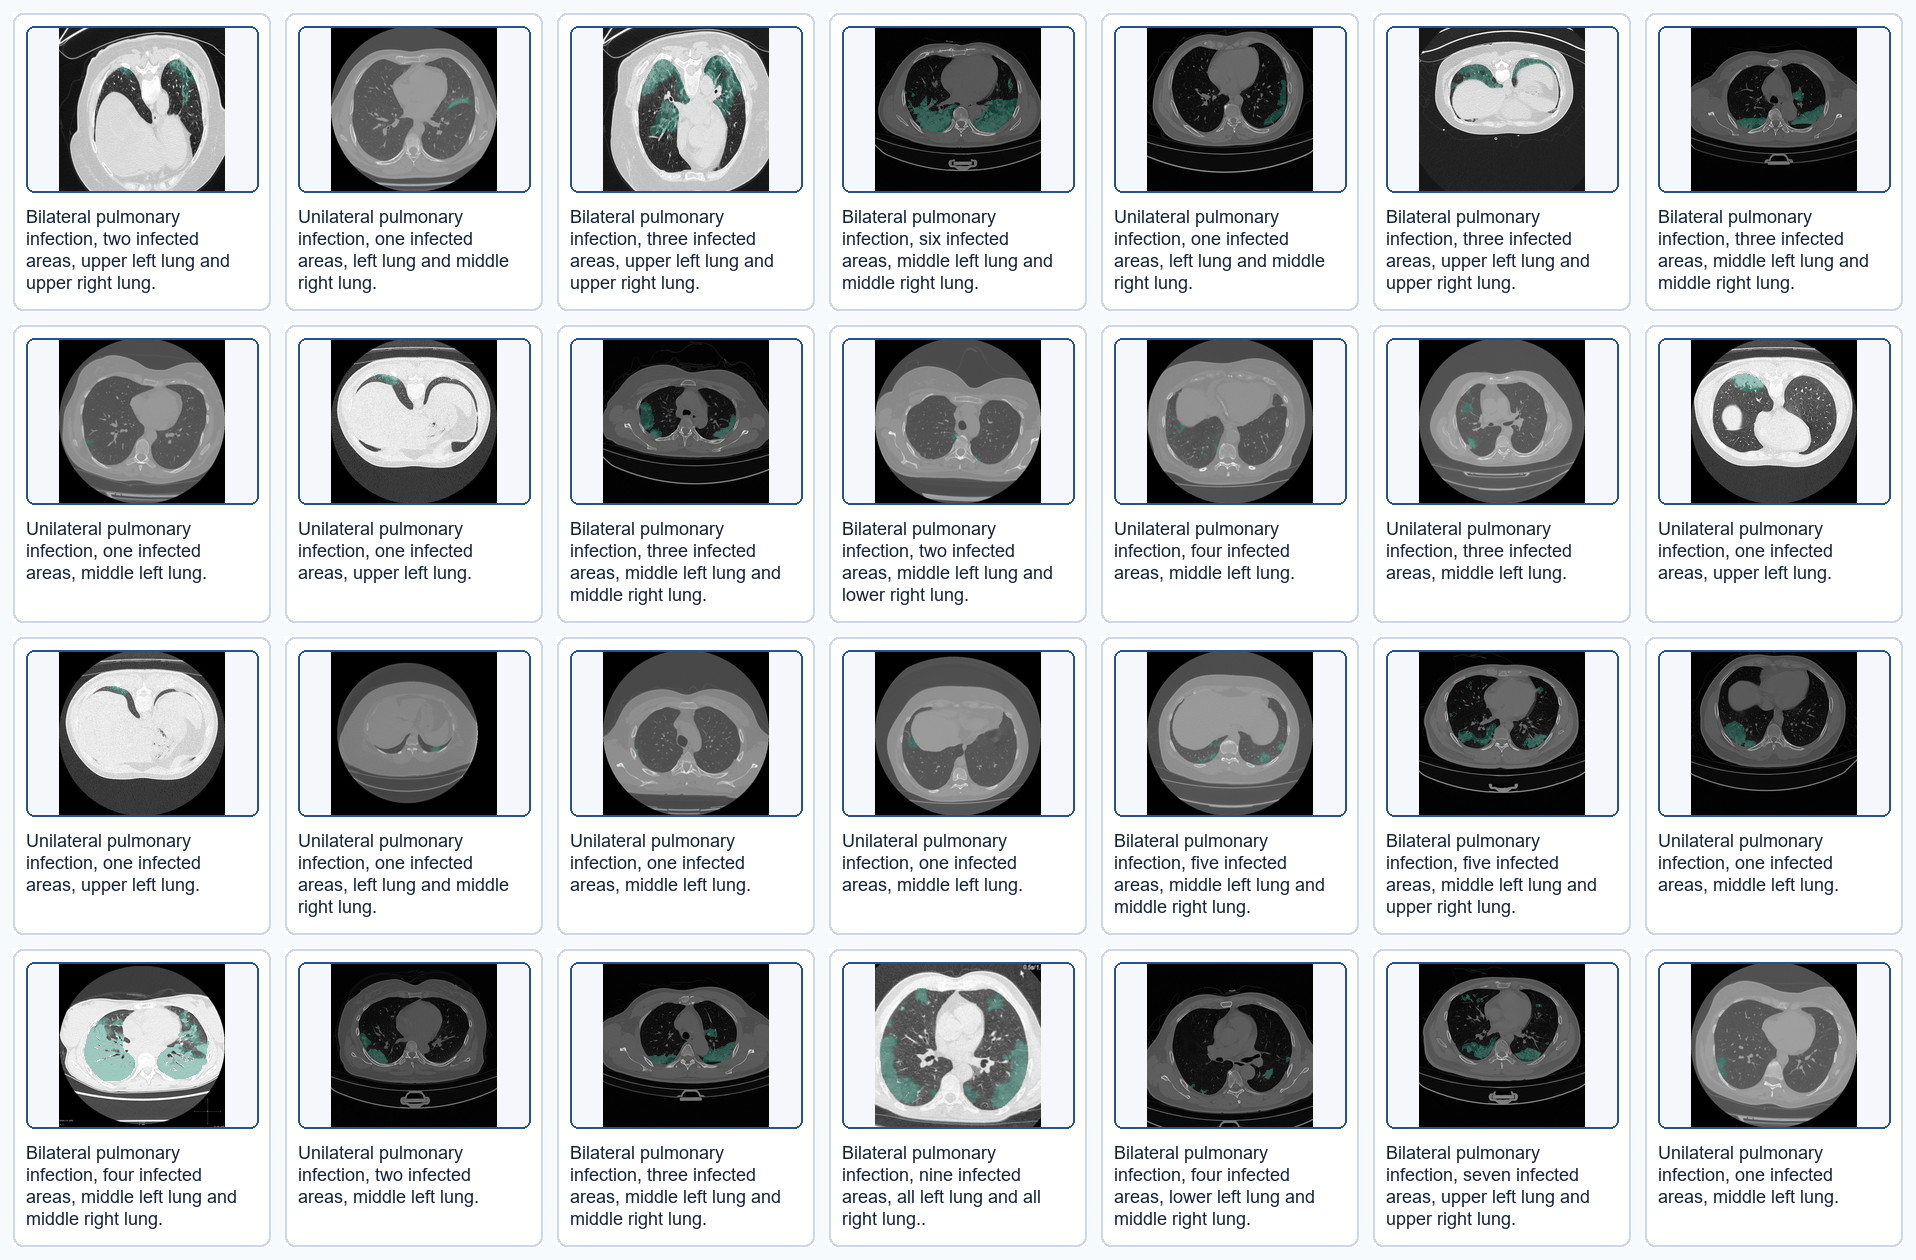
\includegraphics[width=0.96\textwidth]{figures/dataset_examples_mosmeddata.png}
  \caption{Ví dụ ảnh, mask và văn bản chú thích của MosMedData+.}
  \label{fig:ch4-mosmed-examples}
\end{figure}

\textbf{EDA ảnh CT.} CT có cường độ giàu thông tin hơn X-quang, nhưng mỗi lát chỉ là một mặt cắt của thể tích 3D. Vì vậy, một lát có thể chứa tổn thương rất rõ, rất nhỏ, rải rác, hoặc gần như không biểu hiện nhiều dù ca bệnh có tổn thương ở lát khác. Bối cảnh này làm bài toán khó theo cách khác với QaTa-COV19. Trên X-quang, mô hình học bố cục toàn lồng ngực; trên CT, mô hình phải nhạy với vị trí lát, hình dạng phổi trên lát đó và vùng tổn thương có thể nằm sát biên phổi. Ngoài ra, dữ liệu từ nhiều nguồn khiến nền ảnh, kích thước vùng phổi và mức tương phản không đồng nhất.

Từ EDA ảnh CT, các quyết định tiền xử lý trở nên quan trọng hơn so với QaTa-COV19. Crop vùng phổi giúp giảm nền ngoài cơ thể và buộc mô hình tập trung vào vùng có khả năng xuất hiện tổn thương. Tuy nhiên, crop quá mạnh có thể cắt mất tổn thương sát màng phổi, nên crop cần giữ biên phổi đủ rộng. Augmentation cũng cần nhẹ và có kiểm soát: biến đổi cường độ giúp mô hình bền hơn với khác biệt nguồn ảnh, nhưng biến dạng hình học quá mạnh có thể làm sai hình thái lát CT. Đây là lý do phần thực nghiệm trên MosMedData+ không chỉ so sánh bộ mã hóa văn bản, mà còn tách riêng tác động của crop, loss cleanup và LightAU.

\textbf{EDA mask và ground truth.} Ground truth \(y\) của MosMedData+ là mask mức điểm ảnh vùng nhiễm trùng trên lát CT. So với X-quang, biên tổn thương trên CT có thể rõ hơn trong một số lát, nhưng foreground thường nhỏ, phân mảnh và thay đổi mạnh giữa các lát. Điều này làm Dice/IoU nhạy với threshold sau sigmoid. Nếu threshold quá cao, mô hình bỏ sót các vùng tổn thương mờ; nếu threshold quá thấp, mô hình tạo nhiều false positive quanh biên phổi. Vì vậy, MosMedData+ phù hợp để kiểm tra không chỉ khả năng học đặc trưng, mà còn độ ổn định của hậu xử lý dự đoán xác suất thành mask nhị phân.

Một điểm cần nhấn mạnh là mask CT mang tính lát cắt. văn bản chú thích có thể mô tả tình trạng hoặc vùng tổn thương của ca bệnh, nhưng mask chỉ xác nhận vùng tổn thương trên lát hiện tại. Do đó, sự khớp giữa văn bản và mask trên MosMedData+ có thể yếu hơn QaTa-COV19. Trong trường hợp này, văn bản vẫn hữu ích như tín hiệu ngữ nghĩa, nhưng không nên để văn bản áp đảo bằng chứng ảnh. Đây là lý do các thử nghiệm về pseudo-label trên MosMedData+ cần được đọc cùng với crop, threshold và loss: nhãn giả tốt phải vừa ổn định theo ảnh, vừa không mâu thuẫn với văn bản.

\begin{figure}[H]
  \centering
  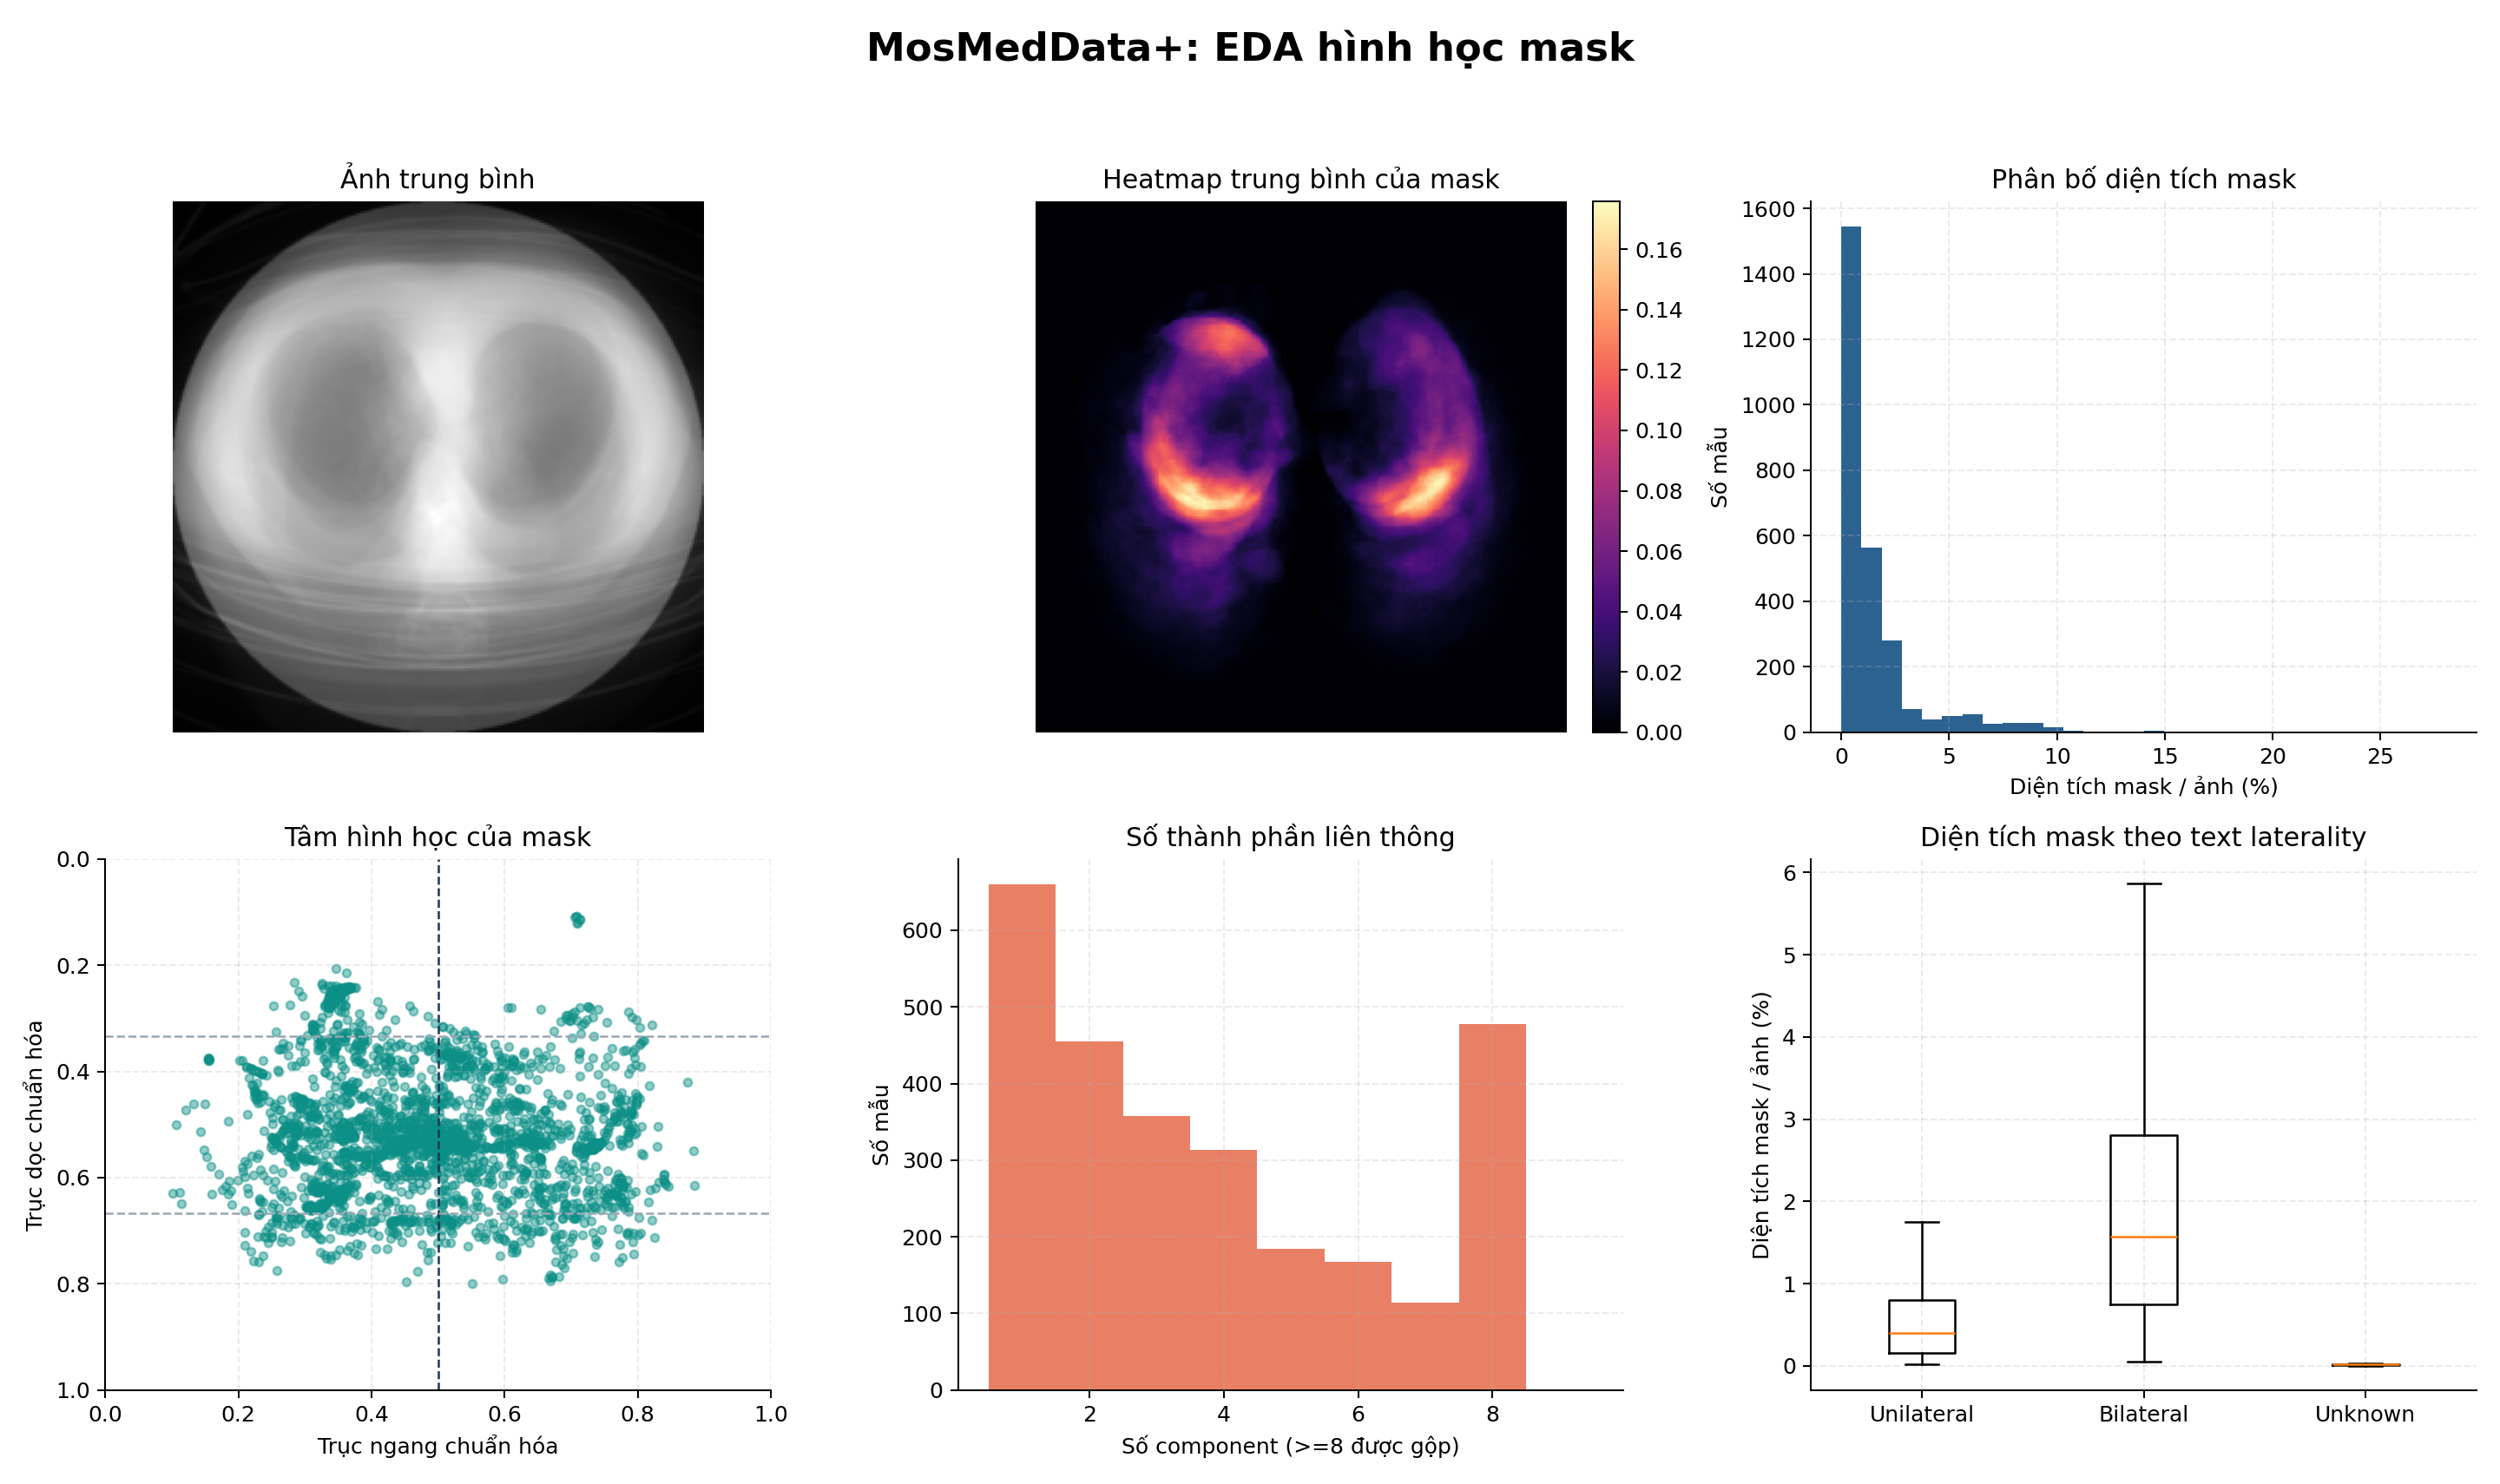
\includegraphics[width=0.96\textwidth]{figures/mosmed_mask_geometry_eda.png}
  \caption{EDA hình học mask của MosMedData+: phân bố diện tích foreground, ảnh trung bình, heatmap mask trung bình, tâm tổn thương và số thành phần liên thông.}
  \label{fig:ch4-mosmed-mask-geometry}
\end{figure}

Các thống kê hình học làm rõ vì sao MosMedData+ khó hơn theo hướng khác với QaTa-COV19. Trong 2729 mẫu, có 2728 mask khác rỗng và 1 mask rỗng. Diện tích tổn thương trung vị chỉ chiếm 0.758\% ảnh, trung bình 1.54\%; tứ phân vị 25\%--75\% là 0.302\%--1.674\%, và 58.54\% mẫu có foreground nhỏ hơn 1\%. Như vậy, phần lớn bài toán MosMedData+ là phân đoạn vùng rất nhỏ trên lát CT. Số thành phần liên thông trung vị là 3, tứ phân vị 75\% là 6 và phân vị 95\% lên tới 17, cho thấy mask không chỉ nhỏ mà còn rất phân mảnh. Đây là lý do MosMedData+ đặc biệt nhạy với threshold, loss và crop: một thay đổi nhỏ ở bản đồ xác suất có thể làm mất một cụm tổn thương, hoặc sinh thêm nhiều cụm giả quanh biên phổi. Insight này trực tiếp dẫn đến các thử nghiệm crop-only, loss cleanup, LightAU và so sánh threshold cố định với threshold chọn theo validation.

\textbf{EDA văn bản chú thích.} văn bản chú thích của MosMedData+ cũng được tổ chức theo tinh thần LViT, nhưng phân bố phức tạp hơn QaTa-COV19. Trong 2729 mô tả, số mẫu hai bên và một bên gần cân bằng: 1342 hai bên, 1340 một bên, và 47 mẫu khó quy về hai nhóm rõ ràng. Số vùng nhiễm trải rộng từ một đến chín vùng, thay vì tập trung mạnh ở hai vùng như QaTa-COV19. Các vị trí middle ở phổi trái/phải xuất hiện nhiều, trong khi all lung ít hơn. Phân bố này cho thấy MosMedData+ có đa dạng vị trí và mức độ lan tổn thương cao hơn, làm văn bản ít ``dễ đoán'' hơn.

\begin{figure}[H]
  \centering
  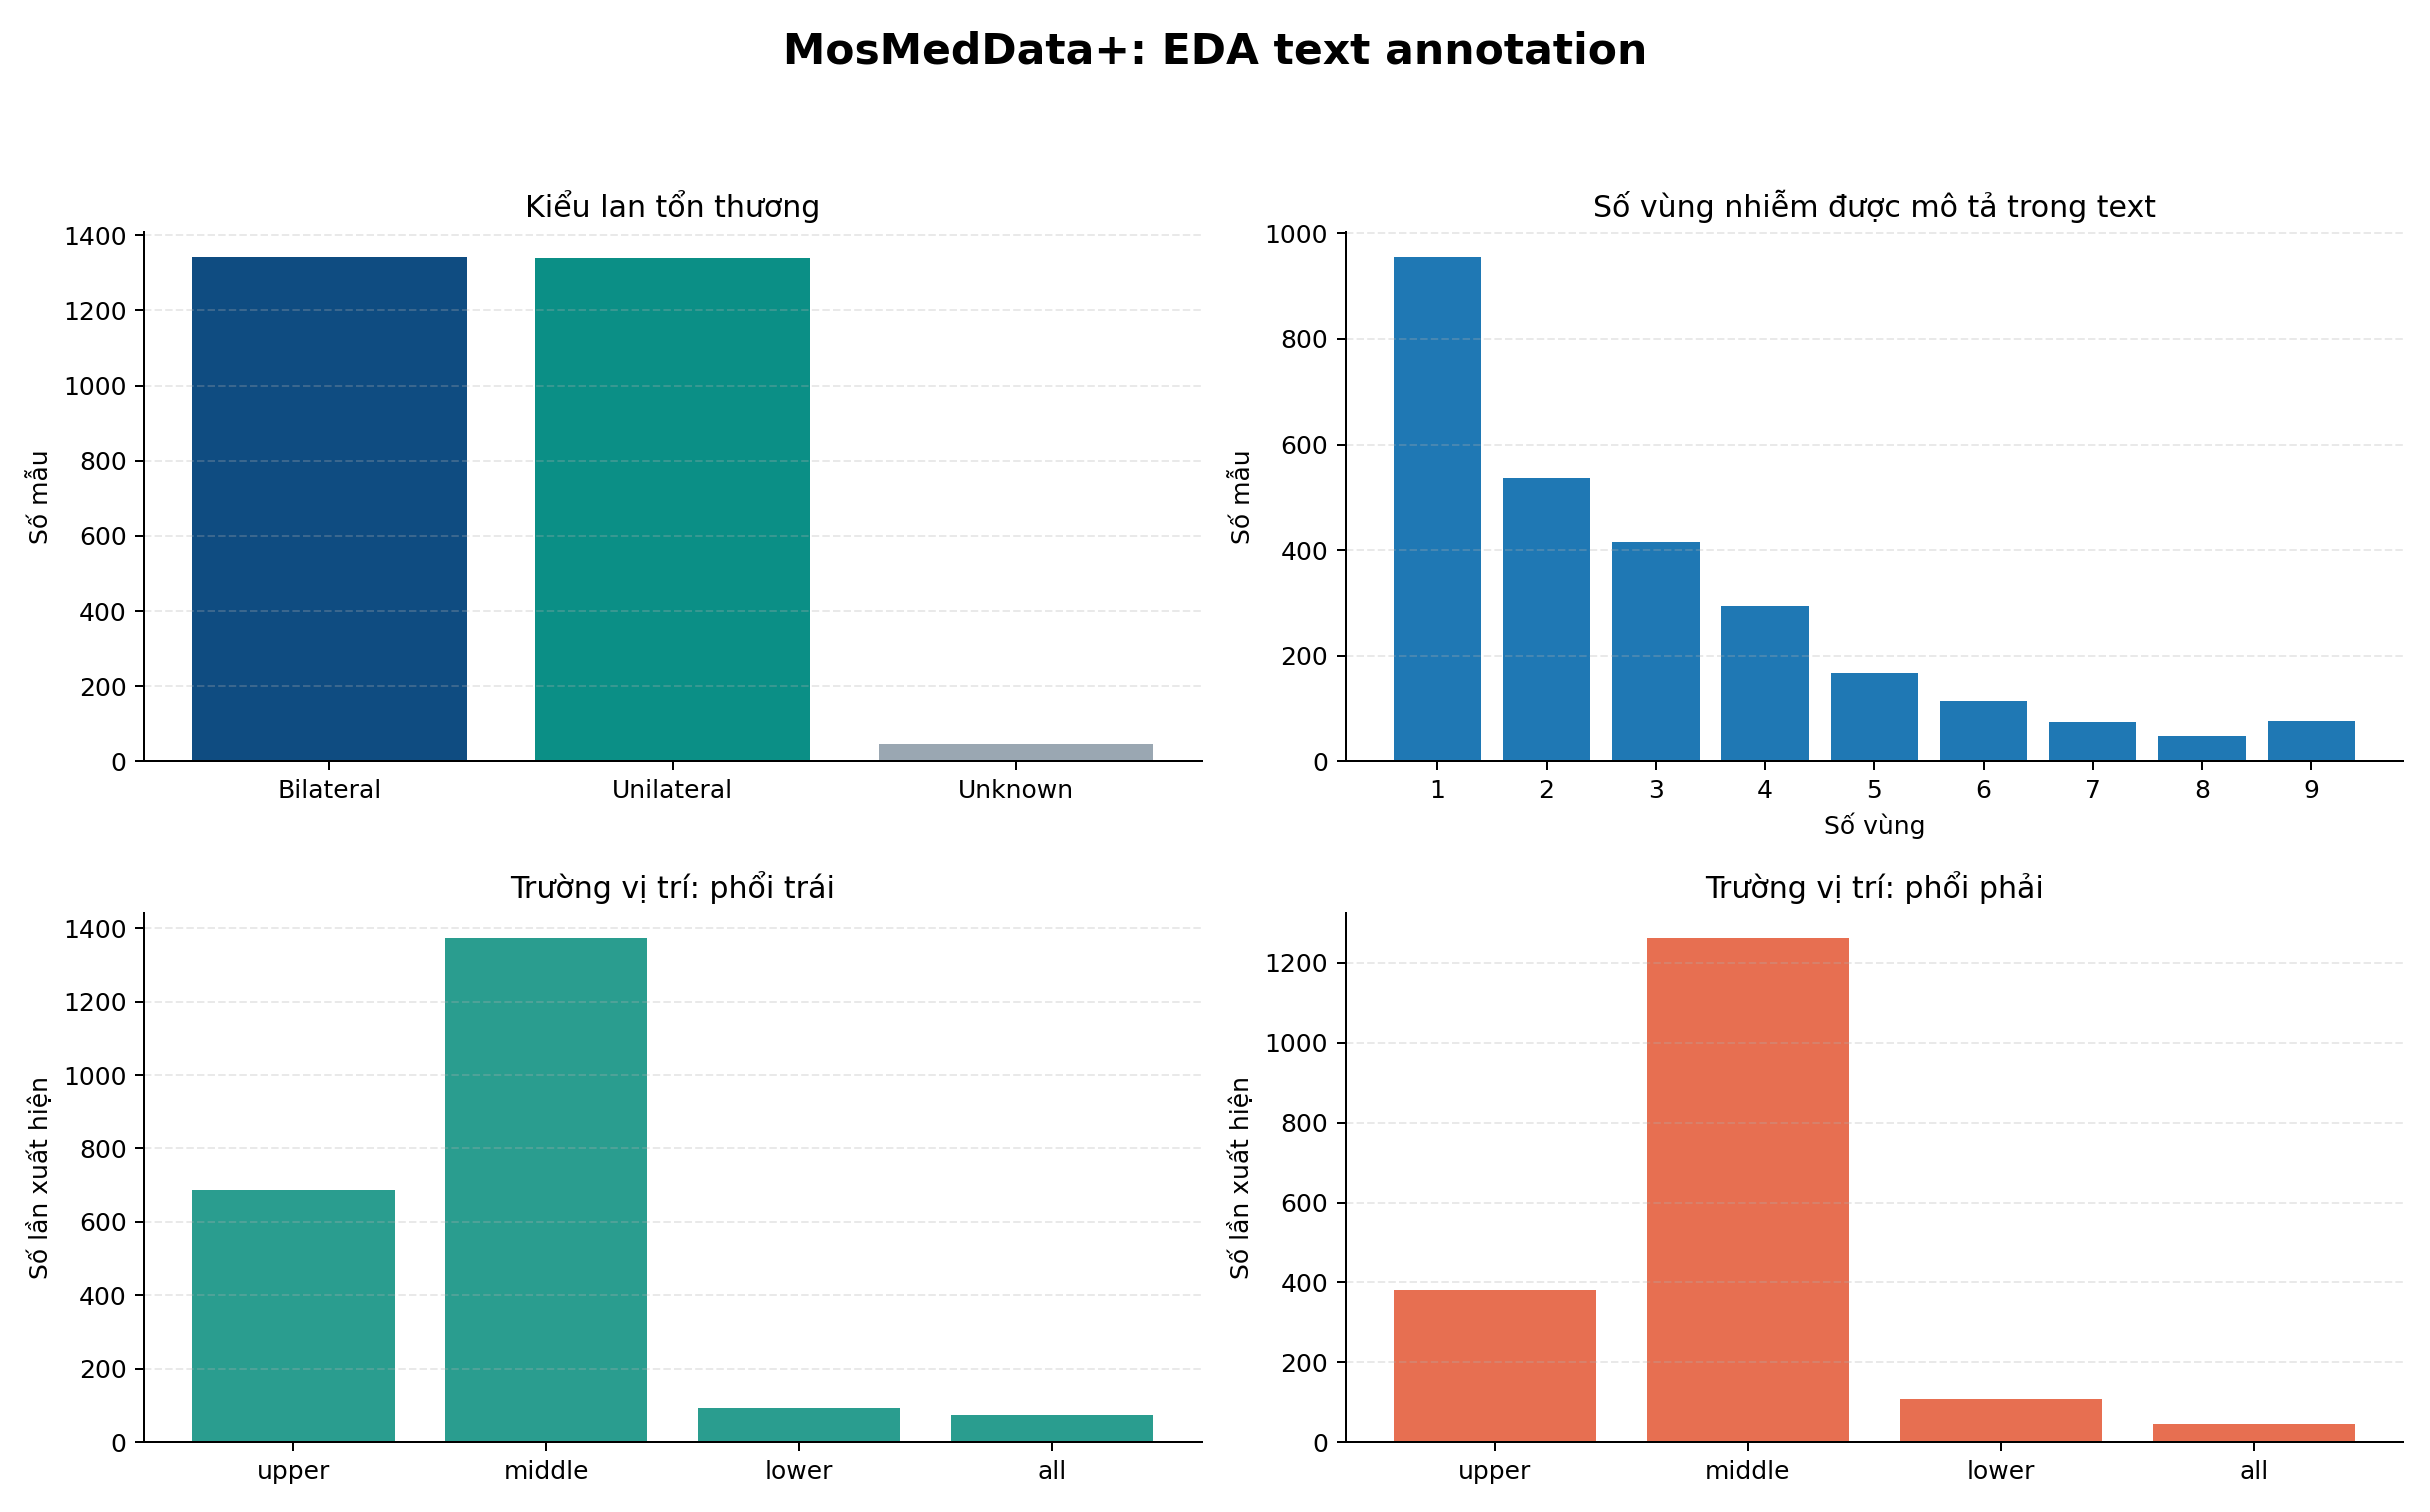
\includegraphics[width=0.96\textwidth]{figures/dataset_text_eda_mosmeddata.png}
  \caption{EDA cấu trúc văn bản chú thích của MosMedData+.}
  \label{fig:ch4-mosmed-văn bản-eda}
\end{figure}

\begin{figure}[H]
  \centering
  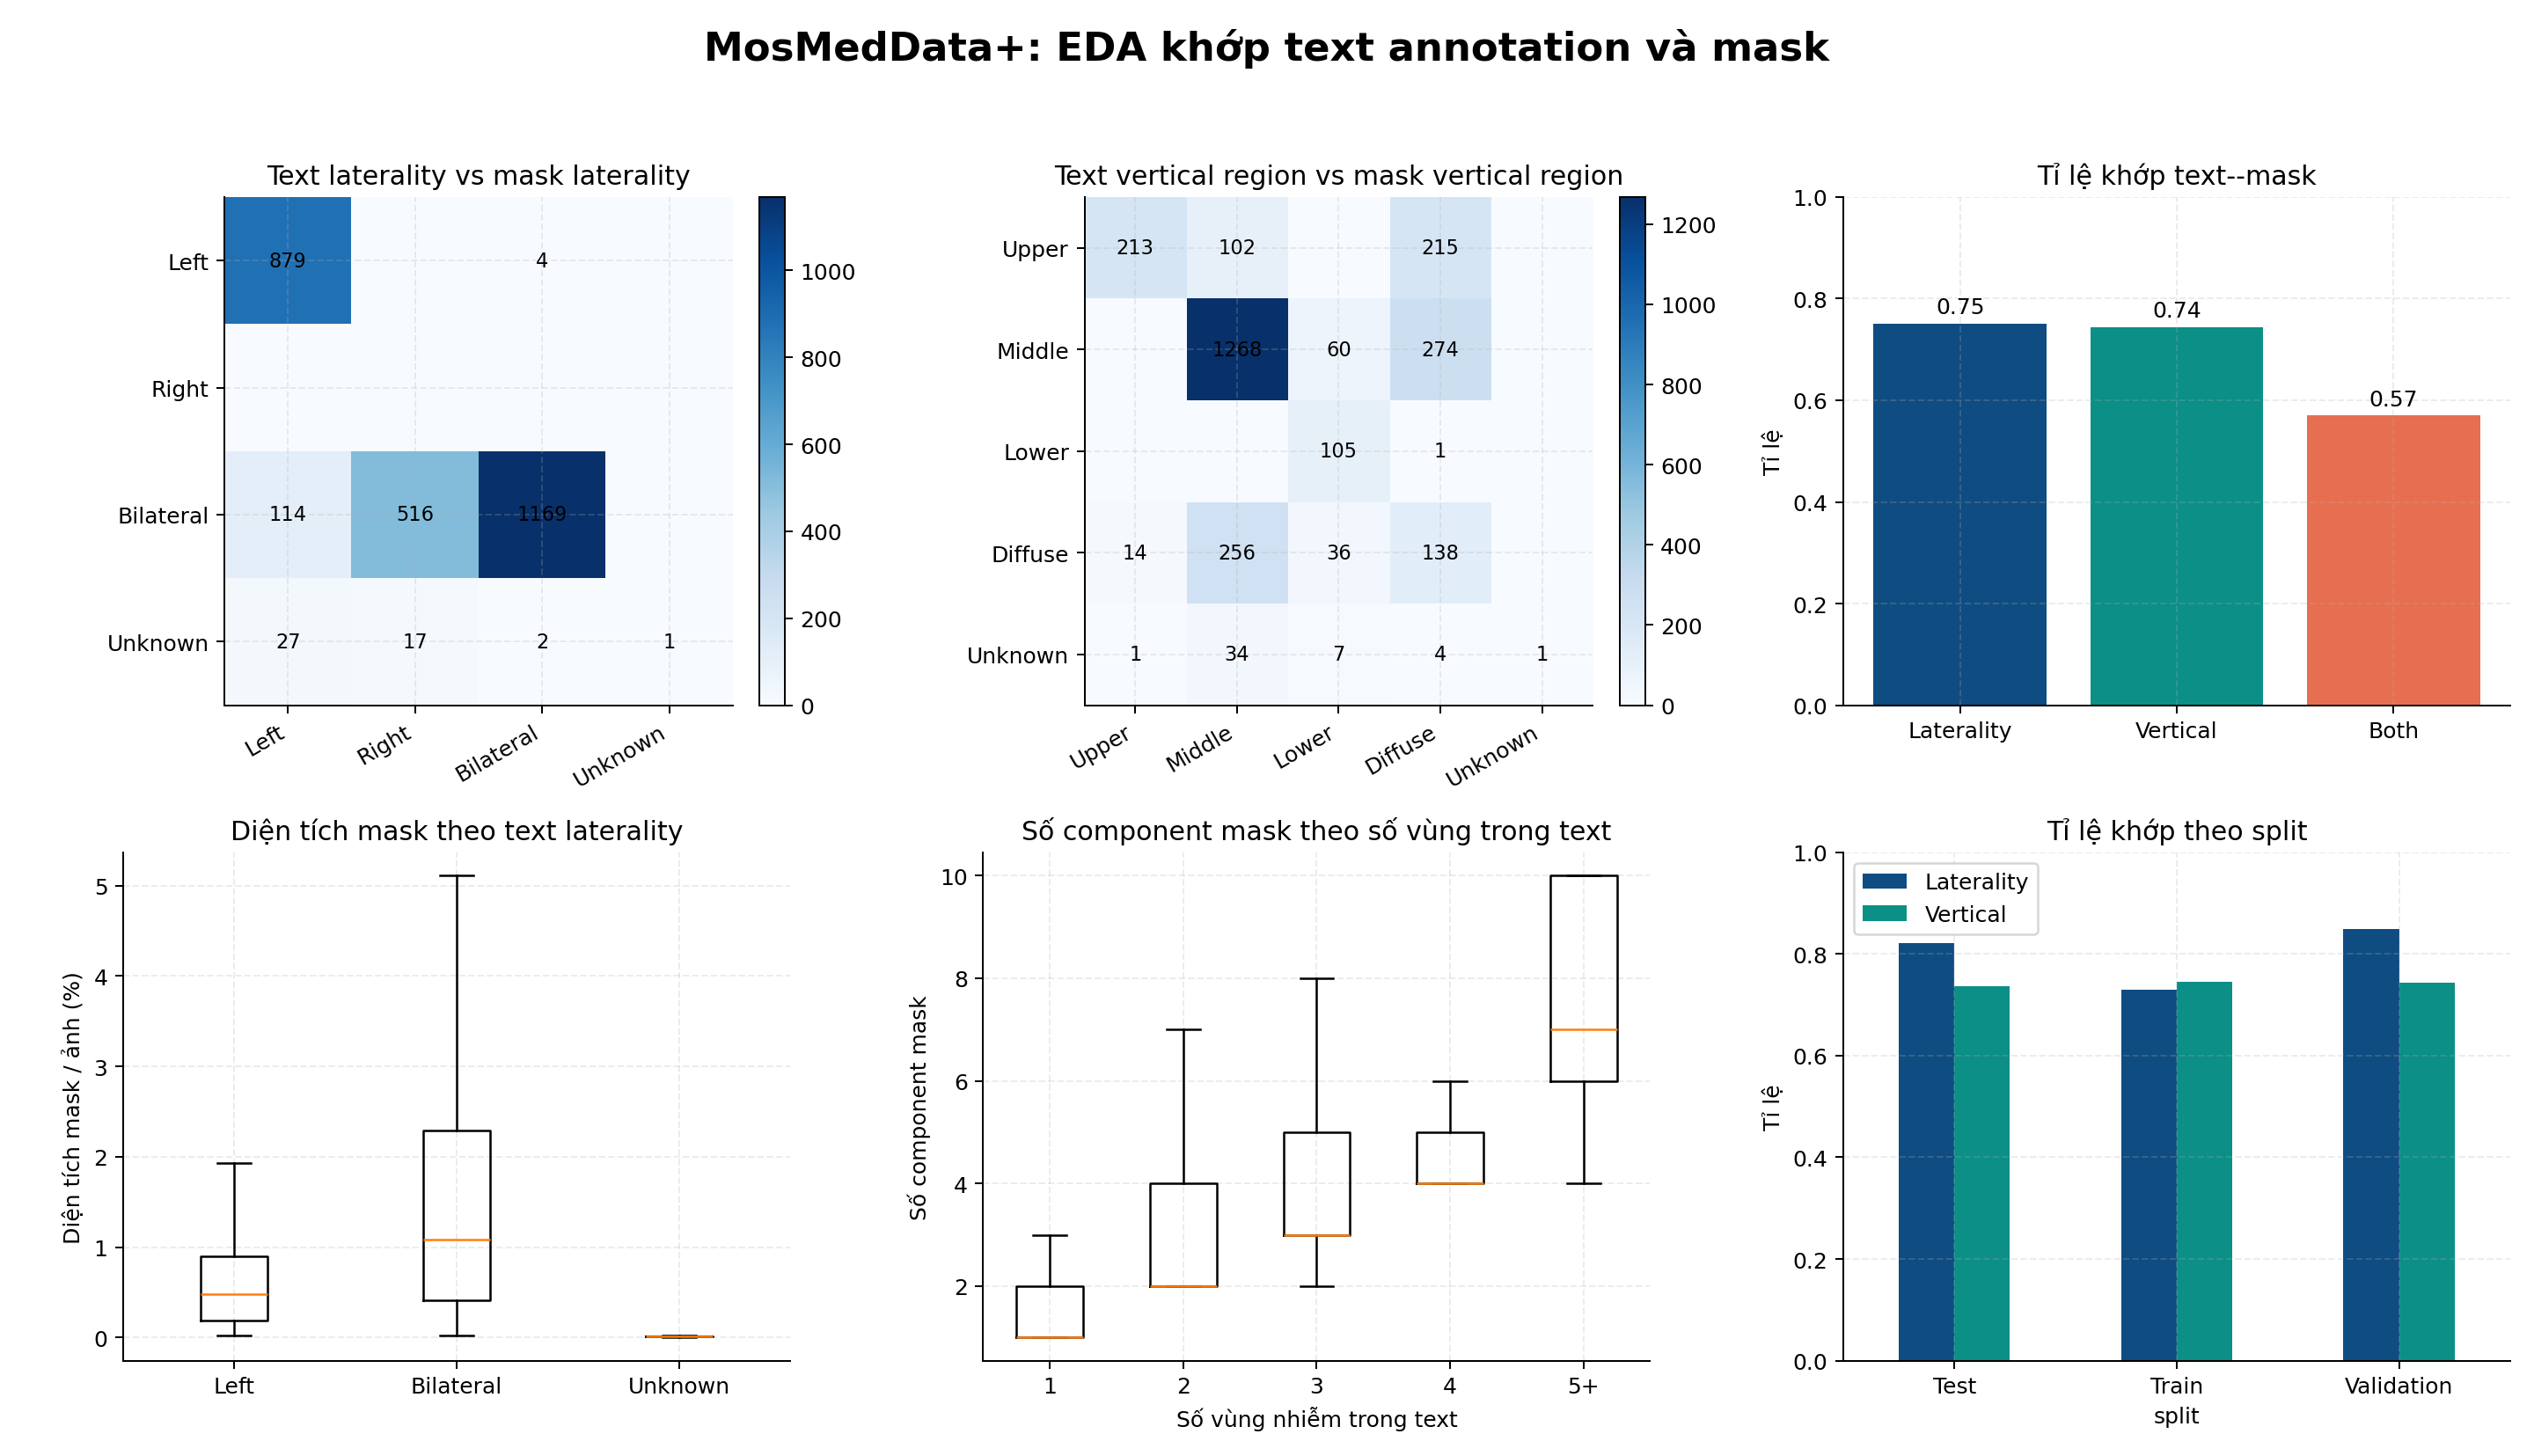
\includegraphics[width=0.96\textwidth]{figures/mosmed_text_mask_alignment.png}
  \caption{Đối sánh văn bản chú thích và mask của MosMedData+ theo trái/phải, tầng giải phẫu và số vùng nhiễm.}
  \label{fig:ch4-mosmed-văn bản-mask-alignment}
\end{figure}

Đối sánh văn bản--mask trên MosMedData+ cho kết quả yếu hơn QaTa-COV19 nhưng vẫn có cấu trúc đáng khai thác. Tỉ lệ khớp trái/phải đạt 75.05\%, tỉ lệ khớp tầng giải phẫu đạt 74.39\%, còn tỉ lệ khớp đồng thời cả hai chỉ đạt 56.98\%. Tương quan giữa số vùng nhiễm trong văn bản và số thành phần liên thông của mask là 0.442, thấp hơn rất nhiều so với QaTa-COV19. Sự khác biệt này phản ánh bản chất CT lát cắt và dữ liệu đa nguồn: văn bản có thể mô tả tình trạng vùng phổi ở mức ngữ nghĩa, trong khi mask chỉ biểu diễn những cụm tổn thương xuất hiện trên lát đang xét. Vì vậy, với MosMedData+, văn bản nên đóng vai trò điều hướng mềm chứ không nên trở thành ràng buộc cứng. Nếu LV loss hoặc pseudo-label bị đặt quá mạnh, mô hình có thể học theo mô tả tổng quát thay vì bằng chứng mức điểm ảnh của lát CT.

\textbf{Insight từ dữ liệu đa nguồn.} Vì MosMedData+ gộp từ nhiều nguồn CT, mô hình dễ gặp hai loại lệch phân bố. Lệch thứ nhất là lệch ảnh: cùng là CT phổi nhưng độ tương phản, vùng crop và nền ảnh khác nhau. Lệch thứ hai là lệch mô tả: văn bản chú thích có cùng khuôn ngữ với LViT nhưng quan hệ giữa câu mô tả và lát CT cụ thể không luôn mạnh như trên X-quang. Điều này giải thích vì sao một bộ mã hóa văn bản mạnh hơn chưa chắc tự động cho kết quả tốt hơn nếu pipeline ảnh và pseudo-label chưa ổn định. Ngược lại, một cấu hình văn bản nhẹ hơn nhưng có crop tốt, loss sạch và threshold hợp lý vẫn có thể cạnh tranh. Đây chính là tinh thần của các ablation MosMedData+: tách ảnh hưởng của tiền xử lý ảnh, học bán giám sát và mã hóa văn bản thay vì gộp tất cả vào một con số cuối.

\textbf{Insight dẫn sang thiết kế thử nghiệm.} MosMedData+ được dùng để kiểm tra độ bền của các cải tiến khi chuyển từ X-quang sang CT. Nếu QaTa-COV19 trả lời câu hỏi ``cải tiến có giúp LViT tận dụng văn bản và nhãn ít hơn không'', thì MosMedData+ trả lời câu hỏi ``cải tiến đó có còn đứng vững khi miền ảnh, mask và văn bản khó hơn không''. Vì vậy, phần sau ưu tiên các thí nghiệm crop-only, student-only, loss cleanup, LightAU, threshold cố định và bộ mã hóa văn bản nhẹ. Cách chia này giúp đọc kết quả MosMedData+ như một chuỗi phân tích nguyên nhân: tăng điểm đến từ xử lý ảnh, từ học bán giám sát, từ bộ mã hóa văn bản, hay từ hậu xử lý mask.

\begin{table}[H]
  \centering
  \caption{Từ EDA dữ liệu đến quyết định thử nghiệm trong Chương 4.}
  \label{tab:eda-to-experiment-decisions}
  \small
  \renewcommand{\arraystretch}{1.18}
  \setlength{\tabcolsep}{3pt}
  \begin{tabularx}{\textwidth}{@{}l Y Y Y@{}}
    \toprule
    Bộ dữ liệu & Quan sát EDA chính & Rủi ro nếu bỏ qua & Quyết định thử nghiệm tương ứng \\
    \midrule
    QaTa-COV19 & Mask trung vị 10.15\% ảnh, thường có 2 thành phần liên thông & Pseudo-label phải giữ cấu trúc tổn thương hai bên, không chỉ sinh một vùng foreground lớn & Đánh giá 25\%, 50\%, 100\% nhãn; kiểm tra EPI/LV loss \\
    QaTa-COV19 & văn bản khớp trái/phải 95.68\%, tương quan số vùng với component đạt 0.911 & Bỏ văn bản sẽ mất tín hiệu giải phẫu mạnh; nhưng văn bản vẫn không thay mask mức điểm ảnh & Thử prompt normalization, BiomedBERT và NoBERT/BiGRU \\
    QaTa-COV19 & Tâm mask cân bằng gần giữa ảnh, trái/phải có ý nghĩa rõ & Augmentation hình học có thể làm mâu thuẫn ảnh--văn bản & Hạn chế biến đổi phá vỡ định hướng giải phẫu; giữ bố cục toàn phổi \\
    MosMedData+ & CT đa nguồn, cường độ và trường nhìn không đồng nhất & Mô hình học nhiễu nền hoặc phụ thuộc nguồn dữ liệu & Thử crop vùng phổi, chuẩn hóa cường độ và LightAU \\
    MosMedData+ & Mask trung vị 0.758\% ảnh, 58.54\% mẫu nhỏ hơn 1\%, phân vị 95 của component là 17 & Dice/IoU thay đổi mạnh theo nhị phân hóa; dễ bỏ sót cụm nhỏ & So sánh threshold cố định/threshold validation và loss cleanup \\
    MosMedData+ & văn bản--mask khớp đồng thời chỉ 56.98\%, tương quan số vùng với component đạt 0.442 & Văn bản có thể hỗ trợ sai mức nếu áp quá mạnh vào từng lát CT & Đọc văn bản như tín hiệu bổ trợ; so sánh bộ mã hóa văn bản nhẹ và bộ mã hóa y sinh \\
    \bottomrule
  \end{tabularx}
\end{table}
\FloatBarrier

\section{Quy trình thử nghiệm}

Quy trình thử nghiệm được thiết kế để biến phương pháp ở Chương 3 thành các câu hỏi có thể kiểm chứng. Tinh thần chung không phải chạy một mô hình rồi báo cáo một con số, mà là tách từng nhóm ẩn số của hệ thống: LViT gốc mạnh ở đâu, văn bản chú thích đóng góp thế nào, pseudo-label có giúp khi thiếu mask hay không, tiền xử lý ảnh ảnh hưởng ra sao, và các cải tiến có còn ổn định khi chuyển từ X-quang sang CT hay không. Vì vậy, phần này bắt đầu bằng tổng quan thiết kế thực nghiệm và thiết lập LViT, sau đó mới đi vào quy trình riêng cho QaTa-COV19 và MosMedData+.

\subsection{Tổng quan thiết kế thực nghiệm}

Trọng tâm đầu tiên của thử nghiệm là LViT. Trước khi bàn về cải tiến, cần xác định LViT được vận hành theo một pipeline đầy đủ: ảnh và văn bản được đọc theo từng mẫu; ảnh được chuẩn hóa về cùng kích thước; văn bản chú thích được mã hóa thành vector/token; mô hình sinh mặt nạ xác suất; mask dự đoán được tối ưu bằng loss ở giai đoạn học và được đối sánh với ground truth ở giai đoạn đánh giá. Khi chỉ một phần dữ liệu có mask thật, phần còn lại được đưa vào nhánh học bán giám sát để kiểm tra giá trị của pseudo-label và ràng buộc ảnh--văn bản.

Báo cáo tổ chức thử nghiệm theo bốn nhóm. Nhóm thứ nhất là \textit{tái hiện và đặt mốc LViT}: dùng kết quả LViT gốc làm baseline phương pháp, nhấn mạnh kiến trúc Double-U, LV Fusion, PLAM, EPI và LV loss. Nhóm thứ hai là \textit{thử nghiệm theo tỉ lệ nhãn}: 25\%, 50\%, 100\% trên QaTa-COV19 để trả lời câu hỏi khi mask chuyên gia giảm thì văn bản/pseudo-label còn giúp bao nhiêu. Nhóm thứ ba là \textit{ablation cải tiến}: chuẩn hóa prompt, bộ mã hóa văn bản, cơ chế fusion, loss và pseudo-label được thay đổi có kiểm soát để biết thành phần nào thật sự tạo ra chênh lệch. Nhóm thứ tư là \textit{kiểm tra chuyển miền}: MosMedData+ được dùng để xem những kết luận từ X-quang có còn giữ được khi sang CT hay không.

\begin{table}[H]
  \centering
  \caption{Các nhóm thử nghiệm và ẩn số cần trả lời.}
  \label{tab:experiment-questions}
  \small
  \renewcommand{\arraystretch}{1.16}
  \setlength{\tabcolsep}{4pt}
  \begin{tabularx}{\textwidth}{@{}p{0.21\textwidth} Y Y Y@{}}
    \toprule
    Nhóm thử nghiệm & Ẩn số cần trả lời & Cách kiểm tra & Cách đọc kết quả \\
    \midrule
    Mốc LViT & LViT có lợi thế gì so với mạng phân đoạn ảnh thuần? & Đặt kết quả LViT gốc cạnh các baseline CNN/U-Net và dùng cùng Dice/IoU & Nếu LViT tốt hơn, văn bản và hybrid CNN--Transformer có giá trị thực nghiệm \\
    Tỉ lệ nhãn & Khi mask thật ít đi, hệ thống còn học được nhờ văn bản/pseudo-label không? & Chạy 25\%, 50\%, 100\% nhãn trên QaTa-COV19 & Chênh lệch lớn ở 25\%/50\% cho thấy cải tiến hữu ích trong bối cảnh ít nhãn \\
    bộ mã hóa văn bản & Có cần bộ mã hóa ngôn ngữ sâu, hay văn bản có cấu trúc chỉ cần embedding/chuẩn hóa tốt? & So sánh prompt chưa chuẩn hóa, prompt normalization, BiomedBERT và NoBERT/BiGRU & Nếu văn bản nhẹ vẫn cạnh tranh, cấu trúc chú thích quan trọng không kém độ sâu bộ mã hóa \\
    Pseudo-label và loss & Nhãn giả giúp học thêm hay làm lan truyền sai số? & So sánh EPI/LV loss của LViT với student-only, loss cleanup, confidence mask, consistency, boundary và prototype alignment & Kết quả cần đọc cùng ổn định validation và chất lượng mask xác suất \\
    Chuyển miền CT & Cải tiến trên X-quang có còn đúng trên CT không? & Kiểm tra MosMedData+ với crop vùng phổi, student-only, loss cleanup, LightAU và ngưỡng đánh giá cố định & Nếu điểm nhạy với crop/augmentation/ngưỡng, giới hạn nằm ở miền ảnh và hậu xử lý, không chỉ ở văn bản \\
    \bottomrule
  \end{tabularx}
\end{table}
\FloatBarrier

\subsection{Thiết lập LViT và cấu hình huấn luyện}

Thiết lập LViT gốc được xem như mốc phương pháp. Ảnh đầu vào được đưa về \(224\times224\), số kênh ảnh là 3, đầu ra là một mask nhị phân. Khối Transformer trong CTrans/LViT dùng bốn mức patch \([16,8,4,2]\), bốn head attention, bốn layer Transformer, tỉ lệ mở rộng MLP bằng 4, dropout attention/embedding bằng 0.1 và base channel của U-Net bằng 64. Những tham số này phản ánh triết lý của LViT: CNN giữ bản đồ đặc trưng nhiều mức, Transformer học ngữ cảnh xa trên token đa tỉ lệ, còn văn bản được đưa vào để điều chỉnh biểu diễn ảnh trước khi giải mã phân đoạn.

Ở huấn luyện có giám sát của LViT, loss chính là kết hợp Dice và BCE. Dice loss phù hợp với phân đoạn tổn thương vì foreground thường nhỏ hơn nền rất nhiều; BCE giúp từng điểm ảnh có xác suất đúng hơn. Optimizer của cấu hình LViT gốc là Adam, batch size mặc định là 16, seed là 666, và lịch học dùng cosine warm restart khi bật cosine learning rate. Với bài toán COVID-19, learning rate được đặt ở mức \(3\times10^{-4}\) trong ghi chú cấu hình, còn ảnh và mask được tăng cường bằng các phép xoay/lật hoặc xoay góc nhỏ ở train, trong khi validation chỉ resize/chuẩn hóa. Cơ chế chọn mô hình dựa trên Dice validation tốt nhất, nhờ vậy kết quả test được đọc từ checkpoint ổn định nhất thay vì epoch cuối.

\begin{table}[H]
  \centering
  \caption{Thiết lập chính của LViT gốc dùng làm mốc phương pháp.}
  \label{tab:lvit-original-training-setup}
  \small
  \renewcommand{\arraystretch}{1.15}
  \setlength{\tabcolsep}{4pt}
  \begin{tabularx}{\textwidth}{@{}p{0.28\textwidth} Y@{}}
    \toprule
    Thành phần & Thiết lập \\
    \midrule
    Kích thước ảnh & \(224\times224\) \\
    Số kênh / số lớp đầu ra & 3 kênh ảnh, 1 lớp mask nhị phân \\
    Backbone thị giác & Double-U/CNN bộ mã hóa--bộ giải mã với base channel 64 \\
    Transformer đa mức & Patch sizes \([16,8,4,2]\), 4 attention heads, 4 layers, MLP expand ratio 4 \\
    Dropout Transformer & Embedding dropout 0.1, attention dropout 0.1 \\
    Loss có giám sát & Weighted Dice + BCE, hai thành phần được dùng cùng nhau để xử lý mất cân bằng foreground/background \\
    Optimizer và batch & Adam, batch size 16 trong cấu hình gốc \\
    Learning rate & \(3\times10^{-4}\) cho thiết lập COVID-19; cosine warm restart với \(T_0=10\) và \(\eta_{\min}=10^{-4}\) \\
    Seed và chọn checkpoint & Seed 666; chọn checkpoint theo Dice validation tốt nhất \\
    Tăng cường dữ liệu & Resize về kích thước chuẩn; train có xoay/lật hoặc xoay góc nhỏ, validation giữ biến đổi xác định \\
    \bottomrule
  \end{tabularx}
\end{table}
\FloatBarrier

Trên nền LViT đó, phần cải tiến được thiết kế như một chuỗi kiểm tra có kiểm soát hơn là một thay đổi đơn lẻ. Để tránh hiểu QaTaLViT như một tên gọi mơ hồ, có thể tóm tắt mô hình cải tiến theo năm nhóm module. Nhóm thứ nhất là \textbf{chuẩn hóa văn bản}: văn bản chú thích được đưa về dạng nhất quán hơn trước khi mã hóa, nhằm giảm trường hợp hai câu cùng nghĩa nhưng được viết khác nhau. Nhóm thứ hai là \textbf{mã hóa văn bản y sinh}: cấu hình chính dùng BiomedBERT để tạo embedding 768 chiều, còn cấu hình NoBERT dùng embedding học từ đầu và BiGRU để kiểm tra phương án nhẹ hơn. Nhóm thứ ba là \textbf{hợp nhất ảnh--văn bản}: đặc trưng ảnh từ bộ mã hóa được điều chỉnh bằng tín hiệu văn bản qua các khối fusion/cross-modal interaction thay vì chỉ nối vector văn bản ở cuối mạng. Nhóm thứ tư là \textbf{prior không gian và skip adapter}: văn bản được biến thành gợi ý mềm về vị trí/vùng tổn thương, đồng thời skip đặc trưng trong bộ giải mã được điều chỉnh để hạn chế truyền thẳng nhiễu thị giác. Nhóm thứ năm là \textbf{kiểm soát nhãn giả}: pseudo-label được xem là tín hiệu tạm, cần lọc bằng độ tin cậy, consistency, boundary/prototype alignment và EMA/EPI khi có dữ liệu chưa nhãn.

\begin{table}[H]
  \centering
  \caption{Các nhóm module trong mô hình QaTaLViT cải tiến.}
  \label{tab:qatalvit-module-summary}
  \small
  \renewcommand{\arraystretch}{1.15}
  \setlength{\tabcolsep}{4pt}
  \begin{tabularx}{\textwidth}{@{}p{0.24\textwidth} Y Y@{}}
    \toprule
    Nhóm module & Vai trò trong pipeline & Lý do kiểm tra trong thực nghiệm \\
    \midrule
    Prompt/văn bản normalization & Chuẩn hóa câu mô tả thành tín hiệu ngữ nghĩa ổn định trước khi mã hóa & Nếu văn bản nhiễu, fusion có thể làm mô hình kém hơn baseline ảnh--văn bản gốc \\
    bộ mã hóa văn bản & BiomedBERT hoặc NoBERT/BiGRU biến văn bản thành vector/token dùng được bởi mạng phân đoạn & Kiểm tra văn bản cần pretrained y sinh sâu hay chỉ cần bộ mã hóa nhẹ trên văn bản có cấu trúc \\
    Cross-modal fusion & Đưa embedding văn bản vào đặc trưng ảnh ở các tầng mã hóa/thân mạng & Kiểm tra văn bản có giúp điều chỉnh biểu diễn ảnh trước bộ giải mã hay không \\
    Spatial prior và skip adapter & Tạo gợi ý không gian mềm từ văn bản và điều chỉnh skip đặc trưng khi giải mã & Giảm dự đoán lan rộng, bỏ sót cụm nhỏ và truyền nhiễu nền qua skip connection \\
    Pseudo-label control & Lọc nhãn giả bằng confidence/consistency, EMA/EPI và các ràng buộc phụ trợ & Hạn chế việc dữ liệu chưa nhãn khuếch đại sai số khi mask thật ít \\
    Training recipe & AdamW, cosine scheduler, gradient accumulation, augmentation có kiểm soát & Tách tác động của module khỏi nhiễu do huấn luyện không ổn định \\
    \bottomrule
  \end{tabularx}
\end{table}
\FloatBarrier

Thiết lập chính dùng ảnh \(224\times224\), 120 epoch, batch size 4 kết hợp gradient accumulation 4 bước nên batch hiệu dụng là 16, optimizer AdamW, learning rate \(10^{-4}\), weight decay \(10^{-4}\), cosine scheduler với \(\eta_{\min}=10^{-6}\), seed 666, 2 worker đọc dữ liệu và AMP mixed precision. Nhánh teacher/student trong học bán giám sát dùng EMA decay 0.99. văn bản chú thích được chia tối đa 10 đơn vị ngữ nghĩa; cấu hình y sinh dùng BiomedBERT để lấy embedding 768 chiều, còn các ablation nhẹ hơn kiểm tra giả thuyết rằng văn bản có cấu trúc mạnh có thể không cần bộ mã hóa quá sâu.

\begin{table}[H]
  \centering
  \caption{Thiết lập chính của các thử nghiệm cải tiến trên nền LViT.}
  \label{tab:qatalvit-training-setup}
  \small
  \renewcommand{\arraystretch}{1.15}
  \setlength{\tabcolsep}{4pt}
  \begin{tabularx}{\textwidth}{@{}p{0.28\textwidth} Y@{}}
    \toprule
    Thành phần & Thiết lập \\
    \midrule
    Epoch và batch & 120 epoch; batch size 4; gradient accumulation 4; batch hiệu dụng 16 \\
    Optimizer / scheduler & AdamW; cosine scheduler; \(lr=10^{-4}\), \(\eta_{\min}=10^{-6}\), weight decay \(10^{-4}\) \\
    Seed, workers và AMP & Seed 666; 2 worker đọc dữ liệu; AMP mixed precision \\
    bộ mã hóa văn bản chính & BiomedBERT, embedding 768 chiều, tối đa 10 văn bản units mỗi mẫu \\
    Học bán giám sát & Chia train thành phần có nhãn và chưa nhãn theo label ratio; dùng teacher/student với EMA decay 0.99 \\
    Tỉ lệ nhãn QaTa-COV19 & 25\%, 50\%, 100\% để kiểm tra vai trò của mask thật, văn bản và pseudo-label \\
    Đánh giá validation & QaTa-COV19 dùng ngưỡng cố định \(\tau=0.5\); MosMedData+ báo cáo tách riêng fixed-threshold và validation-threshold \\
    Các ablation chính & Thay đổi từng nhóm module: chuẩn hóa prompt, bộ mã hóa văn bản, fusion ảnh--văn bản, prior/skip adapter, kiểm soát pseudo-label, crop/augmentation và loss cleanup \\
    \bottomrule
  \end{tabularx}
\end{table}
\FloatBarrier

\begin{table}[H]
  \centering
  \caption{Độ phức tạp suy luận tương đối của baseline LViT và mô hình cải tiến.}
  \label{tab:complexity-comparison}
  \small
  \renewcommand{\arraystretch}{1.15}
  \setlength{\tabcolsep}{4pt}
  \begin{tabularx}{\textwidth}{@{}p{0.32\textwidth} Y Y Y@{}}
    \toprule
    Mô hình & Số tham số & FLOPs & Cách đọc kết quả \\
    \midrule
    LViT gốc (mốc phương pháp) & 29.72M & 27.08 GFLOPs & Mốc gốc của LViT với nhánh ảnh--văn bản và backbone Double-U + Transformer. \\
    QaTaLViT cải tiến & 25.93M & 33.67 GFLOPs & Giảm số tham số nhưng tăng chi phí phép tính do các khối tương tác ảnh--văn bản/phụ trợ trong pipeline cải tiến. \\
    \bottomrule
  \end{tabularx}
\end{table}

\noindent Các số trên được đo trên cùng giao thức: một mẫu đầu vào ảnh \(1\times3\times224\times224\) và văn bản tối đa 10 đơn vị ngữ nghĩa đã mã hóa thành tensor \(1\times10\times768\). Vì vậy, bảng này nên được đọc như chi phí suy luận tương đối giữa hai cấu hình trong cùng báo cáo, không phải benchmark tuyệt đối giữa mọi phần cứng/phần mềm.
\FloatBarrier

Từ đây trở xuống, quy trình được tách theo từng bộ dữ liệu vì QaTa-COV19 và MosMedData+ khác nhau về miền ảnh, tiền xử lý, độ ổn định của văn bản chú thích và cách đọc kết quả.

\subsection{QaTa-COV19}

\textbf{Tiền xử lý dữ liệu.} Ảnh X-quang được đưa về cùng kích thước đầu vào, chuẩn hóa cường độ và chuyển về tensor. Mask được resize đồng bộ với ảnh và giữ dạng nhị phân để tính loss/metric. Với QaTa-COV19, cần giữ cấu trúc toàn phổi vì vị trí trái/phải và upper/middle/lower trong văn bản có ý nghĩa giải phẫu. Văn bản được chuẩn hóa ở mức prompt/văn bản chú thích trước khi mã hóa để giảm nhiễu hình thức và giúp các mô tả cùng nghĩa có biểu diễn ổn định hơn.

\textbf{Huấn luyện mô hình.} Trong nhánh có nhãn, mô hình nhận \((x,t,y)\), sinh \(\hat{y}\), rồi tối ưu loss giữa \(\hat{y}\) và \(y\). Loss chính kết hợp BCE và Dice để vừa học xác suất từng điểm ảnh, vừa tối ưu độ chồng lấp vùng. Trong nhánh chưa nhãn, mô hình nhận \((x,t)\), sinh dự đoán, tạo pseudo-label và dùng loss chưa nhãn để tận dụng thêm dữ liệu không có mask chuyên gia. Các mức nhãn 25\%, 50\%, 100\% được dùng để quan sát vai trò của văn bản và pseudo-label khi lượng mask thay đổi.

\textbf{Sinh mặt nạ và đối sánh ground truth.} Mô hình sinh bản đồ xác suất \(\hat{y}\in[0,1]^{H\times W}\), sau đó nhị phân hóa bằng ngưỡng \(\tau\) để thu được mask dự đoán. Với QaTa-COV19, toàn bộ bảng chính dùng ngưỡng cố định \(\tau=0.5\) để giữ phép so sánh công bằng giữa baseline, cải tiến và các ablation. Mask dự đoán được so với ground truth bằng Dice và IoU.

\subsection{MosMedData+}

\textbf{Tiền xử lý dữ liệu.} Ảnh CT được đưa về cùng kích thước đầu vào và chuẩn hóa cường độ. Khác với QaTa-COV19, MosMedData+ nhạy hơn với crop hoặc chuẩn hóa vùng phổi vì CT có nhiều nền ngoài phổi và phân bố cường độ thay đổi theo nguồn dữ liệu. Các thử nghiệm cho thấy crop-only và augmentation nhẹ có ảnh hưởng rõ đến kết quả, nên tiền xử lý trên MosMedData+ không thể xem là chi tiết phụ.

\textbf{Huấn luyện mô hình.} MosMedData+ được chạy ở ba mức 25\%, 50\% và 100\% nhãn để kiểm tra khả năng chuyển miền khi lượng mask chuyên gia thay đổi. Quy trình huấn luyện vẫn nhận \((x,t,y)\) ở mẫu có nhãn và \((x,t)\) ở mẫu chưa nhãn, nhưng cấu hình chính trên MosMedData+ nhấn mạnh student-only, loss cleanup, crop vùng phổi và augmentation nhẹ kiểu nnU-Net. Cách tổ chức này phản ánh khác biệt quan trọng: cơ chế bán giám sát tốt trên X-quang không nhất thiết hoạt động giống hệt trên CT, nơi mask nhỏ, phân mảnh và nhạy với tiền xử lý hơn.

\textbf{Sinh mặt nạ và đối sánh ground truth.} Với MosMedData+, bản đồ xác suất đầu ra nhạy hơn với ngưỡng nhị phân hóa. Vì vậy, báo cáo chủ động tách hai kiểu đánh giá. Kiểu thứ nhất là \textit{fixed-threshold}, đặt \(\tau=0.5\) cho mọi cấu hình để so sánh trực tiếp với QaTa-COV19 và giữa các recipe CT. Kiểu thứ hai là \textit{validation-threshold}, chọn một ngưỡng duy nhất trên validation cho từng cấu hình rồi khóa ngưỡng đó khi chạy test. Cách tách này giúp người đọc phân biệt rõ cải thiện đến từ bản thân mô hình hay từ việc calibrate ngưỡng đầu ra. Sau khi nhị phân hóa, mask dự đoán được đối sánh với ground truth bằng Dice và IoU. Kết quả cần được đọc trong bối cảnh chuyển miền từ X-quang sang CT: một thay đổi nhỏ ở vùng xác suất biên có thể làm mất các cụm tổn thương nhỏ hoặc sinh false positive quanh rìa phổi.

\subsection{Tiêu chí đánh giá chung}

Sau khi có mask dự đoán, hệ thống đối sánh \(\hat{Y}\) với ground truth \(Y\). Về trực giác, phần giao \(Y\cap\hat{Y}\) là vùng mô hình dự đoán đúng, còn phần hợp \(Y\cup\hat{Y}\) là toàn bộ vùng được xem là liên quan bởi mask thật hoặc mask dự đoán. Hình~\ref{fig:dice-iou-comparison} minh họa cách đọc hai đại lượng này trước khi đi vào công thức.

\begin{figure}[H]
  \centering
  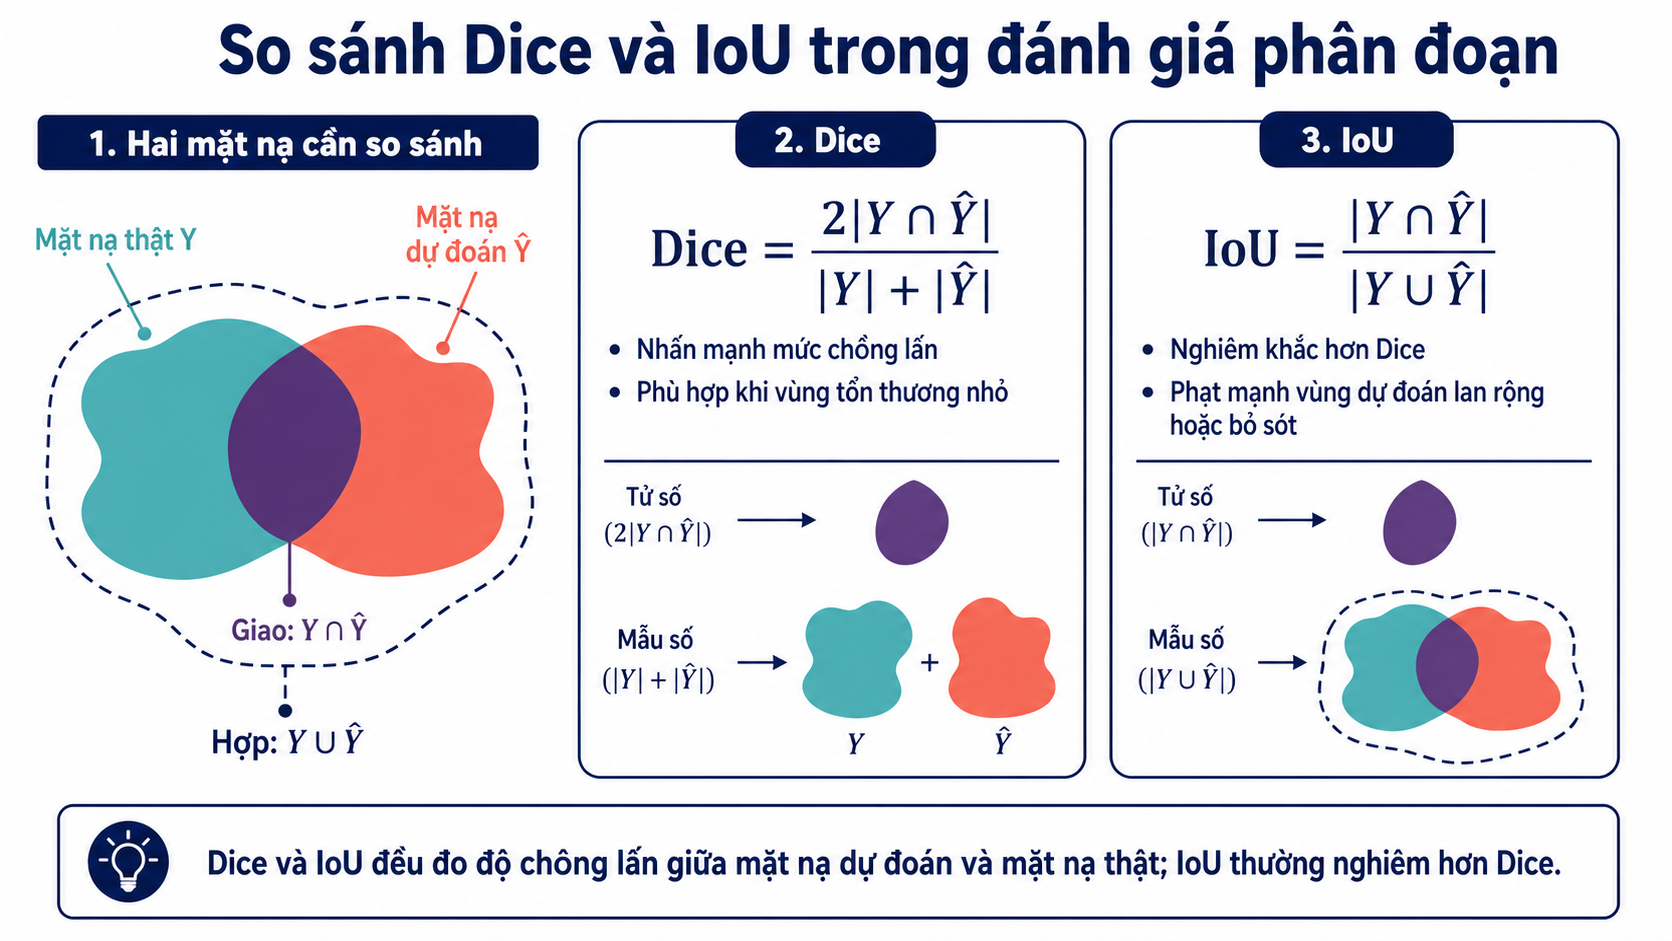
\includegraphics[width=0.96\textwidth]{figures/dice_iou_comparison_generated.png}
  \caption{So sánh Dice và IoU trong đánh giá phân đoạn. Vùng tím biểu diễn phần giao giữa mặt nạ thật và mặt nạ dự đoán; đường viền đứt biểu diễn phần hợp. Dice nhân đôi phần giao rồi chia cho tổng diện tích hai mask, còn IoU chia phần giao cho phần hợp nên thường nghiêm khắc hơn khi mô hình dự đoán lan rộng hoặc bỏ sót vùng tổn thương.}
  \label{fig:dice-iou-comparison}
\end{figure}

Hai độ đo chính được dùng trong báo cáo là:
\[
\mathrm{Dice}=\frac{2|Y\cap \hat{Y}|}{|Y|+|\hat{Y}|},
\qquad
\mathrm{IoU}=\frac{|Y\cap \hat{Y}|}{|Y\cup \hat{Y}|}.
\]
Dice nhấn mạnh mức chồng lấp giữa hai vùng, còn IoU nghiêm khắc hơn vì mẫu số là hợp của vùng thật và vùng dự đoán. Với phân đoạn y khoa, cần nhìn cả hai: Dice cao cho thấy vùng dự đoán phủ tốt vùng thật, còn IoU giúp phát hiện trường hợp mô hình dự đoán quá rộng hoặc quá lệch.

\section{Kết quả thực nghiệm}

Phần kết quả cũng được chia theo từng bộ dữ liệu. QaTa-COV19 là tập chính để kiểm tra cải tiến theo tỉ lệ nhãn, còn MosMedData+ là tập mở rộng để kiểm tra chuyển miền sang CT. Trong mỗi bộ dữ liệu, báo cáo đặt mốc LViT gốc trước rồi mới trình bày kết quả cải tiến hoặc ablation tương ứng.

\subsection{QaTa-COV19}

\textbf{Mốc LViT gốc và kết quả chạy lại baseline.} Trên QaTa-COV19, tài liệu chính thức báo cáo U-Net đạt 79.02 Dice và 69.46 IoU, còn LViT-T đạt 83.66 Dice và 75.11 IoU \cite{lvitOfficialRepo}. Mốc này cho thấy hướng ảnh--văn bản của LViT đã có lợi thế so với CNN thuần trên ảnh X-quang COVID-19. Tuy nhiên, để báo cáo không chỉ dựa vào con số trong tài liệu gốc, nhóm cũng phân tích các lần chạy lại LViT ở bối cảnh 25\%, 50\% và 100\% nhãn. Ba mức này cho phép nhìn rõ câu hỏi trung tâm của LViT: khi tăng số mask chuyên gia, hệ thống ảnh--văn bản và pseudo-label ổn định hơn như thế nào.

\begin{table}[H]
  \centering
  \caption{Kết quả chạy lại LViT baseline trên QaTa-COV19 với 25\%, 50\% và 100\% nhãn.}
  \label{tab:lvit-baseline-rerun-25-50}
  \small
  \renewcommand{\arraystretch}{1.12}
  \begin{tabularx}{\textwidth}{@{}l l r r r r@{}}
    \toprule
    Tỉ lệ nhãn & Split & Số mẫu & Accuracy & Dice & IoU \\
    \midrule
    25\% & Train & 5716 & 96.24 & 78.45 & 68.01 \\
    25\% & Validation & 1429 & 95.99 & 76.49 & 65.61 \\
    25\% & Test & 2113 & 96.62 & 78.42 & 68.43 \\
    \midrule
    50\% & Train & 5716 & 96.62 & 81.47 & 71.46 \\
    50\% & Validation & 1429 & 96.29 & 79.11 & 68.48 \\
    50\% & Test & 2113 & 96.84 & 80.32 & 70.60 \\
    \midrule
    100\% & Train & 5716 & 97.54 & 86.58 & 77.88 \\
    100\% & Validation & 1429 & 96.88 & 81.21 & 71.24 \\
    100\% & Test & 2113 & 97.43 & 82.76 & 73.78 \\
    \bottomrule
  \end{tabularx}
\end{table}
\FloatBarrier

Bảng~\ref{tab:lvit-baseline-rerun-25-50} cho thấy khi tăng nhãn từ 25\% lên 50\%, LViT baseline tăng từ 78.42 lên 80.32 Dice trên test, và IoU tăng từ 68.43 lên 70.60. Khi dùng 100\% nhãn, test Dice đạt 82.76 và IoU đạt 73.78. Xu hướng này hợp lý: càng nhiều mask thật, supervised loss càng có thêm neo tin cậy, pseudo-label ít phải gánh toàn bộ tín hiệu học. Điểm validation cũng tăng từ 76.49 lên 79.11 rồi 81.21 Dice. Accuracy đều trên 95\%, song accuracy không đủ để kết luận tốt vì nền ảnh chiếm phần lớn điểm ảnh. Do đó, Dice và IoU vẫn là hai độ đo chính.

\begin{figure}[H]
  \centering
  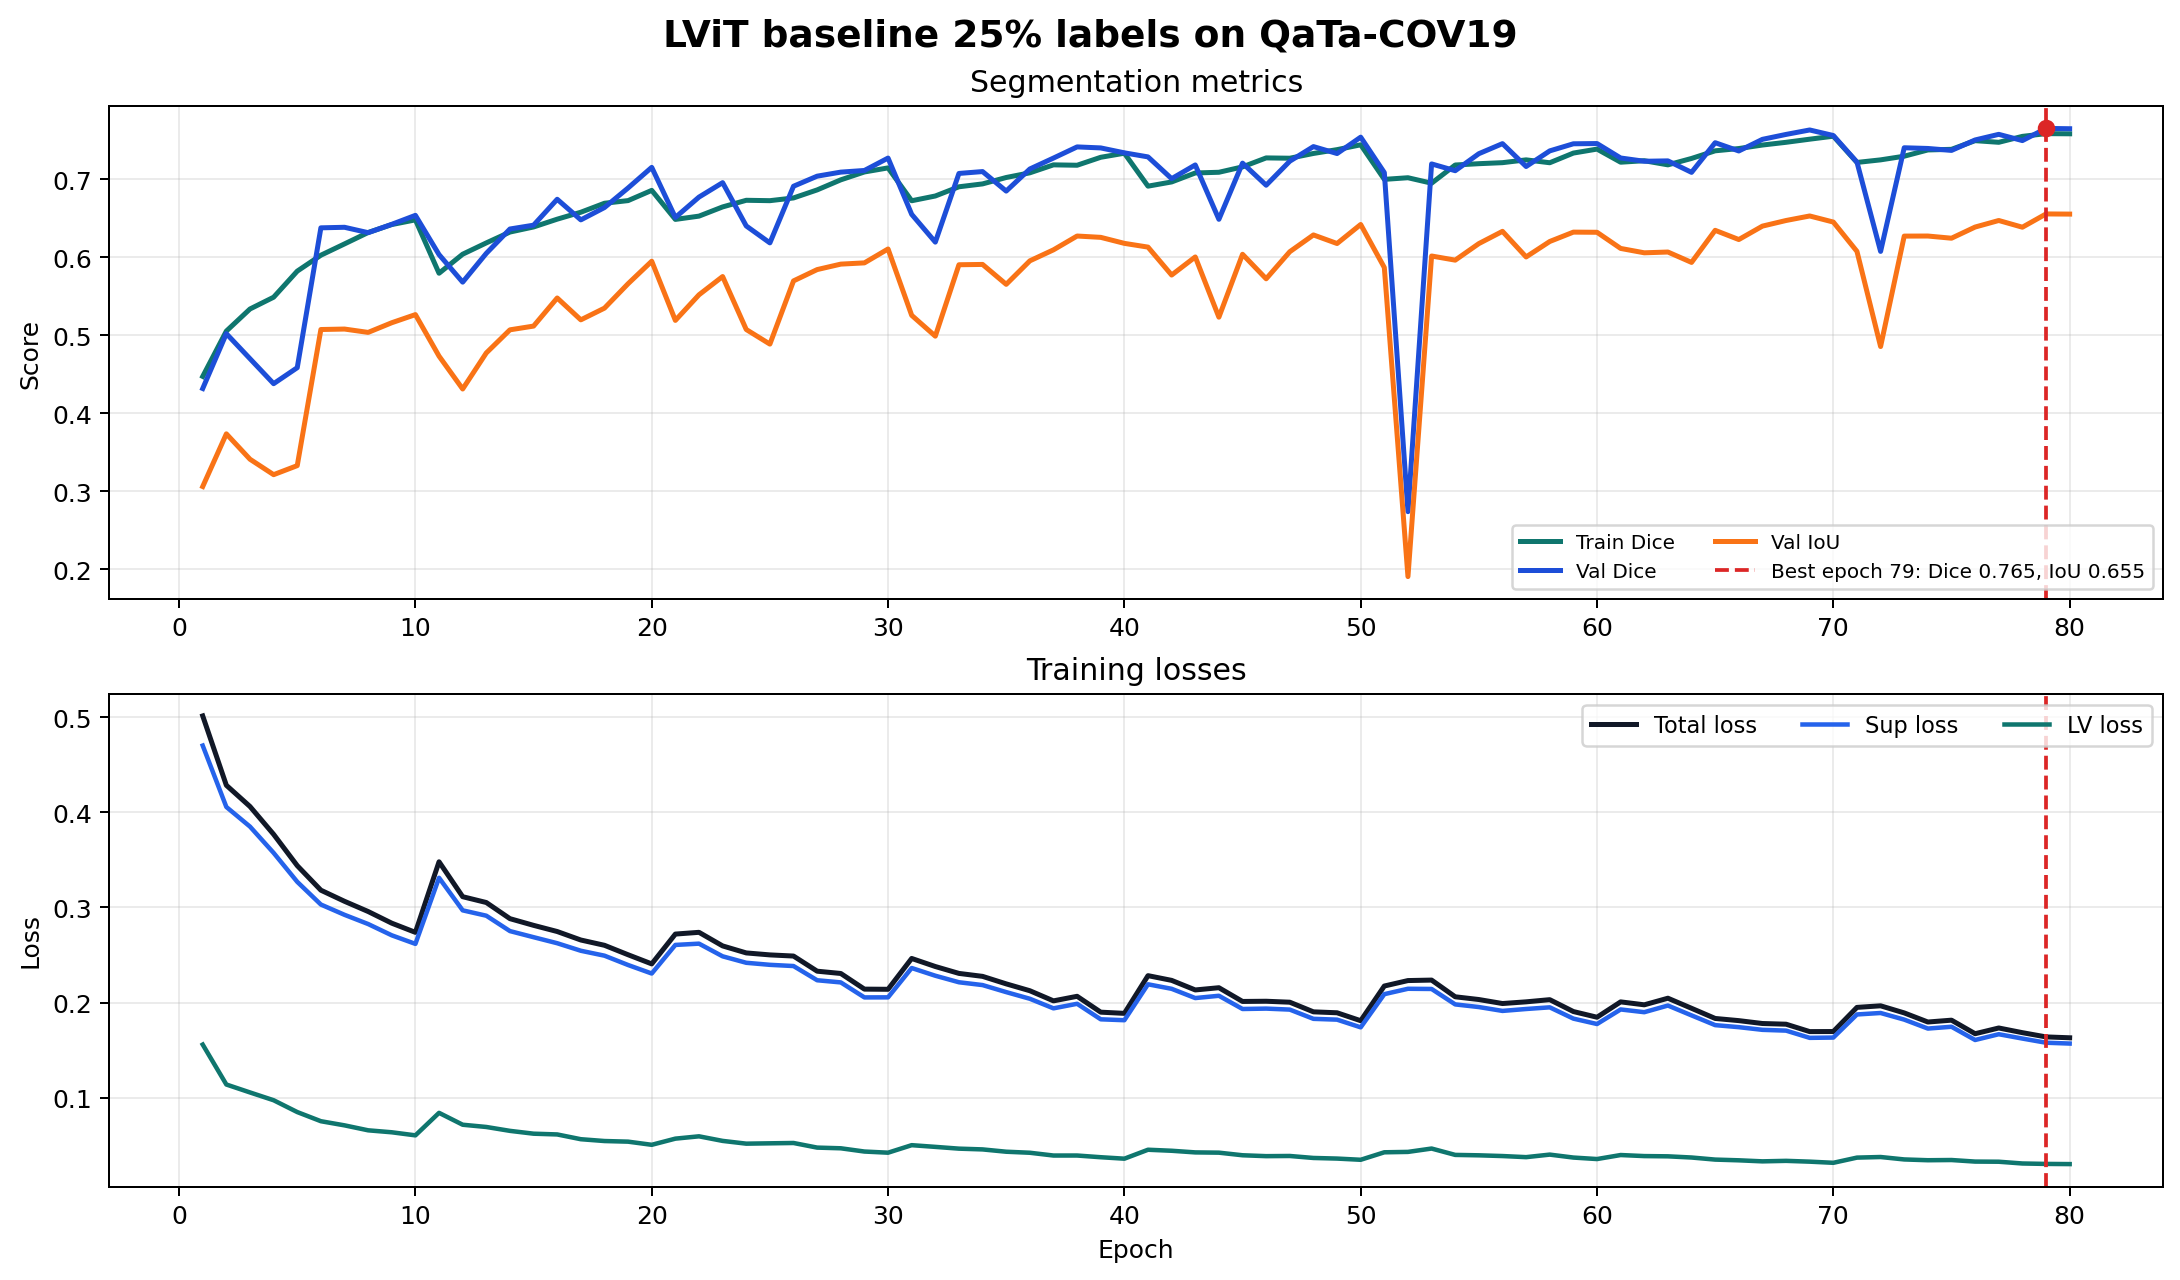
\includegraphics[width=0.96\textwidth]{figures/lvit_baseline_25pct_training_curves.png}
  \caption{Learning curve của LViT baseline 25\% nhãn trên QaTa-COV19. Đường metric cho thấy mô hình tăng nhanh ở giai đoạn đầu rồi dao động quanh vùng hội tụ; loss giảm dần và LV loss đóng vai trò tín hiệu bổ trợ nhỏ hơn supervised loss.}
  \label{fig:lvit-baseline-25-training-curves}
\end{figure}

Hình~\ref{fig:lvit-baseline-25-training-curves} cho thấy mô hình học được tín hiệu phân đoạn khá sớm: validation Dice tăng mạnh trong những epoch đầu, sau đó dao động quanh vùng 0.75--0.765. Epoch tốt nhất theo validation Dice là epoch 79 với Dice 0.765 và IoU 0.6554; epoch cuối đạt Dice 0.7646 và IoU 0.6552, gần như không suy giảm so với epoch tốt nhất. Điều này cho thấy baseline không bị sụp ở cuối quá trình học. Tuy nhiên, độ dao động validation cũng nói rằng học với 25\% nhãn vẫn nhạy: khi số mask thật ít, pseudo-label và văn bản loss giúp bổ sung tín hiệu nhưng không loại bỏ hoàn toàn nhiễu vùng biên.

\begin{figure}[H]
  \centering
  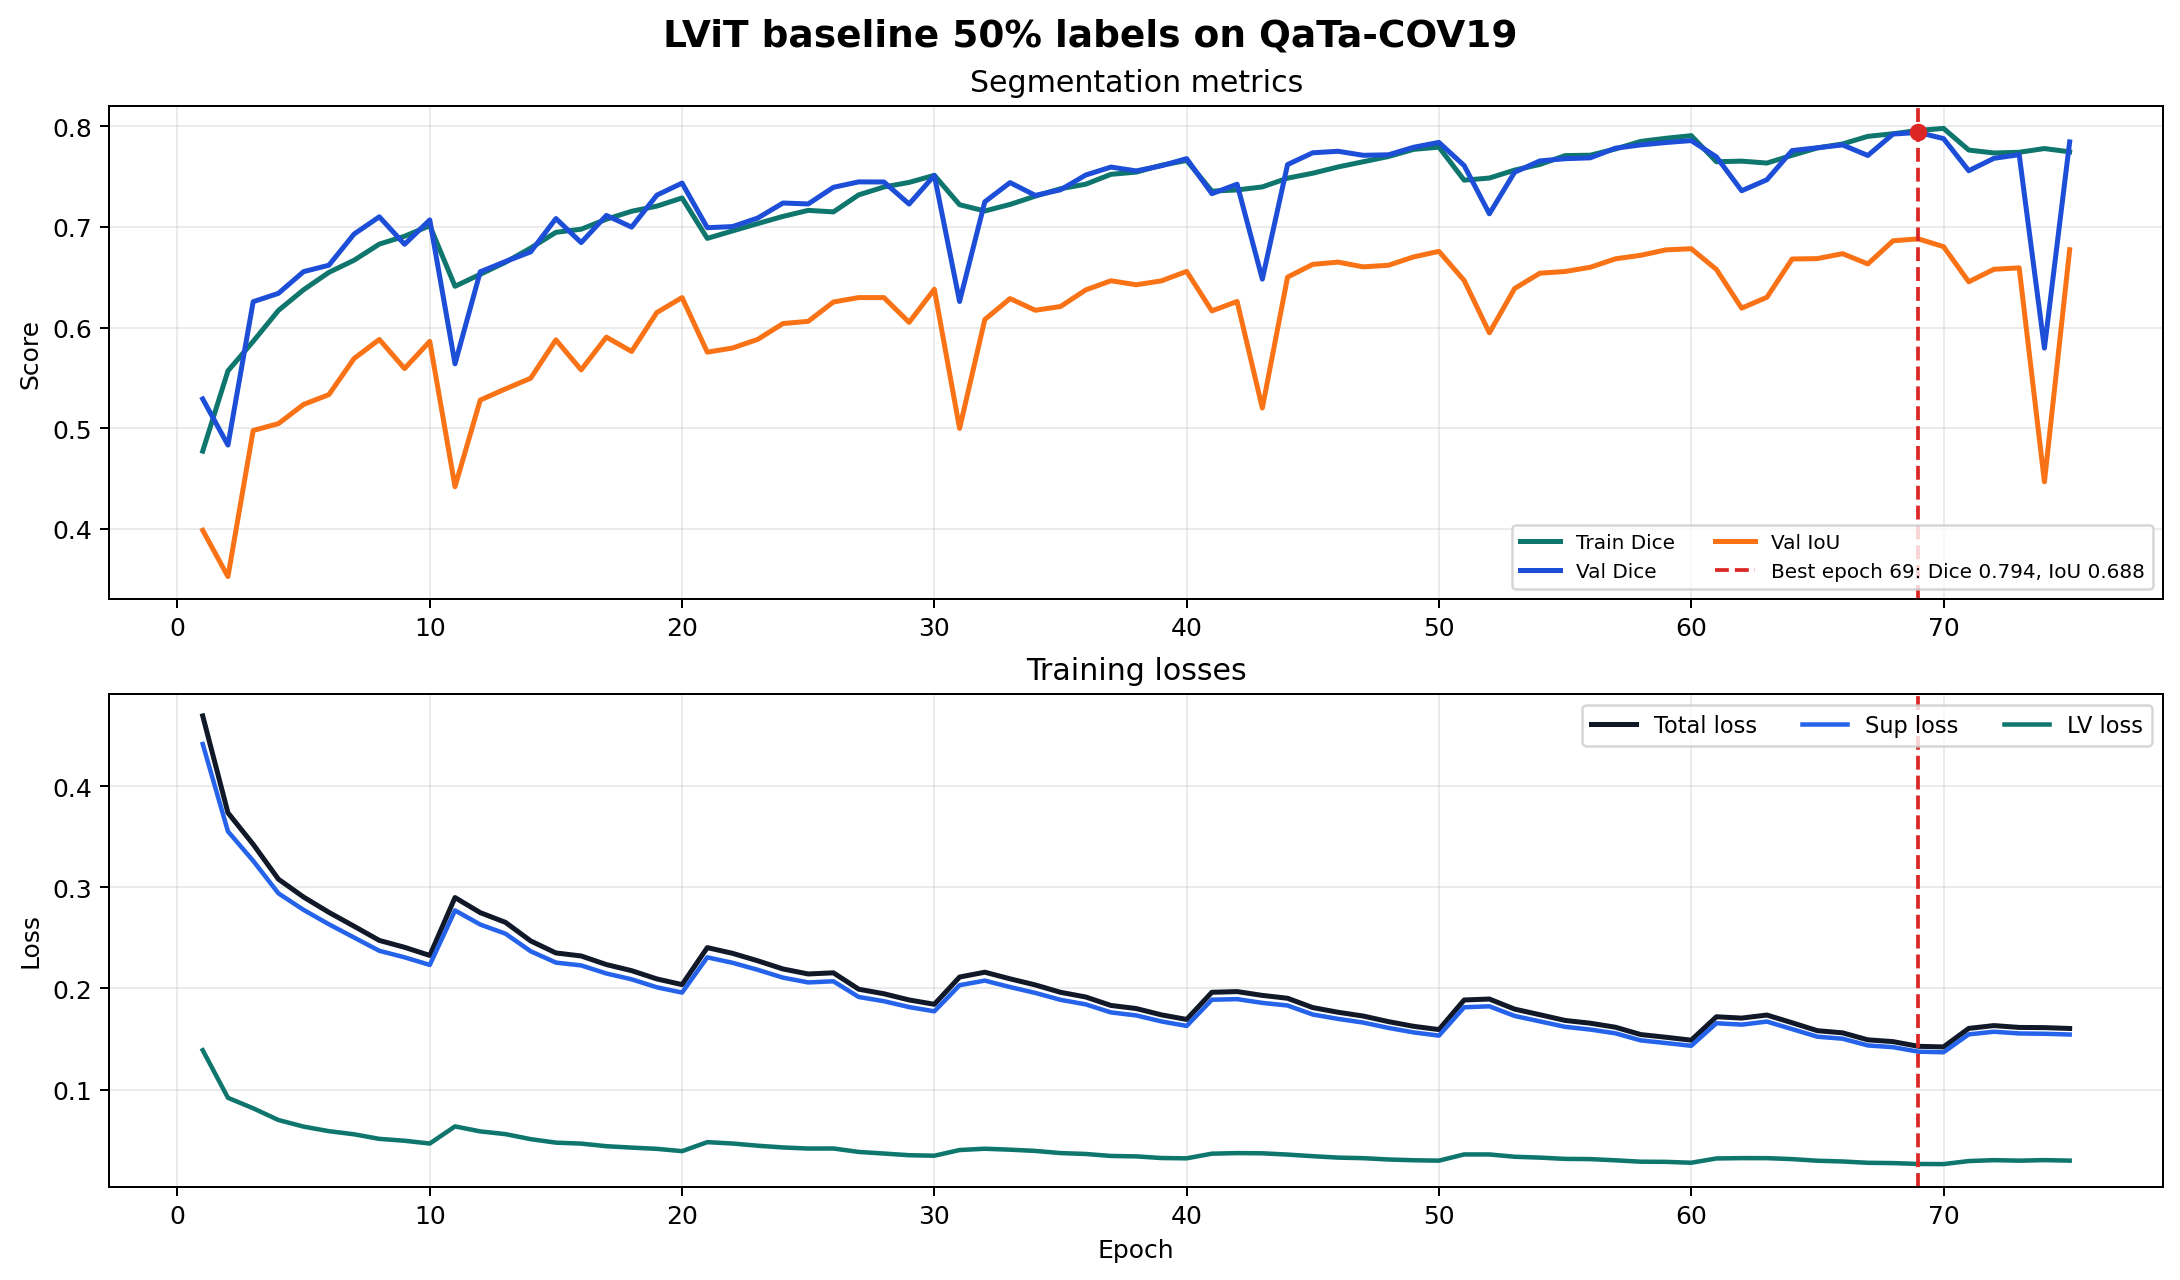
\includegraphics[width=0.96\textwidth]{figures/lvit_baseline_50pct_training_curves.png}
  \caption{Learning curve của LViT baseline 50\% nhãn trên QaTa-COV19. So với 25\% nhãn, validation Dice đạt mức cao hơn và tín hiệu supervised ổn định hơn nhờ số mẫu có mask thật tăng gấp đôi.}
  \label{fig:lvit-baseline-50-training-curves}
\end{figure}

Ở mức 50\% nhãn, Hình~\ref{fig:lvit-baseline-50-training-curves} cho thấy mô hình đạt validation Dice tốt nhất 0.7938 tại epoch 69, với IoU 0.6881. Epoch cuối đạt 0.7844 Dice và 0.6773 IoU, thấp hơn đỉnh tốt nhất nhưng vẫn cao hơn rõ so với mức 25\%. Một dao động mạnh xuất hiện gần cuối, cho thấy ngay cả khi tăng nhãn lên 50\%, huấn luyện bán giám sát vẫn nhạy với pseudo-label và vùng biên mờ. Tuy nhiên, mặt bằng metric đã được nâng lên, xác nhận vai trò nền tảng của ground truth chuyên gia.

\begin{figure}[H]
  \centering
  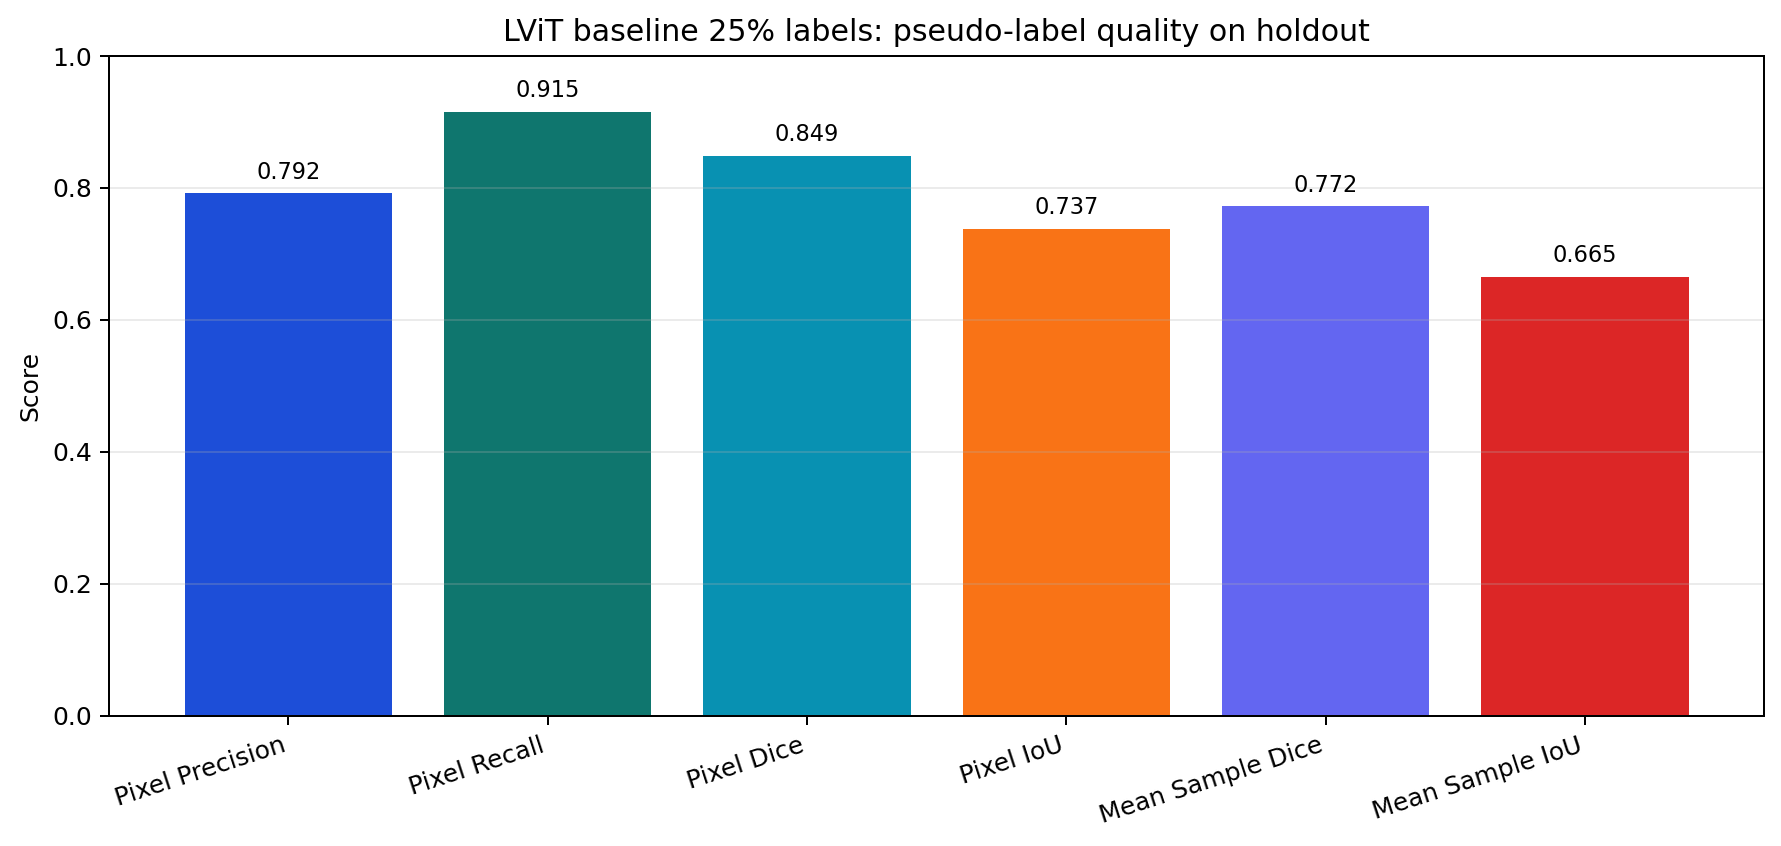
\includegraphics[width=0.86\textwidth]{figures/lvit_baseline_25pct_pseudo_holdout.png}
  \caption{Đánh giá pseudo-label của LViT baseline trên phần train chưa nhãn được giữ lại để đối sánh với ground truth.}
  \label{fig:lvit-baseline-25-pseudo-holdout}
\end{figure}

Chất lượng pseudo-label trong Hình~\ref{fig:lvit-baseline-25-pseudo-holdout} giúp giải thích vì sao LViT có thể học trong điều kiện ít nhãn. Trên phần holdout chưa nhãn, điểm ảnh Dice đạt 0.8489 và điểm ảnh IoU đạt 0.7374; recall cao 0.9150 cho thấy pseudo-label có xu hướng phủ được phần lớn vùng tổn thương. Tuy nhiên, khi tính trung bình theo từng mẫu, Dice giảm còn 0.7719 và IoU còn 0.6655. Khoảng cách giữa mức điểm ảnh và sample-level cho thấy pseudo-label không đồng đều giữa các ảnh: có ảnh dự đoán rất tốt, nhưng cũng có ảnh vùng mờ hoặc vùng nhỏ làm điểm từng mẫu giảm. Đây chính là lý do EPI và LV loss cần được xem là cơ chế kiểm soát chất lượng, không phải bảo đảm rằng mọi pseudo-label đều đúng.

\begin{figure}[H]
  \centering
  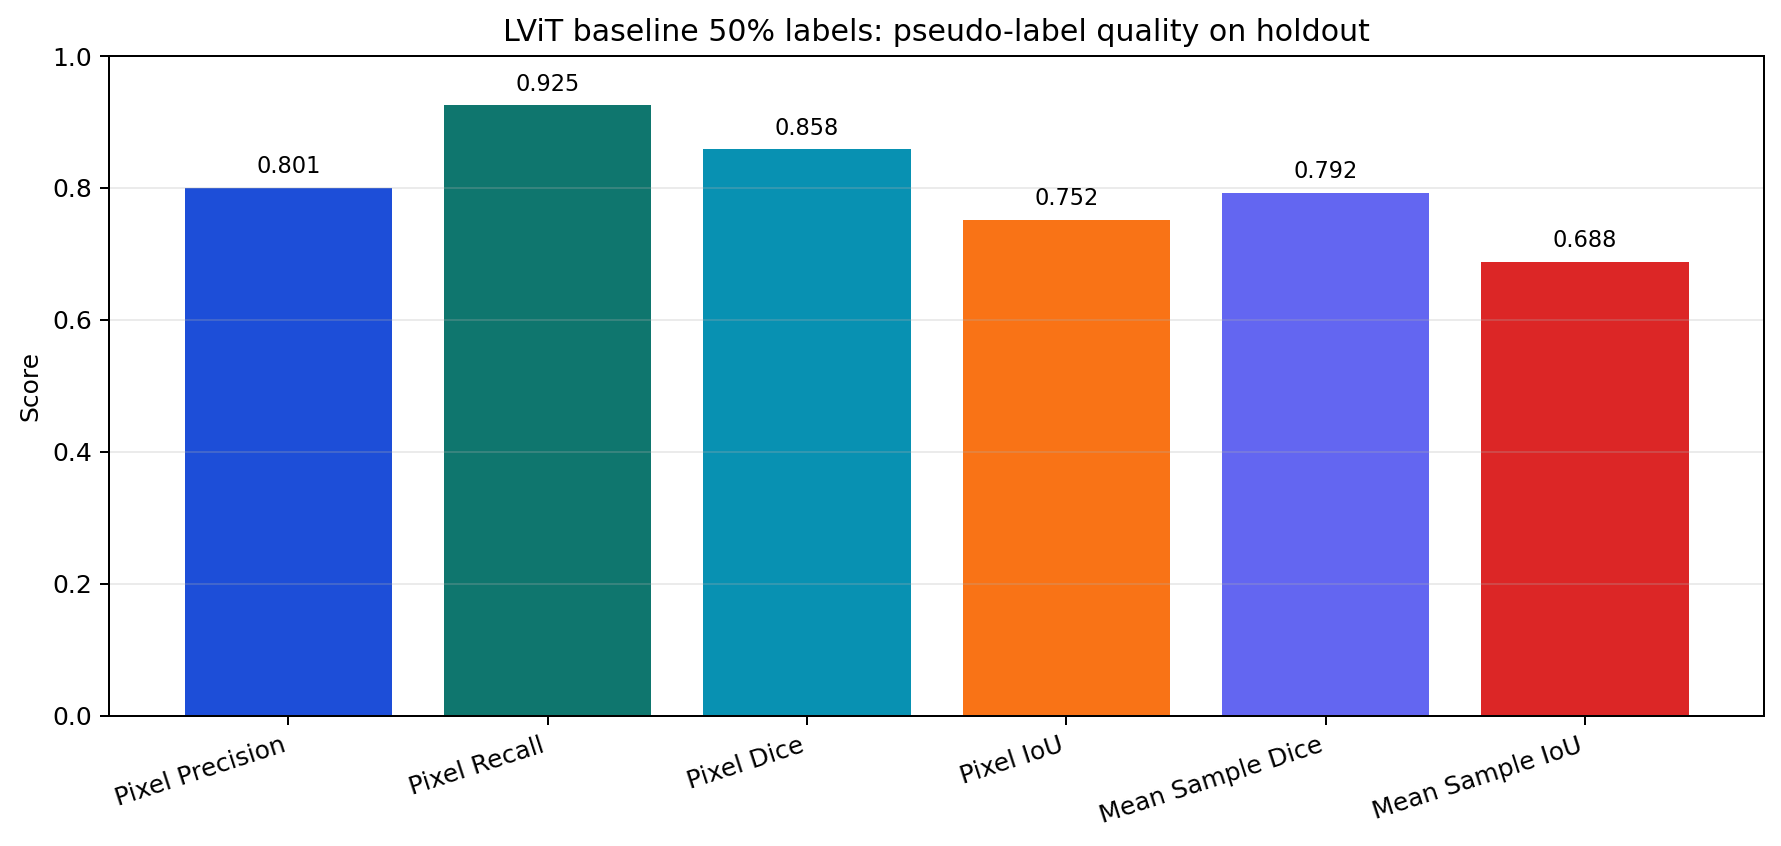
\includegraphics[width=0.86\textwidth]{figures/lvit_baseline_50pct_pseudo_holdout.png}
  \caption{Đánh giá pseudo-label của LViT baseline 50\% nhãn trên phần train chưa nhãn được giữ lại để đối sánh với ground truth.}
  \label{fig:lvit-baseline-50-pseudo-holdout}
\end{figure}

Khi tăng lên 50\% nhãn, pseudo-label holdout cũng cải thiện: điểm ảnh Dice đạt 0.8583, điểm ảnh IoU đạt 0.7517, mean sample Dice đạt 0.7923 và mean sample IoU đạt 0.6879. So với 25\% nhãn, cải thiện ở mean sample Dice khoảng 2.05 điểm phần trăm. Điều này quan trọng vì mean sample metric phản ánh chất lượng trên từng ảnh, không chỉ tổng số điểm ảnh. Nói cách khác, thêm mask thật không chỉ tăng metric test, mà còn làm pseudo-label bớt lệch giữa các mẫu.

\begin{figure}[H]
  \centering
  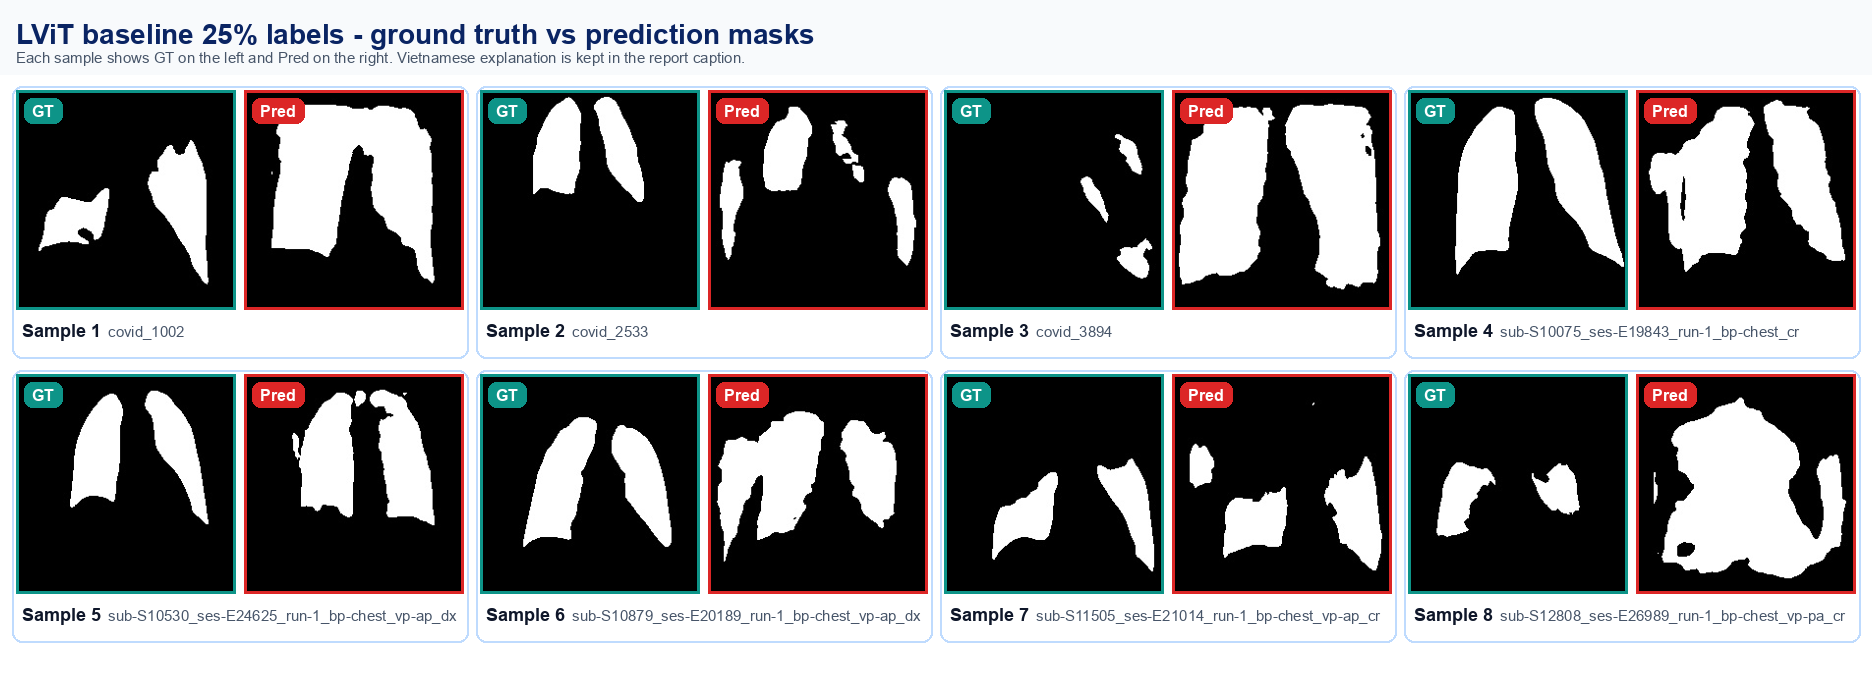
\includegraphics[width=0.98\textwidth]{figures/lvit_baseline_25pct_val_artifacts.png}
  \caption{Artifact trực quan từ LViT baseline 25\% nhãn trên validation: mỗi mẫu gồm mask thật và mask dự đoán.}
  \label{fig:lvit-baseline-25-val-artifacts}
\end{figure}

Artifact trực quan ở Hình~\ref{fig:lvit-baseline-25-val-artifacts} cho phép đọc kết quả sâu hơn bảng số. Nhìn chung, baseline đã học được vị trí tổn thương chính và có thể tạo mask ở các vùng mờ hai phổi. Tuy vậy, sai số thường nằm ở ba dạng. Dạng thứ nhất là \textit{dự đoán lan rộng}: mask dự đoán phủ quá rộng quanh vùng tổn thương, làm Dice còn chấp nhận được nhưng IoU bị phạt. Dạng thứ hai là \textit{bỏ sót cụm nhỏ}: các vùng foreground nhỏ hoặc mờ có thể không vượt ngưỡng. Dạng thứ ba là \textit{biên chưa sắc}: dự đoán bám được vùng bệnh nhưng ranh giới không trùng hoàn toàn với mask chuyên gia. Ba dạng sai số này khớp với EDA ở mục 4.3: QaTa-COV19 có biên tổn thương mờ và mask không đồng nhất, nên chỉ nhìn accuracy hoặc một vài ảnh đẹp sẽ không đủ.

\begin{figure}[H]
  \centering
  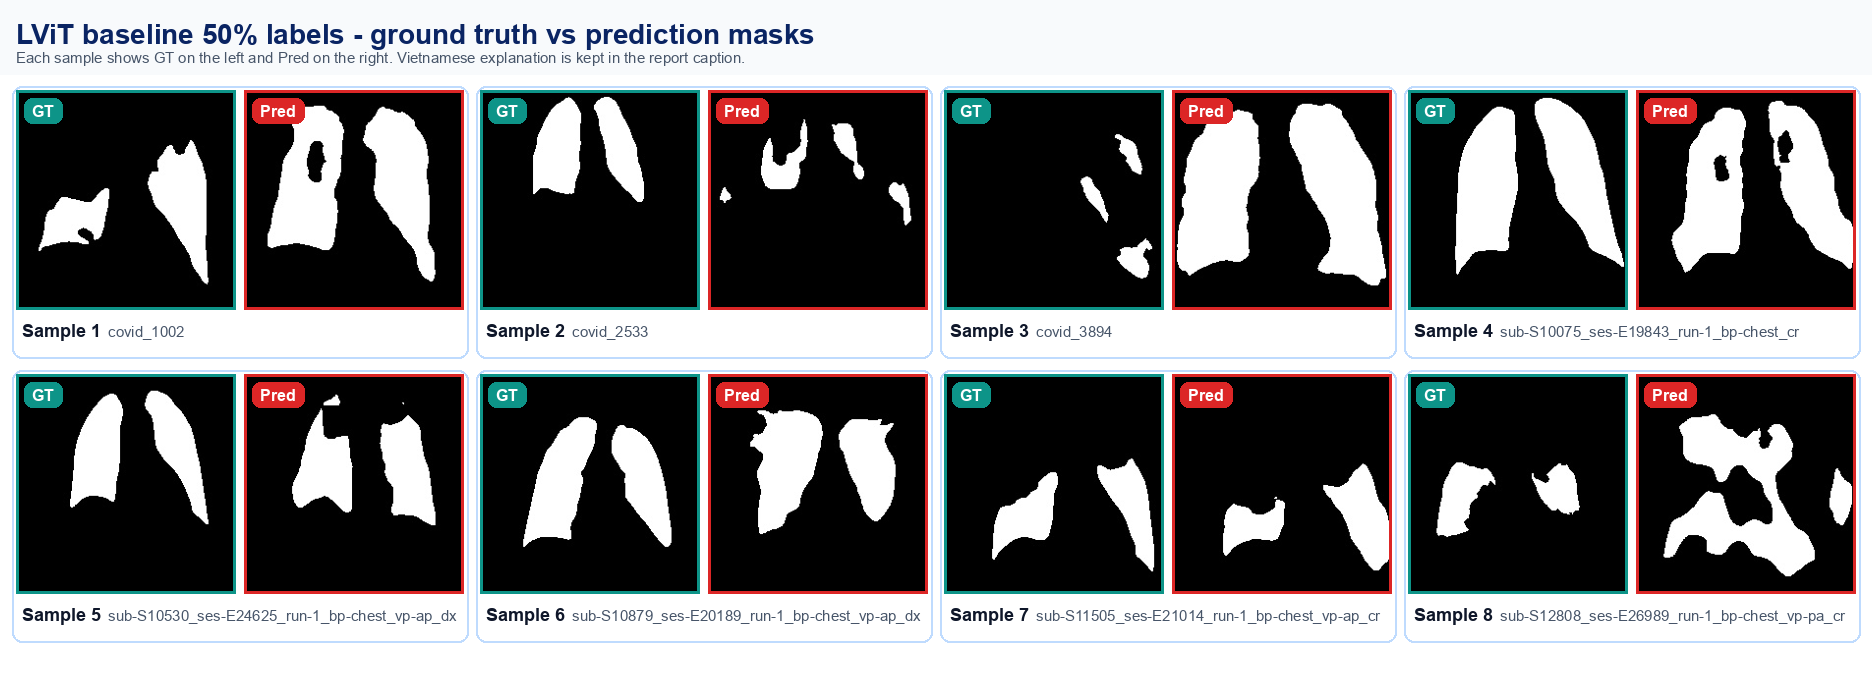
\includegraphics[width=0.98\textwidth]{figures/lvit_baseline_50pct_val_artifacts.png}
  \caption{Artifact trực quan từ LViT baseline 50\% nhãn trên validation: mỗi mẫu gồm mask thật và mask dự đoán.}
  \label{fig:lvit-baseline-50-val-artifacts}
\end{figure}

Artifact 50\% trong Hình~\ref{fig:lvit-baseline-50-val-artifacts} cho thấy dự đoán có xu hướng bám vùng tổn thương chính tốt hơn, nhưng ba loại lỗi của 25\% vẫn chưa biến mất hoàn toàn: biên vùng mờ chưa sắc, một số cụm nhỏ còn bị bỏ sót, và có trường hợp dự đoán lan rộng. Điều này dẫn tới một nhận xét quan trọng cho phần cải tiến: tăng nhãn giúp baseline mạnh hơn, nhưng không tự giải quyết hết bài toán hợp nhất ảnh--văn bản và kiểm soát pseudo-label. Vì vậy, cải tiến không nên chỉ được đánh giá ở một mức nhãn; cần nhìn cả 25\%, 50\% và 100\% để thấy cải tiến còn đóng góp khi baseline đã tốt hơn.

\begin{figure}[H]
  \centering
  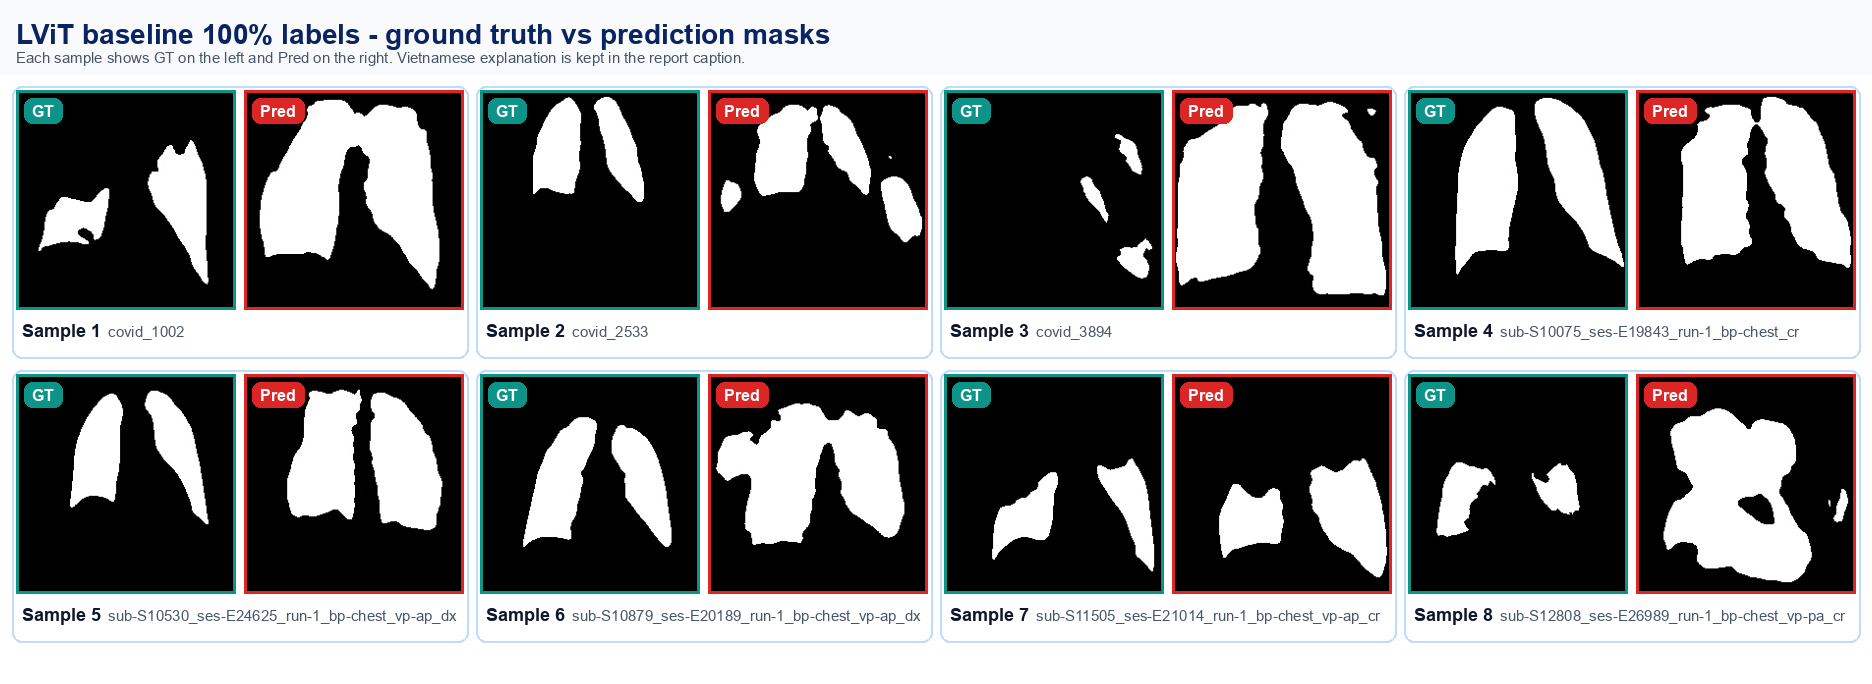
\includegraphics[width=0.98\textwidth]{figures/lvit_baseline_100pct_val_artifacts.png}
  \caption{Artifact trực quan từ LViT baseline 100\% nhãn trên validation: mỗi mẫu gồm mask thật và mask dự đoán.}
  \label{fig:lvit-baseline-100-val-artifacts}
\end{figure}

Artifact 100\% trong Hình~\ref{fig:lvit-baseline-100-val-artifacts} là mốc quan trọng để đọc giới hạn của LViT baseline khi đã dùng toàn bộ mask train. So với 25\% và 50\%, dự đoán thường đầy đủ hơn và ít phụ thuộc vào pseudo-label hơn, thể hiện qua test Dice 82.76. Tuy vậy, một số lỗi hình thái vẫn còn: vùng dự đoán có thể rộng hơn mask thật, rìa mask chưa sắc ở vùng tổn thương mờ, và các vùng nhỏ vẫn có nguy cơ bị nhập vào vùng lớn hơn. Điều này cho thấy ngay cả khi có đủ nhãn, bài toán không chỉ là thiếu dữ liệu; nó còn phụ thuộc vào cách mô hình giữ chi tiết không gian, học ngữ cảnh xa và kết hợp văn bản với ảnh.

\FloatBarrier

\textbf{Kết quả chính của QaTaLViT cải tiến.} Sau khi đã có baseline chạy lại để đọc hành vi của LViT, phần cải tiến được đánh giá trên cùng hướng câu hỏi: khi thay đổi biểu diễn văn bản, fusion, prior và cơ chế kiểm soát nhãn giả, kết quả có tăng không và tăng ở điều kiện nào. Kết quả chính ở Bảng~\ref{tab:qatalvit-main-results} cho thấy QaTaLViT cải thiện rõ ở cả ba mức nhãn. Mức tăng lớn nhất xuất hiện ở 25\% và 50\% nhãn, đúng với động lực ban đầu của LViT: khi mặt nạ chuyên gia ít, mô hình có lợi hơn từ văn bản chú thích, prior và pseudo-label. Ở mức 100\% nhãn, mức tăng nhỏ hơn nhưng vẫn dương, cho thấy phần cải tiến không chỉ là cơ chế bù nhãn thiếu mà còn có thể cải thiện biểu diễn ảnh--văn bản khi có đủ mask.

\textbf{Ablation chính.}

Bảng ablation chính trên QaTa-COV19 được thiết kế để trả lời câu hỏi: mỗi nhóm cải tiến đóng góp thế nào khi tỉ lệ nhãn thay đổi. Các tên B0, I1, I2, I3, I4 và I5 chỉ là mã cấu hình để bảng gọn hơn; nếu không giải thích, các tên này không có ý nghĩa học thuật. Vì vậy, trước khi đọc điểm số, cần hiểu mỗi dòng là một thay đổi cụ thể so với pipeline đã mô tả ở mục kế hoạch thực nghiệm. Baseline là LViT chạy lại theo recipe gốc. B0 là bước khởi đầu khi chuyển sang khung huấn luyện cải tiến nhưng văn bản/prompt chưa được chuẩn hóa tốt. I1 thêm chuẩn hóa prompt. I2--I5 lần lượt kiểm tra các nhóm thay đổi về bộ mã hóa văn bản, fusion ảnh--văn bản, prior/skip đặc trưng và kiểm soát pseudo-label/loss. Dòng QaTaLViT là recipe cuối, tức là cấu hình đã gom các thành phần hoạt động ổn định nhất để báo cáo kết quả chính.

\begin{table}[H]
  \centering
  \caption{Chú giải các cấu hình ablation QaTaLViT. Các dòng I2--I5 là ablation theo nhóm thay đổi, không phải chỉ thay đúng một dòng code.}
  \label{tab:qatalvit-ablation-legend}
  \scriptsize
  \renewcommand{\arraystretch}{1.12}
  \setlength{\tabcolsep}{4pt}
  \begin{tabularx}{\textwidth}{@{}p{0.14\textwidth} Y Y@{}}
    \toprule
    Ký hiệu & Thay đổi chính so với cấu hình trước/baseline & Ý nghĩa cần kiểm tra \\
    \midrule
    Baseline (LViT) & Dùng LViT gốc/chạy lại: ảnh + văn bản chú thích, Double-U, LV Fusion, PLAM, EPI/LV loss theo tinh thần paper & Là mốc để biết cải tiến có thật sự hơn LViT hay không \\
    B0 & Chuyển sang khung huấn luyện/cải tiến ban đầu nhưng văn bản prompt còn thô, chưa chuẩn hóa ngữ nghĩa và hình thức & Kiểm tra rủi ro khi thêm pipeline mới nhưng văn bản còn nhiễu \\
    I1 & Thêm prompt normalization: chuẩn hóa cách diễn đạt vị trí, số vùng, trái/phải và các cụm mô tả lặp lại & Đo tác động riêng của việc làm văn bản nhất quán hơn \\
    I2 & Thêm biểu diễn văn bản y sinh và tương tác ảnh--văn bản mạnh hơn, ví dụ BiomedBERT/cache embedding và bottleneck/cross-modal fusion & Kiểm tra liệu bộ mã hóa y sinh và fusion rõ hơn có giúp mô hình định vị tổn thương tốt hơn \\
    I3 & Bổ sung prior không gian từ văn bản hoặc điều chỉnh cách đưa văn bản vào các tầng thấp/cao của mạng & Kiểm tra văn bản có thể đóng vai trò gợi ý vị trí mềm, thay vì chỉ là vector ngữ nghĩa toàn cục \\
    I4 & Tăng cường nhánh bộ giải mã/skip đặc trưng bằng adapter hoặc cơ chế lọc đặc trưng theo văn bản & Kiểm tra việc kiểm soát skip connection có giảm truyền nhiễu nền và cải thiện biên mask không \\
    I5 & Tập trung vào nhãn giả và loss: confidence mask, consistency, boundary/prototype alignment hoặc fusion pseudo-label & Kiểm tra pseudo-label giúp học thêm hay làm lan truyền sai số khi mask thật ít \\
    QaTaLViT & Recipe cuối: gom prompt normalization, bộ mã hóa văn bản phù hợp, fusion/prior/skip ổn định và cơ chế kiểm soát pseudo-label đã chọn & Đánh giá cấu hình hoàn chỉnh thay vì một module đơn lẻ \\
    \bottomrule
  \end{tabularx}
\end{table}
\FloatBarrier

\begin{table}[H]
  \centering
  \caption{Ablation chính trên QaTa-COV19. Giá trị là test Dice/IoU, đơn vị phần trăm.}
  \label{tab:qatalvit-ablation-main}
  \scriptsize
  \renewcommand{\arraystretch}{1.12}
  \setlength{\tabcolsep}{4pt}
  \begin{tabularx}{\textwidth}{@{}l Y Y Y@{}}
    \toprule
    Phương pháp & 25\% nhãn & 50\% nhãn & 100\% nhãn \\
    \midrule
    Baseline (LViT) & 78.42 / 68.43 & 80.32 / 70.60 & 82.76 / 73.78 \\
    B0 & 77.49 / 67.19 & 79.54 / 69.71 & -- \\
    I1 & 78.46 / 68.23 & 80.89 / 71.54 & 82.84 / 74.14 \\
    I2 & 80.45 / 71.04 & 82.61 / 73.65 & 83.69 / 74.85 \\
    I3 & 78.96 / 69.22 & 82.61 / 73.65 & 83.05 / 74.45 \\
    I4 & 81.37 / 72.10 & 82.51 / 73.54 & 83.75 / 75.03 \\
    I5 & 80.24 / 70.57 & 82.94 / 74.10 & 83.67 / 74.97 \\
    QaTaLViT & \textbf{82.22 / 73.35} & \textbf{84.03 / 75.62} & \textbf{85.28 / 77.25} \\
    \bottomrule
  \end{tabularx}
\end{table}
\FloatBarrier

Kết quả cho thấy ba điểm. Thứ nhất, B0 thấp hơn baseline, nghĩa là chỉ chuyển sang pipeline mới mà văn bản chưa chuẩn hóa hoặc chưa kiểm soát tốt có thể làm mô hình kém hơn. Điều này rất quan trọng vì nó nhắc lại nguyên tắc của LViT: văn bản hữu ích nhưng văn bản nhiễu hoặc không nhất quán có thể gây hại. Thứ hai, I1 cải thiện so với B0, đặc biệt ở 50\% nhãn, cho thấy chuẩn hóa prompt giúp giảm nhiễu ngôn ngữ trước khi bàn đến bộ mã hóa mạnh hơn. Thứ ba, I2--I5 đều vượt baseline ở nhiều mức, nhưng mỗi dòng mạnh ở một khía cạnh khác nhau: có dòng lợi ở 25\% nhãn do pseudo-label/prior tốt hơn, có dòng lợi ở 50\% do fusion/bộ mã hóa văn bản ổn định hơn, và có dòng lợi ở 100\% do bộ giải mã/skip đặc trưng giữ biên tốt hơn. Không một biến thể đơn lẻ nào thắng ổn định cả ba tỉ lệ nhãn như QaTaLViT cuối. Vì vậy, recipe cuối nên được hiểu là tổ hợp có kiểm soát, không phải một mẹo đơn độc.

Ở 25\% nhãn, mức tăng của QaTaLViT là lớn nhất. Đây là dấu hiệu hợp lý: khi mask ít, mô hình hưởng lợi nhiều hơn từ bộ mã hóa văn bản, prior và pseudo-label ổn định. Ở 100\% nhãn, mức tăng nhỏ hơn nhưng vẫn tồn tại, cho thấy cải tiến không chỉ bù cho thiếu nhãn mà còn làm biểu diễn ảnh--văn bản tốt hơn khi có đủ mask.

\begin{figure}[H]
  \centering
  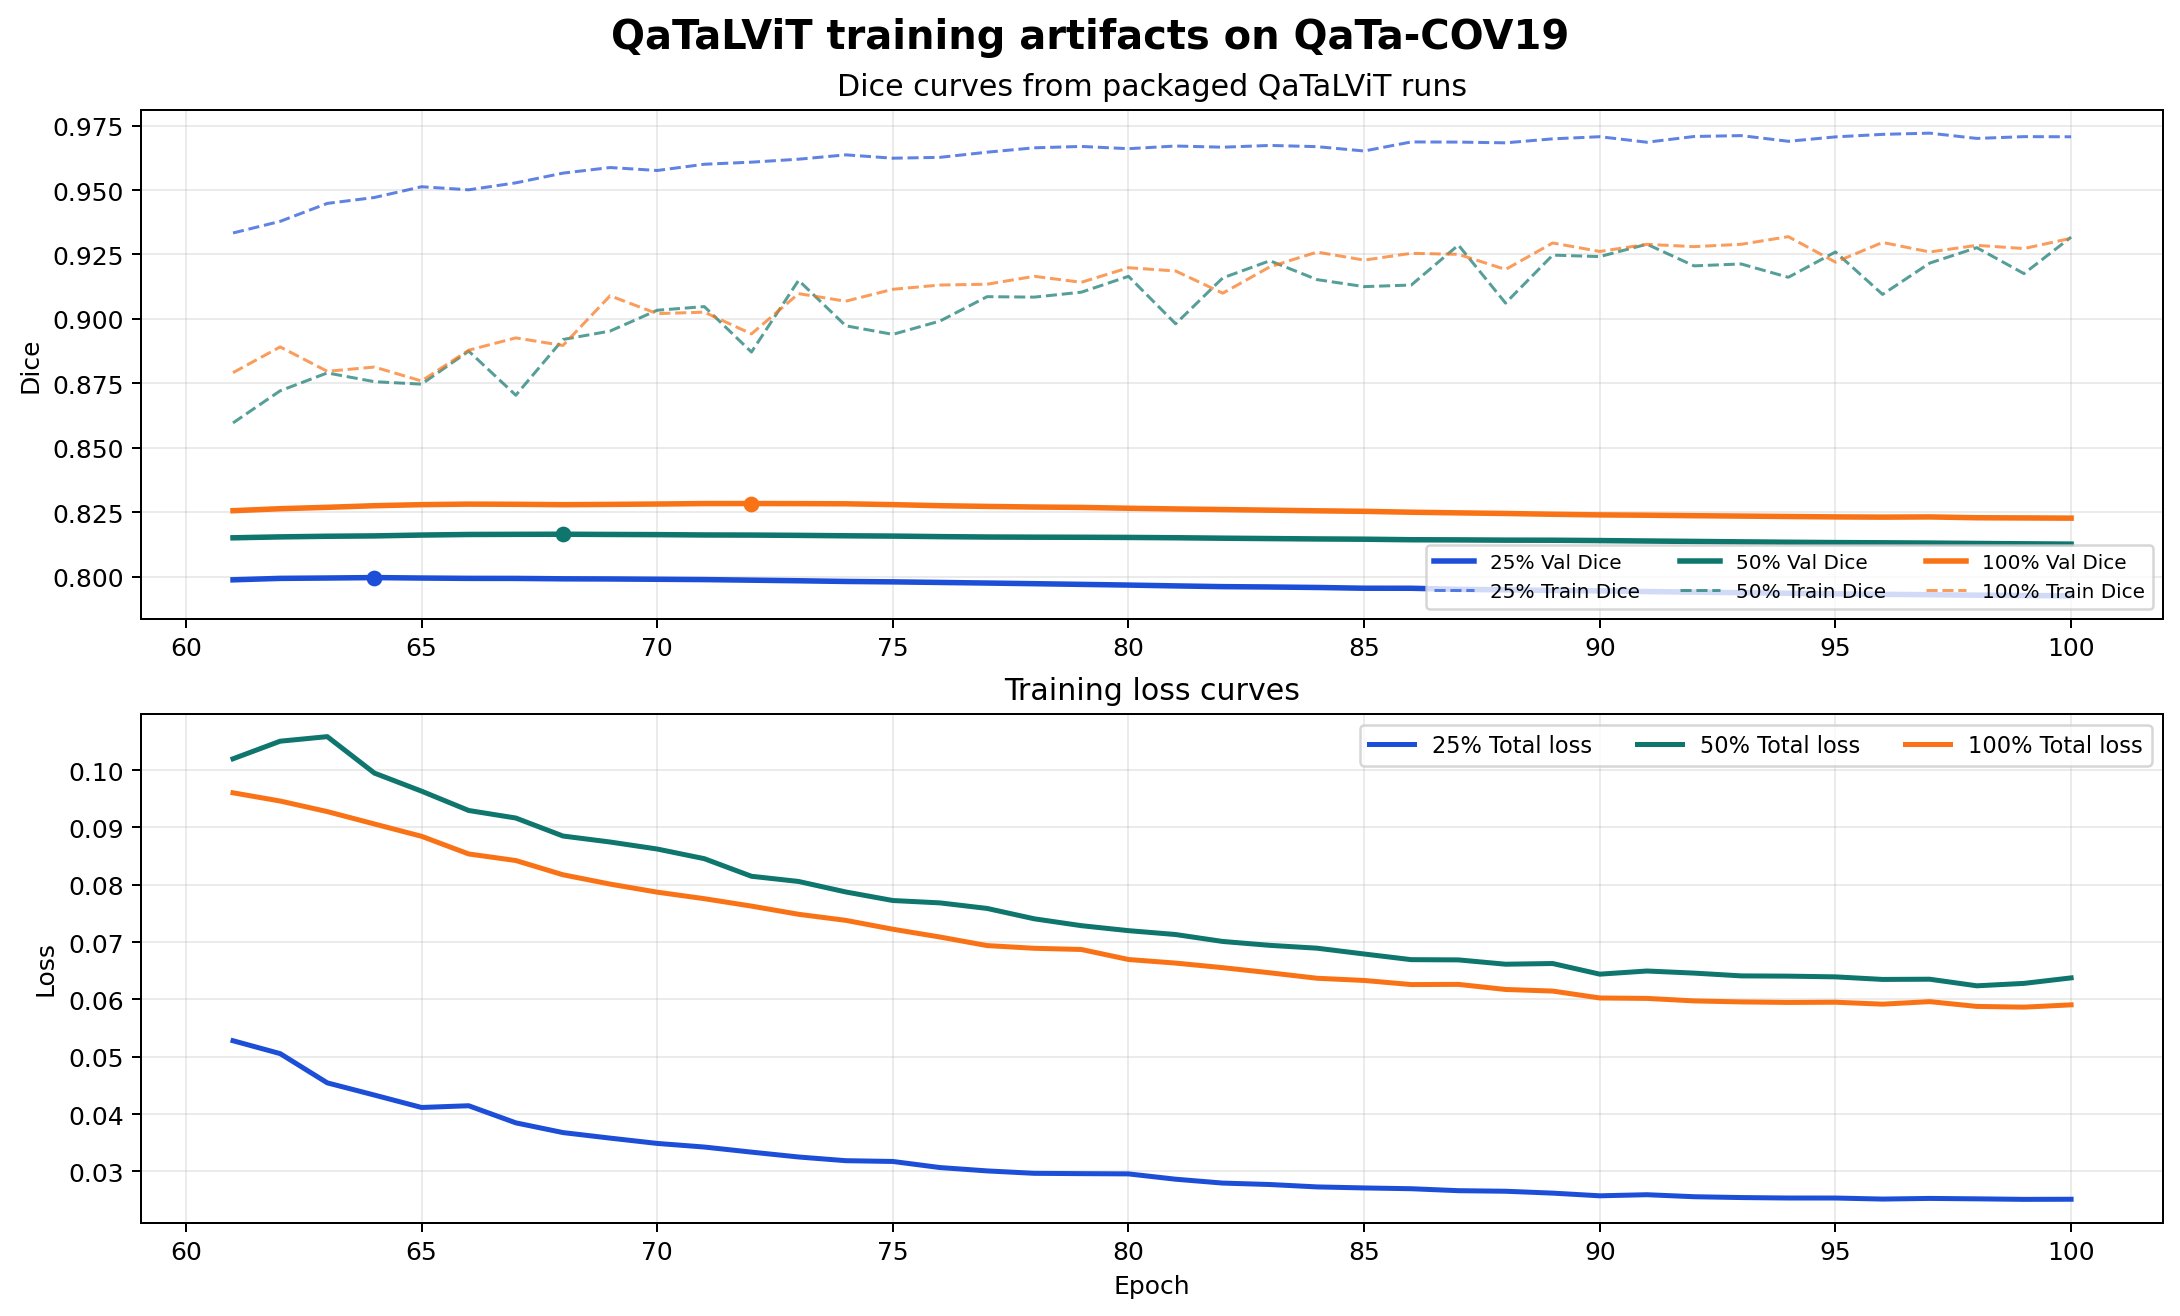
\includegraphics[width=0.96\textwidth]{figures/qatalvit_training_artifacts.png}
  \caption{Artifact huấn luyện của QaTaLViT trên QaTa-COV19 ở ba mức nhãn. Đường Dice validation cho thấy mô hình cải tiến duy trì mức validation cao hơn khi tỉ lệ nhãn tăng; đường loss giảm dần cho thấy quá trình fine-tune ổn định ở các epoch cuối.}
  \label{fig:qatalvit-training-artifacts}
\end{figure}

Hình~\ref{fig:qatalvit-training-artifacts} bổ sung cách đọc kết quả ngoài bảng Dice/IoU cuối. Ở cả ba mức nhãn, loss giảm dần trong giai đoạn cuối, nghĩa là quá trình tối ưu không chỉ tạo ra một điểm số đơn lẻ mà có xu hướng hội tụ. Đường train Dice cao hơn validation Dice, đặc biệt ở mức 25\%, phản ánh khoảng cách giữa khả năng khớp tập train và khả năng tổng quát. Khi tăng từ 25\% lên 50\% rồi 100\% nhãn, validation Dice tăng theo, phù hợp với trực giác rằng mask thật vẫn là tín hiệu mạnh nhất. Tuy vậy, mức tăng của QaTaLViT so với LViT baseline ở 25\% và 50\% vẫn lớn, cho thấy phần cải tiến có ý nghĩa rõ nhất khi dữ liệu gán nhãn còn hạn chế.

\begin{figure}[H]
  \centering
  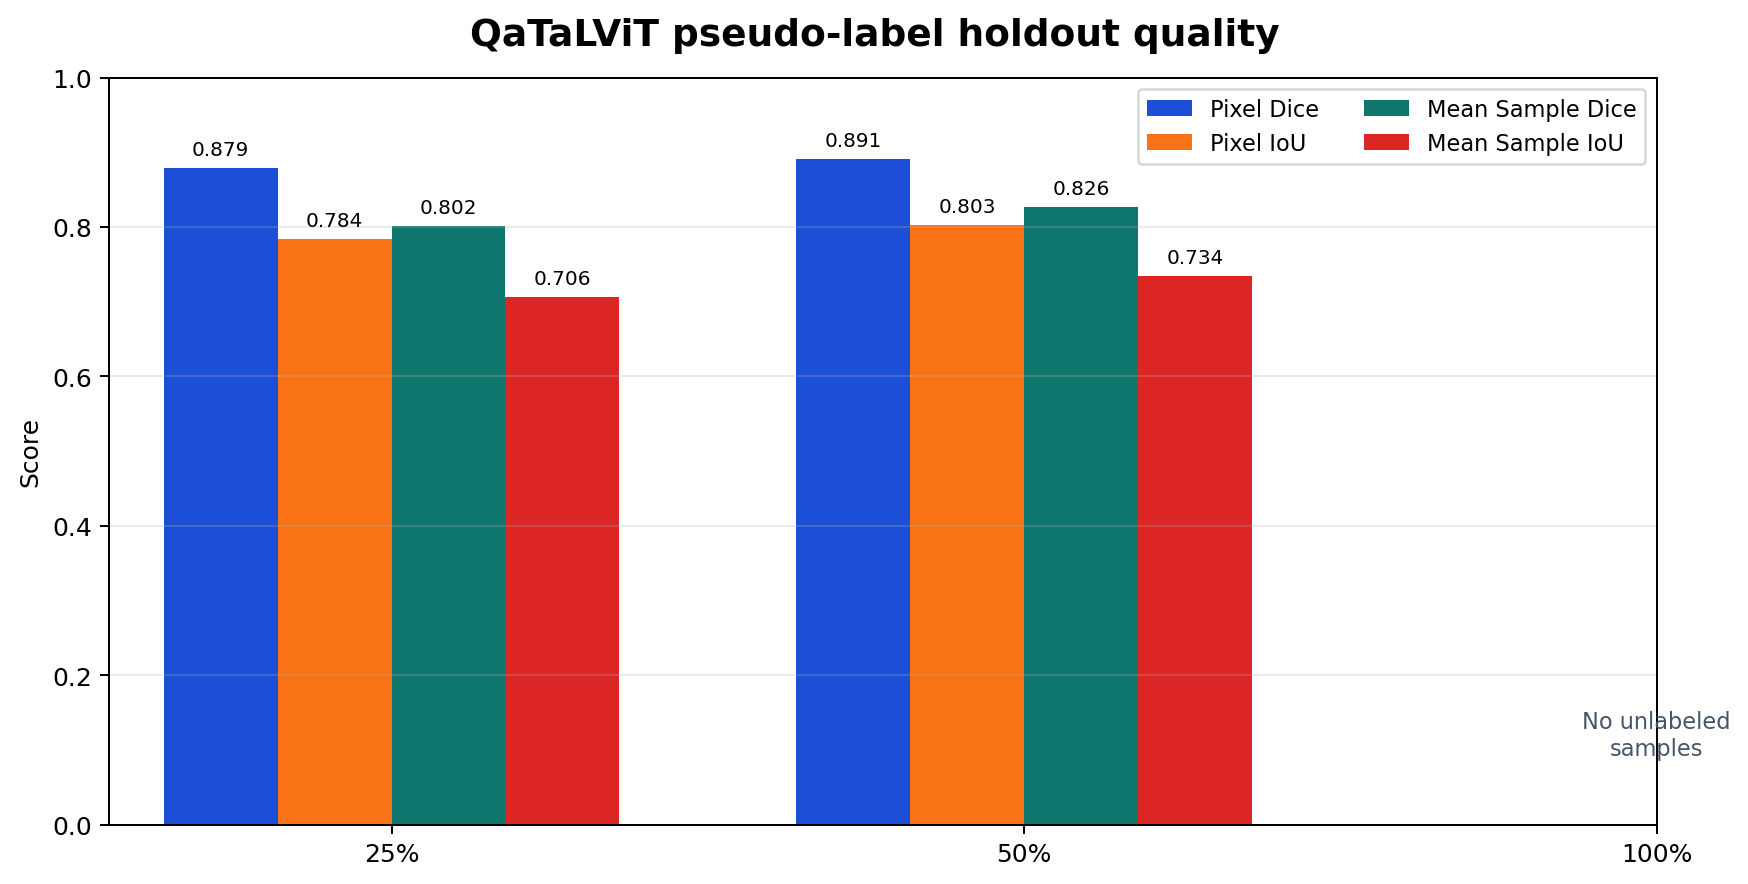
\includegraphics[width=0.88\textwidth]{figures/qatalvit_pseudo_holdout.png}
  \caption{Chất lượng pseudo-label của QaTaLViT trên phần dữ liệu chưa nhãn ở mức 25\% và 50\% nhãn. Ở mức 100\% không còn mẫu chưa nhãn nên không có pseudo-label holdout.}
  \label{fig:qatalvit-pseudo-holdout}
\end{figure}

Hình~\ref{fig:qatalvit-pseudo-holdout} cho thấy pseudo-label của QaTaLViT có chất lượng khá cao trên phần dữ liệu chưa nhãn. Ở 25\% nhãn, điểm ảnh Dice của pseudo-label đạt khoảng 0.879 và mean-sample Dice đạt khoảng 0.802. Khi tăng lên 50\% nhãn, điểm ảnh Dice tăng lên khoảng 0.891 và mean-sample Dice tăng lên khoảng 0.826. Sự tăng này rất quan trọng: nó cho thấy khi mô hình được neo bởi nhiều mask thật hơn, pseudo-label không chỉ tốt hơn ở tổng điểm ảnh mà còn ổn định hơn theo từng ảnh. Điều này củng cố vai trò của EPI/LV loss và cơ chế kiểm soát nhãn giả trong QaTaLViT: pseudo-label không được xem là ground truth, mà là tín hiệu tạm cần được lọc và kiểm soát.

\FloatBarrier

\begin{table}[H]
  \centering
  \caption{So sánh LViT baseline chạy lại và QaTaLViT cải tiến theo nhiều loại artifact trên QaTa-COV19.}
  \label{tab:lvit-vs-qatalvit-artifacts}
  \small
  \renewcommand{\arraystretch}{1.16}
  \setlength{\tabcolsep}{4pt}
  \begin{tabularx}{\textwidth}{@{}L Y Y@{}}
    \toprule
    Khía cạnh so sánh & LViT baseline chạy lại & QaTaLViT cải tiến \\
    \midrule
    Metric test & 25\%: 78.42 / 68.43; 50\%: 80.32 / 70.60; 100\%: 82.76 / 73.78 & 25\%: 82.22 / 73.35; 50\%: 84.03 / 75.62; 100\%: 85.28 / 77.25 \\
    Learning behavior & 25\% đạt best val Dice 0.765; 50\% đạt 0.7938; 100\% đạt validation Dice 81.21 theo metric tổng hợp & Kết quả ablation cho thấy cải tiến ổn định hơn khi kết hợp nhiều thành phần, không phụ thuộc một thay đổi đơn lẻ \\
    Pseudo-label & Mean sample Dice tăng từ 0.7719 ở 25\% lên 0.7923 ở 50\%, nhưng vẫn thấp hơn điểm ảnh Dice & Cải tiến tập trung vào kiểm soát pseudo-label bằng prior, fusion và loss để giảm rủi ro học theo nhãn giả nhiễu \\
    Artifact trực quan & 25\%, 50\% và 100\% đều có GT/Pred validation; tăng nhãn làm dự đoán đầy đủ hơn nhưng vẫn còn lan rộng, bỏ sót cụm nhỏ và biên chưa sắc & Cần được đọc qua tăng Dice/IoU và ablation; mục tiêu là giảm false positive/false negative ở vùng mờ hơn là chỉ tăng accuracy \\
    Ý nghĩa & Xác nhận LViT hưởng lợi khi tăng mask thật, đồng thời vẫn cần văn bản/pseudo-label trong vùng ít nhãn & Cho thấy pipeline ảnh--văn bản còn dư địa cải thiện khi chuẩn hóa văn bản, tăng tương tác ảnh--văn bản và kiểm soát nhãn giả tốt hơn \\
    \bottomrule
  \end{tabularx}
\end{table}
\FloatBarrier

Bảng~\ref{tab:lvit-vs-qatalvit-artifacts} nhấn mạnh rằng so sánh không chỉ dựa trên một dòng Dice/IoU. LViT baseline cho ta thấy quá trình học, chất lượng pseudo-label và hình dạng lỗi dự đoán; QaTaLViT cải tiến cần được đọc như lời đáp cho các lỗi đó. Nếu baseline đã phủ được vùng tổn thương nhưng còn lan rộng hoặc bỏ sót cụm nhỏ, thì cải tiến phải hướng đến biểu diễn không gian tốt hơn, fusion ảnh--văn bản rõ hơn và pseudo-label ổn định hơn. Mức tăng từ 78.42/68.43 lên 82.22/73.35 ở 25\% nhãn, từ 80.32/70.60 lên 84.03/75.62 ở 50\% nhãn, và từ 82.76/73.78 lên 85.28/77.25 ở 100\% nhãn vì vậy có ý nghĩa hơn một phép cộng điểm số: nó cho thấy cải tiến vẫn đánh đúng vùng yếu của LViT ngay cả khi lượng mask thật đã tăng.

\FloatBarrier

\textbf{Ablation biểu diễn văn bản.}

Vì LViT là mô hình ảnh--văn bản, bộ mã hóa văn bản là một điểm ablation quan trọng. Bảng dưới tách riêng ba mức: biểu diễn văn bản kiểu LViT/prompt chưa chuẩn hóa, prompt đã chuẩn hóa, pretrained BiomedBERT và NoBERT học từ đầu bằng embedding + BiGRU. Mục tiêu không phải chứng minh BiomedBERT luôn tốt trong mọi tình huống, mà xem văn bản y sinh pretrained có đáng giá so với bộ mã hóa nhẹ học từ dữ liệu đích hay không.

\begin{table}[H]
  \centering
  \caption{Ablation biểu diễn văn bản trên QaTa-COV19 50\%. Giá trị là test Dice/IoU, đơn vị phần trăm.}
  \label{tab:văn bản-bộ mã hóa-ablation}
  \scriptsize
  \renewcommand{\arraystretch}{1.12}
  \setlength{\tabcolsep}{4pt}
  \begin{tabularx}{\columnwidth}{@{}l L Y@{}}
    \toprule
    Phương pháp & văn bản encoding & Dice/IoU \\
    \midrule
    B0 & LViT-like văn bản, prompt chưa chuẩn hóa & 79.54 / 69.71 \\
    I1 & Prompt normalization & 80.89 / 71.54 \\
    QaTaLViT & BiomedBERT pretrained & 84.03 / 75.62 \\
    QaTaLViT-NoBERT & Embedding + BiGRU & 83.76 / 75.28 \\
    \bottomrule
  \end{tabularx}
\end{table}
\FloatBarrier

Trên QaTa-COV19, BiomedBERT nhỉnh hơn NoBERT ở mức 50\% nhãn: 84.03 Dice so với 83.76 Dice. Chênh lệch không quá lớn, nhưng đủ cho thấy pretrained biomedical language representation có lợi khi văn bản tương đối gần ngôn ngữ y khoa. Đồng thời, việc I1 cao hơn B0 cho thấy chuẩn hóa prompt là bước quan trọng trước khi bàn đến bộ mã hóa mạnh hay yếu.

\FloatBarrier

\textbf{Ablation hyperparameter.}

Bên cạnh kiến trúc và bộ mã hóa văn bản, learning rate và effective batch size cũng ảnh hưởng rõ đến segmentation. Các thí nghiệm hyperparameter được giữ riêng để tránh nhầm lẫn giữa ``cải tiến phương pháp'' và ``tối ưu cấu hình chạy''. Bảng dưới đều xét QaTa-COV19 ở mức 50\% nhãn.

\begin{table}[H]
  \centering
  \caption{Ablation hyperparameter trên QaTa-COV19 50\%. Giá trị là test Dice/IoU, đơn vị phần trăm.}
  \label{tab:hp-ablation}
  \scriptsize
  \renewcommand{\arraystretch}{1.12}
  \setlength{\tabcolsep}{4pt}
  \begin{tabularx}{\columnwidth}{@{}l Y Y@{}}
    \toprule
    Cấu hình & Batch/LR & Dice/IoU \\
    \midrule
    HP-1 & toàn cục 32, \(10^{-3}\) & 82.55 / 73.76 \\
    HP-2 & toàn cục 32, \(10^{-4}\) & 83.57 / 74.99 \\
    HP-3 & toàn cục 16, \(3\cdot10^{-4}\) & 83.63 / 75.18 \\
    HP-4 & toàn cục 24, \(3\cdot10^{-4}\) & 83.66 / 75.09 \\
    Locked QaTaLViT & recipe cuối & 84.03 / 75.62 \\
    \bottomrule
  \end{tabularx}
\end{table}
\FloatBarrier

Kết quả cho thấy learning rate \(10^{-3}\) kém hơn đáng kể, có thể do bước cập nhật quá mạnh làm mô hình khó ổn định khi có văn bản/pseudo-label. Các cấu hình \(10^{-4}\) và \(3\cdot10^{-4}\) tốt hơn, trong đó toàn cục batch 16 hoặc 24 với learning rate \(3\cdot10^{-4}\) cho kết quả gần nhau. Recipe cuối vẫn cao hơn các dòng HP riêng, nghĩa là kết quả chính không chỉ do chọn learning rate/batch size tốt mà còn do các thành phần cải tiến khác.

\FloatBarrier

\subsection{MosMedData+}

\textbf{Mốc LViT gốc và baseline chạy lại.} Trên MosMedData+, cần tách rõ mốc đầy đủ và mốc ít nhãn để tránh so sánh sai. Tài liệu chính thức báo cáo U-Net đạt 64.60 Dice và 50.73 IoU, còn LViT-T ở mốc đầy đủ đạt 74.57 Dice và 61.33 IoU \cite{lvitOfficialRepo}. Riêng khi đọc kết quả 50\% nhãn trong phần thực nghiệm này, mốc LViT-T phù hợp để đối chiếu là 73.56 Dice và 61.05 IoU. Tuy nhiên, để phần MosMedData+ không chỉ bám số liệu paper gốc, báo cáo phân tích thêm ba lần chạy lại baseline LViT ở 25\%, 50\% và 100\% nhãn. Điểm cần lưu ý là các lần chạy này dùng cơ chế đánh giá theo đúng label ratio của split: ở 25\% nhãn chỉ đánh giá trên 68 mẫu validation và 68 mẫu test, ở 50\% là 136/136 mẫu, còn ở 100\% mới dùng toàn bộ 273/273 mẫu. Vì vậy, baseline chạy lại dưới đây chủ yếu dùng để đọc hành vi của pipeline trên CT và làm mốc nội bộ trước phần cải tiến, thay vì thay thế hoàn toàn con số chuẩn trong paper.

\begin{table}[H]
  \centering
  \caption{Kết quả chạy lại baseline LViT trên MosMedData+ với 25\%, 50\% và 100\% nhãn.}
  \label{tab:mosmed-baseline-rerun}
  \small
  \renewcommand{\arraystretch}{1.12}
  \setlength{\tabcolsep}{4pt}
  \begin{tabularx}{\textwidth}{@{}l l r r r r@{}}
    \toprule
    Tỉ lệ nhãn & Split & Số mẫu & Loss & Dice & IoU \\
    \midrule
    25\% & Train & 546 & 0.0867 & 87.51 & 80.88 \\
    25\% & Validation & 68 & 0.2903 & 59.59 & 47.79 \\
    25\% & Test & 68 & 0.3052 & 56.76 & 43.48 \\
    \midrule
    50\% & Train & 1092 & 0.1328 & 78.94 & 69.59 \\
    50\% & Validation & 136 & 0.2667 & 56.36 & 45.19 \\
    50\% & Test & 136 & 0.2430 & 59.01 & 46.11 \\
    \midrule
    100\% & Train & 2183 & 0.0977 & 85.55 & 76.89 \\
    100\% & Validation & 273 & 0.2737 & 64.44 & 52.31 \\
    100\% & Test & 273 & 0.2482 & 70.98 & 57.71 \\
    \bottomrule
  \end{tabularx}
\end{table}
\FloatBarrier

Bảng~\ref{tab:mosmed-baseline-rerun} cho thấy baseline LViT trên CT khó hơn rõ so với QaTa-COV19. Test Dice tăng từ 56.76 ở 25\% nhãn lên 59.01 ở 50\% và 70.98 ở 100\%, nhưng validation không tăng đơn điệu giữa 25\% và 50\%. Điều này không mâu thuẫn với trực giác; nó cho thấy MosMedData+ nhạy hơn với split đánh giá, foreground nhỏ và sự không đồng nhất của lát CT. Khoảng cách lớn giữa train Dice và val/test Dice cũng chỉ ra rằng chỉ nhìn điểm train sẽ rất dễ lạc quan quá mức trên miền CT đa nguồn.

\begin{figure}[H]
  \centering
  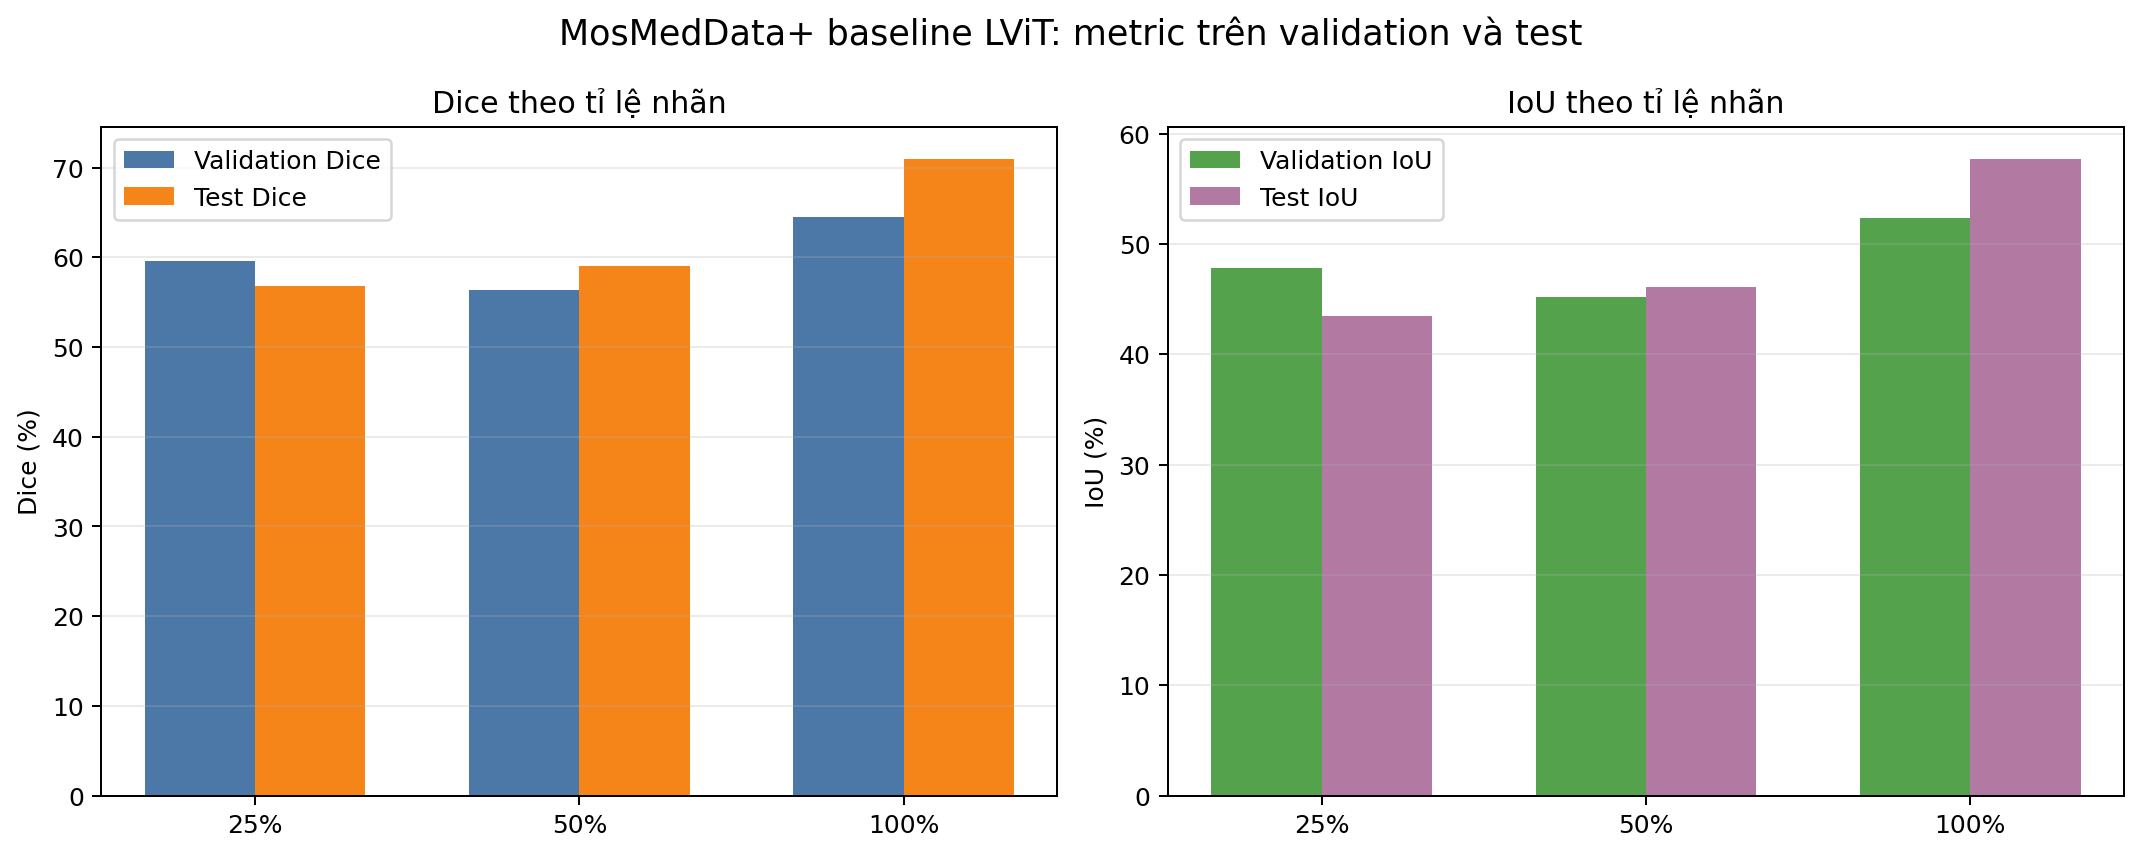
\includegraphics[width=0.94\textwidth]{figures/mosmed_baseline_scores.png}
  \caption{Dice và IoU của baseline LViT trên MosMedData+ theo ba mức nhãn. Điểm test tăng rõ nhất ở mốc 100\%, trong khi 25\% và 50\% còn khá sát nhau.}
  \label{fig:mosmed-baseline-scores}
\end{figure}

\begin{figure}[H]
  \centering
  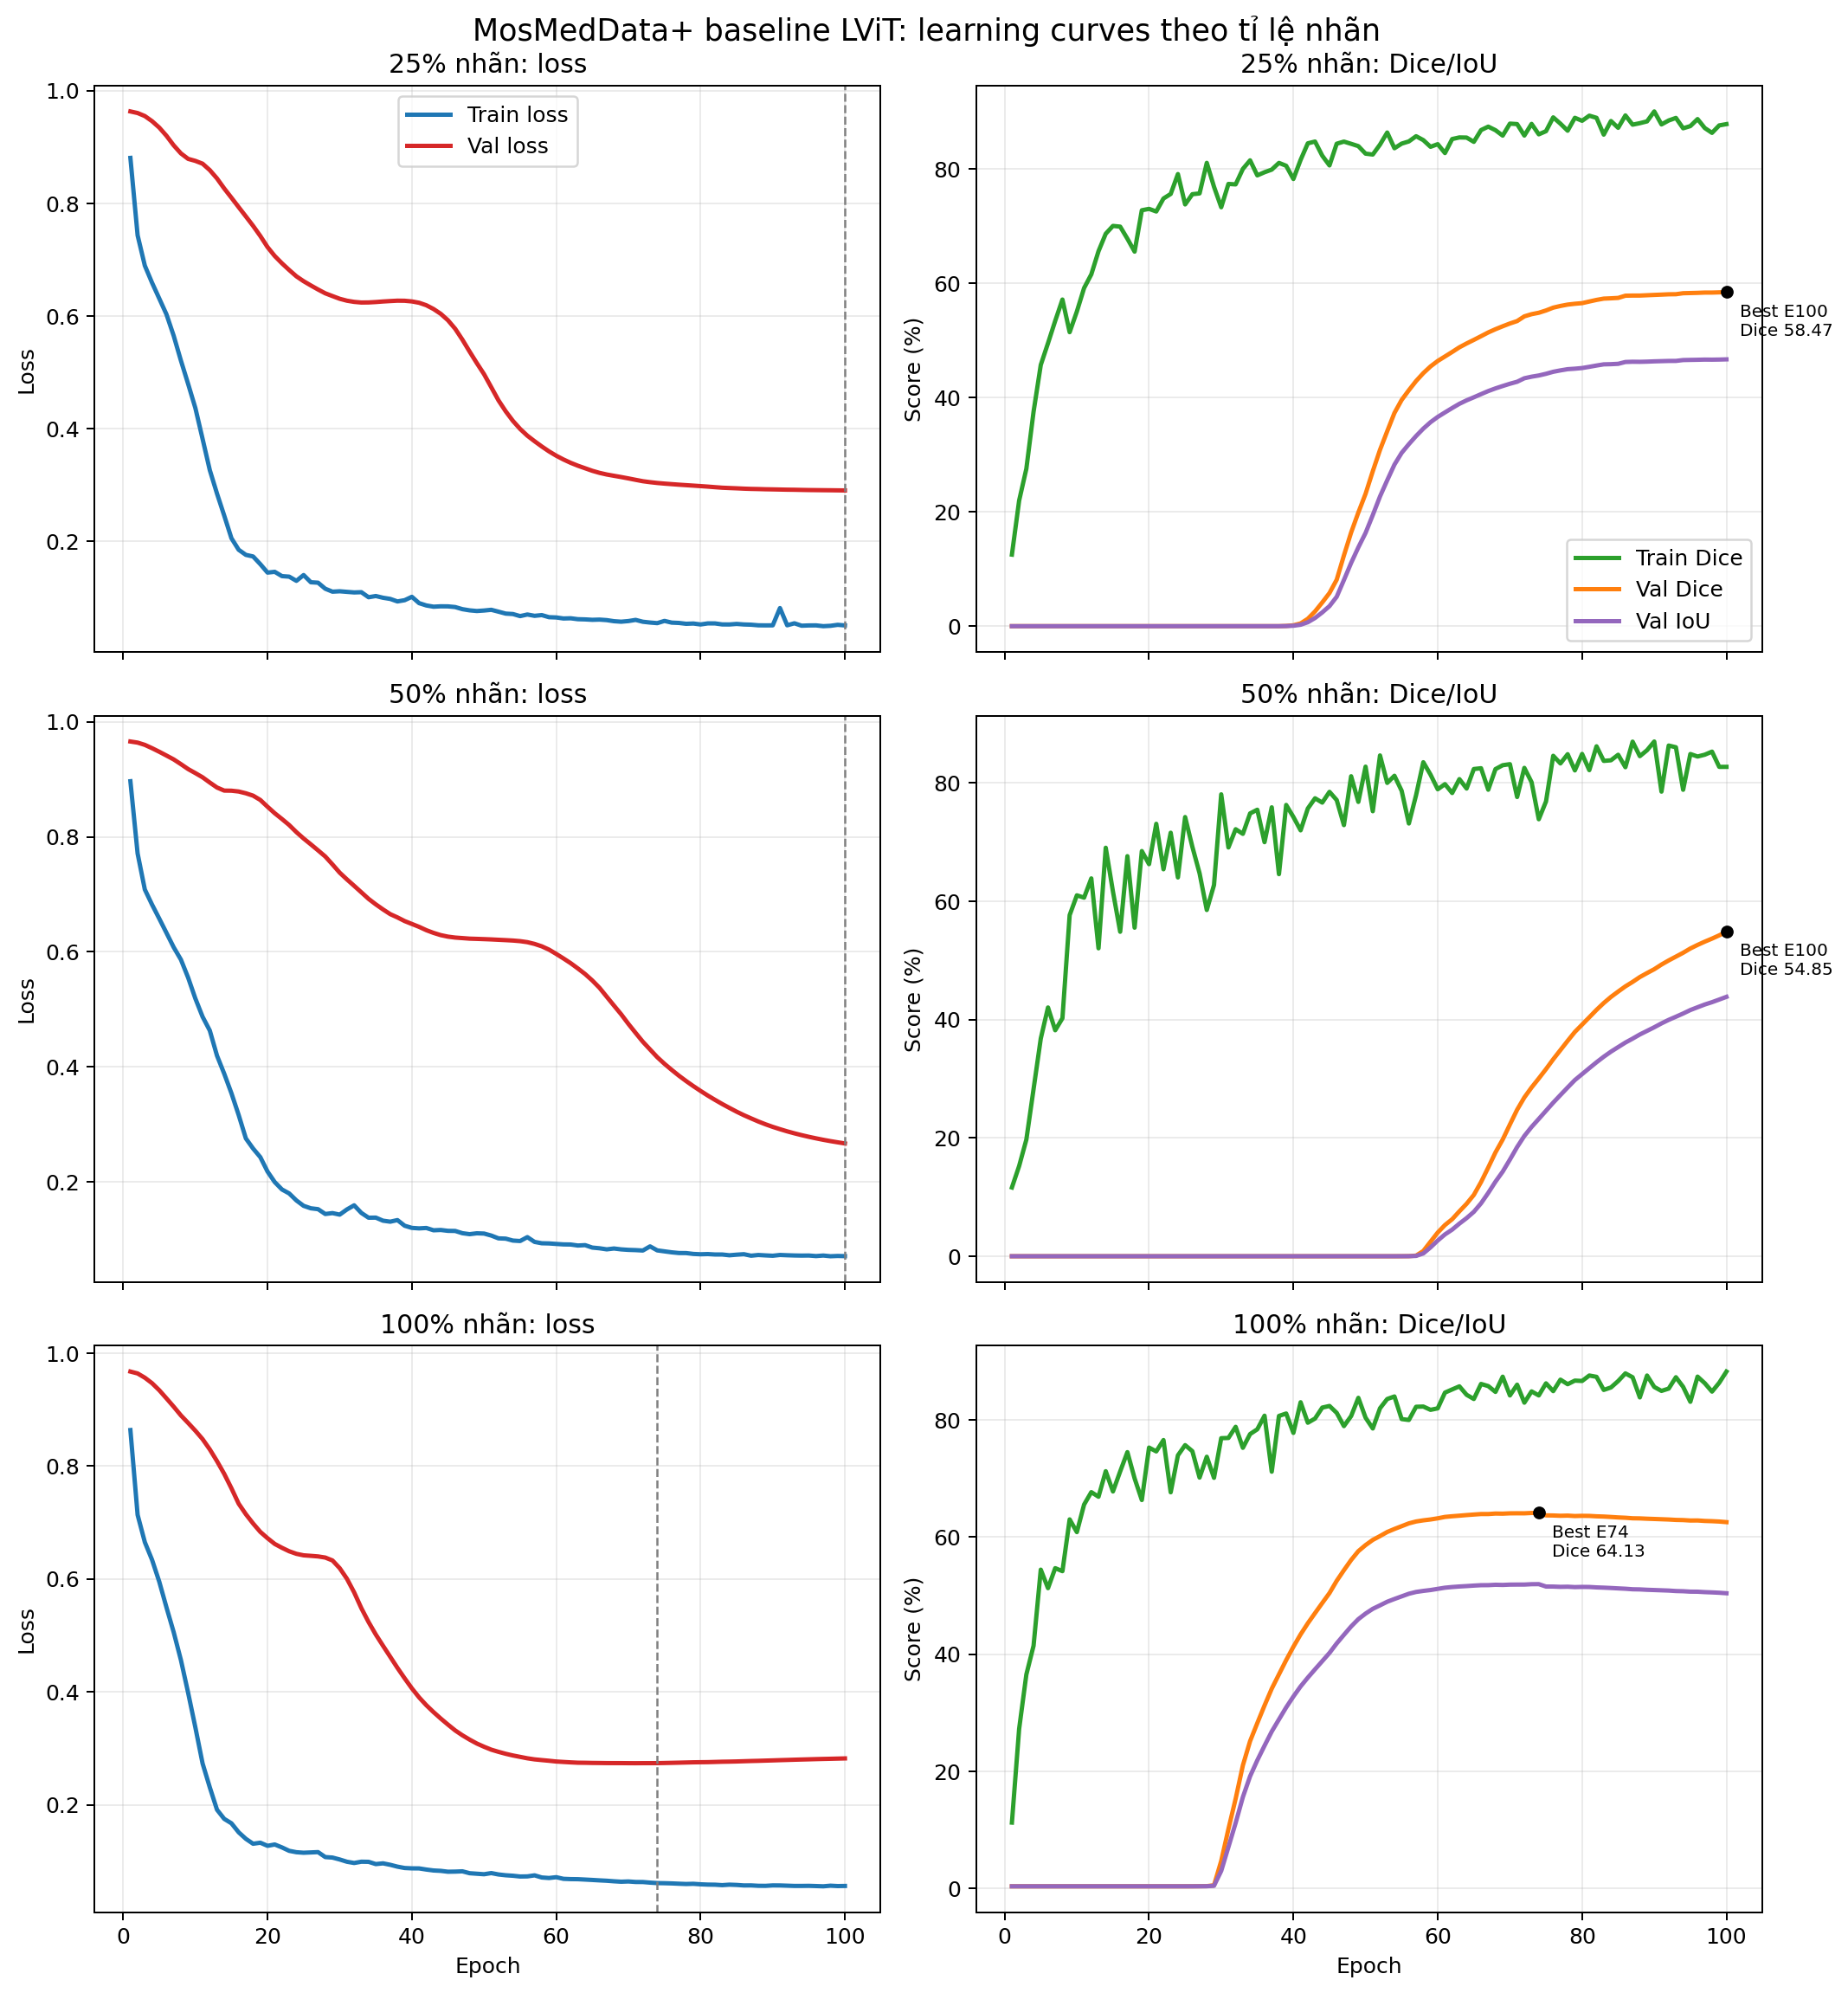
\includegraphics[width=0.96\textwidth]{figures/mosmed_baseline_training_curves.png}
  \caption{Learning curves của baseline LViT trên MosMedData+ ở ba mức nhãn. Mỗi hàng tương ứng một tỉ lệ nhãn; cột trái là loss, cột phải là Dice/IoU.}
  \label{fig:mosmed-baseline-training-curves}
\end{figure}

Hình~\ref{fig:mosmed-baseline-training-curves} giúp đọc sâu hơn bảng số cuối. Ở 25\% và 50\% nhãn, validation Dice tốt nhất đều xuất hiện ở epoch cuối, lần lượt khoảng 58.47 và 54.85. Điều này cho thấy baseline chưa thật sự hội tụ mạnh vào một vùng ổn định cao như trên QaTa-COV19; mô hình tiến bộ dần nhưng trần validation còn thấp. Ở 100\% nhãn, validation Dice đạt đỉnh khoảng 64.13 tại epoch 74 rồi giảm nhẹ về 62.55 ở epoch cuối. Mẫu hình này nói rằng trên CT, thêm nhãn thật giúp nâng trần chất lượng, nhưng huấn luyện vẫn nhạy với việc giữ biên và kiểm soát vùng foreground nhỏ.

\begin{figure}[H]
  \centering
  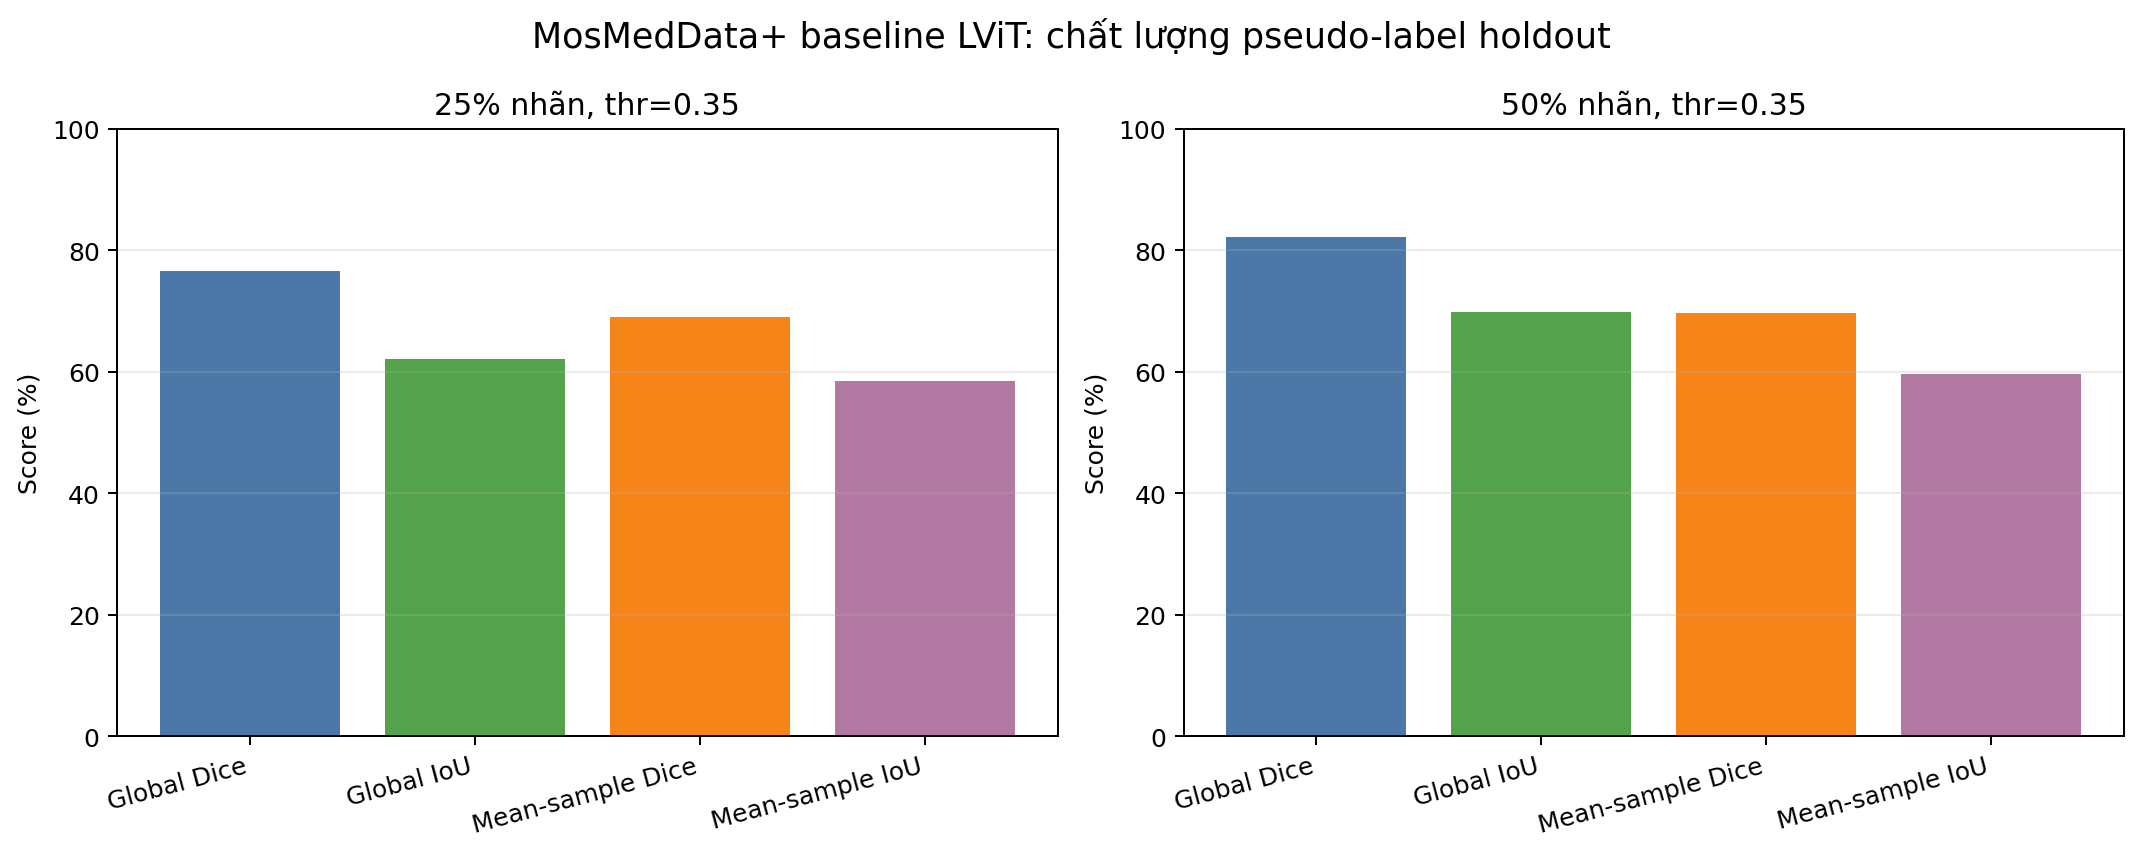
\includegraphics[width=0.82\textwidth]{figures/mosmed_baseline_pseudo_holdout.png}
  \caption{Chất lượng pseudo-label holdout của baseline LViT trên MosMedData+ ở 25\% và 50\% nhãn. Với 100\% nhãn không còn mẫu chưa nhãn nên không có pseudo-label holdout.}
  \label{fig:mosmed-baseline-pseudo}
\end{figure}

\begin{figure}[H]
  \centering
  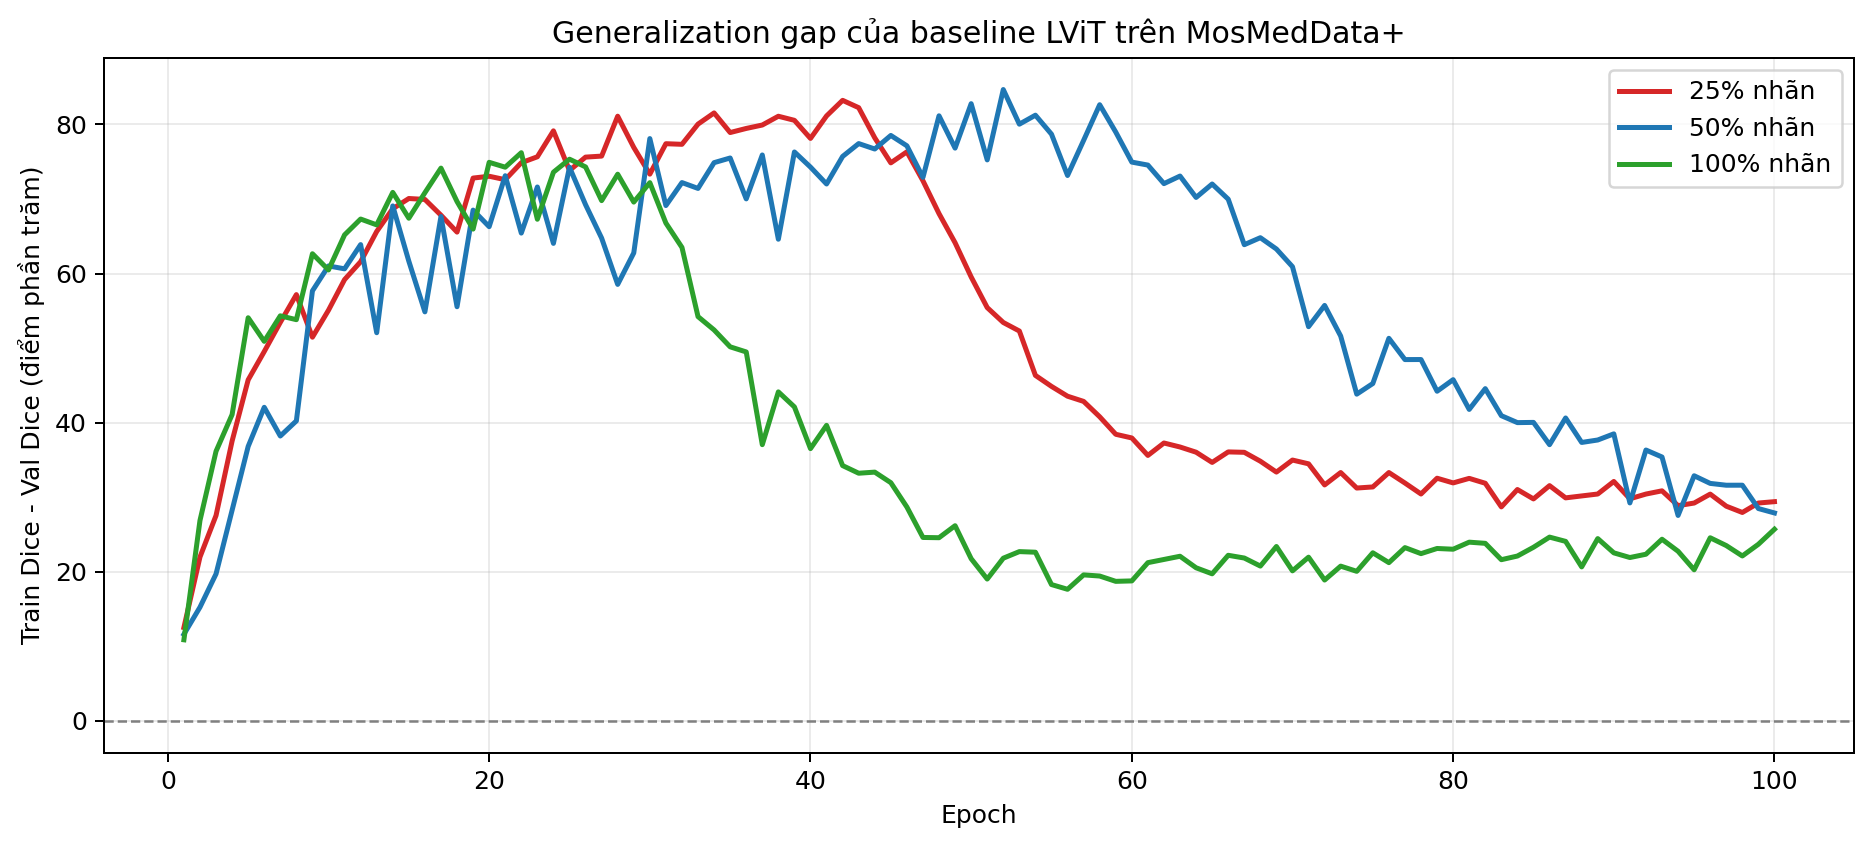
\includegraphics[width=0.80\textwidth]{figures/mosmed_baseline_generalization_gap.png}
  \caption{Generalization gap của baseline LViT trên MosMedData+: chênh lệch giữa train Dice và validation Dice theo epoch. Khoảng cách lớn kéo dài cho thấy CT khó hơn và dễ overfit hơn X-quang.}
  \label{fig:mosmed-baseline-gap}
\end{figure}

Pseudo-label holdout trong Hình~\ref{fig:mosmed-baseline-pseudo} cho thêm một insight quan trọng. Ở 25\% nhãn, global Dice của pseudo-label đạt khoảng 76.65 nhưng mean-sample Dice chỉ khoảng 69.10; ở 50\% nhãn, global Dice tăng lên khoảng 82.24 nhưng mean-sample Dice vẫn chỉ quanh 69.72. Điều này cho thấy trên CT, pseudo-label có thể đúng khá nhiều ở tổng điểm ảnh nhưng vẫn không đồng đều giữa các lát. Nói cách khác, một số lát được dự đoán tốt, còn một số lát foreground nhỏ hoặc phân mảnh kéo mạnh sample-level metric xuống. Hình~\ref{fig:mosmed-baseline-gap} củng cố nhận xét này: khoảng cách train--validation lớn hơn hẳn QaTa-COV19, nhất là trong giai đoạn giữa của quá trình học, cho thấy baseline trên CT dễ học mạnh vào các pattern cục bộ của tập train nhưng khó tổng quát đều sang validation.

\textbf{Kết quả chính của recipe cải tiến trên MosMedData+.} Sau khi đã có baseline chạy lại để hiểu hành vi của LViT trên CT, phần cải tiến được đọc như một chuỗi thay đổi nhằm giải quyết đúng các lỗi vừa quan sát: nền ngoài phổi còn gây nhiễu, pseudo-label chưa đều giữa các lát, generalization gap còn lớn và metric còn nhạy với ngưỡng nhị phân hóa. Vì vậy, bảng kết quả dưới không chỉ là danh sách recipe, mà là lộ trình từ baseline CT sang một pipeline ổn định hơn.

\begin{table}[H]
  \centering
  \caption{Các thiết lập cải tiến trên MosMedData+ theo tỉ lệ nhãn. Giá trị là test Dice/IoU, đơn vị phần trăm.}
  \label{tab:mosmed-ablation}
  \scriptsize
  \renewcommand{\arraystretch}{1.12}
  \setlength{\tabcolsep}{4pt}
  \begin{tabularx}{\textwidth}{@{}L Y L Y@{}}
    \toprule
    Thiết lập & Nhãn & Ghi chú đánh giá & Dice/IoU \\
    \midrule
    BiomedBERT variant ban đầu & 50\% & Dùng BiomedBERT để mã hóa văn bản nhưng pipeline ảnh/nhãn giả còn gần bản đầu, chưa thêm crop và cleanup đầy đủ & 68.88 / 55.14 \\
    BiomedBERT + crop-only + pseudo threshold & 50\% & Thêm crop vùng phổi để giảm nền CT ngoài phổi; hiệu chỉnh cách tạo nhãn giả để bớt lan false positive & 70.36 / 56.97 \\
    BiomedBERT student-only + loss cleanup + crop-only & 50\% & Bỏ teacher/EMA không ổn định trên CT, chỉ huấn luyện student; làm sạch loss và giữ crop vùng phổi & 72.85 / 59.41 \\
    NoBERT student-only + fixed threshold & 50\% & Thay BiomedBERT bằng bộ mã hóa nhẹ học từ dữ liệu đích; giữ student-only để kiểm tra vai trò bộ mã hóa văn bản & 72.99 / 59.48 \\
    BiomedBERT student-only + loss cleanup + crop-only + LightAU & 25\% & Recipe cải tiến cuối trên CT: BiomedBERT, student-only, loss cleanup, crop vùng phổi và augmentation nhẹ & 65.50 / 51.32 \\
    BiomedBERT student-only + loss cleanup + crop-only + LightAU & 50\% & Recipe cải tiến cuối trên CT với 50\% mask thật; đây là cấu hình MosMedData+ tốt nhất trong báo cáo & \textbf{73.84 / 60.31} \\
    BiomedBERT student-only + loss cleanup + crop-only + LightAU & 100\% & Cùng recipe cải tiến cuối nhưng dùng toàn bộ mask train để kiểm tra nút thắt còn lại của miền CT & 73.60 / 60.12 \\
    NoBERT student-only + LightAU & 50\% & Giữ augmentation nhẹ nhưng dùng bộ mã hóa văn bản nhẹ, nhằm so sánh với BiomedBERT khi văn bản chú thích có cấu trúc mạnh & 72.77 / 59.22 \\
    \bottomrule
  \end{tabularx}
\end{table}
\FloatBarrier

Trên MosMedData+, cải tiến diễn ra theo từng lớp nên tên cấu hình cần được đọc theo đúng thành phần. \textit{Crop-only} không phải là một mô hình mới; nó là bước tiền xử lý cắt/giữ vùng phổi để giảm nền CT ngoài cơ thể và làm foreground tổn thương chiếm tỉ lệ có ý nghĩa hơn. \textit{Student-only} nghĩa là trong thử nghiệm CT này, mô hình học trực tiếp bằng student thay vì phụ thuộc mạnh vào teacher/EMA; lựa chọn này xuất phát từ quan sát pseudo-label trên CT dễ kém ổn định hơn X-quang. \textit{Loss cleanup} là nhóm thay đổi làm loss gọn và ổn định hơn, tránh để các thành phần phụ trợ yếu hoặc nhiễu chi phối loss chính. \textit{LightAU} là augmentation nhẹ theo tinh thần nnU-Net: tăng đa dạng cường độ/hình học vừa phải, nhưng không biến dạng lát CT quá mạnh.

Với cách đọc đó, kết quả trong Bảng~\ref{tab:mosmed-ablation} cho thấy BiomedBERT ban đầu đạt 68.88 Dice; thêm crop và hiệu chỉnh pseudo-label tăng lên 70.36; chuyển sang student-only với loss cleanup tăng tiếp lên 72.85; và recipe cuối với LightAU đạt tốt nhất ở 50\% nhãn: 73.84 Dice và 60.31 IoU. So với baseline chạy lại cùng mức 50\%, recipe cuối tăng khoảng \(+14.82\) điểm Dice và \(+14.20\) điểm IoU. Khoảng cách lớn này nói rõ rằng trên CT, bản thân việc ``có văn bản'' chưa đủ; pipeline còn phải ổn định ở tiền xử lý ảnh, nhãn giả và hậu xử lý xác suất.

Ở mức 25\% nhãn, recipe cuối đạt 65.50/51.32, cao hơn baseline 25\% là 56.76/43.48. Ở mức 100\% nhãn, kết quả 73.60/60.12 cũng cao hơn baseline 100\% là 70.98/57.71 nhưng chênh lệch nhỏ hơn. Điều này khá giống tinh thần chung của LViT: cải tiến tạo lợi lớn nhất khi nhãn hạn chế, còn khi đã có đủ mask hơn thì nút thắt dịch dần sang đặc tính riêng của miền CT như mask phân mảnh, foreground nhỏ và sai số biên.

Riêng về bộ mã hóa văn bản trên MosMedData+, NoBERT với ngưỡng cố định đạt 72.99/59.48, hơi cao hơn dòng BiomedBERT student-only 72.85/59.41 trước khi thêm LightAU. Điều này khác với QaTa-COV19, nơi BiomedBERT nhỉnh hơn NoBERT. Kết quả này cho thấy bộ mã hóa văn bản mạnh không tự động thắng nếu domain ảnh, prompt format, threshold và preprocessing chưa khớp. Với MosMedData+, yếu tố ổn định ảnh CT và ngưỡng dự đoán có thể quan trọng ngang hoặc hơn lựa chọn bộ mã hóa văn bản.

\begin{figure}[H]
  \centering
  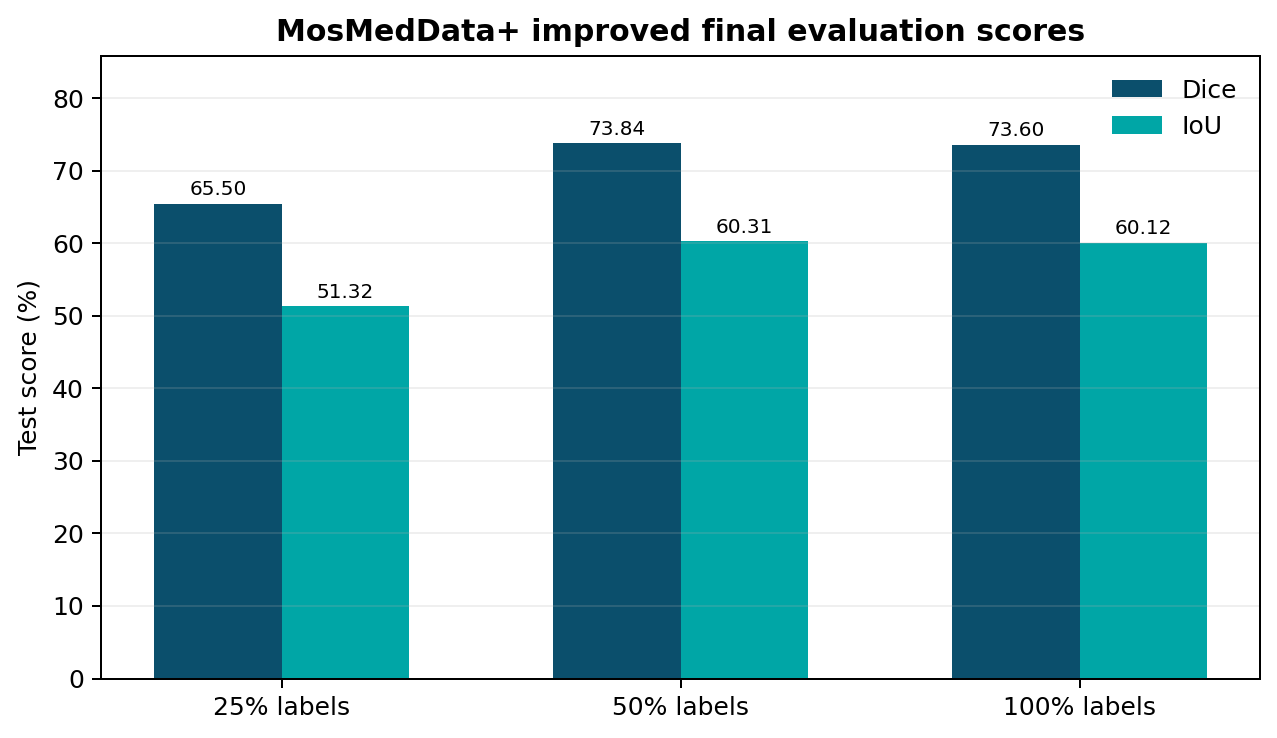
\includegraphics[width=0.78\textwidth]{figures/mosmed_improved_scores.png}
  \caption{Kết quả Dice/IoU của recipe cải tiến trên MosMedData+ ở các mức 25\%, 50\% và 100\% nhãn.}
  \label{fig:mosmed-improved-scores}
\end{figure}

\begin{figure}[H]
  \centering
  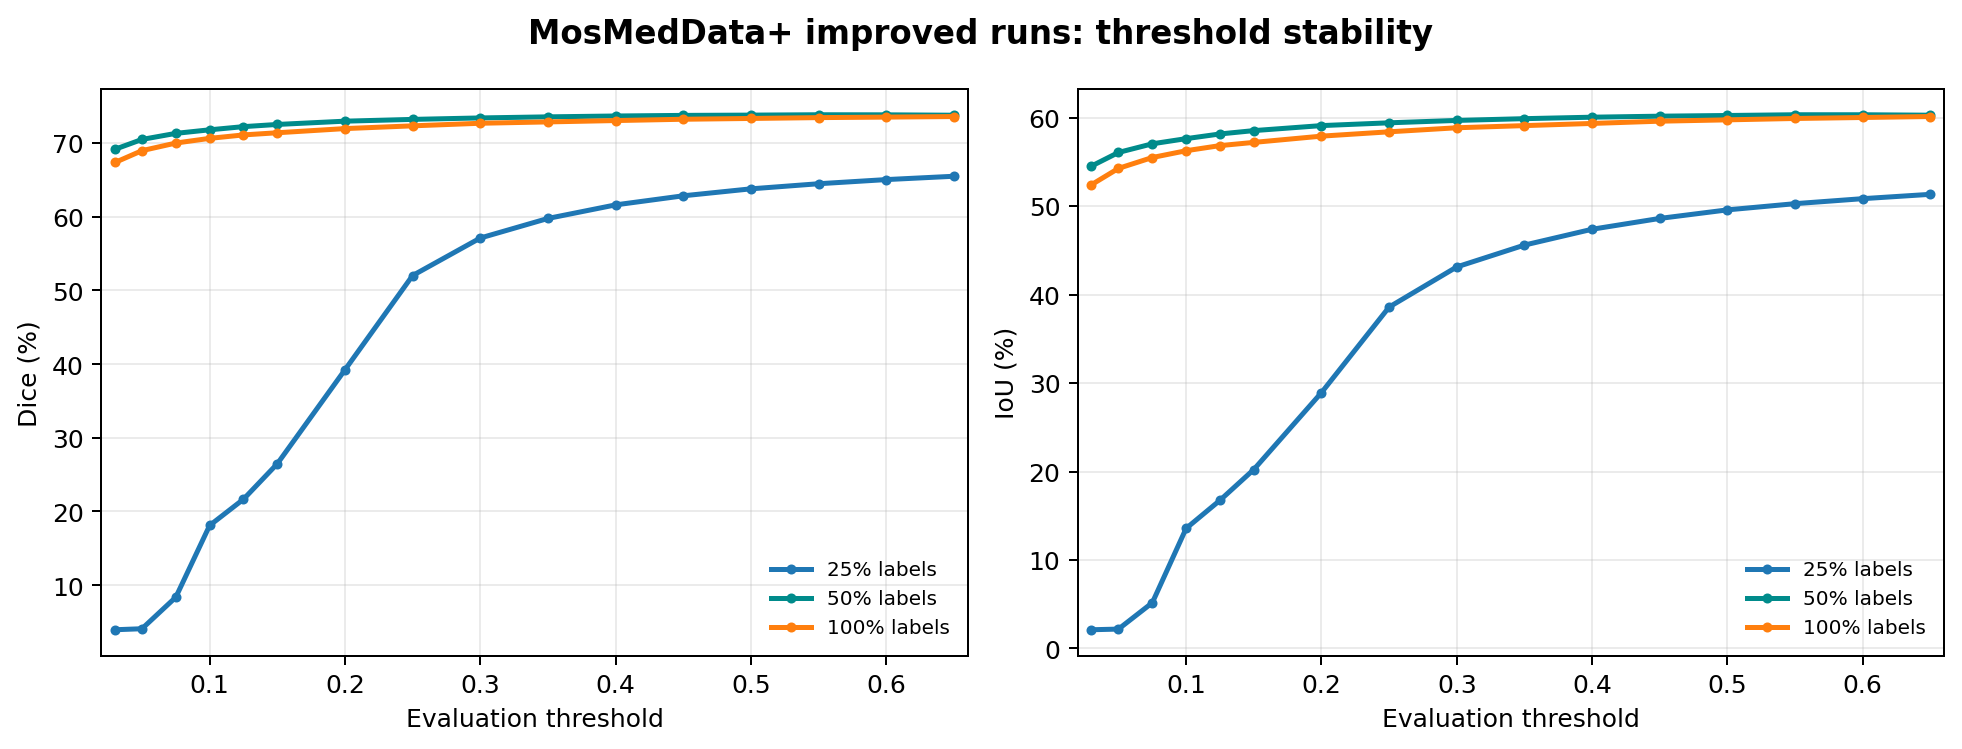
\includegraphics[width=0.94\textwidth]{figures/mosmed_improved_threshold_curves.png}
  \caption{Độ nhạy của Dice/IoU theo ngưỡng nhị phân hóa trên MosMedData+. Đường cong cho thấy CT nhạy với ngưỡng, đặc biệt khi số nhãn ít.}
  \label{fig:mosmed-improved-threshold}
\end{figure}

\begin{figure}[H]
  \centering
  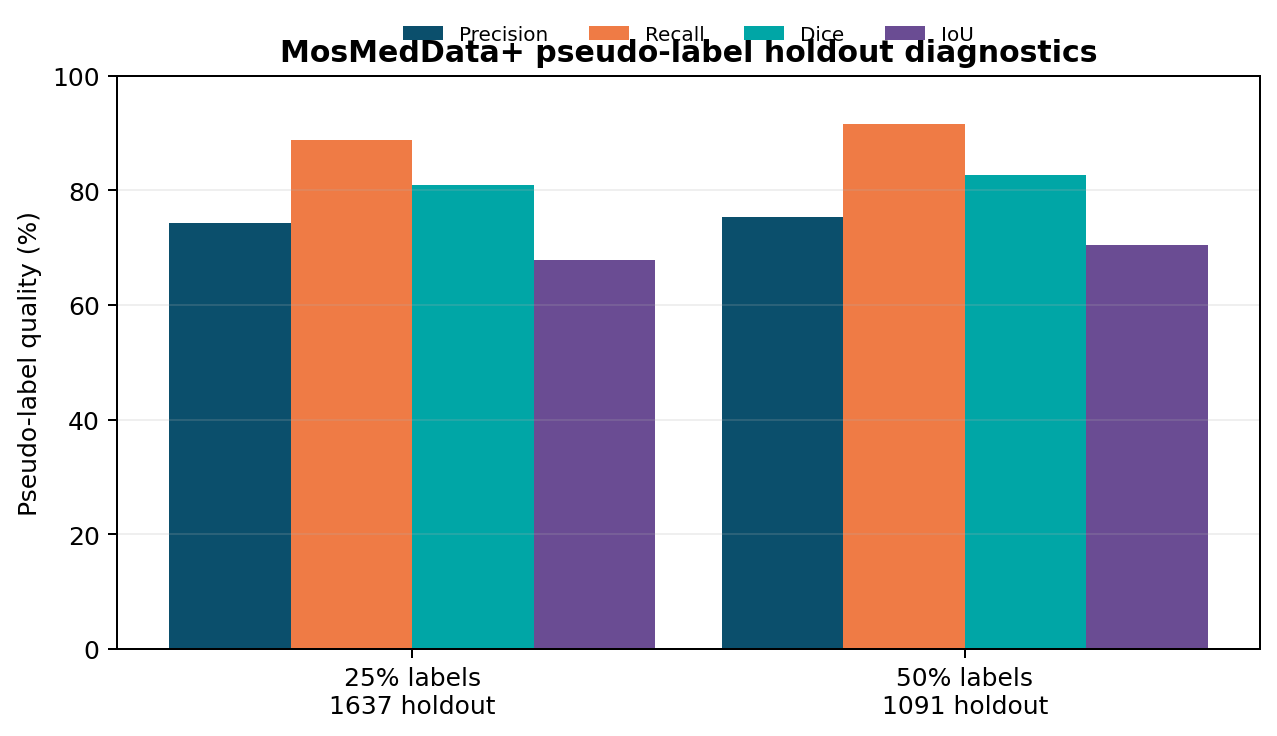
\includegraphics[width=0.82\textwidth]{figures/mosmed_improved_pseudo_holdout.png}
  \caption{Chẩn đoán pseudo-label trên phần holdout của MosMedData+ ở các mức có dữ liệu chưa nhãn.}
  \label{fig:mosmed-improved-pseudo}
\end{figure}

\begin{figure}[H]
  \centering
  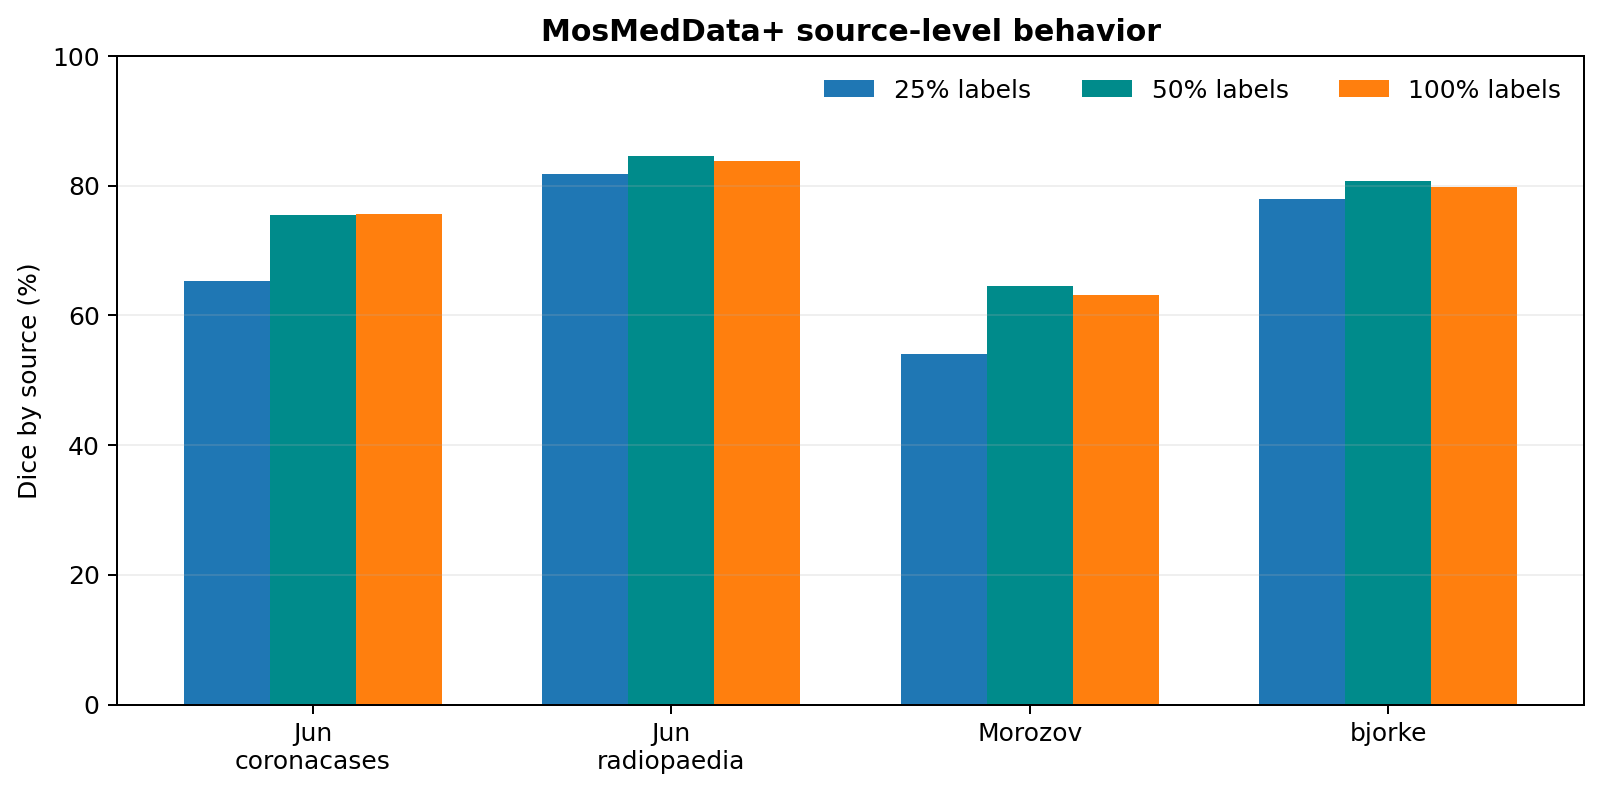
\includegraphics[width=0.88\textwidth]{figures/mosmed_improved_source_behavior.png}
  \caption{Hành vi theo nguồn con của MosMedData+. Các nguồn CT khác nhau tạo độ khó khác nhau, nên cần đọc kết quả MosMedData+ như một bài kiểm tra đa nguồn thay vì một tập đồng nhất.}
  \label{fig:mosmed-improved-source}
\end{figure}

\begin{figure}[H]
  \centering
  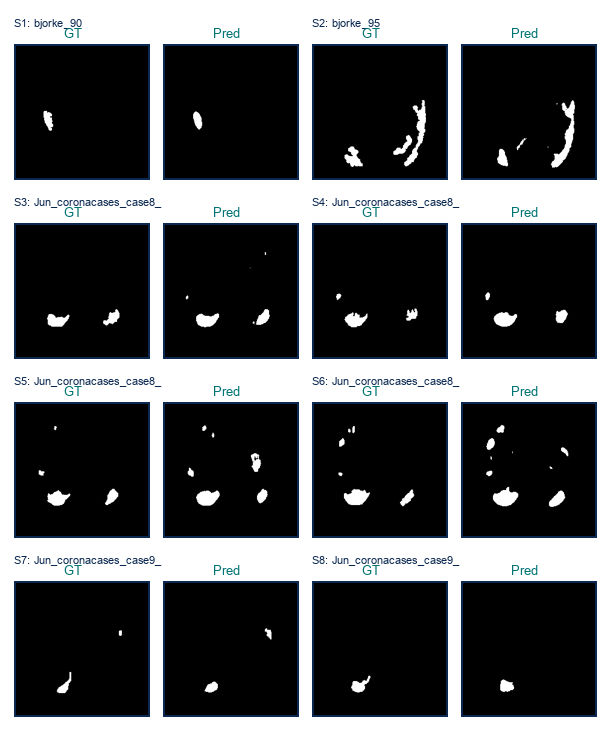
\includegraphics[width=0.74\textwidth]{figures/mosmed_improved_val_artifacts.png}
  \caption{Một số artifact định tính của MosMedData+ 50\%: mask thật và mask dự đoán. Các ví dụ cho thấy dự đoán tốt hơn ở vùng tổn thương rõ, nhưng vẫn dễ nhạy với cụm nhỏ hoặc biên mờ.}
  \label{fig:mosmed-improved-artifacts}
\end{figure}

\FloatBarrier

\begin{table}[H]
  \centering
  \caption{So sánh baseline chạy lại và recipe cải tiến trên MosMedData+ theo nhiều khía cạnh.}
  \label{tab:mosmed-baseline-vs-improved}
  \small
  \renewcommand{\arraystretch}{1.15}
  \setlength{\tabcolsep}{4pt}
  \begin{tabularx}{\textwidth}{@{}L Y Y@{}}
    \toprule
    Khía cạnh so sánh & Baseline LViT chạy lại & Recipe cải tiến trên MosMedData+ \\
    \midrule
    Metric test & 25\%: 56.76 / 43.48; 50\%: 59.01 / 46.11; 100\%: 70.98 / 57.71 & 25\%: 65.50 / 51.32; 50\%: 73.84 / 60.31; 100\%: 73.60 / 60.12 \\
    Hành vi học & Generalization gap lớn; 25\% và 50\% còn hội tụ chậm; 100\% đạt đỉnh ở epoch 74 rồi giảm nhẹ & Pipeline ổn định hơn nhờ crop, cleanup, LightAU và student-only; 50\% trở thành mốc tốt nhất \\
    Pseudo-label & Global Dice tăng từ 76.65 lên 82.24 khi tăng nhãn từ 25\% lên 50\%, nhưng mean-sample Dice vẫn quanh 69--70 & Pseudo-label được kiểm soát thêm bằng threshold, cleanup và recipe phù hợp miền CT nên hữu ích hơn cho Dice/IoU cuối \\
    Độ nhạy miền CT & Rất nhạy với foreground nhỏ và khác biệt giữa các lát; điểm 50\% chưa vượt rõ 25\% trên validation & Có thêm source-level behavior và threshold analysis để đọc rõ CT đa nguồn khó ở đâu \\
    Ý nghĩa & Cho thấy baseline ảnh--văn bản trên CT đã có tín hiệu, nhưng còn xa mức đủ ổn định để cạnh tranh mạnh & Chứng minh rằng phải đồng thời xử lý ảnh, pseudo-label và ngưỡng thì lợi ích của hướng ảnh--văn bản mới bộc lộ trên CT \\
    \bottomrule
  \end{tabularx}
\end{table}
\FloatBarrier

\subsection{Nhận xét và phân tích}

Về độ chính xác, các ablation cho thấy cải tiến mạnh nhất ở điều kiện ít nhãn. Đây là kết quả phù hợp với động lực của LViT: khi mask ít, văn bản và pseudo-label có giá trị hơn. Tuy nhiên, kết quả cũng cho thấy văn bản không phải luôn có lợi tuyệt đối. B0 thấp hơn baseline là ví dụ rõ: nếu prompt/văn bản chưa chuẩn hóa, mô hình có thể nhận tín hiệu nhiễu và học kém hơn. Vì vậy, kết luận đúng không phải ``thêm văn bản là tốt'', mà là ``văn bản cần được chuẩn hóa, mã hóa và đưa vào đúng cách''.

Về độ phức tạp, QaTaLViT cải tiến tốn hơn baseline thuần vì thêm hoặc làm nặng một số khối: BiomedBERT/cache embedding, cross-modal fusion, prior không gian, pseudo-label fusion và augmentation. Đổi lại, phần tăng chi phí đem lại cải thiện Dice/IoU có thể đo được. Với đồ án môn học, điều quan trọng là chỉ ra trade-off: mô hình không miễn phí về tính toán, nhưng có cơ sở khi bài toán thiếu nhãn và giàu ngữ cảnh lâm sàng.

Về giới hạn, các kết quả thực nghiệm vẫn cần được đọc thận trọng. Một số số liệu được tổng hợp từ các lần chạy đã khóa, nhưng điều kiện phần cứng, môi trường thư viện và split dữ liệu có thể khác paper gốc. Trên MosMedData+, metric còn nhạy với ngưỡng nhị phân hóa và nguồn con của dữ liệu CT, nên kết quả cần được hiểu cùng với đường cong threshold và phân tích source-level. Ngoài ra, các biến thể I2--I5 chưa phải một ablation cô lập hoàn hảo từng thay đổi nhỏ; chúng là các cấu hình thực nghiệm theo nhóm thay đổi. Vì vậy, bảng ablation nên được hiểu là bằng chứng định hướng, không phải chứng minh nhân quả tuyệt đối cho từng module nhỏ.

\section{Kết luận chương}

Chương 4 trả lời câu hỏi thực nghiệm trung tâm của báo cáo: LViT có thể được tái hiện như một pipeline ảnh--văn bản đầy đủ hay không, và phần cải tiến đề xuất có thật sự làm tốt hơn ở những điểm yếu đã phân tích hay không. Kết quả cho thấy câu trả lời là có, nhưng không theo nghĩa một module đơn lẻ luôn thắng trong mọi hoàn cảnh. Trên QaTa-COV19, nơi văn bản chú thích khớp khá tốt với mask và bài toán thiếu nhãn thể hiện rõ, QaTaLViT cải thiện ổn định ở cả 25\%, 50\% và 100\% nhãn. Trên MosMedData+, nơi dữ liệu là CT đa nguồn, mask nhỏ và phân mảnh hơn, cải tiến vẫn cho kết quả cạnh tranh nhưng nhạy hơn với crop, augmentation và ngưỡng nhị phân hóa.

\begin{table}[H]
  \centering
  \caption{Tổng hợp kết quả chính rút ra từ Chương 4. Giá trị là test Dice/IoU, đơn vị phần trăm.}
  \label{tab:chapter4-conclusion-summary}
  \scriptsize
  \renewcommand{\arraystretch}{1.12}
  \setlength{\tabcolsep}{4pt}
  \begin{tabularx}{\textwidth}{@{}p{0.18\textwidth} p{0.16\textwidth} Y Y Y@{}}
    \toprule
    Tập dữ liệu & Thiết lập & Mốc so sánh & Kết quả cải tiến & Chênh lệch chính \\
    \midrule
    QaTa-COV19 & 25\% nhãn & LViT: 78.42 / 68.43 & QaTaLViT: 82.22 / 73.35 & \(+3.80\) Dice, \(+4.92\) IoU; tương đối khoảng \(+4.85\%\) Dice và \(+7.19\%\) IoU \\
    QaTa-COV19 & 50\% nhãn & LViT: 80.32 / 70.60 & QaTaLViT: 84.03 / 75.62 & \(+3.71\) Dice, \(+5.02\) IoU; tương đối khoảng \(+4.62\%\) Dice và \(+7.11\%\) IoU \\
    QaTa-COV19 & 100\% nhãn & LViT: 82.76 / 73.78 & QaTaLViT: 85.28 / 77.25 & \(+2.52\) Dice, \(+3.47\) IoU; tương đối khoảng \(+3.05\%\) Dice và \(+4.70\%\) IoU \\
    MosMedData+ & 50\% nhãn & U-Net: 64.60 / 50.73; LViT-T 50\%: 73.56 / 61.05 & Recipe cải tiến: 73.84 / 60.31 & Hơn U-Net \(+9.24\) Dice, \(+9.58\) IoU; so với LViT-T 50\%, Dice \(+0.28\) nhưng IoU \(-0.74\) \\
    \bottomrule
  \end{tabularx}
\end{table}
\FloatBarrier

Insight quan trọng nhất từ bảng tổng hợp là mức tăng của QaTaLViT lớn nhất khi dữ liệu có nhãn ít. Ở 25\% và 50\% nhãn, IoU tăng hơn 4.9--5.0 điểm phần trăm, tức là cải tiến không chỉ làm dự đoán ``trông mượt hơn'' mà thật sự tăng vùng chồng lấn đúng giữa mask dự đoán và mask chuyên gia. Khi lên 100\% nhãn, mức tăng giảm còn \(+2.52\) Dice và \(+3.47\) IoU, nhưng vẫn dương. Điều này cho thấy các module cải tiến không chỉ là cơ chế bù thiếu nhãn; chúng còn giúp biểu diễn ảnh--văn bản tốt hơn ngay cả khi có đủ mask hơn. Tuy nhiên, độ lợi giảm ở 100\% cũng nói rõ giới hạn: khi giám sát mức điểm ảnh đã mạnh, vai trò của văn bản và pseudo-label không còn áp đảo như ở thiết lập ít nhãn.

Ưu điểm rõ nhất của phương pháp cải tiến nằm ở bốn điểm. Thứ nhất, chuẩn hóa prompt giúp biến văn bản chú thích từ chuỗi mô tả dễ nhiễu thành tín hiệu ngữ nghĩa ổn định hơn; kết quả B0 thấp hơn baseline nhưng I1 tăng lại cho thấy bước này không phải chi tiết phụ. Thứ hai, BiomedBERT và các cơ chế fusion giúp văn bản đi vào biểu diễn ảnh trước bộ giải mã, nên mô hình có cơ hội điều chỉnh vùng dự đoán thay vì chỉ dùng văn bản như thông tin phụ ở cuối mạng. Thứ ba, prior/skip adapter và kiểm soát pseudo-label đánh đúng các lỗi quan sát được ở baseline: dự đoán lan rộng, bỏ sót cụm nhỏ và biên chưa sắc. Thứ tư, phân tích artifact cho thấy cải tiến có ý nghĩa ở nhiều mặt: điểm số cuối, hành vi học, chất lượng pseudo-label và hình dạng mask dự đoán.

Điểm hạn chế cũng cần nhìn thẳng. Phương pháp cải tiến làm pipeline nặng hơn LViT gốc vì thêm bộ mã hóa văn bản, fusion, prior, adapter, kiểm soát pseudo-label và augmentation; do đó lợi ích về Dice/IoU phải được đánh đổi bằng chi phí tính toán và độ phức tạp triển khai. Các ablation I2--I5 là ablation theo nhóm thay đổi, nên chúng chỉ cho bằng chứng định hướng về nhóm module hữu ích, chưa chứng minh nhân quả tuyệt đối cho từng lớp nhỏ. Trên MosMedData+, recipe cải tiến vượt xa U-Net và nhỉnh hơn nhẹ LViT-T 50\% về Dice, nhưng IoU vẫn thấp hơn. Điều này cho thấy mô hình có thể bắt được vùng tổn thương chính, nhưng mức chồng lấn nghiêm ngặt vẫn bị ảnh hưởng bởi biên mask, vùng dự đoán lan rộng hoặc bỏ sót cụm nhỏ. Khi chuyển từ X-quang sang CT, nút thắt không còn chỉ là bộ mã hóa văn bản hay pseudo-label, mà còn là phân bố ảnh đa nguồn, foreground rất nhỏ, mask phân mảnh và độ nhạy với ngưỡng nhị phân hóa. Vì vậy, kết luận đúng của Chương 4 là: cải tiến đề xuất có hiệu quả rõ trên QaTa-COV19 và đem lại phân tích có giá trị trên MosMedData+, nhưng để trở thành một phương pháp tổng quát mạnh trên CT cần thêm hiệu chuẩn xác suất, kiểm soát miền dữ liệu và ablation cô lập hơn.

\chapter{Kết luận và hướng phát triển}
\label{sec:conclusion}

Chương cuối tổng hợp lại toàn bộ mạch lập luận của báo cáo: vì sao LViT là một hướng đáng chú ý trong phân đoạn ảnh y khoa, phương pháp này giải quyết bài toán theo triết lý nào, các thử nghiệm cho thấy điều gì, và những giới hạn nào cần được xử lý nếu muốn phát triển tiếp. Điểm quan trọng nhất cần giữ lại là LViT không chỉ là một biến thể kiến trúc của U-Net hay Transformer. LViT đại diện cho một cách nhìn rộng hơn: trong y khoa, ảnh, văn bản lâm sàng và mặt nạ chuyên gia là ba nguồn thông tin có vai trò khác nhau; mô hình tốt cần biết phối hợp chúng thay vì chỉ học từ ảnh một cách cô lập.

\section{Kết luận}

Bài toán được khảo sát trong báo cáo là phân đoạn ảnh y khoa có văn bản đi kèm. Đầu vào của hệ thống gồm ảnh y khoa \(x\) và văn bản chú thích \(t\); trong giai đoạn học có thể có thêm mặt nạ chuyên gia \(y\). Đầu ra cần dự đoán là mặt nạ phân đoạn \(\hat{y}\), biểu diễn vùng tổn thương ở mức điểm ảnh. Đây là bài toán khó vì vùng bệnh thường nhỏ, biên mờ, foreground mất cân bằng mạnh so với nền, và nhãn phân đoạn mức điểm ảnh rất tốn công thu thập. Trong bối cảnh đó, văn bản y khoa trở thành một nguồn tín hiệu đáng giá: nó không thay thế được mask, nhưng có thể cung cấp ngữ cảnh về vị trí, mức độ lan rộng và đặc điểm tổn thương.

LViT giải quyết bài toán bằng cách kết hợp ba ý tưởng chính. Thứ nhất, mô hình giữ lại sức mạnh cục bộ của CNN/Double-U để bảo toàn chi tiết không gian và phục hồi mask ở bộ giải mã. Thứ hai, mô hình dùng Transformer để học quan hệ xa giữa các vùng ảnh, giúp xử lý các cấu trúc tổn thương phân bố không liền mạch. Thứ ba, mô hình đưa văn bản vào quá trình học qua LV Fusion và dùng văn bản trong học bán giám sát thông qua EPI/LV loss để kiểm soát pseudo-label. Nhờ vậy, LViT không xem văn bản chú thích là phần mô tả phụ, mà biến nó thành tín hiệu ảnh hưởng trực tiếp đến biểu diễn và quá trình tối ưu.

Báo cáo đã triển khai nội dung theo đúng logic của một hệ thống hoàn chỉnh. Chương 1 đặt bối cảnh, động lực và phát biểu bài toán. Chương 2 khảo sát các hướng liên quan như CNN, Transformer, mô hình lai CNN--Transformer, vision-language segmentation và học bán giám sát. Chương 3 đi vào phương pháp LViT theo từng khối: Double-U, Vision Transformer đa mức, biểu diễn văn bản, LV Fusion, PLAM, EPI, LV loss và các độ đo Dice/IoU. Chương 4 kiểm tra lại các giả thuyết bằng dữ liệu, source code và artifact thực nghiệm trên QaTa-COV19 và MosMedData+.

\section{Kết quả đạt được}

Kết quả thực nghiệm cho thấy hướng ảnh--văn bản của LViT có cơ sở, đồng thời phần cải tiến của báo cáo đem lại lợi ích rõ nhất trong bối cảnh ít nhãn. Trên QaTa-COV19, QaTaLViT đạt \(82.22/73.35\), \(84.03/75.62\), và \(85.28/77.25\) Dice/IoU lần lượt ở 25\%, 50\% và 100\% nhãn. So với baseline LViT chạy lại, mức tăng Dice lần lượt là \(+3.80\), \(+3.71\), \(+2.52\) điểm phần trăm; mức tăng IoU lần lượt là \(+4.92\), \(+5.02\), \(+3.47\) điểm phần trăm. Việc IoU tăng mạnh ở 25\% và 50\% nhãn cho thấy cải tiến không chỉ làm mask mềm hoặc rộng hơn, mà thật sự cải thiện mức chồng lấn với ground truth.

Trên MosMedData+, kết quả cần đọc thận trọng hơn vì đây là miền CT đa nguồn, mask nhỏ và phân mảnh hơn X-quang. Recipe cải tiến tốt nhất ở 50\% nhãn đạt \(73.84/60.31\) Dice/IoU. So với U-Net \(64.60/50.73\), mức tăng là \(+9.24\) Dice và \(+9.58\) IoU, cho thấy pipeline vượt rõ baseline CNN ảnh thuần. Tuy nhiên, so với mốc LViT-T 50\% \(73.56/61.05\), recipe cải tiến chỉ nhỉnh hơn \(+0.28\) Dice nhưng thấp hơn \(-0.74\) IoU. Vì vậy, trên MosMedData+ kết quả nên được hiểu là cạnh tranh và giàu insight về chuyển miền CT, chứ chưa phải một chiến thắng trọn vẹn trước mọi mốc ảnh--văn bản. Điều này rất đáng chú ý: mô hình có thể bắt được vùng tổn thương chính, nhưng mức chồng lấn nghiêm ngặt vẫn bị ảnh hưởng bởi biên mask, false positive lan rộng hoặc bỏ sót các cụm tổn thương nhỏ.

Từ hai bộ dữ liệu, có thể rút ra một kết luận cân bằng. Trên QaTa-COV19, văn bản chú thích có cấu trúc mạnh và tương quan tốt hơn với mask, nên các cải tiến về chuẩn hóa văn bản, bộ mã hóa văn bản, fusion và pseudo-label phát huy rõ. Trên MosMedData+, văn bản--mask alignment yếu hơn do bản chất CT lát cắt và dữ liệu gộp từ nhiều nguồn, nên hiệu quả của văn bản phụ thuộc mạnh hơn vào tiền xử lý ảnh, crop, augmentation và ngưỡng nhị phân hóa. Vì vậy, thành công của LViT không chỉ nằm ở việc ``thêm văn bản'', mà nằm ở việc văn bản có đủ nhất quán, được đưa vào đúng tầng và được kiểm soát đúng mức hay không.

\section{Đóng góp của báo cáo}

Đóng góp thứ nhất của báo cáo là hệ thống hóa lại LViT theo một khung hệ thống dễ hiểu. Thay vì chỉ mô tả kiến trúc theo tên module, báo cáo tách bài toán thành các công đoạn: chuẩn hóa dữ liệu ảnh--văn bản--mask, mã hóa ảnh, mã hóa văn bản, hợp nhất ảnh--văn bản, học đặc trưng lai CNN--Transformer, kiểm soát pseudo-label, giải mã phân đoạn và đánh giá. Cách trình bày này giúp người đọc thấy được các ẩn số cần học trong từng công đoạn, đồng thời tránh nhầm khung hệ thống chung với một phương pháp cụ thể.

Đóng góp thứ hai là phân tích dữ liệu và văn bản chú thích của LViT. Báo cáo không chỉ nêu tên QaTa-COV19 và MosMedData+, mà còn phân tích cấu trúc văn bản, phân bố mask, mối liên hệ giữa mô tả trái/phải, tầng giải phẫu, số vùng nhiễm và mask thật. Từ đó, báo cáo chỉ ra vì sao QaTa-COV19 thân thiện hơn với văn bản-guided segmentation, còn MosMedData+ khó hơn do CT đa nguồn, foreground nhỏ, nhiều component và văn bản--mask alignment yếu hơn.

Đóng góp thứ ba là tái hiện và phân tích source/artifact thực nghiệm. Các kết quả không chỉ được trình bày dưới dạng Dice/IoU cuối, mà còn đi kèm đường cong huấn luyện, pseudo-label holdout, hình mask dự đoán, phân tích threshold và source-level behavior. Nhờ đó, báo cáo tránh lỗi thường gặp là chỉ báo cáo một con số mà không giải thích hệ thống hoạt động như thế nào để tạo ra kết quả.

Đóng góp thứ tư là đề xuất và kiểm tra các hướng cải tiến trên nền LViT. Các cải tiến gồm chuẩn hóa prompt, dùng BiomedBERT/NoBERT để khảo sát vai trò bộ mã hóa văn bản, tăng tương tác ảnh--văn bản, thêm prior/skip adapter, kiểm soát pseudo-label, loss cleanup, crop vùng phổi và augmentation nhẹ. Quan trọng hơn, báo cáo không trình bày các cải tiến như một danh sách rời rạc, mà gắn chúng với lỗi thực nghiệm cụ thể: văn bản nhiễu, dự đoán lan rộng, bỏ sót cụm nhỏ, mask biên mờ, pseudo-label chưa ổn định và chuyển miền dữ liệu giữa X-quang và CT.

\section{Hạn chế}

Hạn chế đầu tiên là độ phụ thuộc vào văn bản chú thích. LViT và các cải tiến của báo cáo hoạt động tốt nhất khi văn bản có cấu trúc, ngắn, nhất quán và có liên hệ thực sự với vùng cần phân đoạn. Nếu chuyển sang báo cáo lâm sàng tự do, chứa nhiều câu ngoài vùng tổn thương hoặc mô tả ở mức bệnh nhân thay vì lát ảnh, văn bản có thể trở thành nguồn nhiễu. Điều này đã phần nào thể hiện trên MosMedData+: văn bản vẫn hữu ích, nhưng không khớp mạnh với mask từng lát CT như trên QaTa-COV19.

Hạn chế thứ hai là độ phức tạp của pipeline cải tiến. Việc thêm BiomedBERT, fusion, prior, adapter, pseudo-label control và augmentation làm hệ thống khó triển khai hơn và khó ablation từng yếu tố hơn. Về mặt tính toán, mô hình cải tiến không đơn giản là ``nặng hơn'' theo mọi nghĩa: bảng độ phức tạp ở Chương 4 cho thấy số tham số giảm từ 29.72M xuống 25.93M, nhưng FLOPs tăng từ 27.08 lên 33.67 GFLOPs. Nói cách khác, chi phí chính tăng ở số phép tính và độ phức tạp vận hành, không phải ở số tham số thuần túy. Các dòng I2--I5 trong báo cáo là ablation theo nhóm thay đổi, giúp nhận diện hướng có ích nhưng chưa đủ để kết luận chính xác từng lớp hoặc từng loss đóng góp bao nhiêu phần trăm.

Hạn chế thứ ba là khả năng tổng quát qua miền dữ liệu. Kết quả trên QaTa-COV19 rất tích cực, nhưng MosMedData+ cho thấy khi chuyển sang CT, mô hình trở nên nhạy với crop, ngưỡng nhị phân hóa, nguồn dữ liệu con và diện tích foreground rất nhỏ. Điều này cho thấy một recipe tốt trên X-quang không thể được xem là tự động tối ưu trên CT. Muốn kết luận mạnh hơn về tính tổng quát, cần thêm nhiều tập CT độc lập, nhiều split kiểm chứng và quy trình hiệu chuẩn xác suất chặt chẽ hơn.

Hạn chế thứ tư nằm ở kiểm thử định tính và giải thích mô hình. Báo cáo đã có artifact mask thật/mask dự đoán và phân tích pseudo-label, nhưng chưa đi sâu vào attention map, token ảnh--văn bản hoặc thay đổi đặc trưng trước/sau fusion. Vì vậy, báo cáo đã chứng minh được hiệu quả thực nghiệm và đưa ra diễn giải hợp lý, nhưng chưa chứng minh đầy đủ bằng các công cụ giải thích nội tại của mô hình.

\section{Hướng phát triển}

Hướng phát triển thứ nhất là cải thiện xử lý văn bản. Có thể xây dựng bộ chuẩn hóa văn bản chú thích chặt hơn, tách các trường thông tin như bên trái/phải, vùng upper/middle/lower, số vùng nhiễm, mức độ lan rộng và độ tin cậy của mô tả. Với báo cáo tự do, cần thêm bước trích xuất thông tin y khoa trước khi đưa vào mô hình, thay vì dùng trực tiếp cả câu văn dài. Một hướng khác là gán trọng số cho văn bản theo độ khớp với ảnh: khi văn bản đáng tin, mô hình dùng văn bản mạnh hơn; khi văn bản mơ hồ hoặc lệch lát cắt, mô hình giảm ảnh hưởng của văn bản.

Hướng phát triển thứ hai là làm nhẹ và làm rõ cơ chế fusion. Thay vì đưa văn bản vào nhiều tầng với chi phí cao, có thể kiểm tra tầng nào thật sự cần văn bản: tầng thấp giữ biên và texture, tầng giữa học vùng giải phẫu, tầng cao học ngữ nghĩa toàn cục. Nếu chỉ một vài tầng đóng góp lớn, mô hình có thể giảm tham số và tăng tốc suy luận. Đồng thời, cần ablation cô lập từng khối fusion, prior và skip adapter để biết thành phần nào tạo ra lợi ích chính.

Hướng phát triển thứ ba là tăng độ ổn định của pseudo-label. Pseudo-label nên được xem là tín hiệu có độ tin cậy thay đổi, không phải ground truth. Có thể mở rộng EPI bằng uncertainty estimation, calibration theo validation, teacher--student consistency đa augmentation, hoặc cơ chế loại bỏ vùng dự đoán có entropy cao. Với các mask nhỏ như MosMedData+, cần thêm loss hoặc hậu xử lý chú ý đến component nhỏ để tránh việc threshold làm mất các vùng tổn thương mờ.

Hướng phát triển thứ tư là đánh giá cross-domain nghiêm ngặt hơn. Cần kiểm tra trên nhiều tập CT/X-quang độc lập, nhiều nguồn bệnh viện, nhiều thiết bị và nhiều kiểu văn bản chú thích. Đặc biệt, MosMedData+ cho thấy source-level behavior khác nhau rõ; vì vậy các thử nghiệm sau nên báo cáo kết quả theo nguồn con, kích thước tổn thương, số component và mức độ khớp văn bản--mask, thay vì chỉ báo cáo Dice/IoU trung bình.

Hướng phát triển thứ năm là tăng khả năng giải thích mô hình. Có thể trực quan hóa attention trước/sau LV Fusion, phân tích token văn bản nào ảnh hưởng đến vùng nào trên ảnh, so sánh activation map giữa ảnh-only và ảnh--văn bản, hoặc đo độ thay đổi của mask khi thay đổi có kiểm soát nội dung văn bản. Đây là hướng quan trọng trong y khoa, vì một mô hình phân đoạn không chỉ cần đúng, mà còn cần giúp người dùng hiểu vì sao nó dự đoán như vậy.

\section{Động lực và bối cảnh của hướng mở rộng tự giám sát}

Một hướng phát triển đáng chú ý sau LViT là kết hợp phân đoạn ảnh--văn bản với tự giám sát hoặc tiền huấn luyện đa phương thức. Động lực của hướng này trong báo cáo không đến từ sở thích mở rộng mô hình theo trào lưu, mà đến trực tiếp từ ba điểm nghẽn đã thấy trong thực nghiệm. Thứ nhất, trên QaTa-COV19, mức tăng lớn nhất xuất hiện ở 25\% và 50\% nhãn, cho thấy bài toán còn rất nhạy với lượng mask chuyên gia. Thứ hai, trên MosMedData+, kết quả thay đổi đáng kể theo nguồn CT, crop và ngưỡng đánh giá, nghĩa là biểu diễn ảnh hiện tại vẫn chưa đủ ổn định khi chuyển miền. Thứ ba, chất lượng pseudo-label vẫn là nút thắt: nếu biểu diễn ban đầu chưa tốt, nhãn giả dễ lan truyền sai số. Vì vậy, tự giám sát được nêu ở đây như một hướng chuẩn bị biểu diễn tốt hơn trước khi fine-tune bằng khung LViT, không phải như một đề tài tách rời.

Trong bối cảnh LViT, tự giám sát không thay thế bài toán phân đoạn, mà đóng vai trò chuẩn bị biểu diễn. Nếu bộ mã hóa ảnh hoặc bộ mã hóa ảnh--văn bản được tiền huấn luyện trước trên lượng dữ liệu chưa nhãn lớn hơn, giai đoạn phân đoạn có thể tập trung hơn vào việc học biên tổn thương và mapping từ đặc trưng sang mask. Với QaTa-COV19, lợi ích kỳ vọng là giảm phụ thuộc vào số lượng mask ở các mức 25\% và 50\%. Với MosMedData+, lợi ích kỳ vọng là làm bộ mã hóa ảnh ít lệ thuộc hơn vào một nguồn CT, một kiểu cường độ hay một chiến lược crop cụ thể.

\subsection{Khái niệm cơ bản}

Tự giám sát là cách học trong đó mô hình tự tạo tín hiệu giám sát từ dữ liệu, thay vì cần nhãn thủ công cho từng mẫu. Ví dụ, mô hình có thể che một phần ảnh rồi học khôi phục vùng bị che, tạo hai biến đổi khác nhau của cùng một ảnh rồi học cho biểu diễn của chúng gần nhau, hoặc học căn chỉnh ảnh với văn bản đi kèm. Điểm chung của các bài toán này là nhãn không đến từ chuyên gia, mà được suy ra từ cấu trúc của dữ liệu.

Với ảnh y khoa, tự giám sát có ý nghĩa đặc biệt vì dữ liệu chưa nhãn thường dễ thu thập hơn dữ liệu có mask. Một bệnh viện có thể lưu rất nhiều ảnh X-quang/CT và báo cáo đọc ảnh, nhưng chỉ một phần nhỏ có segmentation mask. Nếu dùng tự giám sát để học đặc trưng phổi, cấu trúc giải phẫu, vùng cường độ bất thường hoặc quan hệ ảnh--văn bản trước, mô hình downstream như LViT có thể cần ít mask hơn để đạt chất lượng phân đoạn tốt.

Cần phân biệt ba khái niệm gần nhau. \textit{Học có giám sát} dùng ảnh và mask thật để tối ưu trực tiếp. \textit{Học bán giám sát} dùng một phần ảnh có mask và một phần ảnh chưa mask, thường thông qua pseudo-label hoặc consistency. \textit{Học tự giám sát} học biểu diễn từ dữ liệu chưa nhãn bằng một nhiệm vụ phụ, sau đó mới fine-tune trên nhiệm vụ chính. LViT gốc nghiêng về học bán giám sát; hướng mở rộng tự nhiên là thêm giai đoạn tự giám sát trước khi học bán giám sát/phân đoạn.

\subsection{Các nhóm phương pháp tự giám sát phù hợp với LViT}

Trong phạm vi báo cáo này, ba hướng tự giám sát là sát nhất với những gì thực nghiệm đã gợi ra. Hướng thứ nhất là \textbf{masked image modeling}. Mô hình che một số patch ảnh rồi học khôi phục nội dung hoặc đặc trưng của patch bị che. Với CT hoặc X-quang, cách này giúp bộ mã hóa ảnh học cấu trúc giải phẫu tổng quát trước khi nhìn thấy mask, nên phù hợp với nhu cầu tăng ổn định biểu diễn ở điều kiện ít nhãn.

Hướng thứ hai là \textbf{contrastive learning trên ảnh}. Mô hình tạo hai biến đổi khác nhau của cùng một ảnh và học kéo biểu diễn của chúng lại gần, đồng thời đẩy xa biểu diễn của ảnh khác. Hướng này đặc biệt liên quan đến MosMedData+, nơi các thí nghiệm đã cho thấy augmentation và crop có ảnh hưởng mạnh. Nếu thiết kế augmentation đủ nhẹ và tôn trọng giải phẫu, contrastive learning có thể giúp bộ mã hóa ảnh bớt phụ thuộc vào nguồn CT hoặc cường độ riêng của từng tập con.

Hướng thứ ba là \textbf{image--văn bản contrastive learning}. Nếu có cặp ảnh và văn bản chú thích, mô hình học sao cho ảnh và văn bản cùng mẫu gần nhau trong không gian biểu diễn. Đây là hướng gần nhất với tinh thần của LViT, vì nó chuẩn bị trước quan hệ ảnh--văn bản mà Chương 4 cho thấy là rất hữu ích trên QaTa-COV19 nhưng chưa đủ ổn định trên MosMedData+.

\section{Liên hệ với bài toán LViT}

Tự giám sát liên hệ với LViT ở ba điểm. Thứ nhất, LViT cần biểu diễn ảnh tốt để giữ biên tổn thương và phân biệt vùng bệnh nhỏ khỏi nền phổi. Nếu bộ mã hóa ảnh được tiền huấn luyện trên nhiều ảnh X-quang/CT chưa nhãn, mô hình có thể học đặc trưng giải phẫu ổn định hơn trước khi nhìn thấy mask. Thứ hai, LViT cần biểu diễn văn bản đủ nhất quán. Nếu bộ mã hóa văn bản được căn chỉnh tốt hơn với ảnh y khoa, mô hình có thể giảm phụ thuộc vào prompt thủ công và bớt nhạy với lệch format chú thích. Thứ ba, LViT cần pseudo-label đáng tin. Nếu mô hình đã có biểu diễn tốt từ trước, pseudo-label ở giai đoạn bán giám sát có thể bớt nhiễu hơn và làm teacher/student ổn định hơn.

Tuy vậy, tự giám sát không giải quyết toàn bộ vấn đề. Mask phân đoạn vẫn là tín hiệu quyết định để học biên mức điểm ảnh. Một mô hình có pretraining tốt nhưng không được fine-tune bằng mask chất lượng cao vẫn có thể hiểu ảnh ở mức toàn cục mà không vẽ đúng biên tổn thương. Do đó, hướng hợp lý không phải thay LViT bằng tự giám sát, mà là đặt tự giám sát trước LViT: pretrain bộ mã hóa ảnh hoặc ảnh--văn bản trên dữ liệu lớn, sau đó fine-tune bằng khung hệ thống LViT có mask, văn bản và pseudo-label.

\section{Rủi ro và hạn chế của tự giám sát trong bài toán này}

Rủi ro đầu tiên là học sai tín hiệu. Nếu nhiệm vụ tự giám sát quá dễ hoặc không phù hợp y khoa, mô hình có thể học shortcut như cường độ nền, watermark, kiểu crop hoặc nguồn dữ liệu, thay vì học cấu trúc tổn thương. Điều này đặc biệt nguy hiểm với MosMedData+ vì dữ liệu gộp từ nhiều nguồn; mô hình có thể phân biệt nguồn ảnh tốt nhưng không phân đoạn bệnh tốt hơn.

Rủi ro thứ hai là augmentation sai. Contrastive learning thường phụ thuộc mạnh vào biến đổi dữ liệu, nhưng trong y khoa không phải biến đổi nào cũng an toàn. Crop quá mạnh có thể cắt mất tổn thương sát màng phổi; xoay/biến dạng quá lớn có thể tạo hình thái không thực tế; thay đổi cường độ quá mạnh có thể làm sai dấu hiệu bệnh. Vì vậy, augmentation tự giám sát cần được thiết kế theo giải phẫu và modality.

Rủi ro thứ ba là căn chỉnh ảnh--văn bản không chính xác. Báo cáo y khoa có thể mô tả toàn ca bệnh, trong khi ảnh đầu vào là một lát CT cụ thể. Nếu dùng image--văn bản contrastive learning một cách cứng, mô hình có thể học quan hệ sai giữa văn bản và lát ảnh. Đây là vấn đề đã thấy trong MosMedData+: văn bản có cấu trúc nhưng không luôn khớp mạnh với mask từng lát. Do đó, cần cơ chế đánh trọng số hoặc lọc cặp ảnh--văn bản theo độ tin cậy.

Rủi ro thứ tư là tăng chi phí tính toán. Pretraining thường cần nhiều dữ liệu, nhiều epoch và GPU mạnh hơn fine-tune thông thường. Với đồ án hoặc môi trường hạn chế, cần chọn hướng pretraining vừa phải: dùng checkpoint y khoa có sẵn, cache embedding, hoặc pretrain một phần bộ mã hóa thay vì toàn bộ mô hình.

\section{Đề xuất thực nghiệm mở rộng}

Một thiết kế thực nghiệm mở rộng hợp lý có thể gồm hai giai đoạn. Giai đoạn đầu là tiền huấn luyện bộ mã hóa ảnh hoặc bộ mã hóa ảnh--văn bản bằng dữ liệu chưa nhãn. Giai đoạn hai là fine-tune LViT/QaTaLViT trên QaTa-COV19 và MosMedData+ với các tỉ lệ nhãn 25\%, 50\%, 100\%. Mục tiêu không phải mở rộng mô hình theo chiều rộng vô hạn, mà là kiểm tra đúng ba giả thuyết bám sát Chương 4: pretraining có giúp nhiều nhất ở 25\%/50\% nhãn trên QaTa-COV19 hay không; có giảm lệch nguồn trên MosMedData+ hay không; và có làm pseudo-label ổn định hơn hay không.

Tập dữ liệu tiền huấn luyện nên tách khỏi tập downstream nếu có thể. Nếu chỉ có dữ liệu hiện tại, cần đảm bảo không dùng mask test trong bất kỳ bước học nào. Dữ liệu downstream vẫn dùng cùng split đã trình bày ở Chương 4 để so sánh công bằng. Khi đánh giá, ngoài Dice và IoU trung bình, nên báo cáo thêm kết quả theo vùng mask nhỏ/lớn, theo số component, theo nguồn con của MosMedData+ và theo mức khớp văn bản--mask.

Các biến thể nên thử gồm: không pretrain, pretrain ảnh-only, pretrain ảnh--văn bản, pretrain rồi đóng băng bộ mã hóa, pretrain rồi fine-tune toàn bộ, và pretrain kết hợp pseudo-label control. Nếu pretraining thật sự có ích, ta kỳ vọng mức tăng lớn nhất xuất hiện ở 25\% nhãn và trên các nguồn CT khó. Nếu chỉ tăng train Dice nhưng không tăng validation/test, pretraining có thể đang làm mô hình khớp miền dữ liệu thay vì học đặc trưng tổng quát.

Về loss, hướng ảnh-only có thể dùng reconstruction loss hoặc contrastive loss. Hướng ảnh--văn bản có thể dùng contrastive loss giữa embedding ảnh và embedding văn bản, kết hợp với segmentation loss khi fine-tune. Tổng loss ở giai đoạn fine-tune có thể giữ tinh thần LViT: supervised segmentation loss cho mẫu có nhãn, consistency/pseudo-label loss cho mẫu chưa nhãn, và thêm một thành phần alignment nhẹ nếu muốn duy trì quan hệ ảnh--văn bản. Trọng số alignment cần nhỏ và được kiểm tra cẩn thận để tránh văn bản áp đảo bằng chứng mức điểm ảnh.

\section{Kết luận cuối}

Tổng kết lại, LViT là một đại diện tiêu biểu cho hướng phân đoạn y khoa đa phương thức, nơi ảnh giữ vai trò bằng chứng thị giác, văn bản cung cấp ngữ cảnh lâm sàng, và pseudo-label giúp tận dụng dữ liệu thiếu mask. Báo cáo đã làm rõ bài toán, nền tảng liên quan, phương pháp, triển khai và kết quả thực nghiệm của LViT; đồng thời chỉ ra các điểm có thể cải tiến trong pipeline. Kết quả trên QaTa-COV19 cho thấy cải tiến có hiệu quả rõ, đặc biệt khi nhãn ít. Kết quả trên MosMedData+ cho thấy hướng này có tiềm năng khi chuyển sang CT, nhưng cũng bộc lộ giới hạn về chuyển miền dữ liệu, foreground nhỏ và hiệu chuẩn mask. Vì vậy, bài học quan trọng nhất của báo cáo là: trong phân đoạn ảnh y khoa, kết hợp ảnh và văn bản là hướng có ý nghĩa, nhưng hiệu quả thật sự phụ thuộc vào chất lượng dữ liệu, cách hợp nhất ngữ nghĩa với không gian ảnh, và cách kiểm soát độ tin cậy của tín hiệu học trong từng miền dữ liệu.



\chapter*{Tài liệu tham khảo}
\addcontentsline{toc}{chapter}{Tài liệu tham khảo}
\printbibliography[heading=none]

\end{document}
